\chapter{Problems Related to Volume IV}
\label{ch:companion-iv}

\par\medskip\noindent\textbf{Main-text correspondence.}\quad
This Part accompanies \emph{Volume IV: Complex Analysis and Riemann Surfaces}.
Problems are grouped by mathematical theme rather than by reproducing the main-text chapter sequence.
Each section gives the corresponding chapter range for further reading.

\section{Holomorphic Functions}

\par\medskip\noindent\textbf{Related material.}\quad Volume IV, Chapters \texttt{IV/01--IV/06}.

\begin{problem}[CP-IV-0005]
\label{prob:cp-iv-0005}
\par\noindent (i)\quad Show that if $f$ is entire and $\displaystyle \lim_{z\to\infty} f(z)=\infty$, then $f$ is a polynomial.
	\par\noindent (ii)\quad Show that if $f$ is meromorphic on $\mathbb C$ and $\displaystyle \lim_{z\to\infty} f(z)=\infty$, then $f$ is a rational function.

\bigskip

Let $w=1/z$ and $g(w)=f(1/w)$.

\medskip
\textbf{Meromorphic at $\infty$.} We say $f$ is holomorphic / meromorphic / has a pole at $\infty$
iff $g$ is holomorphic / meromorphic / has a pole at $0$.
If $g$ is meromorphic at $0$, then for some $m\ge1$,
\[
g(w)=\sum_{k=-m}^{\infty} c_k\,w^k \qquad (c_{-m}\neq 0),
\]
and hence
\[
f(z)=g(1/z)=c_{-m}z^m+\cdots+c_0+\sum_{k\ge1} c_k\,z^{-k}. \tag{$\ast$}
\]

\medskip
\textbf{Meromorphic functions on the sphere.}
A function meromorphic on the Riemann sphere $\widehat{\mathbb C}=\mathbb C\cup\{\infty\}$
is rational; equivalently, a meromorphic function on $\mathbb C$ with a non-essential singularity at $\infty$ is rational.

\bigskip
\end{problem}

\begin{solution}
Since $f(z)\to\infty$ as $z\to\infty$, $g(w)=f(1/w)\to\infty$ as $w\to0$,
so $g$ has a pole at $0$ and admits the Laurent expansion above.
Using $(\ast)$,
\[
f(z)=c_{-m}z^m+\cdots+c_0+\sum_{k\ge1} c_k\,z^{-k}.
\]
Because $f$ is \emph{entire}, the negative powers must vanish:
$c_k=0$ for all $k\ge1$.
Thus $f$ is a polynomial of degree $m$.

\bigskip
\end{solution}

\begin{problem}[CP-IV-0009]
\label{prob:cp-iv-0009}
\par\noindent\textbullet\quad \textbf{Removable:} $f$ is bounded near $a$ $\Rightarrow$ $f$ extends holomorphically to $a$ (Riemann).
\end{problem}

\begin{solution}
Let \(a\) be an isolated singularity of \(f\), and suppose that \(f\) is bounded in a punctured disc
\[
0<|z-a|<r.
\]
Write the Laurent expansion
\[
f(z)=\sum_{n=-\infty}^{\infty} c_n (z-a)^n
\]
on that punctured disc. For \(m\ge1\),
\[
c_{-m}
=
\frac{1}{2\pi i}\int_{|\zeta-a|=\rho}
f(\zeta)(\zeta-a)^{m-1}\,d\zeta,
\qquad 0<\rho<r.
\]
If \(|f|\le M\), then
\[
|c_{-m}|
\le
\frac{1}{2\pi}(2\pi\rho)M\rho^{m-1}
=
M\rho^m.
\]
Letting \(\rho\to0\) gives \(c_{-m}=0\) for every \(m\ge1\). Hence the principal part vanishes, so the Laurent series is in fact a Taylor series:
\[
f(z)=\sum_{n=0}^{\infty} c_n(z-a)^n.
\]
Defining \(f(a):=c_0\) therefore extends \(f\) holomorphically across \(a\). Thus the singularity is removable.
\end{solution}


\begin{problem}[CP-IV-0012]
\label{prob:cp-iv-0012}
the exponential sequence

On a complex manifold $X$, there is an exact sequence of sheaves

	\[
	0
	\longrightarrow
	\mathbb Z
	\longrightarrow
	\mathcal O_X
	\xrightarrow{\exp(2\pi i\,\cdot)}
	\mathcal O_X^\times
	\longrightarrow
	0.
	\]

	Here $\mathbb Z$ denotes the constant sheaf of locally constant integer-valued
	functions.

	The map

	\[
	\mathbb Z\to \mathcal O_X
	\]

	is the inclusion of locally constant integer-valued functions into holomorphic
	functions.

	The map

	\[
	\mathcal O_X\to \mathcal O_X^\times
	\]

	is

	\[
	f\mapsto e^{2\pi i f}.
	\]

	We check exactness.

	First, the kernel of the exponential map consists of holomorphic functions
	$f$ satisfying

	\[
	e^{2\pi i f}=1.
	\]

	Locally, this means

	\[
	f\in \mathbb Z.
	\]

	Thus

	\[
	\ker(\exp)=\mathbb Z.
	\]

	Second, the exponential map is locally surjective. Indeed, every nowhere-zero
	holomorphic function has a local holomorphic logarithm.

	Therefore

	\[
	\im(\exp)=\mathcal O_X^\times
	\]

	as sheaves.

	Hence the sequence

	\[
	0
	\longrightarrow
	\mathbb Z
	\longrightarrow
	\mathcal O_X
	\xrightarrow{\exp(2\pi i\,\cdot)}
	\mathcal O_X^\times
	\longrightarrow
	0
	\]

	is exact as a sequence of sheaves.

	However, it need not be exact on global sections.

	For example, if

	\[
	X=\mathbb C^\times,
	\]

	then

	\[
	z\mapsto z
	\]

	is a global section of $\mathcal O_X^\times$, but it has no global holomorphic
	logarithm.

	Therefore the map

	\[
	\mathcal O_X(X)\to \mathcal O_X^\times(X)
	\]

	is not surjective.

	This example shows:

	\[
	\boxed{
		\text{Exactness of sheaves is local exactness.}}
\]

	It also shows:

	\[
	\boxed{
		\text{A surjective morphism of sheaves need not be surjective on global sections.}
	}\]
\end{problem}

\begin{solution}
We verify exactness stalkwise.

The map
\[
\mathbb Z \longrightarrow \mathcal O_X
\]
sends a locally constant integer-valued function \(n\) to the holomorphic function \(n\). It is injective.

Next consider
\[
\exp(2\pi i\,\cdot):\mathcal O_X\longrightarrow \mathcal O_X^\times.
\]
If \(f\in\mathcal O_X(U)\) satisfies \(e^{2\pi i f}=1\), then \(f(U)\subset\mathbb Z\). Since a holomorphic map into the discrete set \(\mathbb Z\) is locally constant, the kernel is precisely the constant sheaf \(\mathbb Z\).

It remains to prove local surjectivity. Let \(g\) be a nowhere-zero holomorphic germ at \(p\). After shrinking to a sufficiently small simply connected neighborhood \(V\ni p\), the function \(g\) admits a holomorphic logarithm \(L\):
\[
e^{L}=g.
\]
Then
\[
g=e^{2\pi i f},
\qquad
f:=\frac{L}{2\pi i}\in\mathcal O_X(V).
\]
Hence the exponential morphism is surjective on stalks. Therefore
\[
0\longrightarrow\mathbb Z
\longrightarrow\mathcal O_X
\xrightarrow{\exp(2\pi i\,\cdot)}
\mathcal O_X^\times
\longrightarrow0
\]
is an exact sequence of sheaves.

The last map need not be surjective on global sections: local logarithms need not glue to a single-valued global logarithm. This is exactly the distinction between sheaf-surjectivity and surjectivity on \(X\)-sections.
\end{solution}


\begin{problem}[CP-IV-0014]
\label{prob:cp-iv-0014}
\par\noindent\textbullet\quad \textbf{Holomorphic (Möbius) “inversion”} about $a$ with radius $r$:
	\[
	J_{a,r}(z)\;=\;a+\frac{r^{2}}{z-a}
	\qquad (z\neq a).
	\]
	This is a Möbius transformation (holomorphic on $\mathbb C\setminus\{a\}$).

\paragraph{\textbf{Polar form: what happens to modulus and argument.}}
Write
\[
z-a=\rho e^{i\theta}\qquad(\rho>0).
\]
Then
\end{problem}

% Designed Companion Part IV figure
% Intended for \input{...} beside the matching canonical problem.
\begin{figure}[ht]
\centering
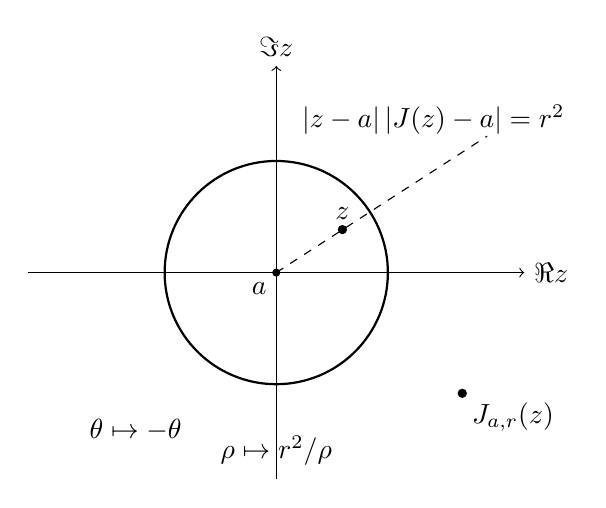
\begin{tikzpicture}[scale=1.05]
  \draw[->] (-3,0)--(3,0) node[right] {$\Re z$};
  \draw[->] (0,-2.5)--(0,2.5) node[above] {$\Im z$};
  \draw[thick] (0,0) circle (1.35);
  \fill (0,0) circle (1.4pt) node[below left] {$a$};
  \draw[dashed] (0,0)--(2.55,1.65);
  \fill (0.8,0.52) circle (1.6pt) node[above] {$z$};
  \fill (2.25,-1.46) circle (1.6pt) node[below right] {$J_{a,r}(z)$};
  \node at (1.9,1.85) {$|z-a|\,|J(z)-a|=r^2$};
  \node at (-1.7,-1.9) {$\theta\mapsto-\theta$};
  \node at (0,-2.15) {$\rho\mapsto r^2/\rho$};
\end{tikzpicture}
\caption{The Möbius inversion $J_{a,r}(z)=a+r^2/(z-a)$ sends $\rho e^{i\theta}$ relative to $a$ to $(r^2/\rho)e^{-i\theta}$. The reference circle $|z-a|=r$ is invariant as a set.}
\label{fig:cp-iv-0014-holomorphic-inversion}
\end{figure}


\begin{solution}
Write
\[
z-a=\rho e^{i\theta},
\qquad \rho>0.
\]
For
\[
J_{a,r}(z)=a+\frac{r^2}{z-a}
\]
we obtain
\[
J_{a,r}(z)-a
=
\frac{r^2}{\rho e^{i\theta}}
=
\frac{r^2}{\rho}e^{-i\theta}.
\]
Therefore
\[
|J_{a,r}(z)-a|
=
\frac{r^2}{|z-a|}
\]
and
\[
\operatorname{Arg}(J_{a,r}(z)-a)
\equiv
-\operatorname{Arg}(z-a)
\pmod{2\pi}.
\]
Thus the radius is inverted and the angular coordinate is reflected.

Moreover,
\[
J'_{a,r}(z)=-\frac{r^2}{(z-a)^2}\neq0
\]
for \(z\neq a\), so \(J_{a,r}\) is conformal there. It is a M\"obius transformation of the Riemann sphere, interchanging \(a\) and \(\infty\). If \(|z-a|=r\), then \(|J_{a,r}(z)-a|=r\), so the circle is preserved as a set.
\end{solution}


\begin{problem}[CP-IV-0015]
\label{prob:cp-iv-0015}
(exact restatement of the two tasks)

\noindent\textbf{(a)} Show that the principal value is well defined for all $\zeta_{0}\in\Gamma^{\ast}$, namely that the limit
	\[
	\operatorname{P.V.}\,\frac{1}{2\pi i}\int_{\Gamma}\frac{f(\zeta)}{\zeta-\zeta_{0}}\,d\zeta
	\;:=\;\lim_{\varepsilon\downarrow 0}\,\frac{1}{2\pi i}\int_{\Gamma_{\varepsilon}}
	\frac{f(\zeta)}{\zeta-\zeta_{0}}\,d\zeta
	\]
	exists, where $\Gamma$ is a simple smooth positively oriented curve, $f$ is continuously differentiable on $\Gamma^{\ast}$, and $\Gamma_{\varepsilon}$ is the part of $\Gamma$ that is at least $\varepsilon$–away from $\zeta_{0}$.

	\medskip

	\noindent\textbf{(b)} Show that
	\[
	\operatorname{P.V.}\,\frac{1}{2\pi i}\int_{\Gamma}\frac{f(\zeta)}{\zeta-\zeta_{0}}\,d\zeta
	\;=\;
	\frac{1}{2\pi i}\int_{\Gamma}\frac{f(\zeta)-f(\zeta_{0})}{\zeta-\zeta_{0}}\,d\zeta
	\;+\;\frac{1}{2}\,f(\zeta_{0}).
	\]

	\bigskip\hrule\bigskip

	Let $\Gamma$ be a simple $C^{1}$ positively oriented closed curve in the plane and let $f\in C^{1}(\Gamma)$.
	For $z\in\mathbb{C}\setminus\Gamma$ define the Cauchy transform
	\[
	F(z):=\frac{1}{2\pi i}\int_{\Gamma}\frac{f(\zeta)}{\zeta-z}\,d\zeta.
	\]
	Then $F$ is holomorphic on each component of $\mathbb{C}\setminus\Gamma$.
	As $z\to\zeta_{0}\in\Gamma$, the kernel $(\zeta-z)^{-1}$ has a simple pole on the contour; the principal value removes a small arc around $\zeta_{0}$ and takes the limit as its length shrinks to $0$.

	\bigskip\hrule\bigskip
\end{problem}

% Designed Companion Part IV figure
% Intended for \input{...} beside the matching canonical problem.
\begin{figure}[ht]
\centering
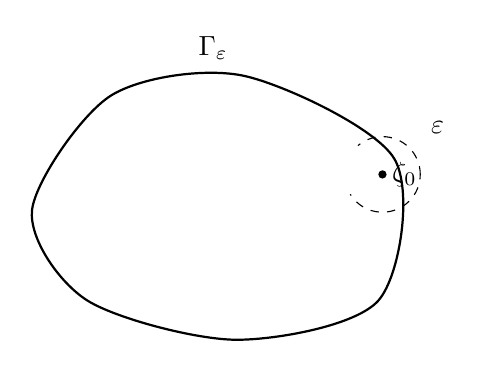
\begin{tikzpicture}[scale=1.0]
  \draw[thick] plot[smooth cycle] coordinates {(-2.4,0) (-1.4,1.45) (0.3,1.7) (2.2,0.65) (2,-1.15) (0.2,-1.65) (-1.7,-1.15)};
  \fill (2.05,0.45) circle (1.5pt) node[right] {$\zeta_0$};
  \draw[dashed] (2.05,0.45) circle (0.48);
  \draw[white,line width=5pt] (1.72,0.83) arc[start angle=135,end angle=215,radius=0.48];
  \node at (2.75,1.05) {$\varepsilon$};
  \node at (-0.1,2.05) {$\Gamma_\varepsilon$};
\end{tikzpicture}
\caption{The principal value contour $\Gamma_\varepsilon$ is obtained by deleting the small arc of $\Gamma$ inside the $\varepsilon$-disk about the singular boundary point $\zeta_0$ and then letting $\varepsilon\downarrow0$.}
\label{fig:cp-iv-0015-principal-value-deleted-arc}
\end{figure}


\begin{solution}
\subsection*{Solution to (a): existence of the principal value}

	Fix $\zeta_{0}\in\Gamma$.
	Split the integrand into a regular part and a pure singular kernel:
	\[
	\frac{f(\zeta)}{\zeta-\zeta_{0}}
	\;=\;
	\underbrace{\frac{f(\zeta)-f(\zeta_{0})}{\zeta-\zeta_{0}}}_{\text{regular near }\zeta_{0}}
	\;+\;
	\underbrace{\frac{f(\zeta_{0})}{\zeta-\zeta_{0}}}_{\text{pure kernel}}.
	\tag{1}
	\]

	\emph{Regular part.}
	Since $f\in C^{1}(\Gamma)$, there is a constant $C$ with
	\[
	|f(\zeta)-f(\zeta_{0})|\le C\,|\zeta-\zeta_{0}|
	\quad\text{for }\zeta\text{ near }\zeta_{0}.
	\]
	Hence the quotient $\dfrac{f(\zeta)-f(\zeta_{0})}{\zeta-\zeta_{0}}$ is bounded and continuous on $\Gamma$ (interpreted by continuity at $\zeta_{0}$).
	Therefore
	\[
	\int_{\Gamma_{\varepsilon}}\frac{f(\zeta)-f(\zeta_{0})}{\zeta-\zeta_{0}}\,d\zeta
	\quad\text{converges as }\varepsilon\downarrow 0,
	\]
	so its contribution to the principal value has a proper limit (indeed, it is just the ordinary integral over $\Gamma$).

	\medskip

	\emph{Pure kernel.}
	On the small missing arc of radius $\varepsilon$ around $\zeta_{0}$ the integral
	\[
	\int\frac{d\zeta}{\zeta-\zeta_{0}}
	\]
	is $\pm\,\pi i$ in the limit (half of the $2\pi i$ residue), with the sign determined by whether the indentation is taken inside or outside, together with the positive orientation of $\Gamma$.
	Thus the contribution of the pure kernel to the truncated integral is uniformly bounded and tends, in the principal value sense, to the finite number $\dfrac{1}{2}\,2\pi i\cdot \dfrac{f(\zeta_{0})}{2\pi i}=\dfrac{1}{2}f(\zeta_{0})$ (precisely accounted for in part (b) below).

	\medskip

	Combining the two parts from (1) shows that the limit defining
	\[
	\operatorname{P.V.}\,\frac{1}{2\pi i}\int_{\Gamma}\frac{f(\zeta)}{\zeta-\zeta_{0}}\,d\zeta
	\]
	exists for every $\zeta_{0}\in\Gamma$.

	\bigskip\hrule\bigskip

	\subsection*{Solution to (b): decomposition formula with the $\tfrac12 f(\zeta_{0})$ term}

	Start from the splitting \textnormal{(1)} and integrate over $\Gamma_{\varepsilon}$:
	\[
	\frac{1}{2\pi i}\int_{\Gamma_{\varepsilon}}\frac{f(\zeta)}{\zeta-\zeta_{0}}\,d\zeta
	=
	\frac{1}{2\pi i}\int_{\Gamma_{\varepsilon}}\frac{f(\zeta)-f(\zeta_{0})}{\zeta-\zeta_{0}}\,d\zeta
	+\frac{f(\zeta_{0})}{2\pi i}\int_{\Gamma_{\varepsilon}}\frac{d\zeta}{\zeta-\zeta_{0}}.
	\]
	Let $\varepsilon\downarrow 0$.
	The first term converges to the \emph{ordinary} integral over $\Gamma$ because its integrand is bounded and continuous on $\Gamma$:
	\[
	\lim_{\varepsilon\downarrow 0}\frac{1}{2\pi i}\int_{\Gamma_{\varepsilon}}\frac{f(\zeta)-f(\zeta_{0})}{\zeta-\zeta_{0}}\,d\zeta
	=
	\frac{1}{2\pi i}\int_{\Gamma}\frac{f(\zeta)-f(\zeta_{0})}{\zeta-\zeta_{0}}\,d\zeta.
	\]
	For the second term,
	\[
	\lim_{\varepsilon\downarrow 0}\frac{1}{2\pi i}\int_{\Gamma_{\varepsilon}}\frac{d\zeta}{\zeta-\zeta_{0}}
	=\frac{1}{2},
	\]
	because the missing small arc carries half of the $2\pi i$ residue at $\zeta=\zeta_{0}$ (with the positive orientation prescribed in the statement).
	Therefore,
	\[
	\operatorname{P.V.}\,\frac{1}{2\pi i}\int_{\Gamma}\frac{f(\zeta)}{\zeta-\zeta_{0}}\,d\zeta
	=
	\frac{1}{2\pi i}\int_{\Gamma}\frac{f(\zeta)-f(\zeta_{0})}{\zeta-\zeta_{0}}\,d\zeta
	+\frac{1}{2}\,f(\zeta_{0}),
	\]
	as required.

	\bigskip\hrule\bigskip
\end{solution}

\begin{problem}[CP-IV-0017]
\label{prob:cp-iv-0017}
\par\noindent\textbullet\quad (\textbf{Quick diagnostics})
	For each matrix, compute $(A,B)$ and decide if $T$ is complex-linear.
	\[
	\text{(a) }\begin{psmallmatrix}2&1\\ -1&2\end{psmallmatrix}\quad
	\text{(b) }\begin{psmallmatrix}1&1\\ 1&1\end{psmallmatrix}\quad
	\text{(c) }\begin{psmallmatrix}0&1\\ 1&0\end{psmallmatrix}.
	\]
	\emph{Solution.}
	(a) $A=2+i(-1-1)/2=2-i,\ B=\tfrac{2-2}{2}+i\tfrac{-1+1}{2}=0$ $\Rightarrow$ holomorphic.
	(b) $A=1+i\,0=1,\ B=0+i\,1=i$ $\Rightarrow$ not holomorphic.
	(c) $A=\tfrac{0+0}{2}+i\,\tfrac{1-1}{2}=0,\ B=\tfrac{0-0}{2}+i\,\tfrac{1+1}{2}=i$ $\Rightarrow$ not holomorphic.
\end{problem}

\begin{solution}
For a real-linear map
\[
T(x+iy)=(ax+by)+i(cx+dy)
\]
one has the decomposition
\[
T(z)=Az+B\overline z,
\]
where
\[
A=\frac{a+d}{2}+i\,\frac{c-b}{2},
\qquad
B=\frac{a-d}{2}+i\,\frac{c+b}{2}.
\]
The map is complex-linear, hence holomorphic, exactly when \(B=0\).

For
\[
\begin{pmatrix}2&1\\-1&2\end{pmatrix}
\]
we get
\[
A=2-i,\qquad B=0,
\]
so the map is holomorphic.

For
\[
\begin{pmatrix}1&1\\1&1\end{pmatrix}
\]
we get
\[
A=1,\qquad B=i,
\]
so it is not holomorphic.

For
\[
\begin{pmatrix}0&1\\1&0\end{pmatrix}
\]
we get
\[
A=0,\qquad B=i,
\]
so
\[
T(z)=i\overline z.
\]
This is antiholomorphic, not holomorphic.
\end{solution}


\begin{problem}[CP-IV-0031]
\label{prob:cp-iv-0031}
\par\noindent\textbullet\quad Use Cauchy’s integral formula to compute
	\[
	\int_{|z|=1}\frac{e^{\alpha z}}{2z^{2}-5z+2}\,dz,\qquad \alpha\in\mathbb C.
	\]

	\par\noindent\textbullet\quad By considering the real part of a suitable complex integral, show that for $r\in(0,1)$,
	\[
	\int_{0}^{\pi}\frac{\cos(n\theta)}{1-2r\cos\theta+r^{2}}\,d\theta=\frac{\pi r^{n}}{1-r^{2}},
	\qquad
	\int_{0}^{2\pi}\cos(\cos\theta)\cosh(\sin\theta)\,d\theta=2\pi .
	\]

Cauchy’s integral formula: if $f$ is holomorphic on and inside a simple closed curve $\gamma$, then
$\displaystyle \int_\gamma \frac{f(z)}{z-a}\,dz=2\pi i\,f(a)$ for $a$ inside $\gamma$.
Also, with $z=e^{i\theta}$ one has $d\theta=\frac{dz}{iz}$ and
$1-2r\cos\theta+r^{2}=(1-rz)(1-rz^{-1})=\frac{(z-r)(1-rz)}{z}$.
\end{problem}

% Designed Companion Part IV figure
% Intended for \input{...} beside the matching canonical problem.
\begin{figure}[ht]
\centering
\begin{tikzpicture}[scale=1.15]
  \draw[->] (-2.6,0)--(3.0,0) node[right] {$\Re z$};
  \draw[->] (0,-2.2)--(0,2.2) node[above] {$\Im z$};
  \draw[thick] (0,0) circle (1.35);
  \fill (0.5,0) circle (1.7pt) node[above] {$1/2$};
  \fill (2,0) circle (1.7pt) node[above] {$2$};
  \node at (-0.7,1.65) {$|z|=1$};
  \node at (0,-2.65) {$2z^2-5z+2=2(z-\tfrac12)(z-2)$};
\end{tikzpicture}
\caption{For the first contour integral, the denominator has poles at $z=1/2$ and $z=2$. Only $z=1/2$ lies inside the positively oriented unit circle.}
\label{fig:cp-iv-0031-unit-circle-rational-poles}
\end{figure}


\begin{solution}
\emph{(i)} Factor $2z^{2}-5z+2=2(z-2)\bigl(z-\tfrac12\bigr)$. On $|z|=1$ only $z=\tfrac12$ lies inside.
Hence
\[
\int_{|z|=1}\frac{e^{\alpha z}}{2z^{2}-5z+2}\,dz
=2\pi i\cdot \operatorname{Res}\!\left(\frac{e^{\alpha z}}{2(z-2)\bigl(z-\tfrac12\bigr)};\ \tfrac12\right)
=2\pi i\cdot \frac{e^{\alpha/2}}{2(\tfrac12-2)}
=-\,\frac{2\pi i}{3}\,e^{\alpha/2}.
\]

\medskip
\emph{(ii-a)} Let
\[
I_n=\int_{0}^{2\pi}\frac{e^{in\theta}}{1-2r\cos\theta+r^{2}}\,d\theta.
\]
With $z=e^{i\theta}$ and $d\theta=\frac{dz}{iz}$,
\[
I_n=\oint_{|z|=1}\frac{z^{n}}{(z-r)(1-rz)}\,\frac{dz}{i}.
\]
Only $z=r$ lies inside, giving $\operatorname{Res}=\dfrac{r^{n}}{1-r^{2}}$. Thus
\[
I_n=2\pi\,\frac{r^{n}}{1-r^{2}},\qquad
\int_{0}^{2\pi}\frac{\cos(n\theta)}{1-2r\cos\theta+r^{2}}\,d\theta
=\Re I_n=\frac{2\pi r^{n}}{1-r^{2}}.
\]
Halving the interval,
\[
\int_{0}^{\pi}\frac{\cos(n\theta)}{1-2r\cos\theta+r^{2}}\,d\theta
=\frac{\pi r^{n}}{1-r^{2}}.
\]

\medskip
\emph{(ii-b)} Using
$\cos(\cos\theta)\cosh(\sin\theta)=\tfrac12\big(e^{i e^{i\theta}}+e^{-i e^{i\theta}}\big)$,
\[
\int_{0}^{2\pi}\cos(\cos\theta)\cosh(\sin\theta)\,d\theta
=\frac12\oint_{|z|=1}\frac{e^{iz}+e^{-iz}}{iz}\,dz
=\frac{1}{2i}\cdot 2\pi i\,\bigl(e^{0}+e^{0}\bigr)=2\pi.
\]
\end{solution}

\begin{problem}[CP-IV-0034]
\label{prob:cp-iv-0034}
an image sheaf larger than the objectwise image

Let

	\[
	X=\mathbb C^\times
	=
	\mathbb C\setminus\{0\}.
	\]

	Let $\mathcal O_X$ be the sheaf of holomorphic functions on $X$, and let
	$\mathcal O_X^\times$ be the sheaf of nowhere-zero holomorphic functions.

	There is a morphism of sheaves

	\[
	\exp:\mathcal O_X\to \mathcal O_X^\times
	\]

	given by

	\[
	f\longmapsto e^{2\pi i f}.
	\]

	Locally, every nowhere-zero holomorphic function has a holomorphic logarithm.
	Therefore, locally, every section of $\mathcal O_X^\times$ lies in the image of
	$\exp$.

	Hence the sheaf image is

	\[
	\im(\exp)=\mathcal O_X^\times.
	\]

	However, globally, the function

	\[
	g(z)=z
	\]

	on $\mathbb C^\times$ has no global holomorphic logarithm.

	Indeed, if there were a holomorphic function

	\[
	h:\mathbb C^\times\to\mathbb C
	\]

	such that

	\[
	e^{2\pi i h(z)}=z,
	\]

	then $h$ would define a global branch of the logarithm on $\mathbb C^\times$.
	But such a branch does not exist.

	Therefore

	\[
	z\notin
	\im\left(
	\mathcal O_X(X)\to \mathcal O_X^\times(X)
	\right).
	\]

	Thus

	\[
	\boxed{
		\im_{\text{sheaf}}(\exp)=\mathcal O_X^\times,
	}\]

	but

	\[
	\boxed{
		\im\left(
		\mathcal O_X(X)\to \mathcal O_X^\times(X)
		\right)
		\neq
		\mathcal O_X^\times(X).
	}\]

	This is one of the most important examples of the difference between global
	image and sheaf image.

	\[
	\boxed{
		\text{Sheaf image means locally image, not globally image.}
	}\]
\end{problem}

\begin{solution}
Let \(X=\mathbb C^\times\), and consider the exponential morphism
\[
\exp:\mathcal O_X\longrightarrow\mathcal O_X^\times.
\]
Every nowhere-zero holomorphic function has a local holomorphic logarithm, so every germ in \(\mathcal O_X^\times\) lies locally in the image of \(\exp\). Hence the sheaf image is all of \(\mathcal O_X^\times\).

However, the objectwise image on global sections can be smaller. Consider the global unit
\[
g(z)=z\in\mathcal O_X^\times(X).
\]
If \(g=e^F\) for some global \(F\in\mathcal O_X(X)\), then differentiation would give
\[
F'(z)=\frac1z.
\]
Integrating around the unit circle,
\[
0=\oint_{|z|=1}F'(z)\,dz
=
\oint_{|z|=1}\frac{dz}{z}
=
2\pi i,
\]
a contradiction. Thus \(z\) has local holomorphic logarithms but no global one.

Therefore
\[
\operatorname{im}_{\mathrm{sheaf}}(\exp)=\mathcal O_X^\times,
\]
while
\[
\exp\bigl(\mathcal O_X(X)\bigr)
\subsetneq
\mathcal O_X^\times(X).
\]
This gives the desired distinction between sheaf image and objectwise image.
\end{solution}


\begin{problem}[CP-IV-0035]
\label{prob:cp-iv-0035}
a line mapped to the real axis

Now let $L$ be a straight line instead of a circle. Take, for instance,
	the imaginary axis
	\[
	L = \{ z = i y : y\in\mathbb R\},
	\]
	and choose three distinct points on $L$:
	\[
	a = i,\qquad b=-i,\qquad c=0.
	\]
	The corresponding cross-ratio map
	\[
	\Phi(z)
	= \frac{(z-a)(c-b)}{(z-b)(c-a)}
	\]
	again satisfies
	\[
	\Phi(a)=0,\qquad \Phi(b)=\infty,\qquad \Phi(c)=1,
	\]
	and sends the whole line $L$ onto the real axis
	$\mathbb R\cup\{\infty\}$. As before, the two sides of $L$ are mapped
	onto the upper and lower half-planes:
	\[
	\text{one side of } L \;\longmapsto\; \{ w : \Im w > 0\},\qquad
	\text{the other side} \;\longmapsto\; \{ w : \Im w < 0\}.
	\]

	Figure~\ref{fig:crossratio-line-z-plane} shows the line $L$ and some
	sample points on each side, distinguished by the sign of $\Im \Phi(z)$.
	Figure~\ref{fig:crossratio-line-w-plane} illustrates their images under
	$\Phi$: the line becomes the real axis, with $\Phi(a)=0$ and
	$\Phi(c)=1$, and the two sides become the upper and lower half-planes.
\begin{figure}[ht]
  \centering
  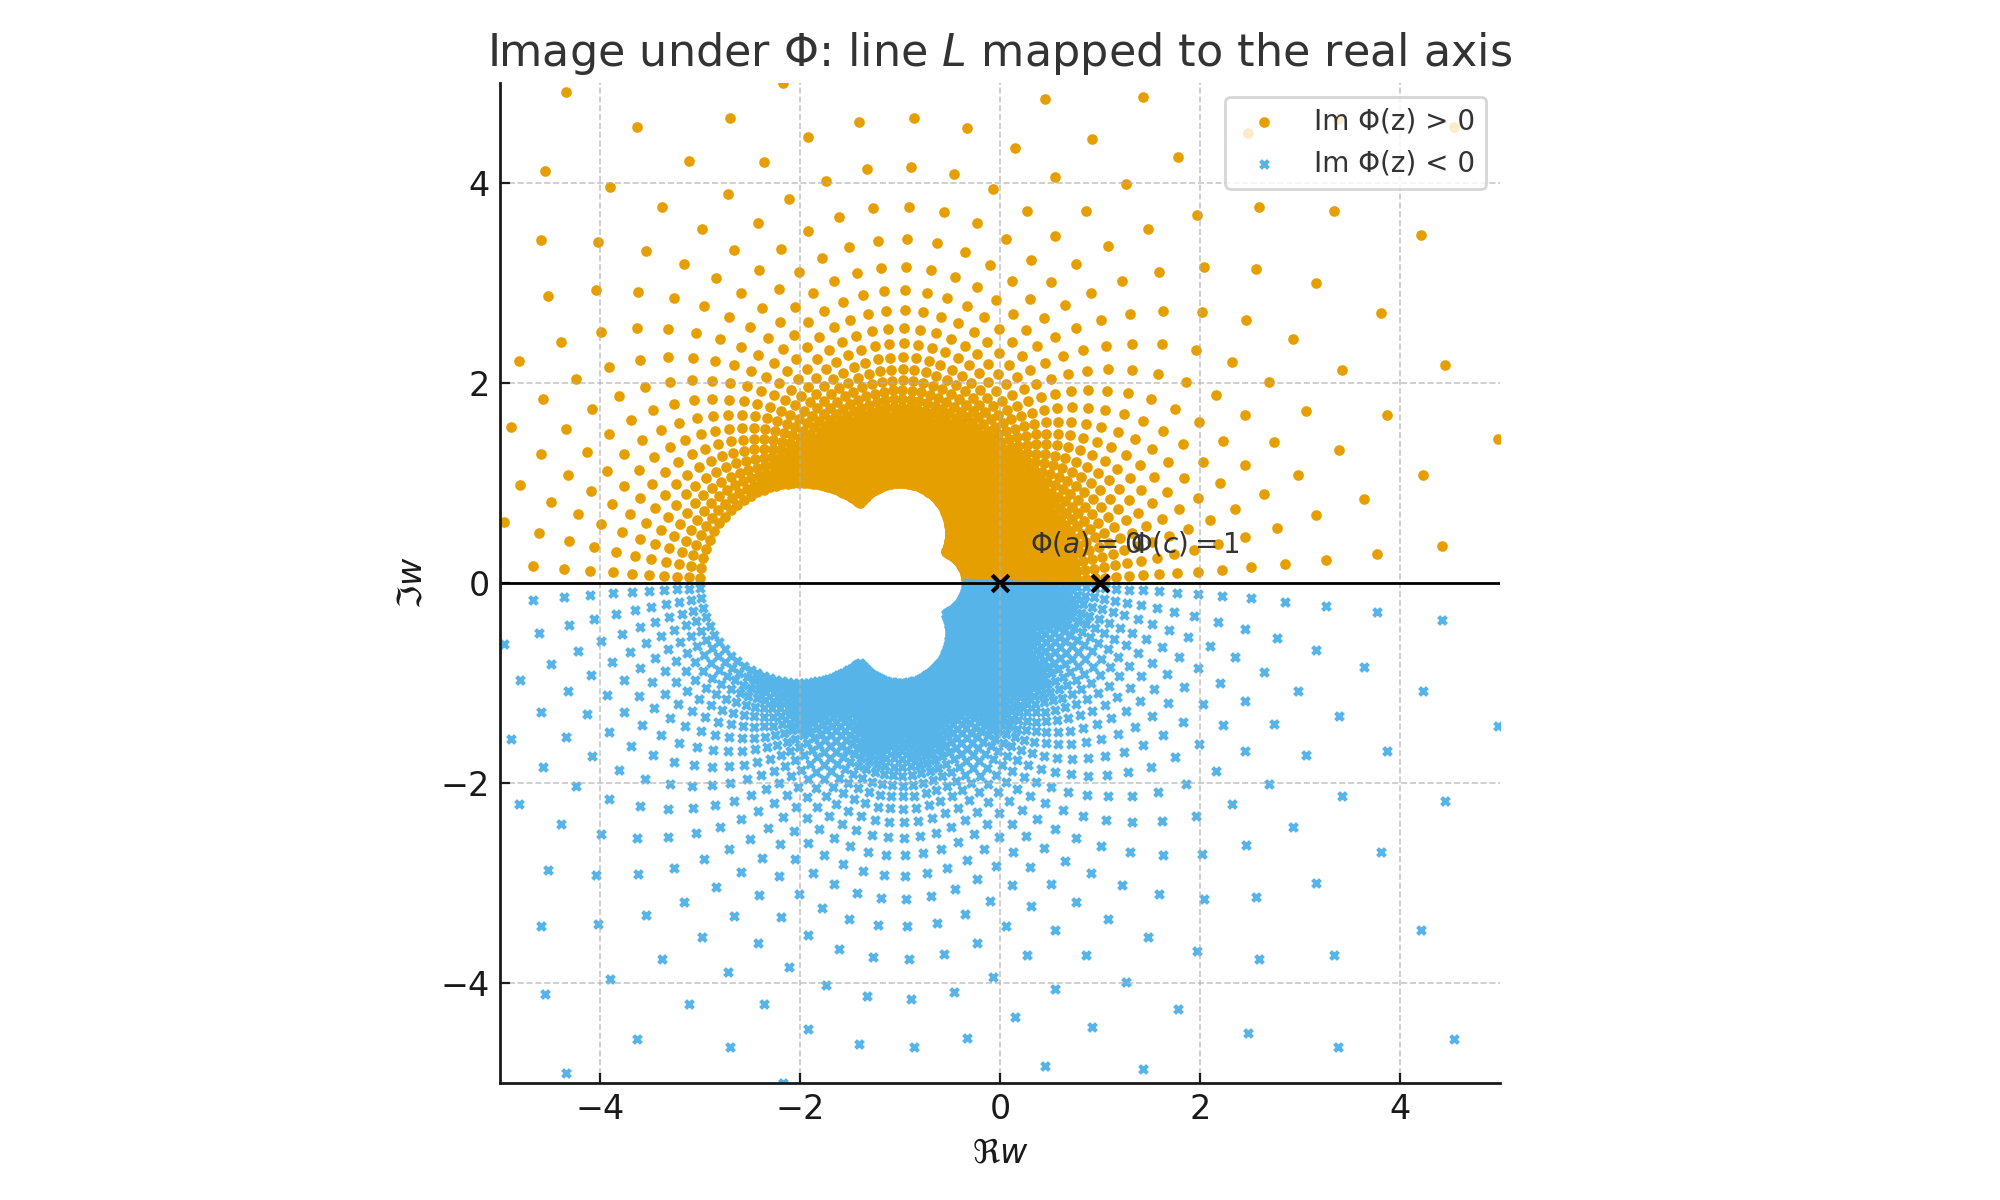
\includegraphics[width=0.78\textwidth]{figures/part04/cp_iv_0035_crossratio_line_w_plane.png}
  \caption{Source-backed Part IV figure: crossratio line w plane.}
  \label{fig:crossratio-line-w-plane}
\end{figure}

\begin{figure}[ht]
  \centering
  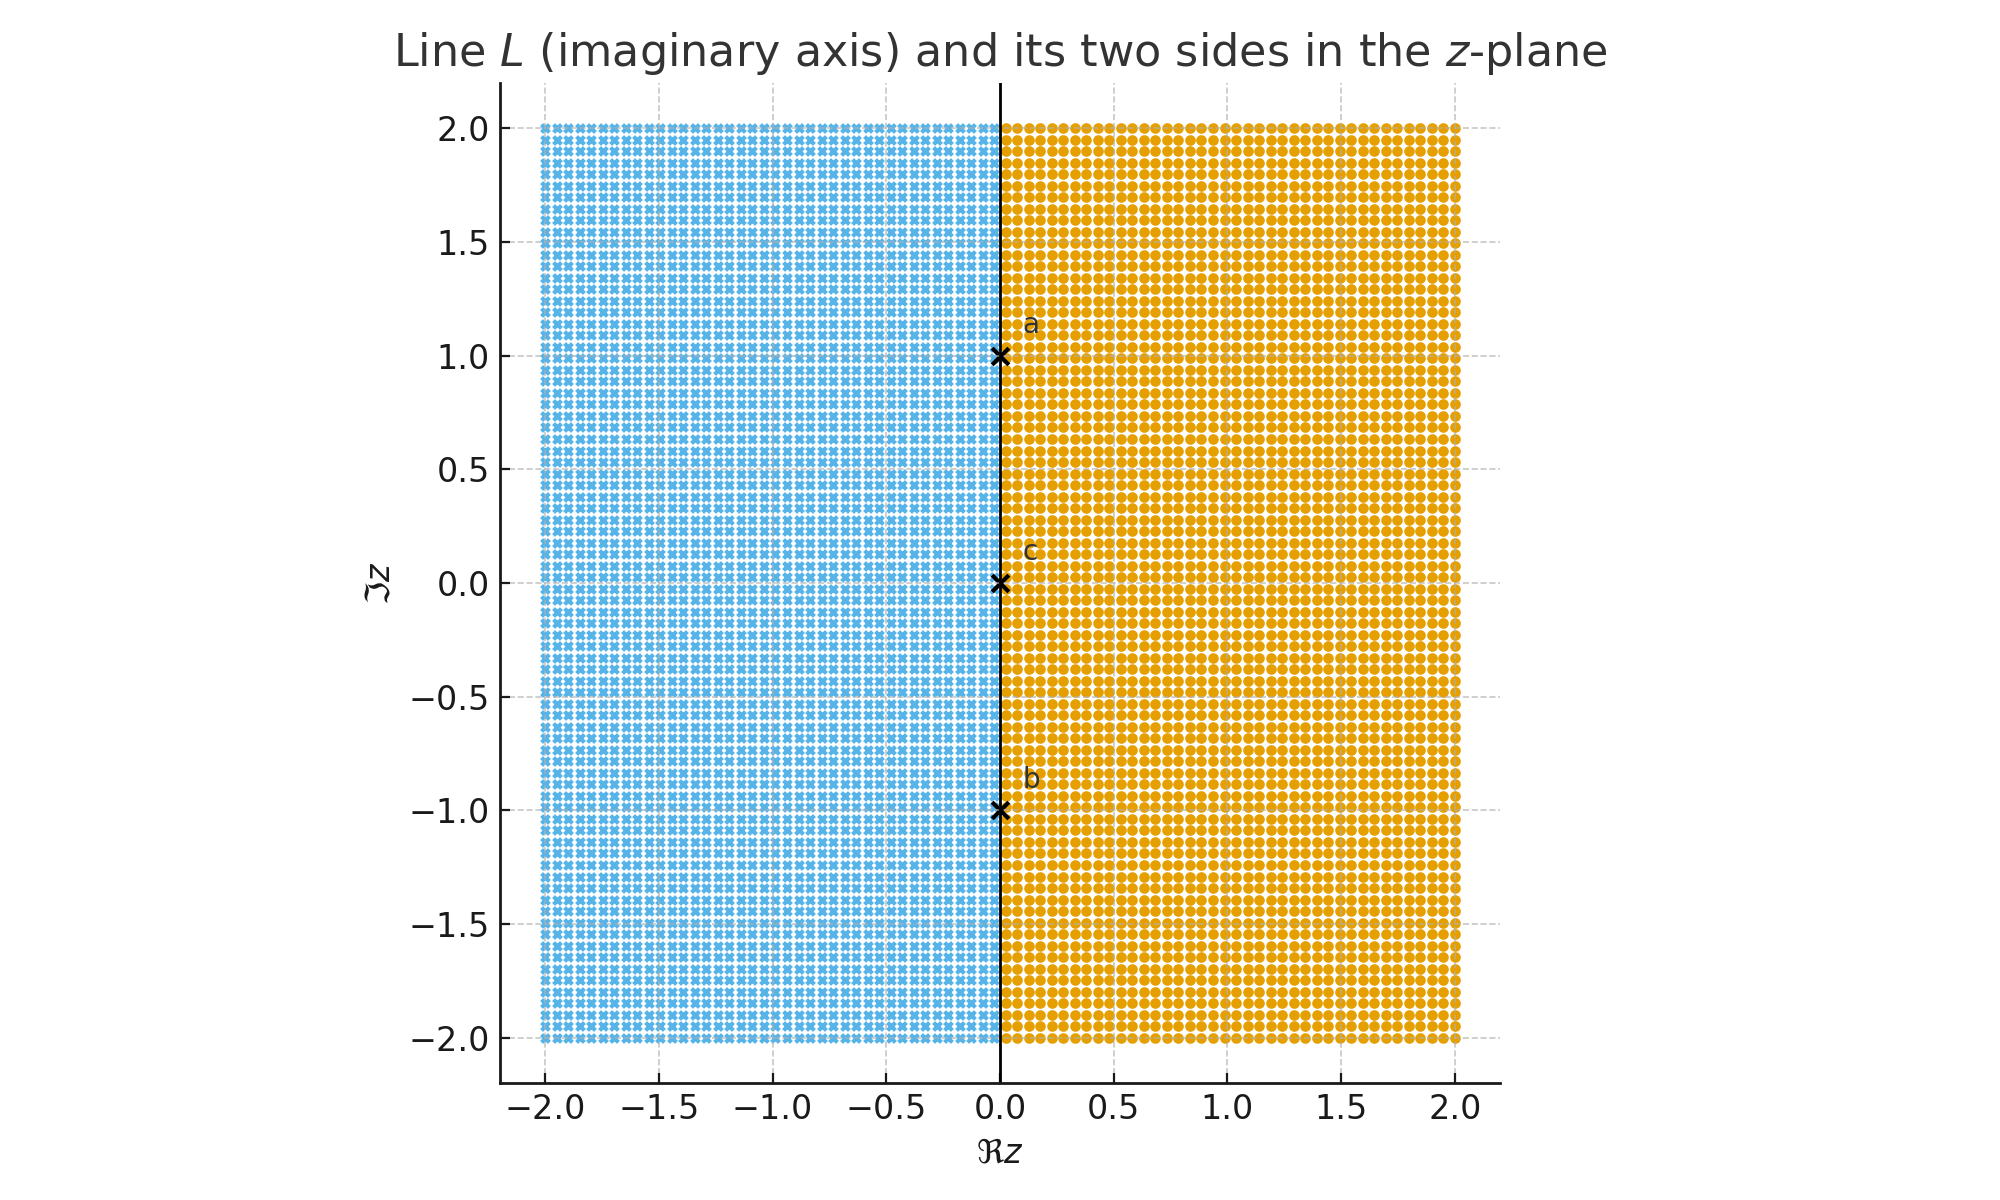
\includegraphics[width=0.78\textwidth]{figures/part04/cp_iv_0035_crossratio_line_z_plane.png}
  \caption{Source-backed Part IV figure: crossratio line z plane.}
  \label{fig:crossratio-line-z-plane}
\end{figure}


	\medskip

	\clearpage

Let $H_1,H_2$ be half-planes with boundary arcs $L_1,L_2$.
Choose boundary triples
\[
a,b,c \in L_1, \qquad A,B,C \in L_2
\]
in the same cyclic order as seen from the chosen sides of $H_1,H_2$.

First send $L_1$ to the real axis by the cross-ratio map
\[
\Phi(z) := \frac{(z-a)(c-b)}{(z-b)(c-a)}.
\]
Then $\Phi(a)=0$, $\Phi(b)=\infty$, $\Phi(c)=1$, and the two sides of
$L_1$ correspond to the half-planes $\Im\Phi(z)\gtrless 0$.

Next send $L_2$ to the real axis by
\[
\Psi(w) := \frac{(w-A)(C-B)}{(w-B)(C-A)},
\]
so that $\Psi(A)=0$, $\Psi(B)=\infty$, $\Psi(C)=1$.

The desired map $T : H_1 \to H_2$ is given by
\[
\Psi\bigl(T(z)\bigr) = \Phi(z),
\qquad\text{i.e.}\qquad
T(z) = \Psi^{-1}(\Phi(z)).
\]
Solving for $\Psi^{-1}$ yields the explicit formula
\[
T(z)
= \frac{A(C-B) - \Phi(z)\, B(C-A)}{(C-B) - \Phi(z)\,(C-A)},
\qquad
\Phi(z) = \frac{(z-a)(c-b)}{(z-b)(c-a)}.
\]
Then
\[
T(a)=A,\qquad T(b)=B,\qquad T(c)=C,
\]
and $T$ maps the chosen side of $H_1$ biholomorphically onto the chosen
side of $H_2$. If the orientation of the half-plane is reversed, one may
replace $\Phi$ by $-\Phi$ or interchange two of the boundary points to
flip the side.
\end{problem}

\begin{solution}
For
\[
a=i,\qquad b=-i,\qquad c=0,
\]
the cross-ratio map is
\[
\Phi(z)
=
\frac{(z-i)(0+i)}{(z+i)(0-i)}
=
-\frac{z-i}{z+i}.
\]
If \(z=iy\) lies on the imaginary axis, then
\[
\Phi(iy)
=
-\frac{y-1}{y+1}\in\mathbb R\cup\{\infty\}.
\]
Hence the boundary line is mapped to the extended real axis, with
\[
\Phi(i)=0,\qquad
\Phi(-i)=\infty,\qquad
\Phi(0)=1.
\]
Because a M\"obius transformation maps generalized circles to generalized circles and is conformal away from its pole, the two components of the complement of the imaginary axis are mapped to the two half-planes bounded by \(\mathbb R\). Checking one test point determines which side goes to \(\Im w>0\).

For general half-planes \(H_1,H_2\), choose boundary triples \(a,b,c\in\partial H_1\) and \(A,B,C\in\partial H_2\) in the same cyclic order and set
\[
\Phi(z)=\frac{(z-a)(c-b)}{(z-b)(c-a)},
\qquad
\Psi(w)=\frac{(w-A)(C-B)}{(w-B)(C-A)}.
\]
Then both maps send their boundary triples to \(0,\infty,1\). Consequently
\[
T=\Psi^{-1}\circ\Phi
\]
satisfies
\[
T(a)=A,\qquad T(b)=B,\qquad T(c)=C.
\]
Solving for \(\Psi^{-1}\) gives
\[
T(z)
=
\frac{A(C-B)-\Phi(z)B(C-A)}
{(C-B)-\Phi(z)(C-A)}.
\]
The cyclic-order hypothesis selects the desired side, so \(T\) maps \(H_1\) biholomorphically onto \(H_2\).
\end{solution}


\begin{problem}[CP-IV-0037]
\label{prob:cp-iv-0037}
Let $U\subset\mathbb C$ be a domain and let $(f_n)$ be a sequence of univalent
(holomorphic injective) functions $f_n:U\to\mathbb C$ such that
$f_n\to f$ uniformly on every compact $K\Subset U$.
Show that the limit $f$ is either univalent or constant.

\bigskip

  We collect the tools we use and the exact way they are applied.

\medskip

\textbf{Rouch\'e's Theorem.}
Let $g,h$ be holomorphic on and inside a simple closed curve $\gamma$.
If $|h(z)|<|g(z)|$ for all $z\in\gamma$, then $g$ and $g+h$ have the same number
of zeros (counted with multiplicity) in the interior of $\gamma$.

\emph{Application here.}
Fix $w\in\mathbb C$. If $f(z_0)=w$ and $z_0$ is the only zero of $f-w$ in a small disc $D$
(with $|f(z)-w|>0$ on $\partial D$), then the uniform convergence on $\partial D$ gives
$|f_n-f|<|f-w|$ there for all large $n$.
Hence $f_n-w$ and $f-w$ have the same zero count in $D$; in particular, $f_n(z)=w$
has at least one solution in $D$ for all large $n$.

\medskip

\textbf{Hurwitz's Theorem.}
If $g_n\to g$ uniformly on compacta in a domain and each $g_n$ is holomorphic
and \emph{non-vanishing}, then either $g\equiv 0$ or $g$ is non-vanishing.
Equivalently, zeros of $g$ are locally the limits of zeros of $g_n$, counted with multiplicity.

\emph{Application here (derivative version).}
For univalent $f_n$, the inverse function theorem ensures $f_n'(z)\neq 0$ on $U$.
If $f$ were non-constant \emph{and} had a critical point $f'(z_0)=0$, then by Hurwitz
applied to $g_n=f_n'$ we would get a contradiction, since $g_n$ never vanish.
Thus a non-constant limit $f$ must satisfy $f'(z)\neq 0$ everywhere (hence be locally injective).

\medskip

\textbf{Two consequences for univalent maps.}
(i) If $f$ is holomorphic and injective on $U$, then $f'(z)\neq 0$ for all $z\in U$.
(ii) If $f(z_1)=f(z_2)=w$ with $z_1\neq z_2$, then by Rouch\'e the value $w$ must be
assumed by $f_n$ in disjoint neighborhoods of $z_1$ and $z_2$ for all large $n$,
contradicting injectivity of $f_n$.

\bigskip

Assume $f$ is not constant.
Suppose, towards a contradiction, that $f$ is not injective: pick
$z_1\neq z_2$ in $U$ with $f(z_1)=f(z_2)=:w$.

Choose disjoint closed discs $\overline{D_1},\overline{D_2}\Subset U$ centered at
$z_1,z_2$, respectively, so small that
\[
f(\partial D_j)\cap\{w\}=\varnothing
\quad\text{and}\quad
\text{$f-w$ has no zeros in $\overline{D_j}$ except at $z_j$}
\]
for $j=1,2$.
Uniform convergence on $\partial D_j$ yields $|f_n-f|<|f-w|$ there for all $n\ge N$,
hence, by Rouch\'e, $f_n-w$ and $f-w$ have the same number of zeros in $D_j$.
Therefore, for all $n\ge N$, the equation $f_n(z)=w$ has at least one solution in each $D_j$.
Because $D_1\cap D_2=\varnothing$, this gives \emph{two} distinct solutions,
contradicting injectivity of $f_n$.

Thus a non-constant limit $f$ cannot fail to be injective.
Hence $f$ is either univalent or constant.
\hfill$\square$

\bigskip

Assume $f$ is not constant and $f_n\to f$ locally uniformly.
Since each $f_n$ is univalent, $f_n'(z)\neq 0$ for all $z$.
By Hurwitz applied to $(f_n')$, either $f'\equiv 0$ (which would force $f$ to be constant,
contrary to assumption) or $f'(z)\neq 0$ everywhere.
Thus $f$ is a local biholomorphism on $U$; a standard covering-space/plane-domain argument
then promotes local injectivity to global injectivity on $U$, so $f$ is univalent.

\bigskip

	\par\noindent\textbullet\quad \emph{Univalent limit:} $f_n(z)=z+\tfrac1n$ on any domain $U$.
	Then $f_n\to f(z)=z$ (univalent).
	\par\noindent\textbullet\quad \emph{Constant limit:} $f_n(z)=\tfrac1n\,z$ on any domain $U$.
	Then $f_n\to f\equiv 0$ (constant).
	\par\noindent\textbullet\quad \emph{Disk automorphisms:} On $\mathbb D$, $f_n(z)=\dfrac{z}{1-\frac{z}{n}}$ are univalent
	and $f_n\to f(z)=z$ uniformly on compacta.
\end{problem}

% Designed Companion Part IV figure
% Intended for \input{...} beside the matching canonical problem.
\begin{figure}[ht]
\centering
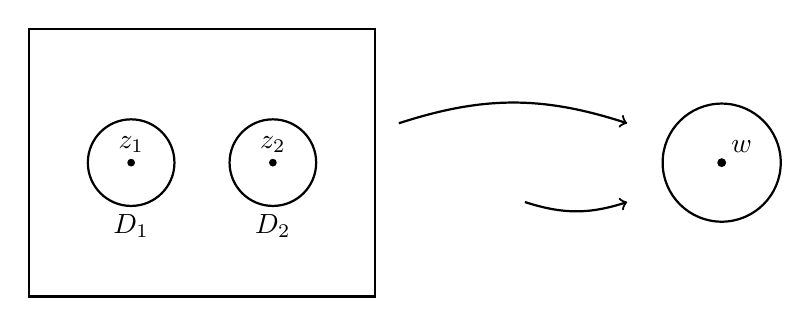
\begin{tikzpicture}[scale=1.0]
  \begin{scope}[xshift=-3.3cm]
    \draw[thick] (-2.2,-1.7) rectangle (2.2,1.7);
    \draw[thick] (-0.9,0) circle (0.55);
    \draw[thick] (0.9,0) circle (0.55);
    \fill (-0.9,0) circle (1.4pt) node[above] {$z_1$};
    \fill (0.9,0) circle (1.4pt) node[above] {$z_2$};
    \node at (-0.9,-0.8) {$D_1$};
    \node at (0.9,-0.8) {$D_2$};
  \end{scope}
  \draw[->,thick] (-0.8,0.5) to[bend left=18] (2.1,0.5);
  \draw[->,thick] (0.8,-0.5) to[bend right=18] (2.1,-0.5);
  \begin{scope}[xshift=3.3cm]
    \draw[thick] (0,0) circle (0.75);
    \fill (0,0) circle (1.6pt) node[above right] {$w$};
  \end{scope}
\end{tikzpicture}
\caption{If a nonconstant limit had $f(z_1)=f(z_2)=w$ with $z_1\ne z_2$, Rouché's theorem on disjoint disks $D_1,D_2$ would force $f_n(z)=w$ to have a solution in each disk for all large $n$, contradicting univalence.}
\label{fig:cp-iv-0037-rouche-two-fibers}
\end{figure}


\begin{solution}
Assume that the locally uniform limit \(f\) is not constant. We show that it is injective.

Suppose instead that
\[
f(z_1)=f(z_2)=w,
\qquad z_1\neq z_2.
\]
Choose disjoint discs \(D_1,D_2\Subset U\) around \(z_1,z_2\) so small that \(f-w\) has no zeros on either boundary and has at least one zero in each disc. Since \(f_n\to f\) uniformly on the compact set
\[
\partial D_1\cup\partial D_2,
\]
for all sufficiently large \(n\),
\[
|f_n-f|<|f-w|
\]
on both boundaries. Rouch\'e's theorem then implies that \(f_n-w\) and \(f-w\) have the same number of zeros in each \(D_j\). Thus \(f_n(z)=w\) has a solution in \(D_1\) and another in \(D_2\), contradicting injectivity of \(f_n\).

Hence a nonconstant limit is injective. Therefore the locally uniform limit of univalent functions is either univalent or constant.

As a consistency check, univalence of each \(f_n\) also gives \(f_n'\neq0\). Since \(f_n'\to f'\) locally uniformly, Hurwitz's theorem implies that either \(f'\equiv0\) or \(f'\) never vanishes. In the nonconstant case \(f'\not\equiv0\), so \(f\) is locally biholomorphic everywhere.
\end{solution}


\begin{problem}[CP-IV-0039]
\label{prob:cp-iv-0039}
(General mixed map).

Take $A=1+\tfrac12 i$, $B=0.6-0.2i$. Then
\[
\det DT=|A|^2-|B|^2=(1^2+\tfrac{1}{4})-(0.6^2+0.2^2)=1.25-0.40=0.85>0,
\]
so $T$ is invertible and orientation-preserving, but not holomorphic ($B\neq0$).
Singular values are $\sigma_{\max}=|A|+|B|\approx \sqrt{1.25}+ \sqrt{0.40}$ and
$\sigma_{\min}=||A|-|B||$, giving principal stretches of the ellipse.

For any $T(z)=Az+B\bar z$, the image of the unit circle is an ellipse whenever $|A|\neq|B|$; it degenerates to a segment/point when $|A|=|B|$.
Holomorphicity is equivalent to $B=0$; antiholomorphicity (composition with conjugation) corresponds to $A=0$.
\end{problem}

\begin{solution}
Here
\[
A=1+\frac{i}{2},
\qquad
B=0.6-0.2i.
\]
For a real-linear map \(T(z)=Az+B\overline z\), the Jacobian determinant is
\[
J_T=|A|^2-|B|^2.
\]
Thus
\[
J_T
=
\left(1+\frac14\right)
-
\left(0.6^2+0.2^2\right)
=
1.25-0.40
=
0.85>0.
\]
Hence \(T\) is invertible and orientation-preserving.

Since \(B\neq0\), the map is not complex-linear and therefore is not holomorphic. The singular values are
\[
\sigma_{\max}=|A|+|B|,
\qquad
\sigma_{\min}=\bigl||A|-|B|\bigr|.
\]
Because \(|A|\neq|B|\), the image of the unit circle is a genuine ellipse whose semiaxis lengths are these two singular values. In general, \(B=0\) is precisely the holomorphic case, \(A=0\) the antiholomorphic case, and \(|A|=|B|\) is the degenerate case.
\end{solution}


\begin{problem}[CP-IV-0044]
\label{prob:cp-iv-0044}
Weierstrass data: immersion criterion

Let $D\subset\mathbb C$, and $f$ and $g$ be functions on $D$ giving a Weierstrass representation of a
	parametrisation $\phi$. Show that $\phi$ is an immersion iff $f$ vanishes only at the poles of $g$ and the
	order of its zero at such a point is \emph{exactly twice} the order of the pole of $g$.

	\medskip
	\textbf{Solution.}
	In Weierstrass form one may write (up to an overall constant depending on convention)
	\[
	\phi_z = \big((1-g^2)f,\; i(1+g^2)f,\; 2gf\big),
	\]
	a holomorphic $\mathbb C^3$-valued 1-form. The map is an immersion iff $\phi_z\neq 0$ everywhere.

	If $g$ is holomorphic at $p$ and $f(p)=0$, then all components of $\phi_z$ vanish at $p$, so $\phi$ is not an
	immersion. Hence $f$ may vanish only at poles of $g$.

	Now let $p$ be a pole of $g$ of order $m$. Choose a local coordinate $z$ with $z(p)=0$ and write
	\[
	g(z)=a z^{-m}+\cdots,\quad a\neq 0;\qquad f(z)=b z^{n}+\cdots,\quad b\neq 0.
	\]
	Then
	\[
	(1-g^2)f \sim (-a^2)b\,z^{n-2m},\qquad (1+g^2)f\sim (a^2)b\,z^{n-2m},\qquad 2gf\sim 2ab\,z^{n-m}.
	\]
	For $\phi_z$ to be holomorphic at $p$ we need $n-2m\ge 0$, i.e. $n\ge 2m$.
	If $n>2m$, then each component vanishes at $z=0$, hence $\phi_z(p)=0$ and $\phi$ fails to be an immersion.
	Thus we must have $n=2m$, and in that case $(1-g^2)f$ has a nonzero constant term, so $\phi_z(p)\neq 0$.
	Therefore $\phi$ is an immersion iff $f$ vanishes only at poles of $g$ and $\ord_p(f)=2\,\ord_p(\text{pole of }g)$.
	

	\textbf{Goal.} Describe all (simply connected) minimal surfaces in $\mathbb{R}^3$ using holomorphic data.

	\medskip
	\textbf{Setup.}
	Let $\Omega\subset\mathbb{C}$ be simply connected with complex coordinate $z=u+iv$.
	A map $X:\Omega\to\mathbb{R}^3$ is called a \emph{conformal parametrization} if the induced metric has the form
	\[
	ds^2 = e^{2\omega}(du^2+dv^2)
	\quad\text{(equivalently } \langle X_u,X_v\rangle=0,\; |X_u|=|X_v|\text{)}.
	\]
	For conformal parametrizations, the minimality condition $H\equiv 0$ becomes equivalent to harmonicity of $X$:
	\[
	H\equiv 0 \quad\Longleftrightarrow\quad X_{uu}+X_{vv}=0
	\quad\Longleftrightarrow\quad X \text{ is harmonic componentwise.}
	\]

	\medskip
	\textbf{Weierstrass data.}
	Choose
	\[
	g:\Omega\to\widehat{\mathbb{C}} \quad\text{(meromorphic)},\qquad
	\eta = h(z)\,dz \quad\text{(holomorphic 1-form)},
	\]
	such that zeros of $\eta$ cancel poles/zeros of $g$ so that the expressions below are holomorphic.

	Define holomorphic 1-forms
	\[
	\phi_1=\frac12\left(\frac{1}{g}-g\right)\eta,\qquad
	\phi_2=\frac{i}{2}\left(\frac{1}{g}+g\right)\eta,\qquad
	\phi_3=\eta.
	\]
	They satisfy the key identity
	\[
	\phi_1^2+\phi_2^2+\phi_3^2=0.
	\]

	\medskip
	\textbf{Representation theorem.}
	Define
	\[
	X(z)=\Re\int^z (\phi_1,\phi_2,\phi_3).
	\]
	Then $X:\Omega\to\mathbb{R}^3$ is a \emph{conformal minimal immersion} (away from points where all $\phi_k$ vanish).
	Conversely, every conformal minimal immersion on a simply connected domain arises this way.

	\medskip
	\textbf{Meaning of $g$ and $\eta$.}

		\par\noindent\textbullet\quad $g$ is the \emph{stereographic projection of the Gauss map}:
		if $N:\Omega\to S^2$ is the unit normal, then $g=\mathrm{stereo}(N)$.
		\par\noindent\textbullet\quad $\eta$ controls the conformal factor (size) of the metric.

	\medskip
	\textbf{Induced metric (useful formula).}
	The first fundamental form becomes
	\[
	ds^2 = \left(|\phi_1|^2+|\phi_2|^2+|\phi_3|^2\right)
	= \frac{(1+|g|^2)^2}{4|g|^2}\,|\eta|^2,
	\]
	so the parametrization is conformal by construction.

	\medskip
	\textbf{Associate family (catenoid $\leftrightarrow$ helicoid).}
	If $(g,\eta)$ gives a minimal surface, then for any $\alpha\in\mathbb{R}$,
	\[
	(g,\ e^{i\alpha}\eta)
	\]
	gives another minimal surface with the \emph{same metric}; this produces the classical associate family.

	\bigskip

	Take
	\[
	g(z)=z,\qquad \eta = dz.
	\]
	Then
	\[
	X(z)=\Re\int \left(\frac12\left(\frac{1}{z}-z\right),\ \frac{i}{2}\left(\frac{1}{z}+z\right),\ 1\right)\,dz,
	\]
	which yields (after integration and taking real parts) the standard Enneper parametrization.

	\bigskip

	Let
	\[
	g(z)=e^{z},\qquad \eta=dz.
	\]
	Then
	\[
	\phi_1=\frac12(e^{-z}-e^{z})dz=-\sinh(z)\,dz,\qquad
	\phi_2=\frac{i}{2}(e^{-z}+e^{z})dz=i\cosh(z)\,dz,\qquad
	\phi_3=dz.
	\]
	Integrating and taking real parts gives
	\[
	X(z)=\Re\bigl(-\cosh z,\ i\sinh z,\ z\bigr).
	\]
	Writing $z=u+iv$,
	\[
	X(u,v)=\bigl(-\cosh u\cos v,\ -\cosh u\sin v,\ u\bigr),
	\]
	which is a catenoid (up to a rigid motion/sign change).

	If instead we replace $\eta$ by $i\,dz$ (i.e.\ $\alpha=\pi/2$ in the associate family),
	we obtain the helicoid (again up to rigid motion). This illustrates that catenoid and helicoid have the same
	intrinsic metric but differ extrinsically.
\end{problem}

% Designed Companion Part IV figure
% Intended for \input{...} beside the matching canonical problem.
\begin{figure}[ht]
\centering
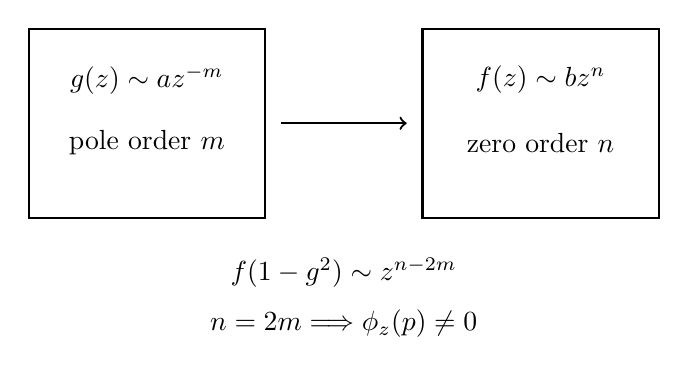
\begin{tikzpicture}[scale=1.0]
  \draw[thick] (-4,1.2) rectangle (-1,-1.2);
  \draw[thick] (1,1.2) rectangle (4,-1.2);
  \node at (-2.5,0.55) {$g(z)\sim a z^{-m}$};
  \node at (-2.5,-0.25) {pole order $m$};
  \node at (2.5,0.55) {$f(z)\sim b z^{n}$};
  \node at (2.5,-0.25) {zero order $n$};
  \draw[->,thick] (-0.8,0)--(0.8,0);
  \node at (0,-1.9) {$f(1-g^2)\sim z^{n-2m}$};
  \node at (0,-2.55) {$n=2m\Longrightarrow\phi_z(p)\ne0$};
\end{tikzpicture}
\caption{Near a pole of $g$ of order $m$ and a zero of $f$ of order $n$, the leading Weierstrass components behave like $z^{n-2m}$. Holomorphicity requires $n\ge2m$, while immersion forces the exact balance $n=2m$.}
\label{fig:cp-iv-0044-weierstrass-order-balance}
\end{figure}


\begin{solution}
In Weierstrass form one may write (up to an overall constant depending on convention)
	\[
	\phi_z = \big((1-g^2)f,\; i(1+g^2)f,\; 2gf\big),
	\]
	a holomorphic $\mathbb C^3$-valued 1-form. The map is an immersion iff $\phi_z\neq 0$ everywhere.

	If $g$ is holomorphic at $p$ and $f(p)=0$, then all components of $\phi_z$ vanish at $p$, so $\phi$ is not an
	immersion. Hence $f$ may vanish only at poles of $g$.

	Now let $p$ be a pole of $g$ of order $m$. Choose a local coordinate $z$ with $z(p)=0$ and write
	\[
	g(z)=a z^{-m}+\cdots,\quad a\neq 0;\qquad f(z)=b z^{n}+\cdots,\quad b\neq 0.
	\]
	Then
	\[
	(1-g^2)f \sim (-a^2)b\,z^{n-2m},\qquad (1+g^2)f\sim (a^2)b\,z^{n-2m},\qquad 2gf\sim 2ab\,z^{n-m}.
	\]
	For $\phi_z$ to be holomorphic at $p$ we need $n-2m\ge 0$, i.e. $n\ge 2m$.
	If $n>2m$, then each component vanishes at $z=0$, hence $\phi_z(p)=0$ and $\phi$ fails to be an immersion.
	Thus we must have $n=2m$, and in that case $(1-g^2)f$ has a nonzero constant term, so $\phi_z(p)\neq 0$.
	Therefore $\phi$ is an immersion iff $f$ vanishes only at poles of $g$ and $\ord_p(f)=2\,\ord_p(\text{pole of }g)$.
\end{solution}

\begin{problem}[CP-IV-0047]
\label{prob:cp-iv-0047}
Complex Geometry

Let \(X\) be a complex manifold, and let
\[
\OO_X
\]
be the sheaf of holomorphic functions on \(X\).

Fix a point
\[
p\in X.
\]

Define
\[
\mathfrak m_p(U)
=
\{f\in \OO_X(U): f(p)=0 \text{ if }p\in U\}.
\]

Then
\[
\mathfrak m_p\subseteq \OO_X.
\]

There is an evaluation morphism
\[
\OO_X\to \CC_p.
\]

The kernel consists of holomorphic functions vanishing at \(p\). Therefore
\[
\ker(\OO_X\to \CC_p)=\mathfrak m_p.
\]

Hence
\[
\OO_X/\mathfrak m_p\cong \CC_p.
\]

So we have the short exact sequence
\[
0\to \mathfrak m_p
\to \OO_X
\to \CC_p
\to 0.
\]

At the level of stalks at \(p\), this gives
\[
0\to \mathfrak m_p
\to \OO_{X,p}
\to \CC
\to 0.
\]

Therefore
\[
\OO_{X,p}/\mathfrak m_p\cong \CC.
\]

The stalk
\[
\OO_{X,p}
\]
is the local ring of holomorphic function germs at \(p\).

The ideal
\[
\mathfrak m_p
\]
is the maximal ideal of germs vanishing at \(p\).

The quotient
\[
\OO_{X,p}/\mathfrak m_p
\]
is the residue field at \(p\), which is
\[
\CC.
\]

Thus quotient sheaves connect directly to local rings and residue fields.

\[
\boxed{
	\OO_{X,p}/\mathfrak m_p\cong \CC.
}\]
\end{problem}

\begin{solution}
For every open set \(U\subset X\) containing \(p\), evaluation at \(p\) defines
\[
\operatorname{ev}_p:\mathcal O_X(U)\longrightarrow\mathbb C,
\qquad
f\longmapsto f(p).
\]
Its kernel is exactly the set of holomorphic functions vanishing at \(p\). Sheafifying this construction gives the ideal sheaf \(\mathfrak m_p\) and the skyscraper sheaf \(\mathbb C_p\), together with an exact sequence
\[
0\longrightarrow\mathfrak m_p
\longrightarrow\mathcal O_X
\longrightarrow\mathbb C_p
\longrightarrow0.
\]

Taking the stalk at \(p\) gives
\[
0\longrightarrow\mathfrak m_{p}
\longrightarrow\mathcal O_{X,p}
\xrightarrow{\operatorname{ev}_p}
\mathbb C
\longrightarrow0.
\]
The evaluation map is surjective because constant germs realize every complex value. Hence, by the first isomorphism theorem,
\[
\mathcal O_{X,p}/\mathfrak m_p\cong\mathbb C.
\]
Thus \(\mathcal O_{X,p}\) is a local ring, \(\mathfrak m_p\) is its maximal ideal, and the residue field is \(\mathbb C\).
\end{solution}


\begin{problem}[CP-IV-0051]
\label{prob:cp-iv-0051}
Let $\gamma:[0,1]\to\mathbb C$ be a $C^1$ curve with $\gamma(0)=i$, $\gamma(1)=-i$,
	such that $\gamma$ does not intersect $(-\infty,0]$. Compute
	\[
	\int_{\gamma}\Log^2(z)\,dz,
	\]
	where $\Log$ denotes the principal branch.

	We use $\Log z=\ln|z|+i\Arg z$ with branch cut $(-\infty,0]$ and $\Arg z\in(-\pi,\pi)$.
	On any simply connected set avoiding the cut, $\Log^2 z$ is holomorphic, hence the integral
	is path independent. Seek an antiderivative of the form $F(z)=z\,G(\Log z)$. Then
	\[
	F'(z)=G(\Log z)+G'(\Log z)=\Log^2 z
	\iff
	G'(w)+G(w)=w^2.
	\]
	A polynomial solution is $G(w)=w^2-2w+2$, since $(2w-2)+(w^2-2w+2)=w^2$.
	Thus
	\[
	F(z)=z\big(\Log^2 z-2\Log z+2\big),\qquad F'(z)=\Log^2 z.
	\]

	Using $\Log(i)=i\frac{\pi}{2}$, $\Log(-i)=-i\frac{\pi}{2}$,
	\[
	\begin{aligned}
		F(i)&=i\!\left(\left(i\frac{\pi}{2}\right)^{2}-2\left(i\frac{\pi}{2}\right)+2\right)
		=-\frac{i\pi^{2}}{4}+\pi+2i,\\[2mm]
		F(-i)&=-i\!\left(\left(-i\frac{\pi}{2}\right)^{2}-2\left(-i\frac{\pi}{2}\right)+2\right)
		=\frac{i\pi^{2}}{4}+\pi-2i.
	\end{aligned}
	\]
	Therefore
	\[
	\boxed{\ \displaystyle \int_{\gamma}\Log^{2}z\,dz
		=F(-i)-F(i)= i\!\left(\frac{\pi^{2}}{2}-4\right). \ }
	\]

	More generally, for $n\in\mathbb N$ one may integrate $\Log^{n}z$ by solving
	$G'+G=w^{n}$ and taking $F(z)=z\,G(\Log z)$.

\section*{Integral of $e^{e^{it}}$ over one period}
\end{problem}

% Designed Companion Part IV figure
% Intended for \input{...} beside the matching canonical problem.
\begin{figure}[ht]
\centering
\begin{tikzpicture}[scale=1.1]
  \draw[->] (-3.2,0)--(3.0,0) node[right] {$\Re z$};
  \draw[->] (0,-2.4)--(0,2.4) node[above] {$\Im z$};
  \draw[very thick] (-3,0)--(0,0);
  \node[below] at (-1.9,0) {branch cut};
  \fill (0,1.3) circle (1.6pt) node[right] {$i$};
  \fill (0,-1.3) circle (1.6pt) node[right] {$-i$};
  \draw[->,thick] (0,1.3) .. controls (1.8,1.0) and (1.8,-1.0) .. (0,-1.3);
  \node at (1.85,0) {$\gamma$};
\end{tikzpicture}
\caption{The curve $\gamma$ joins $i$ to $-i$ without meeting the principal-logarithm cut $(-\infty,0]$. On this slit plane $\Log^2 z$ has a single-valued holomorphic antiderivative.}
\label{fig:cp-iv-0051-principal-log-path}
\end{figure}


\begin{solution}
On \(\mathbb C\setminus(-\infty,0]\), the principal logarithm is holomorphic, so \((\Log z)^2\) has a primitive. Seek one in the form
\[
F(z)=z\,G(\Log z).
\]
Then
\[
F'(z)=G(\Log z)+G'(\Log z).
\]
Thus we need
\[
G'(w)+G(w)=w^2.
\]
A polynomial solution is
\[
G(w)=w^2-2w+2,
\]
and therefore
\[
F(z)=z\bigl((\Log z)^2-2\Log z+2\bigr).
\]

Since the path avoids the branch cut,
\[
\int_\gamma (\Log z)^2\,dz=F(-i)-F(i).
\]
Using
\[
\Log(i)=\frac{\pi i}{2},
\qquad
\Log(-i)=-\frac{\pi i}{2},
\]
we obtain
\[
F(i)=\pi+i\left(2-\frac{\pi^2}{4}\right),
\qquad
F(-i)=\pi+i\left(\frac{\pi^2}{4}-2\right).
\]
Hence
\[
\boxed{
\int_\gamma (\Log z)^2\,dz
=
i\left(\frac{\pi^2}{2}-4\right).
}
\]
The value is independent of the particular admissible path because the integrand has a primitive on the slit plane.
\end{solution}


\begin{problem}[CP-IV-0061]
\label{prob:cp-iv-0061}
\par\noindent\textbullet\quad Let $f$ be entire. Show that $f$ is a polynomial of degree $\le k$ iff there is $M>0$ with
	\[
	|f(z)|\le M(1+|z|)^k\qquad(\forall z\in\mathbb C).
	\]
	\par\noindent\textbullet\quad Show that an entire $f$ is a polynomial of positive degree iff $|f(z)|\to\infty$ as $|z|\to\infty$.
	\par\noindent\textbullet\quad Let $f$ be analytic on $\mathbb C$ apart from finitely many poles. If there exists $k$ such that
	$|f(z)|\le |z|^k$ for all sufficiently large $|z|$, prove that $f$ is a rational function.

\emph{Cauchy estimates.} If $f$ is holomorphic on $|z|\le R$, then
\[
|f^{(n)}(0)|\le \frac{n!}{R^n}\max_{|z|=R}|f(z)|.
\]
\emph{Poles at infinity.} For $g(w)=f(1/w)$ near $w=0$, a pole of order $m$ at $0$ means $f$ has a pole at $\infty$ of order $m$. An entire function with a pole at $\infty$ is a polynomial (degree $m$). A function meromorphic on the Riemann sphere (only poles, finitely many) is rational.
\end{problem}

\begin{solution}
\emph{(i) $\Leftarrow$.}
Assume $|f(z)|\le M(1+|z|)^k$. For $R>0$, $\max_{|z|=R}|f(z)|\le M(1+R)^k$. Hence
\[
|f^{(n)}(0)|\le \frac{n!}{R^n}M(1+R)^k \qquad (n\ge 0).
\]
Fix $n>k$ and let $R\to\infty$: $(1+R)^k/R^n\to 0$, so $f^{(n)}(0)=0$. Therefore the Taylor series truncates at degree $\le k$ and $f$ is a polynomial.

\smallskip
\emph{(i) $\Rightarrow$.}
If $f(z)=\sum_{j=0}^k a_j z^j$, then $|f(z)|\le \sum_{j=0}^k |a_j||z|^j \le C(1+|z|)^k$.

\medskip
\emph{(ii) $\Rightarrow$.}
If $f$ is a nonconstant polynomial of degree $m\ge 1$, then $|f(z)|\sim |a_m||z|^m\to\infty$.

\emph{(ii) $\Leftarrow$.}
If $|f(z)|\to\infty$ as $|z|\to\infty$, then $g(w)=f(1/w)$ has a pole at $w=0$, so $f$ has a pole at $\infty$ and is therefore a polynomial of positive degree.

\medskip
\emph{(iii).}
Let $g(w)=f(1/w)$. For small $|w|$,
\[
|g(w)|=|f(1/w)|\le |1/w|^k=|w|^{-k},
\]
so $g$ has at most a pole of order $\le k$ at $0$. Hence $f$ has at most a pole at $\infty$. Together with the finitely many poles in $\mathbb C$, $f$ is meromorphic on the Riemann sphere with only poles; thus $f$ is rational.
\end{solution}

\begin{problem}[CP-IV-0065]
\label{prob:cp-iv-0065}
upper half-plane to right half-plane

A particularly simple instance is obtained by taking
\[
T(z) = -i z.
\]
Then
\[
\Re T(z) = \Re(-iz) = \Im z,
\]
so
\[
\Im z > 0 \quad\Longleftrightarrow\quad \Re T(z) > 0.
\]
Thus $T$ maps the upper half-plane
\[
H_1 = \{ z : \Im z > 0 \}
\]
bijectively onto the right half-plane
\[
H_2 = \{ w : \Re w > 0 \},
\]
sending the boundary line $L_1 = \mathbb R$ to the boundary line
$L_2 = i\mathbb R$.

Figures~\ref{fig:hp-to-hp-z-plane-fixed} and
\ref{fig:hp-to-hp-w-plane-fixed} illustrate this example.
\begin{figure}[ht]
  \centering
  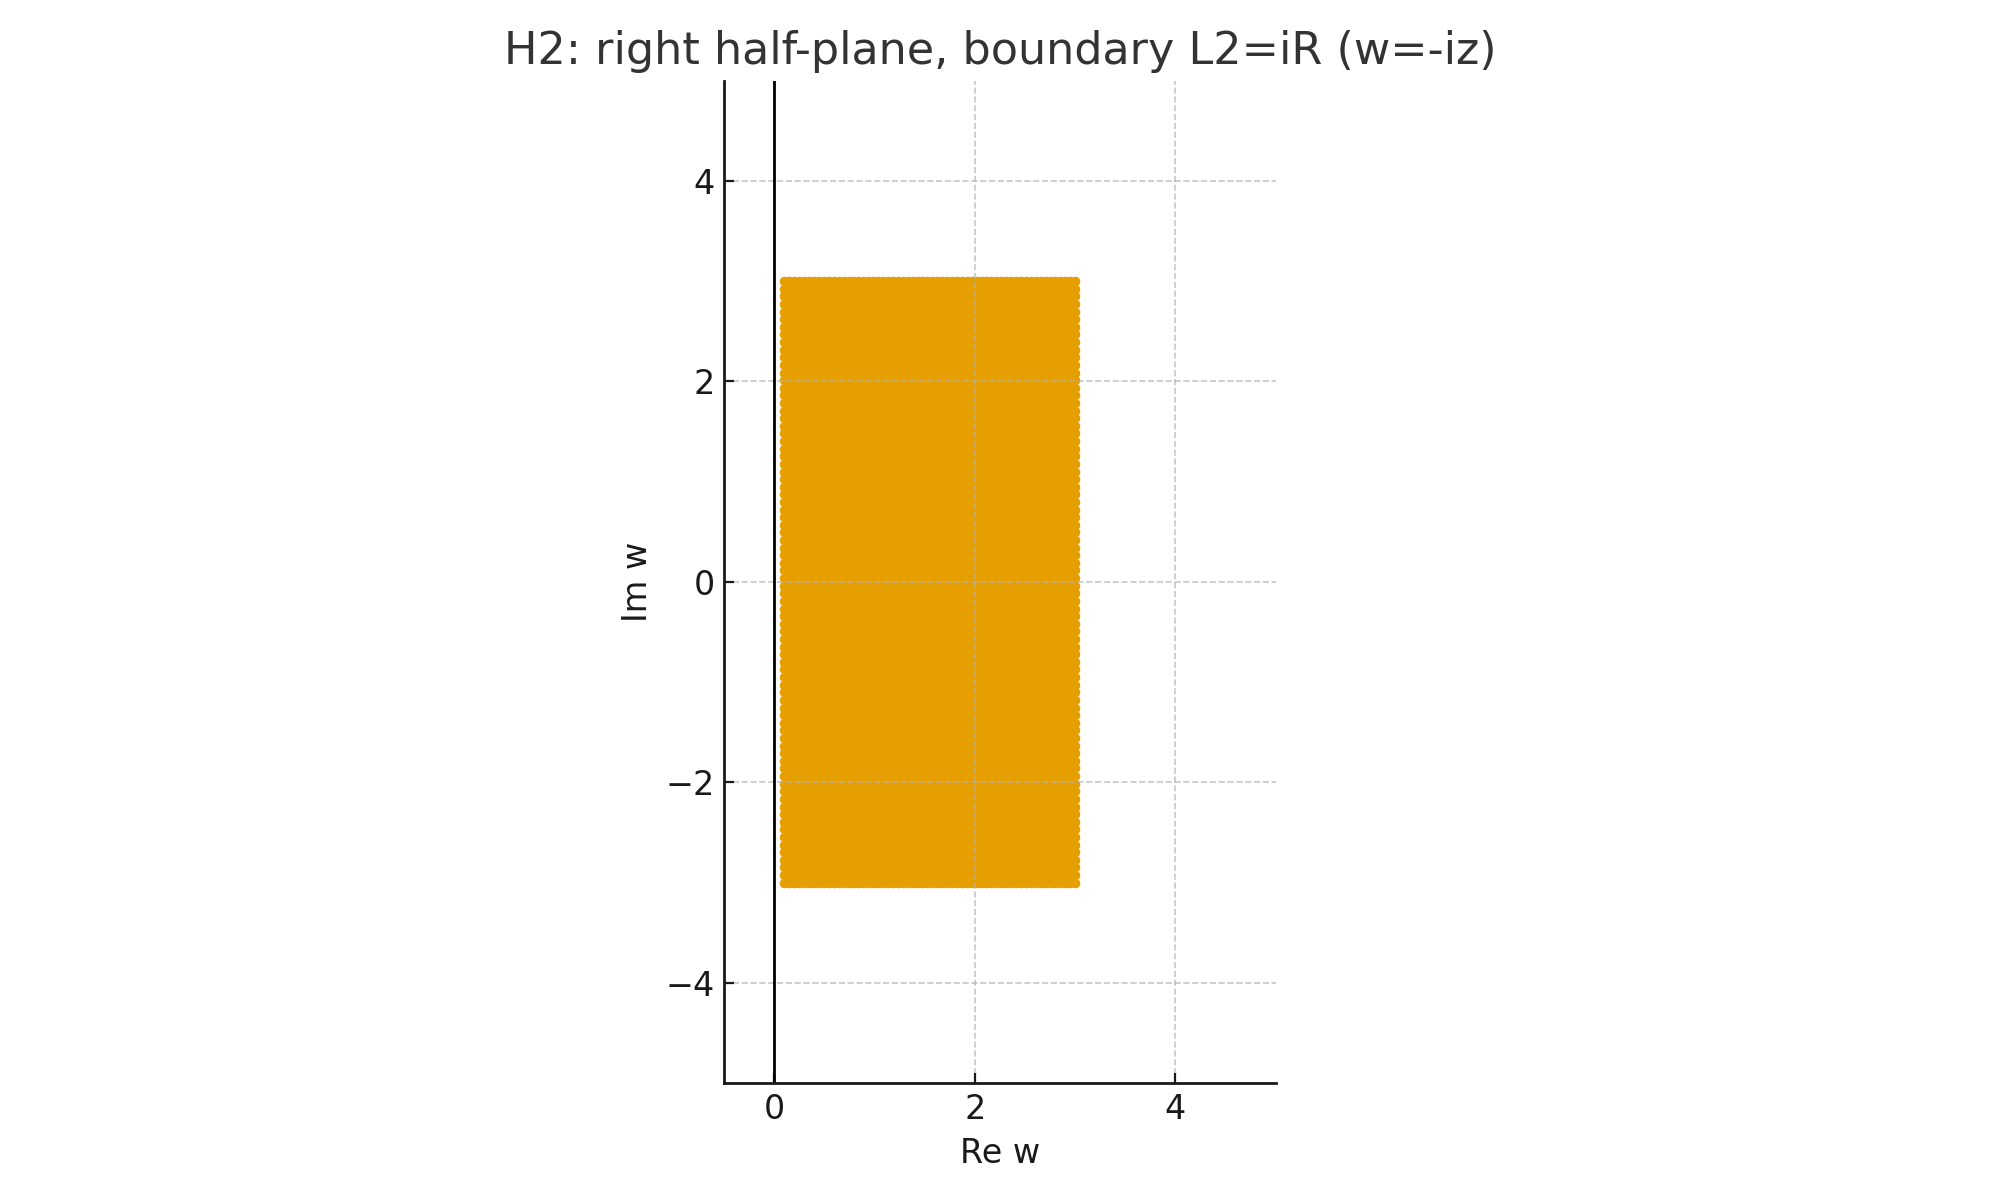
\includegraphics[width=0.78\textwidth]{figures/part04/cp_iv_0065_hp_to_hp_w_plane.png}
  \caption{Source-backed Part IV figure: hp to hp w plane fixed.}
  \label{fig:hp-to-hp-w-plane-fixed}
\end{figure}

\begin{figure}[ht]
  \centering
  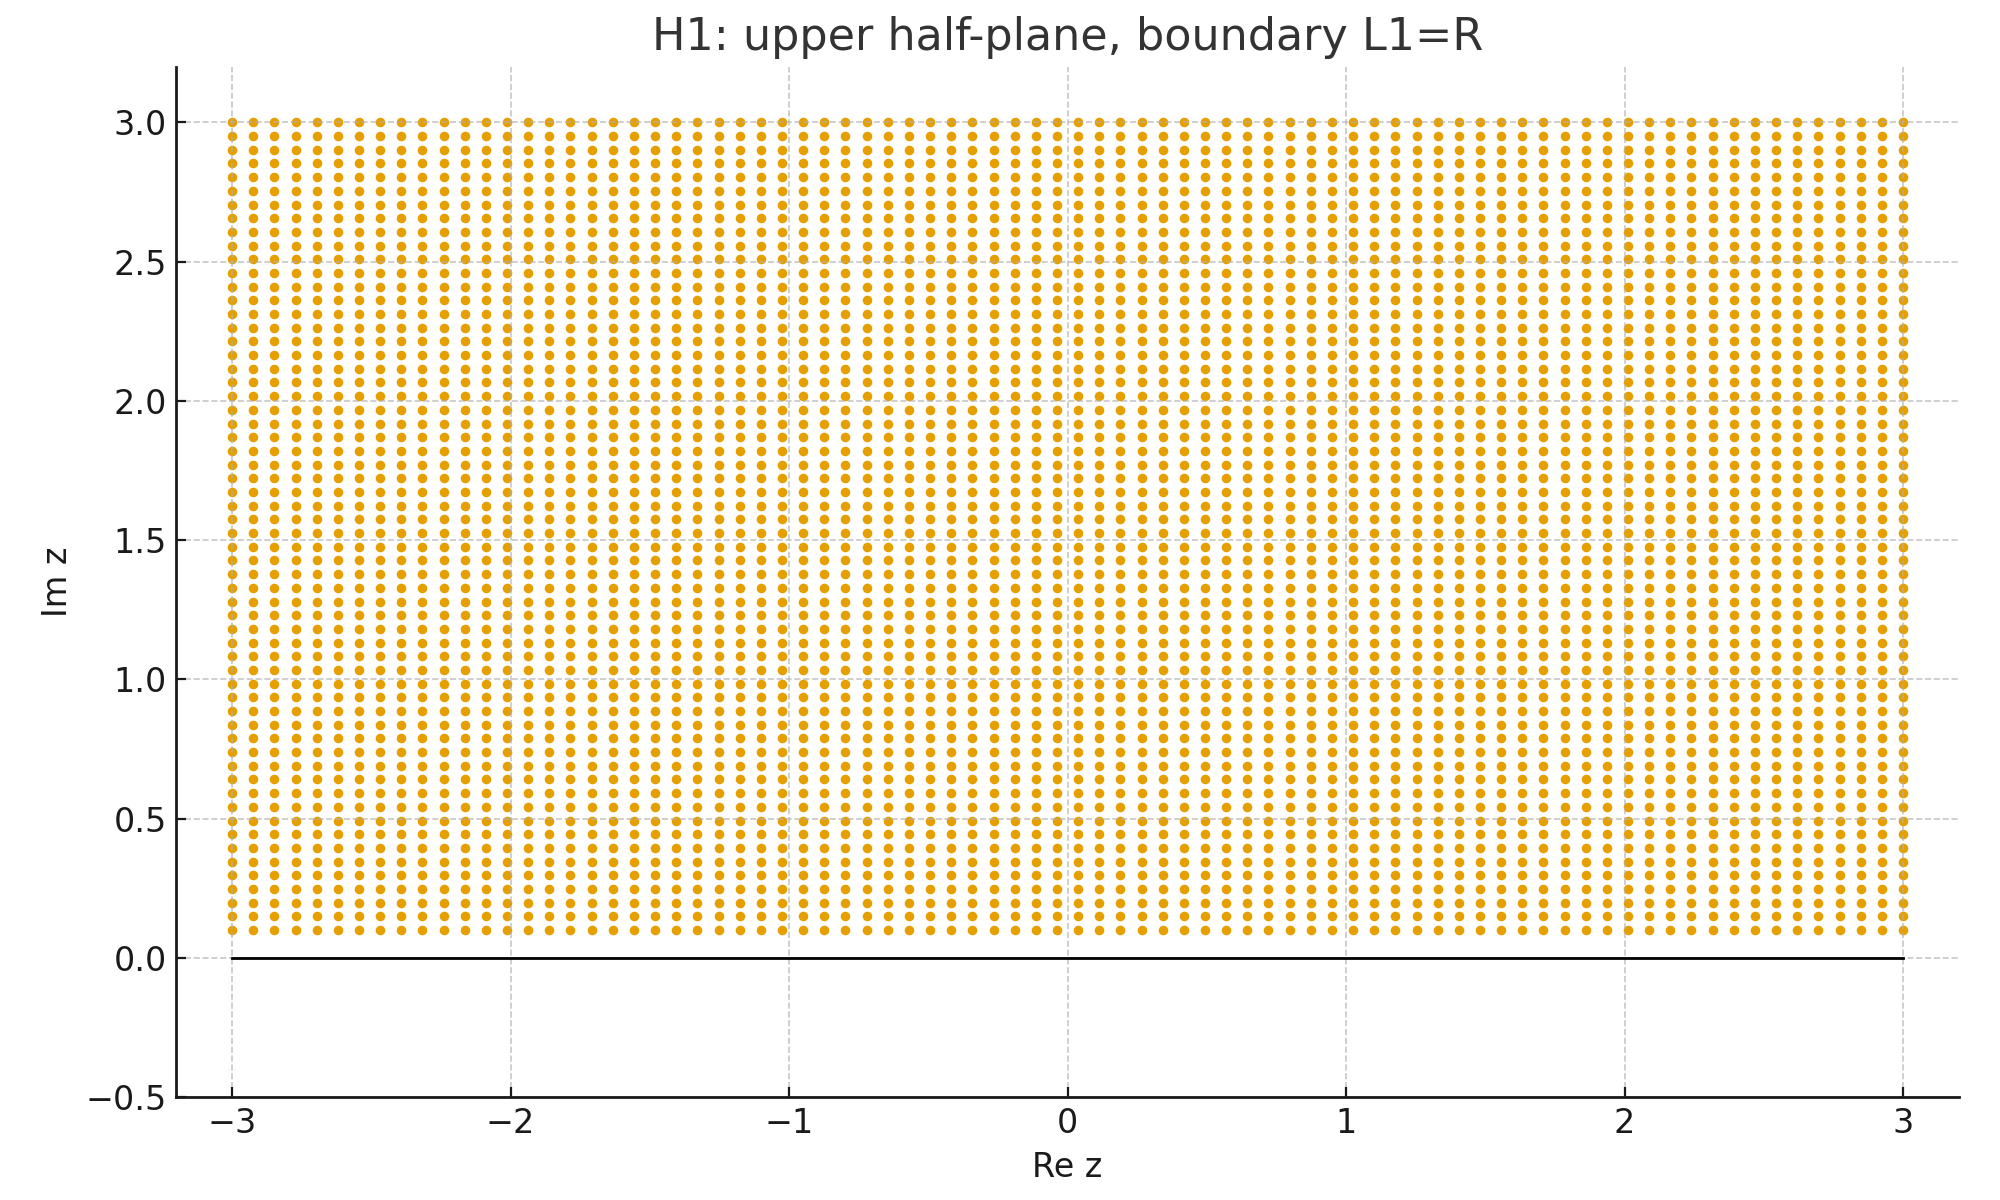
\includegraphics[width=0.78\textwidth]{figures/part04/cp_iv_0065_hp_to_hp_z_plane.png}
  \caption{Source-backed Part IV figure: hp to hp z plane fixed.}
  \label{fig:hp-to-hp-z-plane-fixed}
\end{figure}


\medskip
\noindent
The above example is the simplest possible case of a half-plane to
half-plane mapping, since $T(z)=-iz$ is just a rotation by $-\pi/2$.
However, every biholomorphic map between half-planes can be obtained from
the general three–boundary–points construction described earlier.  In
particular, if $a,b,c$ are three distinct points on the boundary line
$L_1=\mathbb R$, and $A,B,C$ are three distinct points on the boundary
line $L_2=i\mathbb R$ in the same cyclic order, then the unique M\"obius
map satisfying
\[
T(a)=A,\qquad T(b)=B,\qquad T(c)=C
\]
is given explicitly by
\[
T(z)
= \frac{A(C-B) - \Phi(z)\, B(C-A)}{(C-B) - \Phi(z)\,(C-A)},
\qquad
\Phi(z) = \frac{(z-a)(c-b)}{(z-b)(c-a)}.
\]
This expression reduces to $T(z)=-iz$ precisely when the triples
$(a,b,c)$ and $(A,B,C)$ are chosen so that the cross-ratios coincide and
the real axis is mapped to the imaginary axis by a pure rotation.
Thus the simple rotation $T(z)=-iz$ is not an isolated coincidence, but
a special case of the general boundary-normalization principle.

We now give a non-trivial instance of the general construction.
Take three distinct boundary points on the real axis
\[
a=-2,\qquad b=1,\qquad c=4,
\]
and three distinct boundary points on the imaginary axis
\[
A=-i,\qquad B=0,\qquad C=2i,
\]
listed in the same cyclic order (bottom $\to$ top).

The cross-ratio map sending $a,b,c$ to $0,\infty,1$ is
\[
\Phi(z)
= \frac{(z-a)(c-b)}{(z-b)(c-a)}
= \frac{(z+2)(3)}{(z-1)(6)}.
\]

The inverse map sending $0,\infty,1$ back to $A,B,C$ is
\[
\Psi^{-1}(\xi)
= \frac{A(C-B) - \xi\,B(C-A)}{(C-B) - \xi\,(C-A)}.
\]

Hence the desired half-plane map is
\[
T(z) = \Psi^{-1}(\Phi(z)),
\]
which explicitly is
\[
T(z)
= \frac{-i(2i-0) - \Phi(z)\,0(2i - (-i))}
{(2i-0) - \Phi(z)(2i - (-i))}
= \frac{-2i^2}{2i - 3i\,\Phi(z)}
= \frac{2}{\,2i - 3i\,\Phi(z)\,}.
\]

With these boundary triples one verifies
\[
T(a)=A,\qquad T(b)=B,\qquad T(c)=C,
\]
and $T$ maps the chosen side $\Im z>0$ biholomorphically onto the
chosen side $\Re w>0$.

Figures~\ref{fig:nontrivial-hp-z} and \ref{fig:nontrivial-hp-w}
illustrate this map.
\begin{figure}[ht]
  \centering
  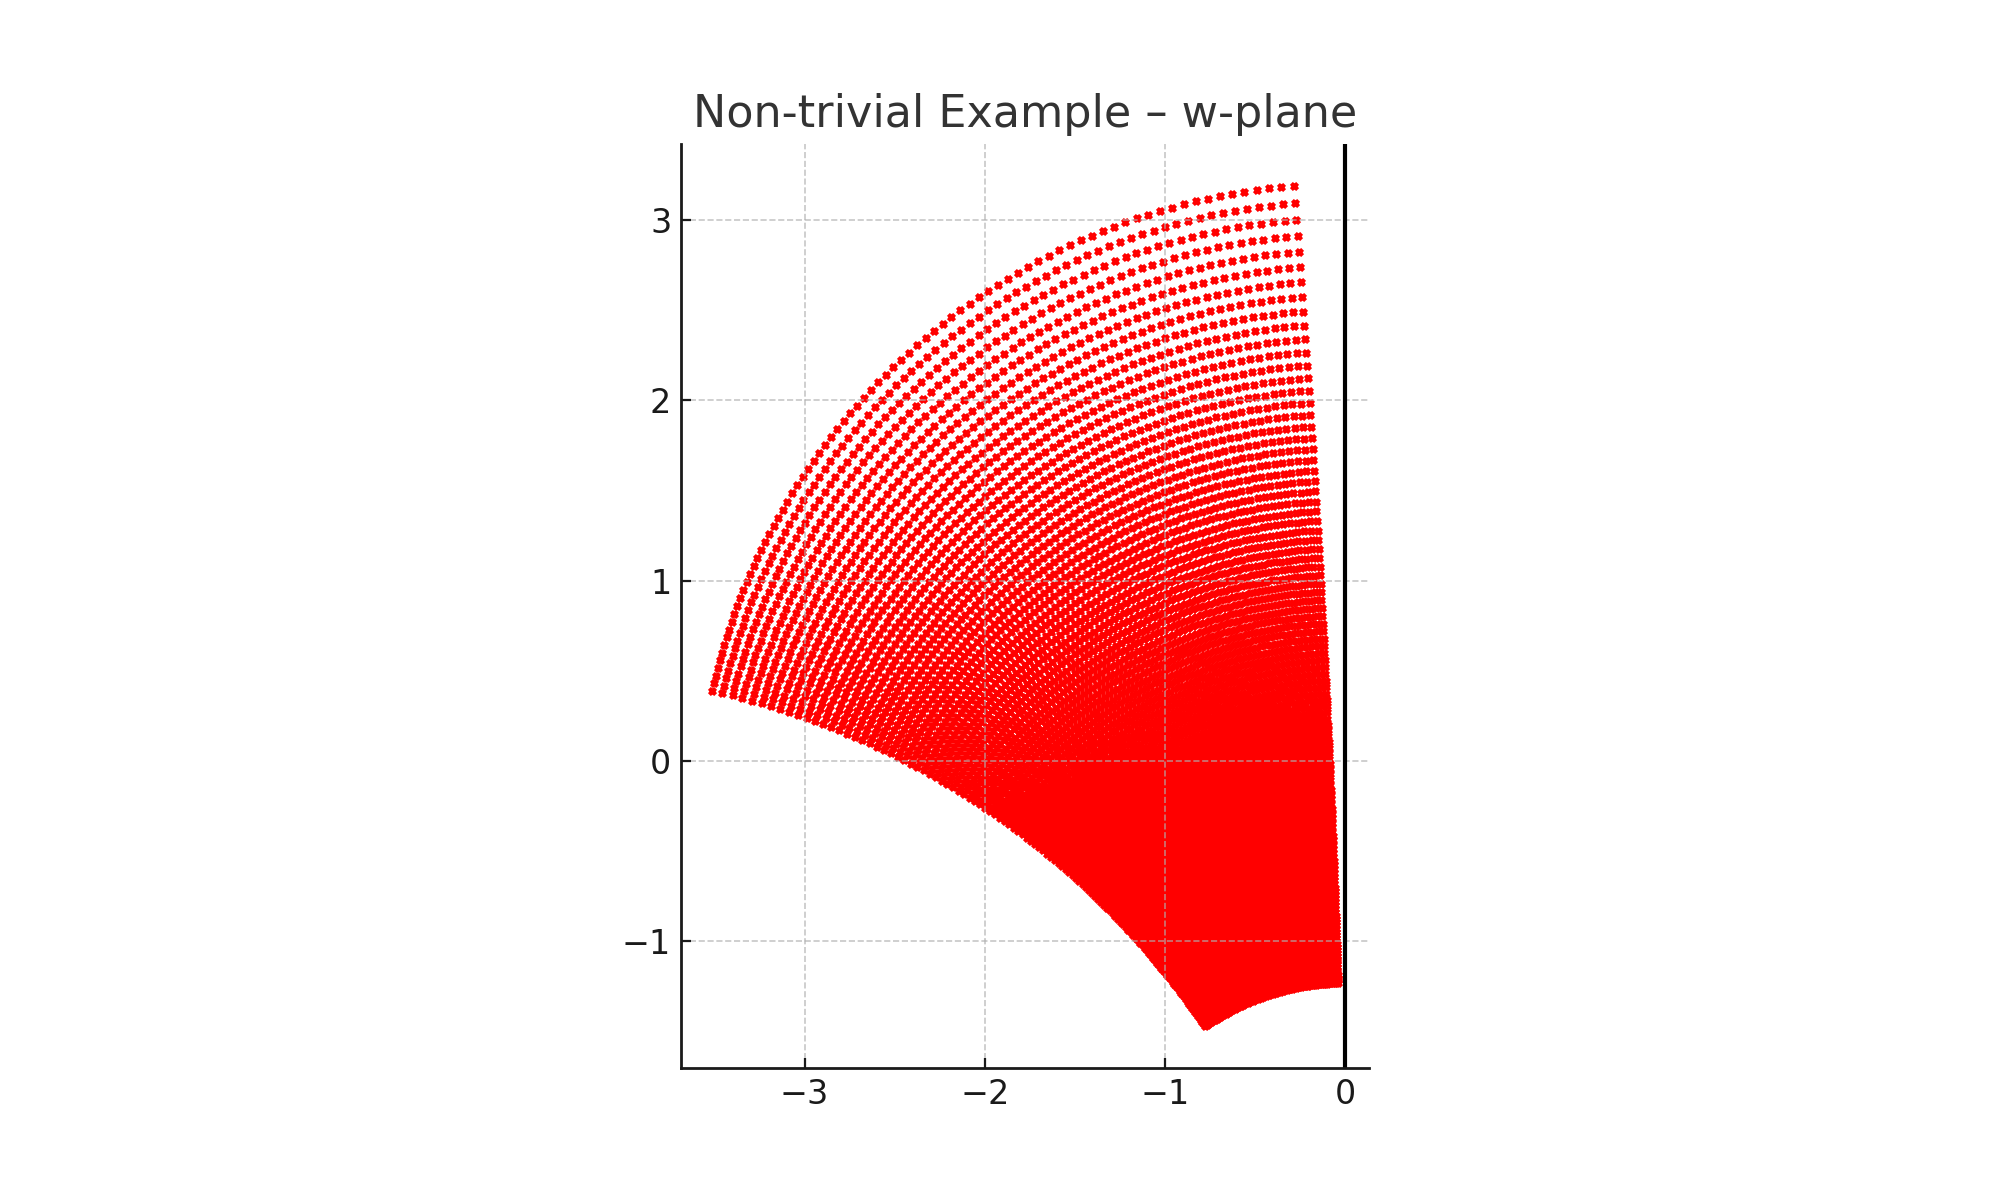
\includegraphics[width=0.78\textwidth]{figures/part04/cp_iv_0065_nontrivial_hp_w_plane.png}
  \caption{Source-backed Part IV figure: nontrivial hp w.}
  \label{fig:nontrivial-hp-w}
\end{figure}

\begin{figure}[ht]
  \centering
  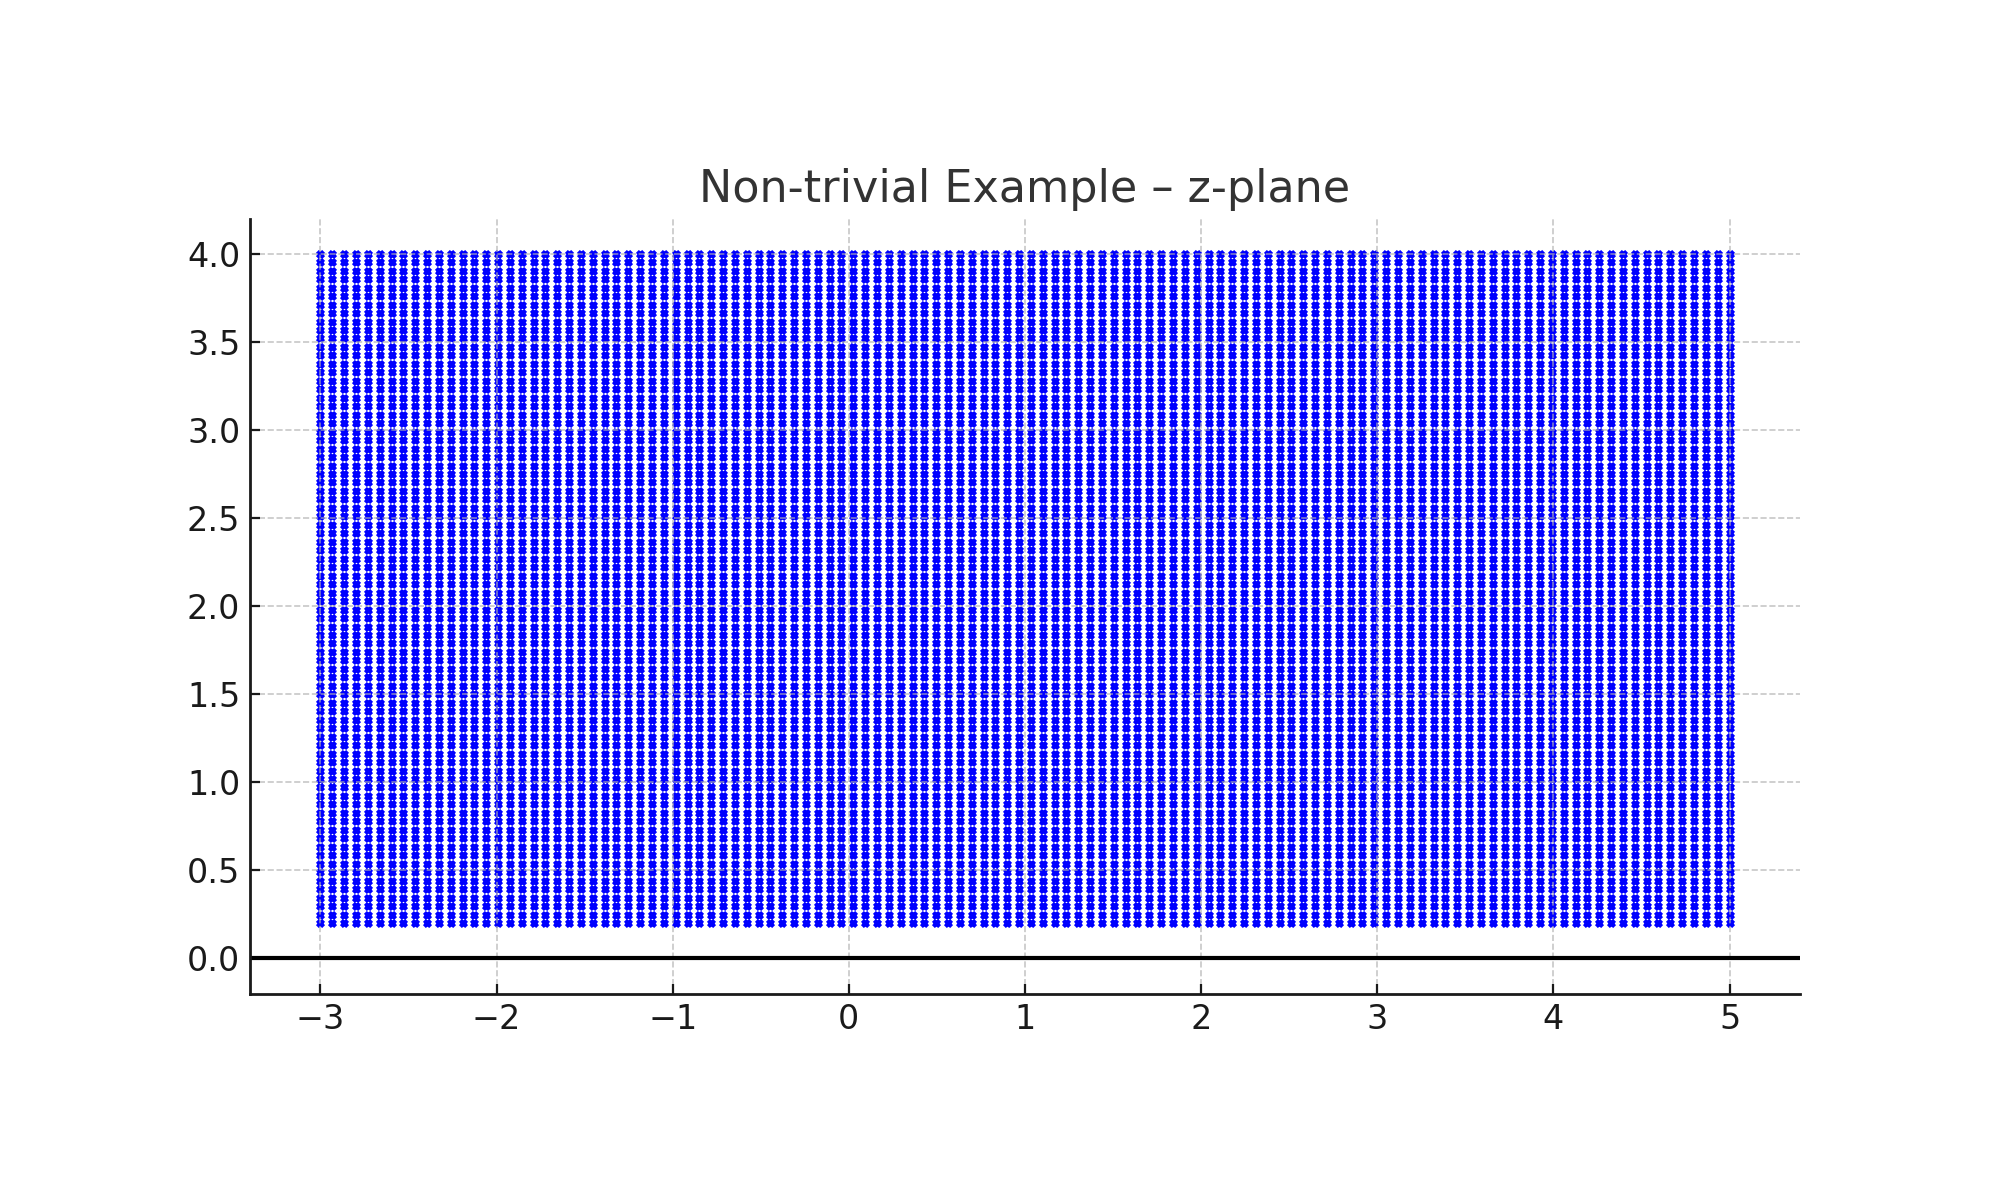
\includegraphics[width=0.78\textwidth]{figures/part04/cp_iv_0065_nontrivial_hp_z_plane.png}
  \caption{Source-backed Part IV figure: nontrivial hp z.}
  \label{fig:nontrivial-hp-z}
\end{figure}


\clearpage
\end{problem}

\begin{solution}
For the elementary map
\[
T(z)=-iz
\]
we have, for \(z=x+iy\),
\[
T(z)=y-ix,
\qquad
\Re T(z)=y.
\]
Therefore
\[
\Im z>0
\iff
\Re T(z)>0,
\]
so \(T\) maps the upper half-plane biholomorphically onto the right half-plane. The real axis is sent to the imaginary axis.

The general three-boundary-point construction is obtained by normalizing both boundary lines. Given
\[
a,b,c\in L_1,\qquad A,B,C\in L_2,
\]
define
\[
\Phi(z)=\frac{(z-a)(c-b)}{(z-b)(c-a)},
\qquad
\Psi(w)=\frac{(w-A)(C-B)}{(w-B)(C-A)}.
\]
Both send the chosen triples to \(0,\infty,1\). Hence
\[
T=\Psi^{-1}\circ\Phi
\]
is the unique M\"obius transformation carrying
\[
a\mapsto A,\qquad b\mapsto B,\qquad c\mapsto C.
\]
If the triples are listed in compatible cyclic order, the chosen half-plane bounded by \(L_1\) is carried to the chosen half-plane bounded by \(L_2\).

For the sample triples
\[
a=-2,\ b=1,\ c=4,
\qquad
A=-i,\ B=0,\ C=2i,
\]
we have
\[
\Phi(z)=\frac{z+2}{2(z-1)}
\]
and
\[
T(z)=\frac{2}{2i-3i\,\Phi(z)}.
\]
Substitution gives
\[
T(-2)=-i,\qquad T(1)=0,\qquad T(4)=2i,
\]
which verifies the normalization.
\end{solution}


\begin{problem}[CP-IV-0066]
\label{prob:cp-iv-0066}
\par\noindent\textbullet\quad Always: $a,z,z^{*}$ are collinear and $|z-a|\cdot|z^{*}-a|=r^2$.

\paragraph{\textbf{TikZ diagram (schematic).}}
\begin{center}

\end{center}

\subsection*{\textbf{Geometric inversion vs holomorphic inversion (modulus inverted; angle preserved vs negated)}}

\paragraph{\textbf{Two maps that are both called “inversion”.}}
Fix a circle $C=\{|z-a|=r\}$.
\end{problem}

\begin{solution}
For geometric inversion in the circle
\[
C=\{z:|z-a|=r\},
\]
the inverse point of \(z\neq a\) is
\[
z^*
=
a+\frac{r^2}{\overline{z-a}}.
\]
Write
\[
z-a=\rho e^{i\theta}.
\]
Then
\[
z^*-a
=
\frac{r^2}{\rho}e^{i\theta}.
\]
Thus \(z-a\) and \(z^*-a\) have the same argument, so \(a,z,z^*\) are collinear and lie on the same ray from \(a\). Moreover,
\[
|z-a|\,|z^*-a|
=
\rho\frac{r^2}{\rho}
=
r^2.
\]
This proves the defining metric relation for circle inversion.

By contrast, the holomorphic map
\[
J_{a,r}(z)=a+\frac{r^2}{z-a}
\]
satisfies
\[
J_{a,r}(z)-a=\frac{r^2}{\rho}e^{-i\theta},
\]
so it inverts the modulus but reverses the angular coordinate. Hence geometric inversion is antiholomorphic, while \(J_{a,r}\) is a M\"obius transformation.
\end{solution}


\begin{problem}[CP-IV-0069]
\label{prob:cp-iv-0069}
\par\noindent\textbullet\quad For \textbf{holomorphic inversion}:
	\[
	J_{a,r}(z)-a=\frac{r^{2}}{\rho e^{i\theta}}
	=\frac{r^{2}}{\rho}\,e^{-i\theta}.
	\]
	Hence
	\[
	|J_{a,r}(z)-a|=\frac{r^{2}}{|z-a|},\qquad
	\arg\bigl(J_{a,r}(z)-a\bigr)=-\arg(z-a)=-\theta.
	\]
	So the \textbf{modulus is inverted} and the \textbf{argument is negated}.

\paragraph{\textbf{Relation between them: “reflection + geometric inversion”.}}
Define reflection across the line through $a$ parallel to the real axis:
\[
R_a(z)=a+\overline{z-a}.
\]
Then
\[
J_{a,r}=R_a\circ I_{a,r}.
\]
Indeed, for $z\neq a$,
\[
(R_a\circ I_{a,r})(z)
=a+\overline{\,I_{a,r}(z)-a\,}
=a+\overline{\frac{r^{2}}{\overline{z-a}}}
=a+\frac{r^{2}}{z-a}
=J_{a,r}(z).
\]

\subsection*{\textbf{Chart: angle preserved vs negated (picture for $a=0$, $r=1$)}}

\paragraph{\textbf{Setup.}}
For the diagram we take $a=0$, $r=1$. (The general case is obtained by translating by $a$ and scaling by $r$.)

\paragraph{\textbf{Interpretation.}}
If $z=\rho e^{i\theta}$:
\[
I_{0,1}(z)=\frac{1}{\overline{z}}=\frac{1}{\rho}e^{i\theta}
\quad\text{(same ray, angle $\theta$),}\qquad
J_{0,1}(z)=\frac{1}{z}=\frac{1}{\rho}e^{-i\theta}
\quad\text{(reflected ray, angle $-\theta$).}
\]

\begin{center}

\end{center}

\subsection*{\textbf{Three common “inversions” in complex analysis and geometry}}

\paragraph{\textbf{(A) The basic Möbius inversion (unit-circle inversion).}}
\[
J(z)=\frac{1}{z}\qquad (z\neq 0).
\]
If $z=\rho e^{i\theta}$, then
\[
J(z)=\frac{1}{\rho}e^{-i\theta},
\qquad
|J(z)|=\frac{1}{|z|},\qquad \arg J(z)=-\arg z.
\]
It fixes the unit circle: if $|z|=1$ then $|J(z)|=1$.

\paragraph{\textbf{(B) Geometric inversion in the circle $|z-a|=r$ (anti-holomorphic).}}
\[
I_{a,r}(z)=a+\frac{r^{2}}{\overline{z-a}}\qquad (z\neq a).
\]
Write $z-a=\rho e^{i\theta}$, then
\[
I_{a,r}(z)-a=\frac{r^{2}}{\rho}e^{i\theta},
\qquad
|I_{a,r}(z)-a|=\frac{r^{2}}{|z-a|},\qquad
\arg\bigl(I_{a,r}(z)-a\bigr)=\arg(z-a).
\]
Thus it inverts the radius but \emph{preserves} the argument (same ray from $a$). It fixes the circle $|z-a|=r$ pointwise.

\paragraph{\textbf{(C) Holomorphic “circle inversion” (a Möbius map).}}
\[
H_{a,r}(z)=a+\frac{r^{2}}{z-a}\qquad (z\neq a).
\]
Write $z-a=\rho e^{i\theta}$, then
\[
H_{a,r}(z)-a=\frac{r^{2}}{\rho}e^{-i\theta},
\qquad
|H_{a,r}(z)-a|=\frac{r^{2}}{|z-a|},\qquad
\arg\bigl(H_{a,r}(z)-a\bigr)=-\arg(z-a).
\]
Thus it inverts the radius and \emph{negates} the argument (reflection of the ray). It preserves the circle $|z-a|=r$ as a set (not pointwise).

\paragraph{\textbf{Relationship between (B) and (C).}}
Let
\[
R_a(z)=a+\overline{z-a}
\]
be reflection across the horizontal line through $a$. Then
\[
H_{a,r}=R_a\circ I_{a,r}.
\]

\subsection*{\textbf{Summary table}}

\begin{center}
	\renewcommand{\arraystretch}{1.25}
	\begin{tabular}{|l|l|l|l|}
		\hline
		\textbf{Name} & \textbf{Formula} & \textbf{Modulus rule} & \textbf{Angle rule} \\
		\hline
		Unit Möbius inversion & $J(z)=\dfrac1z$ &
		$\left|J(z)\right|=\dfrac{1}{|z|}$ &
		$\arg J(z)= -\arg z$ \\
		\hline
		Geometric circle inversion & $I_{a,r}(z)=a+\dfrac{r^2}{\overline{z-a}}$ &
		$\left|I_{a,r}(z)-a\right|=\dfrac{r^2}{|z-a|}$ &
		$\arg(I_{a,r}(z)-a)=\arg(z-a)$ \\
		\hline
		Holomorphic circle inversion & $H_{a,r}(z)=a+\dfrac{r^2}{z-a}$ &
		$\left|H_{a,r}(z)-a\right|=\dfrac{r^2}{|z-a|}$ &
		$\arg(H_{a,r}(z)-a)= -\arg(z-a)$ \\
		\hline
	\end{tabular}
\end{center}

	\subsection*{\textbf{Inversion as a Möbius transformation (and its geometric cousin)}}

	\paragraph{\textbf{Möbius transformations.}}
	A Möbius map is
	\[
	f(z)=\frac{Az+B}{Cz+D},\qquad AD-BC\neq 0,
	\]
	and it is represented (projectively) by the matrix
	\[
	\begin{pmatrix}A & B\\ C & D\end{pmatrix}
	\quad\text{in } PSL(2,\mathbb C).
	\]

	\subsection*{\textbf{1) Where is the simple inversion $1/z$ in Möbius form?}}
	Take
	\[
	f(z)=\frac{0\cdot z+1}{1\cdot z+0}=\frac{1}{z}.
	\]
	So $1/z$ corresponds to the matrix
	\[
	\begin{pmatrix}0 & 1\\ 1 & 0\end{pmatrix}
	\quad\text{(in } PSL(2,\mathbb C)\text{).}
	\]

	\subsection*{\textbf{2) Where is the “radius-$r$” holomorphic inversion $r^{2}/z$?}}
	Just scale:
	\[
	f(z)=\frac{0\cdot z+r^{2}}{1\cdot z+0}=\frac{r^{2}}{z},
	\qquad
	\begin{pmatrix}0 & r^{2}\\ 1 & 0\end{pmatrix}.
	\]

	\subsection*{\textbf{3) Where is the shifted version $a+\dfrac{r^{2}}{z-a}$?}}

	\paragraph{\textbf{Conjugation by translations.}}
	Let $T_a(z)=z+a$. Starting from $r^{2}/z$ we obtain
	\[
	H_{a,r}(z)=a+\frac{r^{2}}{z-a}
	= T_a\circ\left(\frac{r^{2}}{z}\right)\circ T_{-a}(z).
	\]

	\paragraph{\textbf{As an explicit fraction $(Az+B)/(Cz+D)$.}}
	Compute:
	\[
	H_{a,r}(z)=a+\frac{r^{2}}{z-a}
	=\frac{a(z-a)+r^{2}}{z-a}
	=\frac{az+(r^{2}-a^{2})}{z-a}.
	\]
	Therefore, matching with $\dfrac{Az+B}{Cz+D}$, we read off
	\[
	A=a,\qquad B=r^{2}-a^{2},\qquad C=1,\qquad D=-a,
	\]
	and hence
	\[
	H_{a,r}(z)\ \longleftrightarrow\
	\begin{pmatrix}
		a & r^{2}-a^{2}\\[2pt]
		1 & -a
	\end{pmatrix},
	\qquad
	\det=
	a(-a)-(r^{2}-a^{2})\cdot 1=-r^{2}\neq 0.
	\]

	\subsection*{\textbf{4) What about geometric circle inversion $a+\dfrac{r^{2}}{\overline{z-a}}$?}}

	\paragraph{\textbf{Not Möbius (anti-holomorphic).}}
	The geometric circle inversion is
	\[
	I_{a,r}(z)=a+\frac{r^{2}}{\overline{z-a}},
	\]
	and it is \emph{not} Möbius because it depends on $\overline{z}$ (it is anti-holomorphic).

	\paragraph{\textbf{But it becomes Möbius after composing with a reflection.}}
	Let
	\[
	R_a(z)=a+\overline{z-a}
	\]
	(reflection across the horizontal line through $a$). Then
	\[
	H_{a,r}=R_a\circ I_{a,r}.
	\]

	\subsection*{\textbf{Opposite direction: starting from $(A,B,C,D)$}}

	\paragraph{\textbf{(I) Universal factorization when $C\neq 0$.}}
	Assume $C\neq 0$. Define
	\[
	\alpha=\frac{A}{C},\qquad
	\delta=\frac{D}{C},\qquad
	\beta=\frac{BC-AD}{C^{2}}.
	\]
	Then the identity
	\[
	\frac{Az+B}{Cz+D}=\alpha+\frac{\beta}{z+\delta}
	\]
	holds. Consequently,
	\[
	f=T_{\alpha}\circ S_{\beta}\circ J\circ T_{\delta},
	\qquad
	T_t(z)=z+t,\quad S_\lambda(z)=\lambda z,\quad J(z)=\frac{1}{z}.
	\]

	\paragraph{\textbf{(II) The affine case $C=0$.}}
	If $C=0$, then
	\[
	f(z)=\frac{Az+B}{D}=\left(\frac{A}{D}\right)z+\left(\frac{B}{D}\right),
	\]
	so $f$ is just a similarity plus a translation.

	\paragraph{\textbf{(III) When is $f$ of the special form $H_{a,r}(z)=a+\dfrac{r^{2}}{z-a}$?}}
	Assume $C\neq 0$. The map $f(z)=\dfrac{Az+B}{Cz+D}$ is of the form
	\[
	H_{a,r}(z)=a+\frac{r^{2}}{z-a}
	\]
	(up to an overall nonzero scalar in the coefficients) exactly when
	\[
	A=-D.
	\]
	In that case one can set
	\[
	a=\frac{A}{C}=-\frac{D}{C},
	\qquad
	r^{2}=\frac{BC-AD}{C^{2}},
	\]
	and then indeed
	\[
	\frac{Az+B}{Cz+D}=a+\frac{r^{2}}{z-a}.
	\]

	\subsection*{\textbf{How this relates to the exercise: why (i) $\Rightarrow$ (ii)}}

	\paragraph{\textbf{Goal of (ii).}}
	We want to prove: every Möbius map
	\[
	f(z)=\frac{Az+B}{Cz+D}\qquad(AD-BC\neq 0)
	\]
	is a composition of inversions (in circles/lines).

	\paragraph{\textbf{Step 1: (i) provides the explicit inversion map.}}
	From (i), inversion in the circle $|z-a|=r$ is the map
	\[
	I_{a,r}(z)=a+\frac{r^{2}}{\overline{z-a}}.
	\]
	This is a genuine Euclidean circle inversion: it sends $z$ to the unique point $z^{*}$ on the ray from $a$ through $z$
	such that $|z-a|\cdot|z^{*}-a|=r^{2}$.

	\paragraph{\textbf{Step 2: reduce an arbitrary Möbius map to generators.}}
	If $C\neq 0$, define
	\[
	\alpha=\frac{A}{C},\qquad
	\delta=\frac{D}{C},\qquad
	\beta=\frac{BC-AD}{C^{2}}.
	\]
	Then one checks the identity
	\[
	\frac{Az+B}{Cz+D}=\alpha+\frac{\beta}{z+\delta}.
	\]
	Hence, writing
	\[
	T_t(z)=z+t,\qquad S_\lambda(z)=\lambda z,\qquad J(z)=\frac{1}{z},
	\]
	we obtain the factorization
	\[
	f \;=\; T_{\alpha}\circ S_{\beta}\circ J\circ T_{\delta}.
	\]
	If $C=0$, then $f(z)=\left(\frac{A}{D}\right)z+\left(\frac{B}{D}\right)$ is already a similarity plus translation.

	\paragraph{\textbf{Step 3: realize each generator as a composition of inversions.}}
	We allow inversions in circles and also in lines (lines are circles through $\infty$, i.e.\ reflections).
\end{problem}

\begin{solution}
Let
\[
I_{a,r}(z)=a+\frac{r^2}{\overline{z-a}}
\]
denote geometric inversion and
\[
H_{a,r}(z)=a+\frac{r^2}{z-a}
\]
the holomorphic inversion. If \(z-a=\rho e^{i\theta}\), then
\[
I_{a,r}(z)-a=\frac{r^2}{\rho}e^{i\theta},
\qquad
H_{a,r}(z)-a=\frac{r^2}{\rho}e^{-i\theta}.
\]
Thus both invert the radius, but geometric inversion preserves the ray while holomorphic inversion reflects the angle.

Let
\[
R_a(z)=a+\overline{z-a}.
\]
Then
\[
R_a(I_{a,r}(z))
=
a+\overline{\frac{r^2}{\overline{z-a}}}
=
a+\frac{r^2}{z-a}
=
H_{a,r}(z).
\]
Therefore
\[
H_{a,r}=R_a\circ I_{a,r}.
\]

The holomorphic inversion is M\"obius:
\[
H_{a,r}(z)
=
\frac{az+(r^2-a^2)}{z-a},
\]
with representing matrix
\[
\begin{pmatrix}
a&r^2-a^2\\
1&-a
\end{pmatrix},
\]
whose determinant is \(-r^2\neq0\).

Conversely, if
\[
f(z)=\frac{Az+B}{Cz+D},
\qquad C\neq0,
\]
then
\[
f(z)
=
\frac AC
+
\frac{BC-AD}{C^2}\,
\frac{1}{z+D/C}.
\]
Hence every M\"obius transformation is built from translations, a nonzero complex scaling, and the basic inversion \(z\mapsto1/z\). Since reflections and similarities themselves can be realized by compositions of line/circle inversions, this gives the standard generation of M\"obius transformations by inversions.
\end{solution}


\begin{problem}[CP-IV-0072]
\label{prob:cp-iv-0072}
(i) Let $f:U\to\mathbb C$ be holomorphic on a domain $U$. Show that $f$ is constant if any one of its real part, modulus, or argument is constant.\\
(ii) Find all entire functions of the form $f(x+iy)=u(x)+i\,v(y)$ with $u,v$ real-valued.\\
(iii) Find all entire functions whose real part is $x^3-3xy^2$.
\end{problem}

\begin{solution}
\emph{(i) One part constant $\Rightarrow$ $f$ constant.}
Write $f=u+iv$.
If $\Re f=u$ is constant, then $u_x=u_y=0$; the CR equations $u_x=v_y$, $u_y=-v_x$ give $v_x=v_y=0$, hence $f$ is constant.

If $|f|$ is constant, either $f\equiv0$ or $f(U)$ lies on a circle, which is not open; by the Open Mapping Theorem, $f$ must be constant.
(Alternatively: for holomorphic $f$, $f_x=f'$ and $f_y=i f'$, so from $|f|^2$ constant
$0=\partial_x|f|^2=2\Re(f'\bar f)$ and $0=\partial_y|f|^2=-2\Im(f'\bar f)$, hence $f'\bar f=0$, so $f'\equiv0$ and $f$ is constant.)

If $\arg f$ is constant, $f(U)$ lies on a ray, not open; the Open Mapping Theorem again forces $f$ to be constant.

\medskip
\emph{(ii) Form $u(x)+i v(y)$.}
Here $u_y=0$ and $v_x=0$. CR yields $u_x=v_y=:c$ (a real constant). Hence
$u(x)=cx+a$, $v(y)=cy+b$ with $a,b\in\mathbb R$, $c\in\mathbb R$, and
\[
f(z)=u(x)+i v(y)=(a+ib)+c(x+iy)=(a+ib)+c\,z.
\]
Thus all such entire functions are $f(z)=\alpha + c z$ with $\alpha\in\mathbb C$ and $c\in\mathbb R$.

\medskip
\emph{(iii) Prescribed real part $x^3-3xy^2$.}
Since $\Re(z^3)=x^3-3xy^2$, any entire $f$ with this real part satisfies $f-z^3$ has zero real part and hence is a purely imaginary constant. Therefore
\[
\boxed{\,f(z)=z^3+i\beta,\quad \beta\in\mathbb R.\,}
\]
\end{solution}

\begin{problem}[CP-IV-0077]
\label{prob:cp-iv-0077}
(restated).

	\par\noindent\textbullet\quad Let $f$ be entire and satisfy $f(1/n)=1/n$ for all $n\in\mathbb N$. Prove that $f(z)\equiv z$.
	\par\noindent\textbullet\quad Let $f$ be entire and satisfy $f(n)=n^{2}$ for all $n\in\mathbb Z$. Must $f$ equal $z^{2}$? Give a justification or a counterexample.
	\par\noindent\textbullet\quad Let $f$ be holomorphic on $D(0,2)$. Show that there exists $n\in\mathbb N$ with $f(1/n)\ne 1/(n+1)$.

\medskip

\emph{Holomorphic / entire.}
A function $f$ is holomorphic on a domain $U\subset\mathbb C$ if it is complex differentiable at every point of $U$.
It is \emph{entire} if it is holomorphic on all of $\mathbb C$.
A \emph{domain} is a nonempty, open, connected subset of $\mathbb C$.

\medskip
\emph{Accumulation point.}
A sequence $(z_n)\subset U$ has an accumulation point $z_\ast\in U$ if $z_n\to z_\ast$ with $z_n\neq z_\ast$ eventually.

\medskip
\emph{Isolated zeros and the identity theorem.}
If $f$ is holomorphic on $U$ and not identically zero, then its zeros have no accumulation point in $U$.
If $f,g$ are holomorphic on $U$ and $f=g$ on a set with a limit point in $U$ (e.g.\ $z_n\to z_\ast\in U$), then $f\equiv g$ on $U$.
Equivalently, if a holomorphic $f$ vanishes on such a set, then $f\equiv 0$.

\medskip
\emph{An entire function vanishing on $\mathbb Z$.}
$\sin(\pi z)$ is entire and $\sin(\pi n)=0$ for all $n\in\mathbb Z$.
Thus for prescribed integer values, one may add $\sin(\pi z)\cdot H(z)$ (with $H$ entire) without changing those values.

\medskip
\emph{Removable singularities (Riemann).}
If $f$ is holomorphic on $0<|z-a|<r$ and bounded near $a$, then $f$ extends holomorphically to $z=a$.

\medskip
\emph{How these tools are used in Problem 8.}

	\par\noindent\textbullet\quad \textbf{(i)} $g(z)=f(z)-z$ entire with $g(1/n)=0$ and $1/n\to 0\in\mathbb C$ $\Rightarrow$ $g\equiv 0$.
	\par\noindent\textbullet\quad \textbf{(ii)} Integers have no accumulation in $\mathbb C$; non-uniqueness via $\sin(\pi z)$.
	\par\noindent\textbullet\quad \textbf{(iii)} Zeros at $1/n\to 0$ in $D(0,2)\setminus\{-1\}$ force identity with a meromorphic function that has a pole at $-1$ — contradiction.

\medskip
\end{problem}

\begin{solution}
\subsection*{Solution to (1): Existence on $U$}

Because $f$ is holomorphic and nonvanishing, the function
\[
g(z) := \frac{f'(z)}{f(z)}
\]
is holomorphic on $U$. Since $U$ is simply connected, there exists a holomorphic primitive $G$ with $G'=g$ on $U$.

\medskip

Define
\[
H(z) := e^{G(z)} .
\]
Then
\[
\frac{H'(z)}{H(z)} = G'(z) = \frac{f'(z)}{f(z)}
\qquad\Longrightarrow\qquad
\Big(\log\frac{H(z)}{f(z)}\Big)'=0 .
\]
Hence $H/f$ is constant on $U$. Choose $c\in\mathbf{C}$ with $e^{c} = f(z_0)/H(z_0)$ for some (hence every) $z_0\in U$, and set
\[
F(z) := G(z) + c .
\]
Then $e^{F(z)} = f(z)$ on $U$, so $F$ is a holomorphic branch of $\log f$.

\medskip

\noindent\textit{Uniqueness up to $2\pi i\mathbf{Z}$.}
If $F_1$ and $F_2$ both satisfy $e^{F}=f$, then $e^{F_1-F_2}\equiv 1$, so $F_1-F_2$ is a constant of the form $2\pi i\,k$ with $k\in\mathbf{Z}$.

\bigskip\hrule\bigskip
\end{solution}

\begin{problem}[CP-IV-0080]
\label{prob:cp-iv-0080}
\par\noindent\textbullet\quad (\textbf{Schwarz's Lemma}) Let $f$ be analytic on $D(0,1)$ with $|f(z)|\le 1$ and $f(0)=0$.
	Apply the maximum principle to $f(z)/z$ to show $|f(z)|\le |z|$. Show also that if $|f(w)|=|w|$ for some $w\neq 0$, then $f(z)=c\,z$ for some constant $c$.

	\par\noindent\textbullet\quad Use Schwarz's Lemma to prove that any conformal equivalence $\Phi:D(0,1)\to D(0,1)$ is given by a Möbius transformation.

If a holomorphic $g$ on $0<|z|<1$ is bounded near $0$, then $g$ extends holomorphically to $z=0$ (removable singularity).
A non-constant holomorphic function does not attain a maximum of its modulus in the interior (maximum modulus principle).
For $a\in D$, the map $\displaystyle \phi_a(z)=\frac{z-a}{1-\overline a\,z}$ is a biholomorphism $D\to D$ with $\phi_a(a)=0$.
\end{problem}

% Designed Companion Part IV figure
% Intended for \input{...} beside the matching canonical problem.
\begin{figure}[ht]
\centering
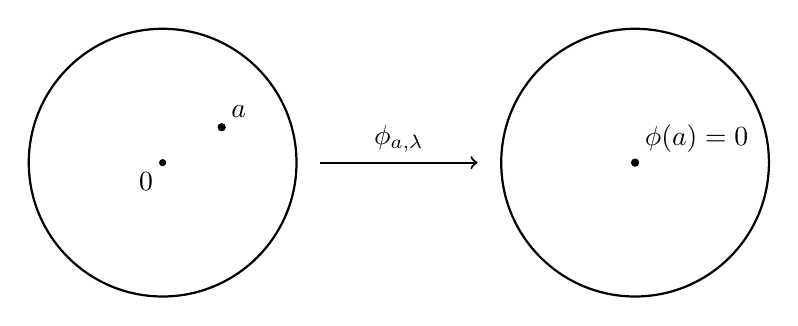
\begin{tikzpicture}[scale=1.0]
  \begin{scope}[xshift=-3.0cm]
    \draw[thick] (0,0) circle (1.7);
    \fill (0.75,0.45) circle (1.5pt) node[above right] {$a$};
    \fill (0,0) circle (1.3pt) node[below left] {$0$};
  \end{scope}
  \draw[->,thick] (-1.0,0)--(1.0,0) node[midway,above] {$\phi_{a,\lambda}$};
  \begin{scope}[xshift=3.0cm]
    \draw[thick] (0,0) circle (1.7);
    \fill (0,0) circle (1.5pt) node[above right] {$\phi(a)=0$};
  \end{scope}
\end{tikzpicture}
\caption{Every conformal automorphism of the disk is a Blaschke factor followed by a rotation: first send $a$ to $0$, then Schwarz's lemma forces the remaining normalized automorphism to be $z\mapsto\lambda z$.}
\label{fig:cp-iv-0080-schwarz-disk-automorphism}
\end{figure}


\begin{solution}
\emph{(i)} Define
\[
g(z)=\begin{cases}
	\dfrac{f(z)}{z},& z\neq 0,\\[4pt]
	f'(0),& z=0.
\end{cases}
\]
Because $|f(z)|\le 1$ and $f(0)=0$, $g$ is bounded near $0$, hence extends holomorphically to $D$.
For $0<r<1$, on $|z|=r$ we have $|g(z)|\le 1/r$. By the maximum modulus principle on each smaller disk, letting $r\uparrow 1$ gives $|g(z)|\le 1$ for all $z\in D$.
Thus $|f(z)|\le |z|$ and $|f'(0)|=|g(0)|\le 1$.

If $|f(w)|=|w|$ for some $w\ne 0$, then $|g(w)|=1$. By the maximum modulus principle $g$ has constant modulus $1$ on $D$, hence $g\equiv c$ with $|c|=1$ and $f(z)=c\,z$.

\medskip
\emph{(ii)} Let $\Phi:D\to D$ be a conformal bijection and set $a=\Phi(0)$. Consider $F=\phi_a\circ \Phi$, where $\displaystyle \phi_a(z)=\frac{z-a}{1-\overline a\,z}$.
Then $F:D\to D$ is holomorphic with $F(0)=0$. By Schwarz's Lemma, $F(z)=\lambda z$ with $|\lambda|\le 1$; since $\Phi$ is bijective, $| \lambda|=1$.
Therefore
\[
\Phi(z)=\phi_a^{-1}(\lambda z)=\lambda\,\frac{z-a}{1-\overline a\,z},
\]
a Möbius automorphism of the disk.
\end{solution}

\begin{problem}[CP-IV-0082]
\label{prob:cp-iv-0082}
Associated family in Weierstrass data (local isometry)

\paragraph{\textbf{Problem statement.}}
The Weierstrass representation is not unique: if $\phi_{(f,g)}:D\to\mathbb{R}^3$ is the associated parametrization and
$\alpha:W\to D$ is a bijective holomorphic map, then $\phi_{(f,g)}\circ\alpha$ is another representation of the same minimal
surface and it must have the same form with different $f$ and $g$ (which should be specified).
By choosing $\alpha(z)=g^{-1}(z)$, show that, locally around regular points of $g$ (where $g'\neq 0$), we can assume
that our pair $(f,g)$ is of the form $(F,\mathrm{id})$, for some local holomorphic function $F$. We denote such a
representation by $\phi_F$. Show that the minimal surfaces given by $\phi_{e^{-i\theta}F}$ for $\theta\in\mathbb{R}$
are all locally isometric.

\medskip

We use the Weierstrass data $(f,g)$ (holomorphic on $D$, with $g$ meromorphic in general) in the form
\[
\phi_{(f,g)}(z)
=
\Re\int^z
\Bigl(\tfrac12 f(1-g^2),\ \tfrac{i}{2}f(1+g^2),\ fg\Bigr)\,dz.
\]
Its induced metric is
\[
ds^2
=
\frac{|f|^2(1+|g|^2)^2}{4}\,|dz|^2.
\]

\medskip
\end{problem}

% Designed Companion Part IV figure
% Intended for \input{...} beside the matching canonical problem.
\begin{figure}[ht]
\centering
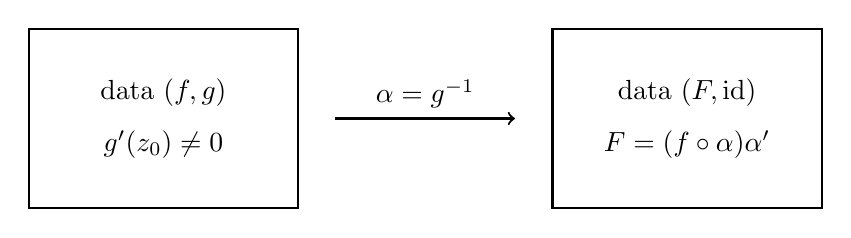
\begin{tikzpicture}[scale=0.95]
  \begin{scope}[xshift=-3.5cm]
    \draw[thick] (-1.8,-1.2) rectangle (1.8,1.2);
    \node at (0,0.35) {data $(f,g)$};
    \node at (0,-0.35) {$g'(z_0)\ne0$};
  \end{scope}
  \draw[->,thick] (-1.2,0)--(1.2,0) node[midway,above] {$\alpha=g^{-1}$};
  \begin{scope}[xshift=3.5cm]
    \draw[thick] (-1.8,-1.2) rectangle (1.8,1.2);
    \node at (0,0.35) {data $(F,\mathrm{id})$};
    \node at (0,-0.35) {$F=(f\circ\alpha)\alpha'$};
  \end{scope}
\end{tikzpicture}
\caption{At a regular point of the Gauss map, $g$ is locally invertible. Reparametrizing by $\alpha=g^{-1}$ changes the Weierstrass data to $(F,\mathrm{id})$, making the Gauss-map coordinate itself the local complex parameter.}
\label{fig:cp-iv-0082-weierstrass-gauss-coordinate}
\end{figure}


\begin{solution}
Let $\alpha:W\to D$ be biholomorphic and consider $\phi_{(f,g)}\circ\alpha$. Writing $z=\alpha(w)$, we have
$dz=\alpha'(w)\,dw$, hence
\[
\phi_{(f,g)}(\alpha(w))
=
\Re\int^w
\Bigl(\tfrac12 f(\alpha(\xi))(1-g(\alpha(\xi))^2),\ \tfrac{i}{2}f(\alpha(\xi))(1+g(\alpha(\xi))^2),\ f(\alpha(\xi))g(\alpha(\xi))\Bigr)
\,\alpha'(\xi)\,d\xi.
\]
Therefore $\phi_{(f,g)}\circ\alpha$ is again a Weierstrass representation with new data
\[
\tilde g(w)=g(\alpha(w)),\qquad
\tilde f(w)=f(\alpha(w))\,\alpha'(w).
\]

Now assume $g'(z_0)\neq 0$. By the holomorphic inverse function theorem, there is a neighborhood on which $g$ admits a
holomorphic inverse $g^{-1}$. Choose $\alpha=g^{-1}$. Then locally
\[
\tilde g(w)=g(g^{-1}(w))=w=\mathrm{id}(w),
\qquad
\tilde f(w)= f(g^{-1}(w))\,(g^{-1})'(w)=:F(w),
\]
so the pair has the form $(F,\mathrm{id})$. We denote the corresponding immersion by $\phi_F$.

Finally, for $g(z)=z$ the induced metric becomes
\[
ds^2=\frac{|F(z)|^2(1+|z|^2)^2}{4}\,|dz|^2.
\]
Replacing $F$ by $e^{-i\theta}F$ does not change $|F|$, hence produces the same metric. Thus the identity map on the
parameter domain is a local isometry between $\phi_F$ and $\phi_{e^{-i\theta}F}$. Therefore the family
$\{\phi_{e^{-i\theta}F}\}_{\theta\in\mathbb{R}}$ consists of locally isometric minimal surfaces.

\medskip
\end{solution}

\begin{problem}[CP-IV-0084]
\label{prob:cp-iv-0084}
\par\noindent\textbullet\quad \textbf{Enneper associated family.}
	Take $g(z)=z$ and $f(z)=1$ (on a simply connected domain). Then $f_\theta=e^{-i\theta}$ produces the associated Enneper
	family, all locally isometric for the same reason.

\medskip

Let $D\subset\mathbb C$ be simply connected and let $(f,g)$ be holomorphic data (with $g$ meromorphic in general).
Define the $\mathbb C^3$-valued holomorphic $1$-form
\[
\Phi_{(f,g)}(z)\,dz
=
\Bigl(\tfrac12 f(1-g^2),\ \tfrac{i}{2}f(1+g^2),\ fg\Bigr)\,dz.
\]
The associated minimal immersion is given by
\[
\phi_{(f,g)}(z)=\Re\int^z \Phi_{(f,g)}(\zeta)\,d\zeta.
\]
The choice of $\Phi_{(f,g)}$ ensures $\Phi_{(f,g)}\cdot\Phi_{(f,g)}=0$ (complex bilinear dot product), so the parametrization is
conformal, and holomorphicity implies the coordinate functions are harmonic; hence $\phi_{(f,g)}$ is minimal.

\smallskip
The induced metric (first fundamental form) of $\phi_{(f,g)}$ is conformal:
\[
ds^2
=
2\langle \phi_z,\phi_{\bar z}\rangle\,|dz|^2
=
\frac{|f|^2(1+|g|^2)^2}{4}\,|dz|^2.
\]
In particular, the metric depends only on $|f|$ and $|g|$. Thus multiplying $f$ by a unimodular constant
$e^{-i\theta}$ leaves $ds^2$ unchanged.

\smallskip
Non-uniqueness arises from holomorphic reparametrization.
If $\alpha:W\to D$ is biholomorphic and we reparametrize by $z=\alpha(w)$, then $dz=\alpha'(w)\,dw$ and
$\phi_{(f,g)}\circ\alpha$ is again a Weierstrass immersion with new data
\[
\tilde g(w)=g(\alpha(w)),
\qquad
\tilde f(w)=f(\alpha(w))\,\alpha'(w).
\]
At points where $g'(z_0)\neq 0$, the holomorphic inverse function theorem gives a local inverse $g^{-1}$.
Choosing $\alpha=g^{-1}$ yields $\tilde g=\mathrm{id}$ and $\tilde f=:F$ holomorphic, so locally one may normalize the data to
$(F,\mathrm{id})$ and write the immersion as $\phi_F$.
The family $\phi_{e^{-i\theta}F}$ ($\theta\in\mathbb R$) is called the associated family; since $|e^{-i\theta}F|=|F|$, all
members have the same induced metric and are therefore locally isometric.

\medskip

The Weierstrass data $(f,g)$ encode two geometric ingredients.

\smallskip
\emph{(1) The Gauss map.}
For a conformal minimal immersion $X=\phi_{(f,g)}$, let $N$ be the unit normal field.
The Gauss map is $N:D\to\mathbb S^2$. Composing with stereographic projection
$\sigma:\mathbb S^2\setminus\{(0,0,1)\}\to\mathbb C$ gives a (locally) meromorphic function
\[
g=\sigma\circ N.
\]
Thus $g(z)$ is the normal direction written in a complex coordinate. In particular, constant $g$ means constant normal,
hence $X$ is a plane; nonconstant $g$ corresponds to bending of the surface.

\smallskip
\emph{(2) The holomorphic $1$-form $f\,dz$.}
The differential $f(z)\,dz$ controls the conformal scale of the parametrization. The induced metric is
\[
ds^2=\frac{|f|^2(1+|g|^2)^2}{4}\,|dz|^2,
\]
so $|f|$ (together with $|g|$) determines local lengths on the surface, while the argument of $f$ represents a constant
``phase'' in the complex differential.

\smallskip
\emph{(3) Conformality and minimality.}
The $\mathbb C^3$-valued $1$-form
\[
\Phi_{(f,g)}\,dz
=
\Bigl(\tfrac12 f(1-g^2),\ \tfrac{i}{2}f(1+g^2),\ fg\Bigr)\,dz
\]
is arranged so that the complex derivative satisfies $X_z\cdot X_z=0$, which is the isotropy condition ensuring the
parametrization is conformal. Moreover each coordinate function of $X=\Re\int \Phi$ is harmonic (real part of a holomorphic
function), hence $X$ is minimal.

\smallskip
\emph{(4) Associated family.}
Multiplying $f$ by a unimodular constant $e^{-i\theta}$ rotates the holomorphic differential by a constant phase.
This generally changes the immersion in $\mathbb R^3$, but does not change the metric since $|e^{-i\theta}f|=|f|$.
Therefore $\phi_{e^{-i\theta}F}$ all share the same first fundamental form and are locally isometric.

\medskip

\smallskip
\textbf{Complex coordinate and derivatives.}
Let $z=x+iy$ on a domain $D\subset\mathbb C$. Then $|dz|^2:=dx^2+dy^2$.
We use $\partial_z=\tfrac12(\partial_x-i\partial_y)$ and $\partial_{\bar z}=\tfrac12(\partial_x+i\partial_y)$.

\smallskip
\textbf{Weierstrass $1$-form and immersion.}
Given holomorphic data $(f,g)$ (with $g$ meromorphic in general), define the $\mathbb C^3$-valued holomorphic $1$-form
\[
\Phi_{(f,g)}(z)\,dz
=
\Bigl(\tfrac12 f(1-g^2),\ \tfrac{i}{2}f(1+g^2),\ fg\Bigr)\,dz.
\]
On simply connected $D$, set $\Psi(z):=\int^z \Phi_{(f,g)}(\zeta)\,d\zeta\in\mathbb C^3$ and define the immersion
\[
\phi_{(f,g)}(z)=\Re \Psi(z)\in\mathbb R^3.
\]
We distinguish the \emph{complex bilinear} dot product $a\cdot b=\sum_{j=1}^3 a_j b_j$ from the Hermitian product
$\langle a,b\rangle=\sum_{j=1}^3 a_j\overline{b_j}$.

\smallskip
\textbf{Isotropy $\Phi\cdot\Phi=0$ (conformality).}
Write
\[
\Phi_1=\tfrac12 f(1-g^2),\qquad
\Phi_2=\tfrac{i}{2}f(1+g^2),\qquad
\Phi_3=fg.
\]
Then, using the complex bilinear dot product,
\[
\Phi\cdot\Phi=\Phi_1^2+\Phi_2^2+\Phi_3^2
=
\frac{f^2}{4}(1-g^2)^2-\frac{f^2}{4}(1+g^2)^2+f^2g^2.
\]
Since $(1-g^2)^2-(1+g^2)^2=-4g^2$, it follows that $\Phi\cdot\Phi=0$.
Moreover, $\Psi$ is holomorphic with $\Psi'(z)=\Phi(z)$, hence
\[
\phi_z=\partial_z\Re\Psi=\frac12\Psi'(z)=\frac12\Phi(z),\qquad
\phi_{\bar z}=\frac12\overline{\Phi(z)}.
\]
Therefore $\phi_z\cdot\phi_z=\tfrac14(\Phi\cdot\Phi)=0$, which is the conformality condition.

\smallskip
\textbf{Induced metric.}
In complex notation, the first fundamental form of a conformal immersion is
\[
ds^2 = 2\langle \phi_z,\phi_{\bar z}\rangle\,|dz|^2.
\]
Using $\phi_z=\tfrac12\Phi$ we get
\[
\langle \phi_z,\phi_{\bar z}\rangle
=
\left\langle \tfrac12\Phi,\tfrac12\overline{\Phi}\right\rangle
=
\frac14 \langle \Phi,\overline{\Phi}\rangle
=
\frac14|\Phi|^2,
\]
hence $ds^2=\frac{|\Phi|^2}{2}|dz|^2$, where $|\Phi|^2:=|\Phi_1|^2+|\Phi_2|^2+|\Phi_3|^2$.
Now
\[
|\Phi_1|^2=\frac{|f|^2}{4}|1-g^2|^2,\quad
|\Phi_2|^2=\frac{|f|^2}{4}|1+g^2|^2,\quad
|\Phi_3|^2=|f|^2|g|^2,
\]
so
\[
|\Phi|^2
=
\frac{|f|^2}{4}\Bigl(|1-g^2|^2+|1+g^2|^2+4|g|^2\Bigr).
\]
Expanding gives
\[
|1-g^2|^2+|1+g^2|^2 = 2(1+|g|^4),
\]
hence the bracket equals
\[
2(1+|g|^4)+4|g|^2=2(1+2|g|^2+|g|^4)=2(1+|g|^2)^2.
\]
Therefore
\[
|\Phi|^2=\frac{|f|^2}{2}(1+|g|^2)^2,
\qquad
ds^2=\frac{|\Phi|^2}{2}|dz|^2
=\frac{|f|^2(1+|g|^2)^2}{4}\,|dz|^2.
\]

\smallskip
\textbf{Why minimal.}
Each component $\Psi_k$ is holomorphic and $\phi_k=\Re\Psi_k$ is harmonic, so $\Delta\phi=0$.
For a conformal immersion, $\Delta\phi=2\lambda^2 H$ where $H$ is the mean curvature vector.
Thus $\Delta\phi=0$ implies $H=0$, i.e.\ $\phi$ is minimal.

\medskip

Let $\phi=\phi(x,y)$ be a smooth map into $\mathbb R^3$ and set
\[
E=\langle \phi_x,\phi_x\rangle,\qquad
F=\langle \phi_x,\phi_y\rangle,\qquad
G=\langle \phi_y,\phi_y\rangle,
\]
so that the first fundamental form is
\[
ds^2=E\,dx^2+2F\,dx\,dy+G\,dy^2.
\]
Define complex derivatives
\[
\phi_z=\tfrac12(\phi_x-i\phi_y),\qquad
\phi_{\bar z}=\tfrac12(\phi_x+i\phi_y).
\]
Then
\[
\langle \phi_z,\phi_{\bar z}\rangle
=
\left\langle \tfrac12(\phi_x-i\phi_y),\tfrac12(\phi_x+i\phi_y)\right\rangle
=
\frac14\bigl(\langle \phi_x,\phi_x\rangle+\langle \phi_y,\phi_y\rangle\bigr)
=
\frac{E+G}{4}.
\]
In particular, if $\phi$ is conformal, then $F=0$ and $E=G=\lambda^2$, hence
\[
\langle \phi_z,\phi_{\bar z}\rangle=\frac{\lambda^2}{2},
\qquad\text{and therefore}\qquad
ds^2=\lambda^2(dx^2+dy^2)=\lambda^2|dz|^2
=
2\langle \phi_z,\phi_{\bar z}\rangle\,|dz|^2.
\]

\medskip

With $\phi_z=\tfrac12(\phi_x-i\phi_y)$ we compute
\[
\langle \phi_z,\phi_z\rangle
=
\left\langle \tfrac12(\phi_x-i\phi_y),\tfrac12(\phi_x-i\phi_y)\right\rangle
=
\frac14\Bigl(\langle \phi_x,\phi_x\rangle-\langle \phi_y,\phi_y\rangle-2i\langle \phi_x,\phi_y\rangle\Bigr)
=
\frac{E-G-2iF}{4}.
\]
Hence $\langle \phi_z,\phi_z\rangle=0$ if and only if $E=G$ and $F=0$, i.e.\ if and only if the parametrization is conformal.

\medskip

We want a systematic way to write all conformal minimal immersions
$\phi : D \subset \mathbb{C} \to \mathbb{R}^3$ using holomorphic data.
The Weierstrass representation gives exactly that: two complex functions $(f,g)$ generate the surface.

\medskip
\textbf{1) Start from a minimal immersion and use complex coordinates.}

Let $z = x + iy$ be a complex parameter on $D$. For a smooth map $\phi(x,y) \in \mathbb{R}^3$, define
\[
\phi_z = \frac{1}{2}(\phi_x - i\phi_y),
\qquad
\phi_{\bar z} = \frac{1}{2}(\phi_x + i\phi_y).
\]

A parametrization is \textbf{conformal} if and only if
\[
\langle \phi_x,\phi_x\rangle = \langle \phi_y,\phi_y\rangle,
\qquad
\langle \phi_x,\phi_y\rangle = 0.
\]
Equivalently, in complex form,
\[
\phi_z \cdot \phi_z = 0
\qquad
\text{(complex bilinear dot product).}
\]

A surface is \textbf{minimal} if its coordinate functions are harmonic in conformal parameters, i.e.
\[
\Delta \phi = 0.
\]
In complex notation, $\Delta = 4\,\partial_z \partial_{\bar z}$, so $\Delta \phi = 0$ means
\[
\partial_{\bar z}\phi_z = 0,
\]
i.e.\ $\phi_z$ is holomorphic as a $\mathbb{C}^3$-valued function.

\medskip
So:
\[
\boxed{\text{Minimal + conformal} \ \Longrightarrow\  \phi_z \text{ is a holomorphic } \mathbb{C}^3\text{-valued function satisfying } \phi_z\cdot\phi_z = 0.}
\]

\smallskip
\textbf{2) The holomorphic $1$-form.}
Set
\[
\Phi(z):=2\phi_z(z)\in\mathbb C^3.
\]
Then $\Phi$ is holomorphic and satisfies $\Phi\cdot\Phi=0$.
Since $D$ is simply connected, the integral
\[
\Psi(z)=\int^z \Phi(\zeta)\,d\zeta\in\mathbb C^3
\]
is well-defined (up to an additive constant), and the immersion is recovered by
\[
\phi(z)=\Re\Psi(z)=\Re\int^z \Phi(\zeta)\,d\zeta.
\]

\smallskip
\textbf{3) Introducing $(f,g)$ from $\Phi\cdot\Phi=0$.}
Write $\Phi=(\Phi_1,\Phi_2,\Phi_3)$ with $\Phi_1^2+\Phi_2^2+\Phi_3^2=0$.
On the set where $\Phi_1-i\Phi_2\neq 0$, define
\[
f:=\Phi_1-i\Phi_2,\qquad g:=\frac{\Phi_3}{\Phi_1-i\Phi_2}=\frac{\Phi_3}{f}.
\]
Then $\Phi_3=fg$ and
\[
(\Phi_1-i\Phi_2)(\Phi_1+i\Phi_2)+\Phi_3^2=0
\quad\Longrightarrow\quad
f(\Phi_1+i\Phi_2)+(fg)^2=0
\quad\Longrightarrow\quad
\Phi_1+i\Phi_2=-fg^2.
\]
Hence
\[
\Phi_1=\tfrac12\bigl((\Phi_1-i\Phi_2)+(\Phi_1+i\Phi_2)\bigr)=\tfrac12 f(1-g^2),
\]
\[
\Phi_2=\tfrac{1}{2i}\bigl((\Phi_1+i\Phi_2)-(\Phi_1-i\Phi_2)\bigr)=\tfrac{i}{2} f(1+g^2),
\]
\[
\Phi_3=fg.
\]
Therefore
\[
\Phi_{(f,g)}(z)\,dz
=
\Bigl(\tfrac12 f(1-g^2),\ \tfrac{i}{2}f(1+g^2),\ fg\Bigr)\,dz,
\qquad
\phi_{(f,g)}(z)=\Re\int^z \Phi_{(f,g)}(\zeta)\,d\zeta.
\]
Geometrically, $g$ is the stereographic coordinate of the Gauss map (normal direction), and $f\,dz$
is the holomorphic differential controlling the conformal scale.

\smallskip
\textbf{4) Metric and associated family.}
The induced metric is conformal and equals
\[
ds^2=\frac{|f|^2(1+|g|^2)^2}{4}\,|dz|^2.
\]
In particular $ds^2$ depends only on $|f|$ and $|g|$, so replacing $f$ by $e^{-i\theta}f$ leaves $ds^2$ unchanged.

\smallskip
\textbf{5) Reparametrization.}
If $\alpha:W\to D$ is biholomorphic and $z=\alpha(w)$, then $dz=\alpha'(w)\,dw$ and the pullback gives
new Weierstrass data
\[
\tilde g(w)=g(\alpha(w)),\qquad \tilde f(w)=f(\alpha(w))\,\alpha'(w).
\]

\medskip

\smallskip
\textbf{Complex derivative of a conformal minimal immersion.}
Start with a (conformal) minimal immersion
\[
\phi : D \subset \mathbb{C} \longrightarrow \mathbb{R}^3.
\]
Write $z=x+iy$ and define the complex derivatives
\[
\phi_z=\frac12(\phi_x-i\phi_y)\in\mathbb C^3,
\qquad
\phi_{\bar z}=\frac12(\phi_x+i\phi_y)\in\mathbb C^3.
\]
For a conformal minimal immersion, $\phi_z$ has two key properties:
\end{problem}

% Designed Companion Part IV figure
% Intended for \input{...} beside the matching canonical problem.
\begin{figure}[ht]
\centering
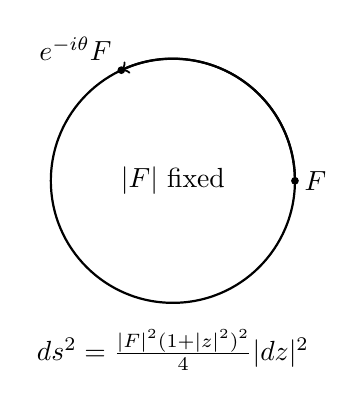
\begin{tikzpicture}[scale=1.0]
  \draw[thick] (0,0) circle (1.55);
  \draw[->,thick] (1.55,0) arc[start angle=0,end angle=115,radius=1.55];
  \fill (1.55,0) circle (1.4pt) node[right] {$F$};
  \fill (-0.655,1.405) circle (1.4pt) node[above left] {$e^{-i\theta}F$};
  \node at (0,0) {$|F|$ fixed};
  \node at (0,-2.15) {$ds^2=\frac{|F|^2(1+|z|^2)^2}{4}|dz|^2$};
\end{tikzpicture}
\caption{The associated family rotates the phase of the normalized Weierstrass function, $F\mapsto e^{-i\theta}F$. Since the metric depends on $|F|$ only, every member of the family has the same induced metric.}
\label{fig:cp-iv-0084-associated-family-phase}
\end{figure}


\begin{solution}
For Weierstrass data \((f,g)\), set
\[
\Phi_{(f,g)}
=
\left(
\frac12 f(1-g^2),
\frac{i}{2}f(1+g^2),
fg
\right),
\qquad
X(z)=\Re\int^z\Phi_{(f,g)}(\zeta)\,d\zeta.
\]
A direct computation gives
\[
\Phi_{(f,g)}\cdot\Phi_{(f,g)}=0,
\]
so the immersion is conformal, while holomorphicity of \(\Phi\) makes each coordinate of \(X\) harmonic; hence \(X\) is minimal.

The induced metric is
\[
ds^2
=
\frac{|f|^2(1+|g|^2)^2}{4}|dz|^2.
\]
Replace \(f\) by
\[
f_\theta=e^{-i\theta}f.
\]
Then \(|f_\theta|=|f|\), so
\[
ds_\theta^2=ds^2.
\]
Thus the family
\[
X_\theta
=
\Re\int^z\Phi_{(e^{-i\theta}f,g)}\,d\zeta
\]
consists of conformal minimal immersions that are locally isometric. This is the associated family.

Under a biholomorphic change of parameter \(z=\alpha(w)\), the data transform as
\[
\widetilde g(w)=g(\alpha(w)),
\qquad
\widetilde f(w)=f(\alpha(w))\alpha'(w).
\]
At a regular point of the Gauss map, \(g'(z_0)\neq0\), choosing \(\alpha=g^{-1}\) gives the normalized form
\[
(\widetilde f,\widetilde g)=(F,\operatorname{id}).
\]
The associated family is then simply \((e^{-i\theta}F,\operatorname{id})\).

For Enneper data \(f=1,\ g=z\), this yields \(f_\theta=e^{-i\theta}\), so all members of the Enneper associated family have the same first fundamental form.
\end{solution}


\begin{problem}[CP-IV-0089]
\label{prob:cp-iv-0089}
\par\noindent\textbullet\quad The data $(f,g)$ are two complex functions, hence define a map $(f,g):D\to\mathbb C^2$,
	but $(f,g)$ is \emph{not} the surface. It is the holomorphic data used to build $\Phi$ and then $\phi$.

\medskip
\textbf{One-sentence summary.}
The surface is $\phi:D\subset\mathbb C\to\mathbb R^3$; the complex derivative produces $\Phi=2\phi_z\in\mathbb C^3$ with
$\Phi\cdot\Phi=0$; and the functions $f=\Phi_1-i\Phi_2$ and $g=\Phi_3/f$ encode $\Phi$, with $g$ representing the Gauss map
(stereographic coordinate) and $f\,dz$ controlling the conformal scale.

\medskip

A parametrized surface patch is a smooth map
\[
\phi : D \subset \mathbb R^2 \to \mathbb R^3,\qquad (x,y)\mapsto \phi(x,y).
\]
Hence it has the usual partial derivatives with respect to the two real parameters:
\[
\phi_x(x,y)=\frac{\partial \phi}{\partial x}(x,y),\qquad
\phi_y(x,y)=\frac{\partial \phi}{\partial y}(x,y).
\]
Writing $\phi=(\phi^1,\phi^2,\phi^3)$, these are
\[
\phi_x=\big(\partial_x\phi^1,\partial_x\phi^2,\partial_x\phi^3\big)\in\mathbb R^3,
\qquad
\phi_y=\big(\partial_y\phi^1,\partial_y\phi^2,\partial_y\phi^3\big)\in\mathbb R^3.
\]
If we identify $(x,y)$ with the complex coordinate $z=x+iy$, we often write $\phi(z)$ instead of $\phi(x,y)$; this is only
a change of notation.
The complex derivatives are defined by the linear combinations
\[
\phi_z=\tfrac12(\phi_x-i\phi_y),\qquad
\phi_{\bar z}=\tfrac12(\phi_x+i\phi_y),
\]
which package the two real tangent vectors $\phi_x,\phi_y$ into complex form.

\medskip

A surface is \emph{minimal} if and only if its mean curvature satisfies $H\equiv 0$.
For an immersion $\phi:D\subset\mathbb R^2\to\mathbb R^3$ there is the fundamental identity
\[
\Delta_g \phi = 2H\,N,
\]
where $\Delta_g$ is the Laplace--Beltrami operator of the induced metric $g$ and $N$ is the unit normal.
Thus $H=0$ is equivalent to $\Delta_g\phi=0$.

If $(x,y)$ are \emph{conformal} (isothermal) coordinates, then
\[
g=\lambda^2(dx^2+dy^2)\qquad (E=G=\lambda^2,\;F=0),
\]
and the Laplace--Beltrami operator simplifies to
\[
\Delta_g = \frac{1}{\lambda^2}\Delta,
\qquad
\Delta=\partial_x^2+\partial_y^2.
\]
Substituting into $\Delta_g\phi=2H N$ yields
\[
\frac{1}{\lambda^2}\Delta\phi = 2H N
\quad\Longrightarrow\quad
\Delta\phi = 2\lambda^2 H N.
\]
Hence, for a minimal surface ($H=0$), we obtain $\Delta\phi=0$.

Finally, since $\Delta = 4\,\partial_z\partial_{\bar z}$, the equation $\Delta\phi=0$ implies
\[
\partial_{\bar z}\phi_z=\partial_{\bar z}(\partial_z\phi)=0,
\]
so $\phi_z$ is holomorphic as a $\mathbb C^3$-valued function.

\medskip

Write the immersion as
\[
\phi(x,y)=(\phi^1(x,y),\phi^2(x,y),\phi^3(x,y))\in\mathbb R^3.
\]
Then
\[
\phi_x=(\partial_x\phi^1,\partial_x\phi^2,\partial_x\phi^3)\in\mathbb R^3,
\qquad
\phi_y=(\partial_y\phi^1,\partial_y\phi^2,\partial_y\phi^3)\in\mathbb R^3.
\]
By definition,
\[
\phi_z=\tfrac12(\phi_x-i\phi_y),
\]
so each component is a complex number:
\[
\phi_z=
\left(
\tfrac12(\partial_x\phi^1-i\partial_y\phi^1),\
\tfrac12(\partial_x\phi^2-i\partial_y\phi^2),\
\tfrac12(\partial_x\phi^3-i\partial_y\phi^3)
\right)\in\mathbb C^3.
\]
Thus $\phi$ takes values in $\mathbb R^3$, but its complex derivative $\phi_z$ is a complex linear combination of real
tangent vectors and naturally lives in the complexified space $\mathbb C^3$.

Moreover, saying that $\phi_z$ is \emph{holomorphic as a $\mathbb C^3$-valued function} means
\[
\partial_{\bar z}\phi_z=0,
\]
equivalently $\partial_{\bar z}(\phi_z^k)=0$ for each component $k=1,2,3$.

\medskip

Although $\phi:D\to\mathbb R^3$ is real-valued, its complex derivative
\[
\phi_z=\tfrac12(\phi_x-i\phi_y)
\]
is $\mathbb C^3$-valued. Set
\[
\Phi:=2\phi_z \in \mathbb C^3.
\]
Since $\Phi$ is holomorphic, we can integrate componentwise to obtain a holomorphic map
\[
\Psi(z)=\int^z \Phi(\zeta)\,d\zeta \in \mathbb C^3
\]
(well-defined on simply connected domains, up to an additive constant). The original immersion is then recovered by taking
the real part componentwise:
\[
\phi(z)=\Re \Psi(z)=\Re\int^z \Phi(\zeta)\,d\zeta \in \mathbb R^3.
\]
Thus we \emph{temporarily} work in the complexified space $\mathbb C^3$ to exploit holomorphicity, and then take $\Re$ to
return to a surface in $\mathbb R^3$.

	\medskip
	\textbf{Why $g$ is the Gauss map, but $f$ is not.}

	Let $X=\phi_{(f,g)}:D\subset\mathbb C\to\mathbb R^3$ be a conformal minimal immersion given by the Weierstrass data $(f,g)$:
	\[
	X(z)=\Re\int^z \Phi_{(f,g)}(\zeta)\,d\zeta,
	\qquad
	\Phi_{(f,g)}(z)
	=
	\Bigl(\tfrac12 f(1-g^2),\ \tfrac{i}{2}f(1+g^2),\ fg\Bigr).
	\]
	The induced metric is
	\[
	ds^2=\frac{|f|^2(1+|g|^2)^2}{4}\,|dz|^2.
	\]

	\smallskip
	\textbf{1) The Gauss map and the role of $g$.}
	The \emph{Gauss map} of $X$ is the unit normal field
	\[
	N:D\to \mathbb S^2.
	\]
	Let $\sigma:\mathbb S^2\setminus\{(0,0,1)\}\to\mathbb C$ be stereographic projection. A fundamental fact of the Weierstrass
	representation is that
	\[
	g=\sigma\circ N,
	\]
	so $g$ is (locally) the complex coordinate of the normal direction. Equivalently, $N$ can be recovered from $g$ by inverse
	stereographic projection:
	\[
	N
	=
	\frac{1}{1+|g|^2}\,\bigl(2\Re g,\ 2\Im g,\ |g|^2-1\bigr).
	\]
	Thus \emph{$g$ encodes the direction of the unit normal}, i.e.\ the Gauss map.

	\smallskip
	\textbf{2) The role of $f$ (conformal scale, not normals).}
	The function $f$ is \emph{not} a Gauss map. It controls the conformal scale of the parametrization via the metric:
	\[
	ds^2=\frac{|f|^2(1+|g|^2)^2}{4}\,|dz|^2.
	\]
	In particular, $|f|$ determines local lengths in the parameter domain (together with $|g|$), while the argument of $f$ is a
	constant ``phase'' in the holomorphic differential. There is no formula expressing $N$ purely in terms of $f$.

	\smallskip
	\textbf{3) Why it may look like ``both are Gauss maps'' after a reparametrization.}
	Non-uniqueness comes from biholomorphic reparametrization. If $\alpha:W\to D$ is biholomorphic, then
	$X\circ\alpha$ is again a Weierstrass immersion with new data
	\[
	\tilde g(w)=g(\alpha(w)),
	\qquad
	\tilde f(w)=f(\alpha(w))\,\alpha'(w).
	\]
	If $g'(z_0)\neq 0$, then $g$ has a local holomorphic inverse $g^{-1}$ near $z_0$. Choosing $\alpha=g^{-1}$ gives
	\[
	\tilde g(w)=g(g^{-1}(w))=w=\mathrm{id}(w),
	\qquad
	\tilde f(w)=f(g^{-1}(w))\,(g^{-1})'(w)=:F(w).
	\]
	So locally we may normalize the data to $(F,\mathrm{id})$. This does \emph{not} mean that $F$ is a Gauss map; it only means we
	chose coordinates so that the Gauss-map coordinate becomes the parameter $w$ itself.

	\smallskip
	\textbf{Summary.}
	\[
	\boxed{\text{$g$ is (stereographic) Gauss map data, while $f\,dz$ controls the conformal scale of the immersion.}}
	\]

	\medskip
	\noindent
	\textbf{Idea (one picture).}
	The Weierstrass pair $(f,g)$ is not unique because we may reparametrize the domain by any biholomorphic map
	$\alpha:W\to D$ (change of complex coordinate). Under $z=\alpha(w)$, the same minimal immersion can be written again in
	Weierstrass form with new data
	\[
	\tilde g(w)=g(\alpha(w)),\qquad \tilde f(w)=f(\alpha(w))\,\alpha'(w).
	\]
	At a regular point $z_0$ of $g$ (where $g'(z_0)\neq 0$), the holomorphic inverse function theorem allows us to choose
	$\alpha=g^{-1}$ locally, which normalizes the Gauss-map coordinate to $\tilde g=\mathrm{id}$ and leaves only one holomorphic
	function $F:=\tilde f$. In this normalized form $(F,\mathrm{id})$, multiplying $F$ by a unimodular constant
	$e^{-i\theta}$ rotates the complex differential by a constant phase but does not change its modulus; hence the induced metric
	\[
	ds^2=\frac{|F|^2(1+|z|^2)^2}{4}\,|dz|^2
	\]
	is unchanged. Therefore the associated family $\{\phi_{e^{-i\theta}F}\}_{\theta\in\mathbb R}$ consists of locally isometric
	minimal surfaces.
	\medskip

	\medskip
	\noindent
	\textbf{Geometric meaning of $g$ (Gauss map in complex coordinates).}
	For a conformal minimal immersion $\phi:D\to\mathbb R^3$, let $N:D\to\mathbb S^2$ be the unit normal (Gauss map).
	Stereographic projection $\sigma:\mathbb S^2\setminus\{N_0\}\to\mathbb C$ (from the north pole $N_0=(0,0,1)$) identifies
	$\mathbb S^2$ (minus one point) with the complex plane. The Weierstrass function $g$ is precisely this normal direction
	written as a complex number:
	\[
	g=\sigma\circ N.
	\]
	Thus $g$ encodes how the surface bends (how the normal changes), while $f\,dz$ controls the conformal scale; the induced
	metric is
	\[
	ds^2=\frac{|f|^2(1+|g|^2)^2}{4}\,|dz|^2,
	\]
	so the modulus $|f|$ matters for lengths, whereas a constant phase factor $e^{-i\theta}$ does not change $ds^2$.
	\medskip

	\medskip
	\noindent
	\textbf{Bidirectional view: $g$ encodes the unit normal.}
	Stereographic projection $\sigma:\mathbb S^2\setminus\{N_0\}\to\mathbb C$ identifies (almost all of) the unit sphere with
	the complex plane. For a conformal immersion $\phi$, the Gauss map $N:D\to\mathbb S^2$ gives the unit normal, and
	\[
	g=\sigma\circ N
	\]
	is exactly that normal direction written as a complex number. Conversely, $g$ determines the unit normal by inverse
	stereographic projection:
	\[
	N=\sigma^{-1}(g)=\frac{1}{1+|g|^2}\bigl(2\Re g,\ 2\Im g,\ |g|^2-1\bigr)\in\mathbb S^2.
	\]
	\medskip

	\clearpage
\end{problem}

\begin{solution}
Let
\[
X:D\longrightarrow\mathbb R^3
\]
be a conformal minimal immersion. In complex coordinates \(z=x+iy\),
\[
X_z=\frac12(X_x-iX_y)\in\mathbb C^3.
\]
Minimality in conformal coordinates implies
\[
\partial_{\bar z}X_z=0,
\]
so
\[
\Phi:=2X_z
\]
is holomorphic. Conformality gives the isotropy condition
\[
\Phi\cdot\Phi=0.
\]

On the set where \(\Phi_1-i\Phi_2\neq0\), define
\[
f=\Phi_1-i\Phi_2,
\qquad
g=\frac{\Phi_3}{f}.
\]
Using \(\Phi_1^2+\Phi_2^2+\Phi_3^2=0\), one obtains
\[
\Phi
=
\left(
\frac12f(1-g^2),
\frac{i}{2}f(1+g^2),
fg
\right).
\]
Hence
\[
X(z)=\Re\int^z\Phi(\zeta)\,d\zeta.
\]

The two pieces of data have different geometric meanings. The function \(g\) is the stereographic coordinate of the Gauss map:
\[
N
=
\frac{1}{1+|g|^2}
\bigl(2\Re g,\,2\Im g,\,|g|^2-1\bigr).
\]
Thus \(g\) determines the normal direction. By contrast, \(f\,dz\) controls the conformal scale, since
\[
ds^2
=
\frac{|f|^2(1+|g|^2)^2}{4}|dz|^2.
\]
Therefore \((f,g)\) are not themselves the surface: they are holomorphic data from which the surface is reconstructed. Under a biholomorphic reparametrization \(z=\alpha(w)\),
\[
\widetilde g=g\circ\alpha,
\qquad
\widetilde f=(f\circ\alpha)\alpha',
\]
which explains the nonuniqueness of the data.
\end{solution}


\begin{problem}[CP-IV-0090]
\label{prob:cp-iv-0090}
(exact)

Let $f:U\to\mathbb{C}$ be holomorphic on a domain $U$.

	\par\noindent (a)\quad Show that, if $\overline{B}(a,r)\subset U$, then
	\[
	f(a)=\frac{1}{2\pi}\int_{0}^{2\pi} f(a+re^{it})\,dt.
	\]
	\par\noindent (b)\quad Suppose $a\in U$ is such that $|f(a)|=\max_{U}|f|$. Show that $|f|$ must be constant near $a$.
	\par\noindent (c)\quad Deduce that $f$ is constant on all of $U$.
	\quad\emph{Hint:} Consider $S=\{z\in U: |f(z)|=|f(a)|\}$.

If $\overline{B}(a,r)\subset U$, then
\[
f(a)=\frac{1}{2\pi i}\int_{|\zeta-a|=r}\frac{f(\zeta)}{\zeta-a}\,d\zeta.
\]
With $\zeta=a+re^{it}$ and $d\zeta=ire^{it}dt$, this becomes the circular average.

For an integrable complex function $g$, $\left|\int g\right|\le\int|g|$ with equality iff $g$ has a constant argument almost everywhere on the path of integration.

If $f$ is holomorphic on $\overline{B}(a,r)$, then for $n\ge1$,
\[
f^{(n)}(a)=\frac{n!}{2\pi i}\int_{|\zeta-a|=r}\frac{f(\zeta)}{(\zeta-a)^{n+1}}\,d\zeta.
\]
\end{problem}

\begin{solution}
\par\medskip\noindent\textbf{(a) Mean value property.}\quad 
By Cauchy’s formula,
\[
f(a)=\frac{1}{2\pi i}\int_{|\zeta-a|=r}\frac{f(\zeta)}{\zeta-a}\,d\zeta
=\frac{1}{2\pi i}\int_{0}^{2\pi}\frac{f(a+re^{it})}{re^{it}}\,(ire^{it})\,dt
=\frac{1}{2\pi}\int_{0}^{2\pi} f(a+re^{it})\,dt.
\]

\par\medskip\noindent\textbf{(b) Local constancy at an interior maximum.}\quad 
Assume $|f(a)|=\max_{U}|f|$. For $r>0$ with $\overline{B}(a,r)\subset U$,
\[
|f(a)|
=\left|\frac{1}{2\pi}\int_{0}^{2\pi} f(a+re^{it})\,dt\right|
\le \frac{1}{2\pi}\int_{0}^{2\pi}|f(a+re^{it})|\,dt
\le \frac{1}{2\pi}\int_{0}^{2\pi}|f(a)|\,dt
=|f(a)|.
\]
Thus equality holds throughout. Hence $|f(a+re^{it})|=|f(a)|$ and $f(a+re^{it})$ has a constant argument (the same as $f(a)$) for almost every $t$. Therefore
\[
f(a+re^{it})=f(a)\quad\text{for all }t,
\]
i.e. $f$ is constant on the circle $|z-a|=r$. For such an $r$, Cauchy’s formula for $n\ge1$ gives
\[
f^{(n)}(a)=\frac{n!}{2\pi i}\int_{|\zeta-a|=r}\frac{f(\zeta)}{(\zeta-a)^{n+1}}\,d\zeta
=\frac{n!}{2\pi i}\,f(a)\int_{|\zeta-a|=r}\frac{1}{(\zeta-a)^{n+1}}\,d\zeta=0.
\]
Hence the Taylor series of $f$ at $a$ is the constant $f(a)$; there exists $\rho>0$ such that $f\equiv f(a)$ on $B(a,\rho)$. In particular, $|f|$ is constant near $a$.

\par\medskip\noindent\textbf{(c) Constancy on the whole domain.}\quad 
Let $M=|f(a)|$ and $S=\{z\in U: |f(z)|=M\}$. The set $S$ is closed (preimage of $\{M\}$ under the continuous map $z\mapsto|f(z)|$). By part (b), for each $z\in S$ there exists a neighborhood on which $f$ is constant, hence that neighborhood lies in $S$; thus $S$ is open. Since $U$ is connected and $S\neq\varnothing$, we conclude $S=U$, so $|f|$ is constant on $U$, and by (b) (applied at any point) $f$ is constant on $U$.
\end{solution}

\begin{problem}[CP-IV-0092]
\label{prob:cp-iv-0092}
(restated).

Let $D\subset\mathbb C$ be simply connected and $0\notin D$.
Show that there exists a holomorphic function $F$ on $D$ with $F'(z)=1/z$ and $e^{F(z)}=z$ for $z\in D$
(i.e.\ $F$ is a branch of the logarithm on $D$).

\medskip
\end{problem}

\begin{solution}
\par\medskip\noindent\textbf{Solution to Problem 10.}\quad 
Fix $z_0\in D$ and define
\[
F(z)=\int_{z_0}^{z}\frac{d\zeta}{\zeta}.
\]
Since $1/\zeta$ is holomorphic on $D$ and $D$ is simply connected, the integral is path-independent; $F$ is holomorphic with $F'(z)=1/z$.
Let $G(z)=e^{F(z)}/z$. Then $G'(z)=0$, so $G$ is constant. Choosing $F(z_0)$ so that $G\equiv 1$ yields $e^{F(z)}=z$ on $D$.

\bigskip
\end{solution}

\begin{problem}[CP-IV-0096]
\label{prob:cp-iv-0096}
\par\noindent\textbullet\quad Suppose $f(1/n)=1/(n+1)$ for all $n$. Then
	\[
	h(z):=f(z)-\frac{z}{z+1}
	\]
	is holomorphic on $D(0,2)\setminus\{-1\}$, vanishes at $z=1/n$ for all $n$, and the set $\{1/n\}$ accumulates at $0$ in that domain.
	By the identity theorem, $h\equiv 0$ there, i.e.\ $f(z)=\dfrac{z}{z+1}$ on $D(0,2)\setminus\{-1\}$.
	But $\dfrac{z}{z+1}$ has a pole at $z=-1$, whereas $f$ is holomorphic there — a contradiction.
	Hence some $n$ satisfies $f(1/n)\ne 1/(n+1)$.

\bigskip
\end{problem}

\begin{solution}
Assume, for contradiction, that
\[
f(1/n)=\frac{1}{n+1}
\]
for every \(n\ge1\). Define
\[
h(z)=f(z)-\frac{z}{z+1}.
\]
On
\[
D(0,2)\setminus\{-1\},
\]
the function \(h\) is holomorphic, and
\[
h(1/n)=0
\]
for all \(n\). The zeros \(1/n\) accumulate at \(0\), which lies in the domain. By the identity theorem,
\[
h\equiv0
\]
on \(D(0,2)\setminus\{-1\}\). Hence
\[
f(z)=\frac{z}{z+1}
\]
there.

But the right-hand side has a pole at \(z=-1\), whereas \(f\) is holomorphic on all of \(D(0,2)\). This contradiction shows that the assumed equalities cannot hold for every \(n\). Therefore for some \(n\),
\[
f(1/n)\neq\frac1{n+1}.
\]
\end{solution}


\begin{problem}[CP-IV-0097]
\label{prob:cp-iv-0097}
(Real shear).

Let $T$ have real matrix $\begin{psmallmatrix}1&1\\ 0&1\end{psmallmatrix}$.
By the formulas,
\[
A=\frac{1+1}{2}+i\,\frac{0-1}{2}=1-\tfrac{i}{2},\qquad
B=\frac{1-1}{2}+i\,\frac{0+1}{2}=\tfrac{i}{2}.
\]
The image of the unit circle is an ellipse tilted by the shear. Since $B\neq0$, $T$ is not holomorphic.
The Jacobian is $|A|^2-|B|^2=(1^2+(\tfrac12)^2)-(\tfrac12)^2=1>0$, so orientation is preserved.
\end{problem}

\begin{solution}
For the real shear
\[
T(x,y)=(x+y,y),
\]
the real matrix is
\[
\begin{pmatrix}1&1\\0&1\end{pmatrix}.
\]
Writing \(T(z)=Az+B\overline z\), the standard formulas give
\[
A=\frac{1+1}{2}+i\frac{0-1}{2}
=
1-\frac{i}{2},
\]
and
\[
B=\frac{1-1}{2}+i\frac{0+1}{2}
=
\frac{i}{2}.
\]
Since \(B\neq0\), the shear is not holomorphic.

Its Jacobian is
\[
|A|^2-|B|^2
=
\left(1+\frac14\right)-\frac14
=
1>0,
\]
so orientation is preserved. The image of the unit circle under a nonconformal invertible real-linear map is an ellipse; here it is the familiar sheared circle.
\end{solution}


\begin{problem}[CP-IV-0102]
\label{prob:cp-iv-0102}
automorphism of the upper half-plane

Consider the M\"obius transformation
	\[
	T(z) = \frac{z-1}{z+1}.
	\]
	We work on the upper half-plane
	\[
	H = \{ z : \Im z > 0 \}
	\]
	with boundary the extended real line
	\[
	L = \mathbb R \cup \{\infty\}.
	\]

	Writing $z=x+iy$ with $y>0$, a direct computation yields
	\[
	\Im T(z)
	= \Im\!\left(\frac{z-1}{z+1}\right)
	= \frac{\Im z}{|z+1|^2}
	= \frac{y}{|z+1|^2} > 0.
	\]
	Hence
	\[
	\Im z > 0 \quad\Longleftrightarrow\quad \Im T(z) > 0,
	\]
	so $T$ is a non-affine automorphism of the upper half-plane and maps
	$L$ to itself.

	Along the boundary $L$ we have:
	\[
	T(1) = \frac{1-1}{1+1} = 0, \qquad
	T(-1) = \frac{-1-1}{-1+1} = \infty, \qquad
	T(\infty) = \lim_{z\to\infty}\frac{z-1}{z+1} = 1.
	\]
	Thus, in the three-point normalization language we may choose
	\[
	a = 1, \quad b = -1, \quad c = \infty
	\quad\text{on } L_1 = L,
	\]
	and
	\[
	A = 0, \quad B = \infty, \quad C = 1
	\quad\text{on } L_2 = L.
	\]
	Then $T$ is exactly the M\"obius map sending
	\[
	a \mapsto A,\qquad b \mapsto B,\qquad c \mapsto C,
	\]
	i.e.
	\[
	1 \mapsto 0,\qquad -1 \mapsto \infty,\qquad \infty \mapsto 1.
	\]

	When one of the boundary points is $\infty$, the cross-ratio formula
	simplifies: for $(a,b,c)=(1,-1,\infty)$ we have
	\[
	\Phi(z) = \frac{(z-a)(c-b)}{(z-b)(c-a)}
	= \frac{(z-1)}{(z+1)},
	\]
	so in this case $T(z) = \Phi(z)$ is precisely the three-point
	normalization carrying $(1,-1,\infty)$ to $(0,\infty,1)$ on the same
	boundary line.

	Figures~\ref{fig:hp-auto-z} and \ref{fig:hp-auto-w} illustrate the
	action of $T$ on the upper half-plane.
\begin{figure}[ht]
  \centering
  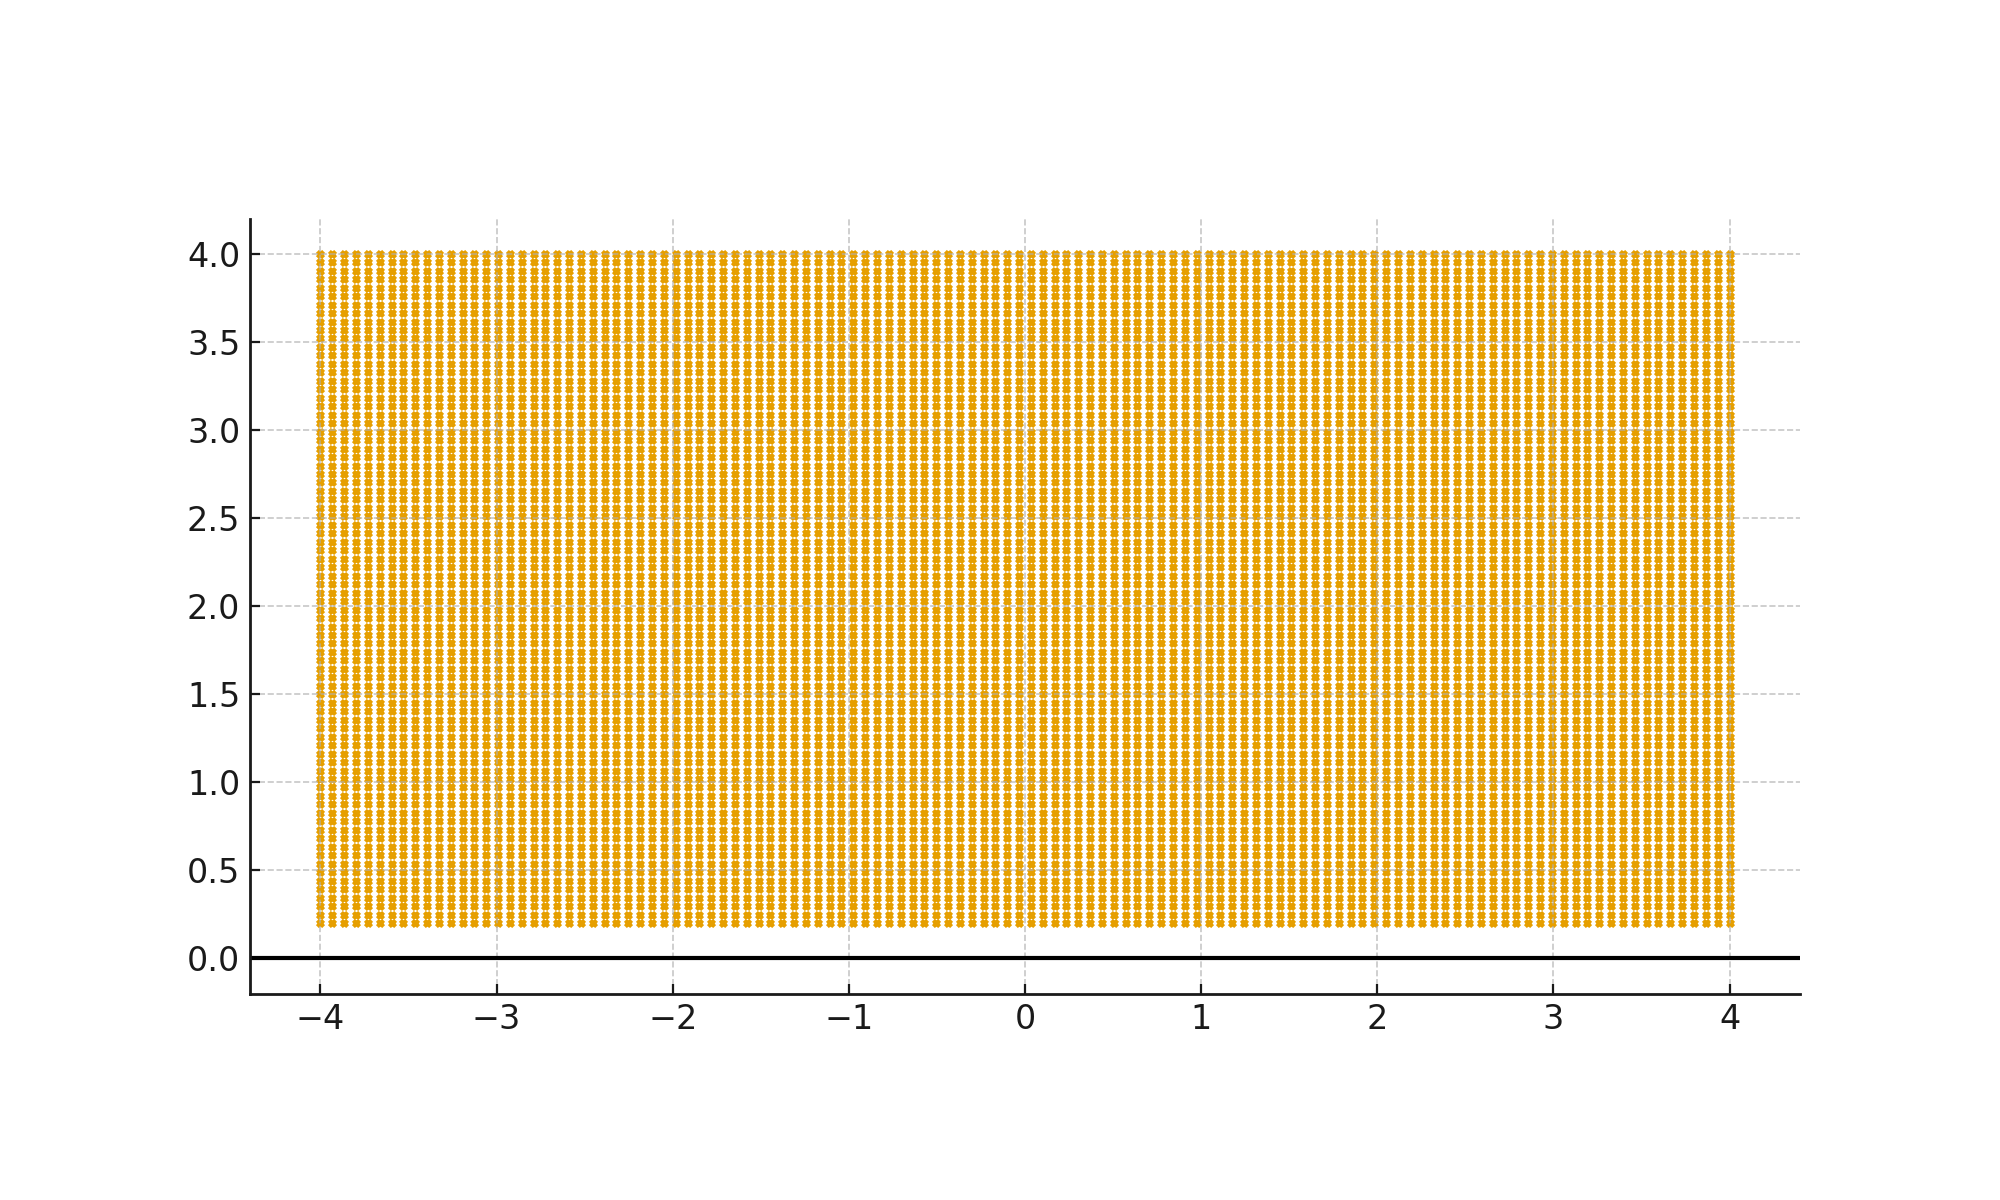
\includegraphics[width=0.78\textwidth]{figures/part04/cp_iv_0102_hp_auto_z_plane.png}
  \caption{Half-plane automorphism: source \(z\)-plane.}
  \label{fig:hp-auto-z}
\end{figure}

\begin{figure}[ht]
  \centering
  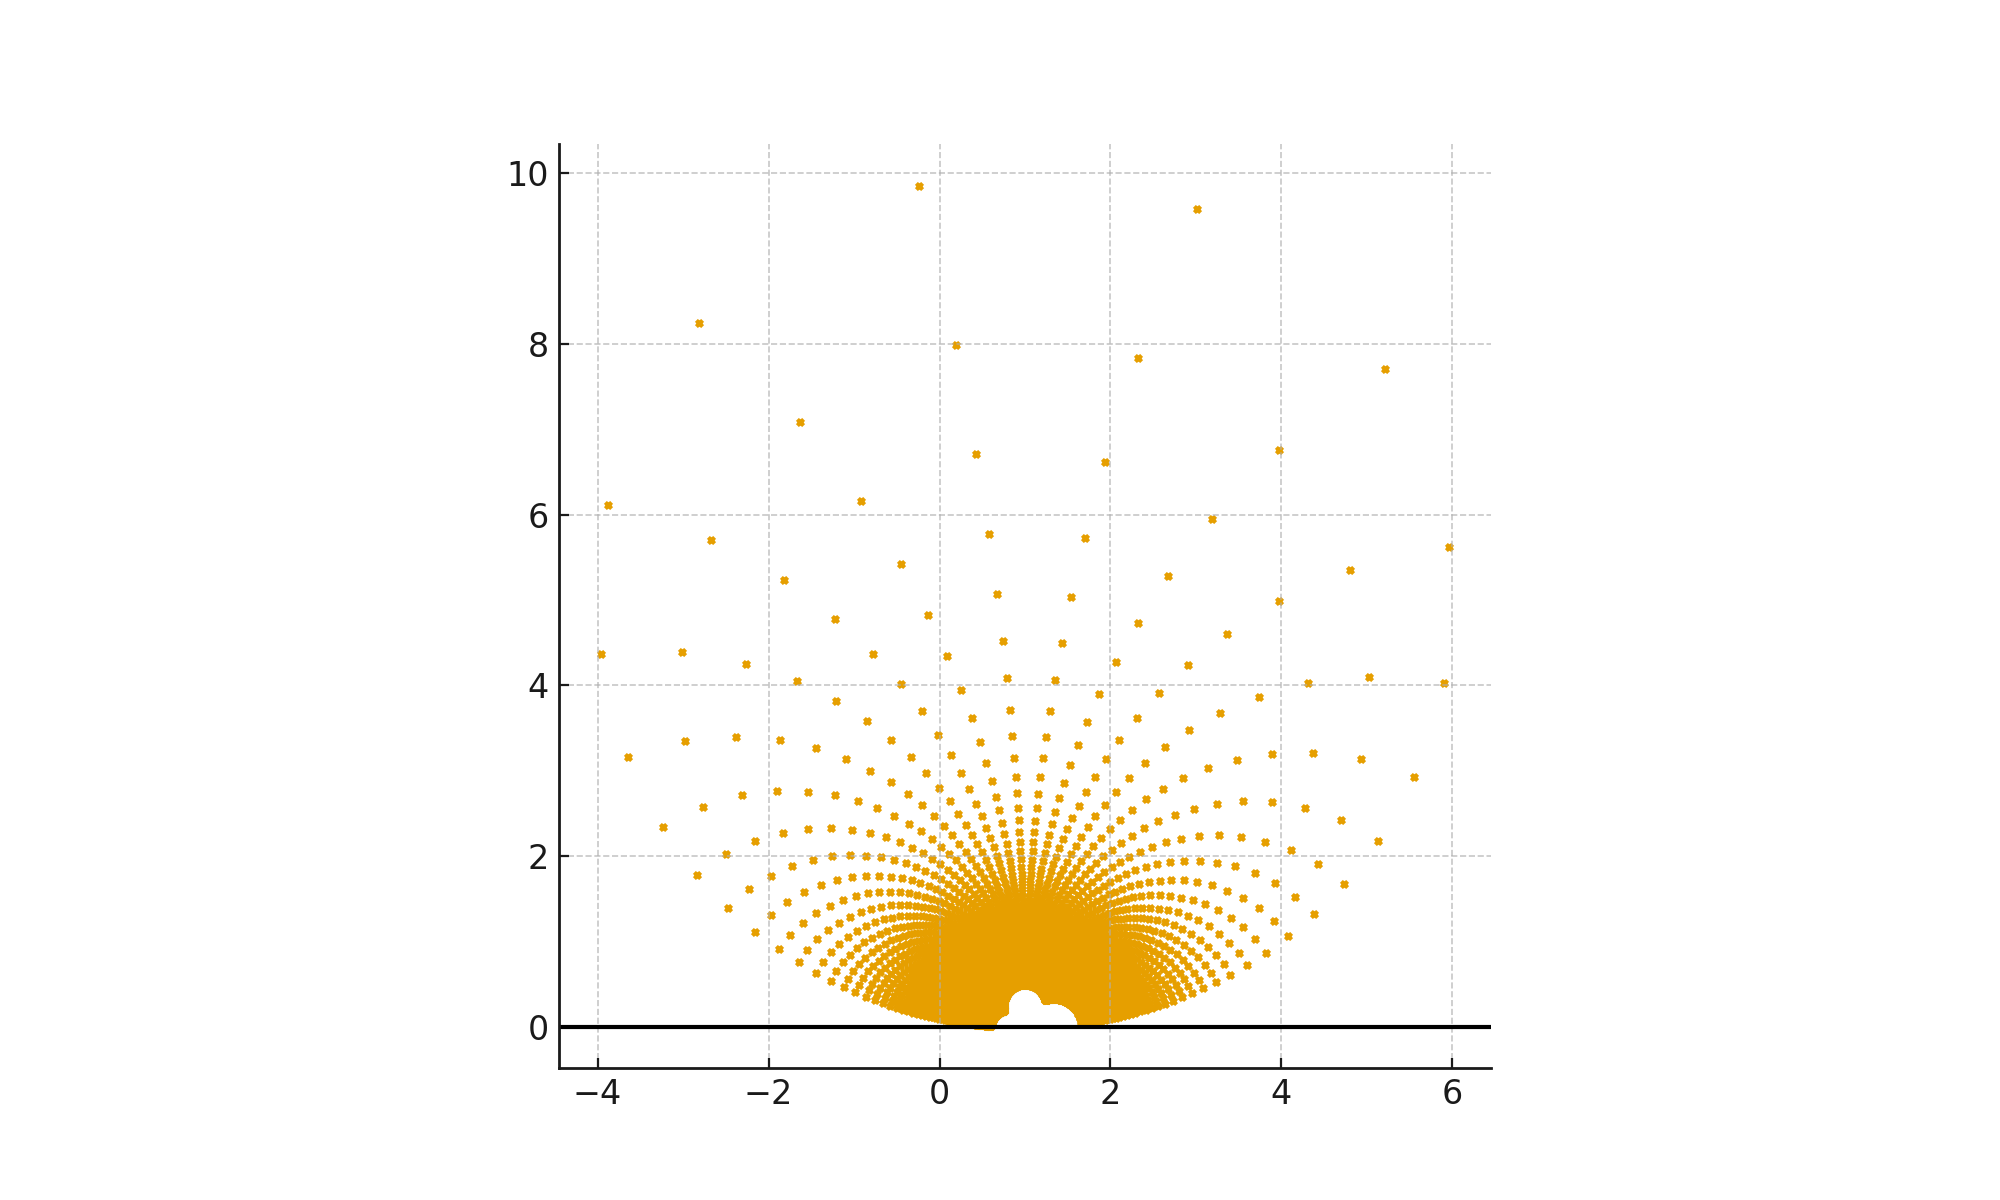
\includegraphics[width=0.78\textwidth]{figures/part04/cp_iv_0102_hp_auto_w_plane.png}
  \caption{Half-plane automorphism: image \(w\)-plane.}
  \label{fig:hp-auto-w}
\end{figure}


	Let
	\[
	H_1 = \{ z : \Im z > 0 \}, \qquad L_1 = \mathbb R,
	\]
	and
	\[
	H_2 = \{ w : \Re w > 1 \}, \qquad
	L_2 = \{ w : \Re w = 1 \}.
	\]

	Choose boundary triples
	\[
	a = -1,\quad b = 0,\quad c = 2 \in L_1,
	\]
	\[
	A = 1-i,\quad B = 1,\quad C = 1+i \in L_2,
	\]
	listed in the same cyclic order (bottom to top).

	The cross-ratio map sending $L_1$ to the real axis is
	\[
	\Phi(z)
	= \frac{(z-a)(c-b)}{(z-b)(c-a)}
	= \frac{2(z+1)}{3z},
	\]
	so that $\Phi(a)=0$, $\Phi(b)=\infty$, $\Phi(c)=1$.
	Similarly, the map sending $L_2$ to the real axis is
	\[
	\Psi(w)
	= \frac{(w-A)(C-B)}{(w-B)(C-A)}
	= \frac{w-1+i}{2(w-1)},
	\]
	for which $\Psi(A)=0$, $\Psi(B)=\infty$, $\Psi(C)=1$.

	The desired map $T : H_1 \to H_2$ is defined by
	\[
	\Psi(T(z)) = \Phi(z),
	\]
	i.e.\ $T(z) = \Psi^{-1}(\Phi(z))$. Solving $\Psi(w)=\xi$ for $w$ gives
	\[
	\Psi^{-1}(\xi) = \frac{2\xi - 1 + i}{2\xi - 1},
	\]
	and hence
	\[
	T(z)
	= \frac{2\Phi(z) - 1 + i}{2\Phi(z) - 1},
	\qquad
	\Phi(z) = \frac{2(z+1)}{3z}.
	\]
	Then
	\[
	T(-1) = 1-i,\qquad T(0) = 1,\qquad T(2) = 1+i,
	\]
	and $T$ maps the upper half-plane $\Im z>0$ biholomorphically onto the
	half-plane $\Re w>1$.

	Figures~\ref{fig:hp-h1h2-z} and \ref{fig:hp-h1h2-w}
	illustrate this non-automorphism half-plane map.
\end{problem}
\begin{figure}[ht]
  \centering
  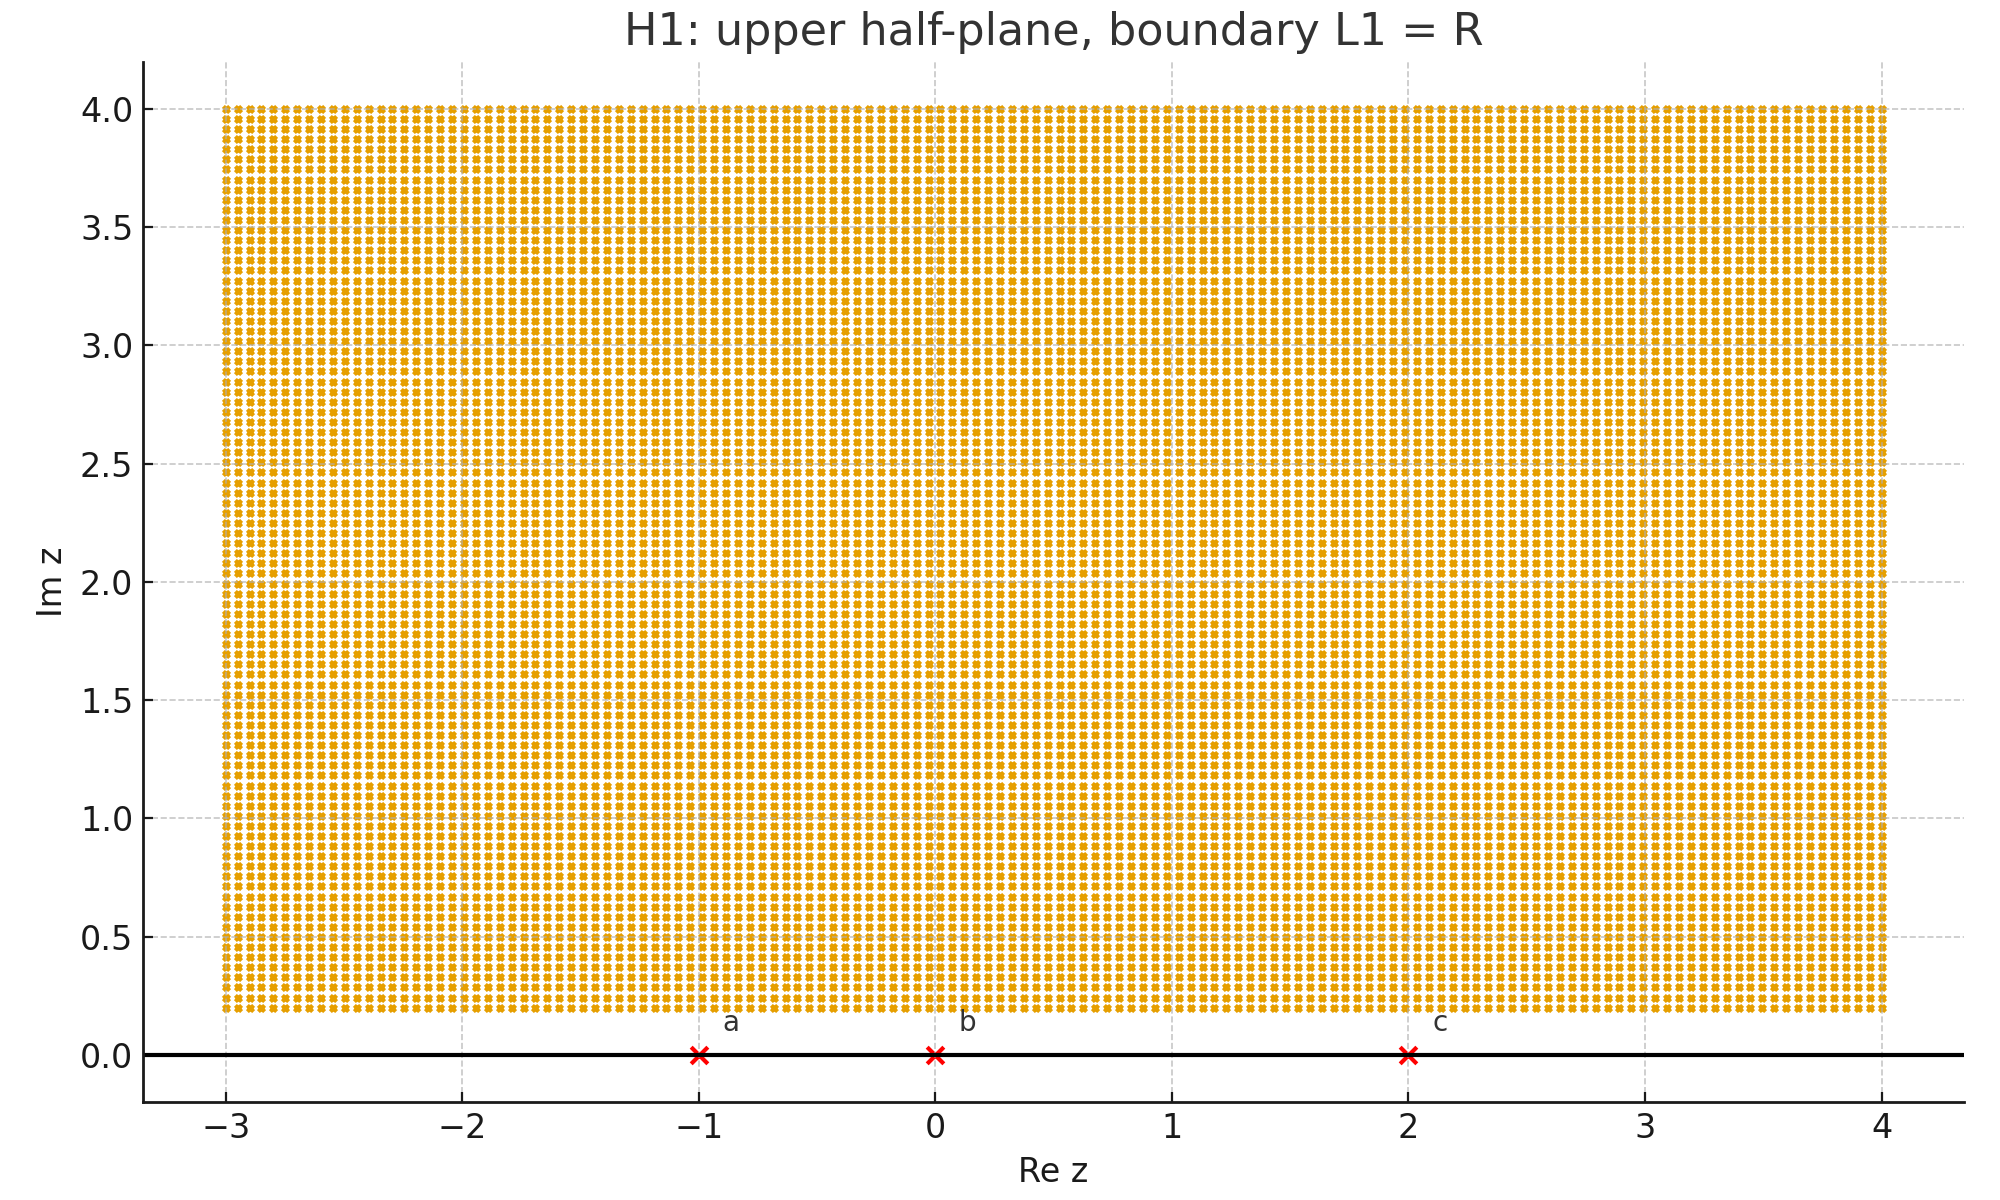
\includegraphics[width=0.78\textwidth]{figures/part04/cp_iv_0102_hp_h1h2_z_plane.png}
  \caption{Half-plane-to-half-plane map: source \(z\)-plane.}
  \label{fig:hp-h1h2-z}
\end{figure}

\begin{figure}[ht]
  \centering
  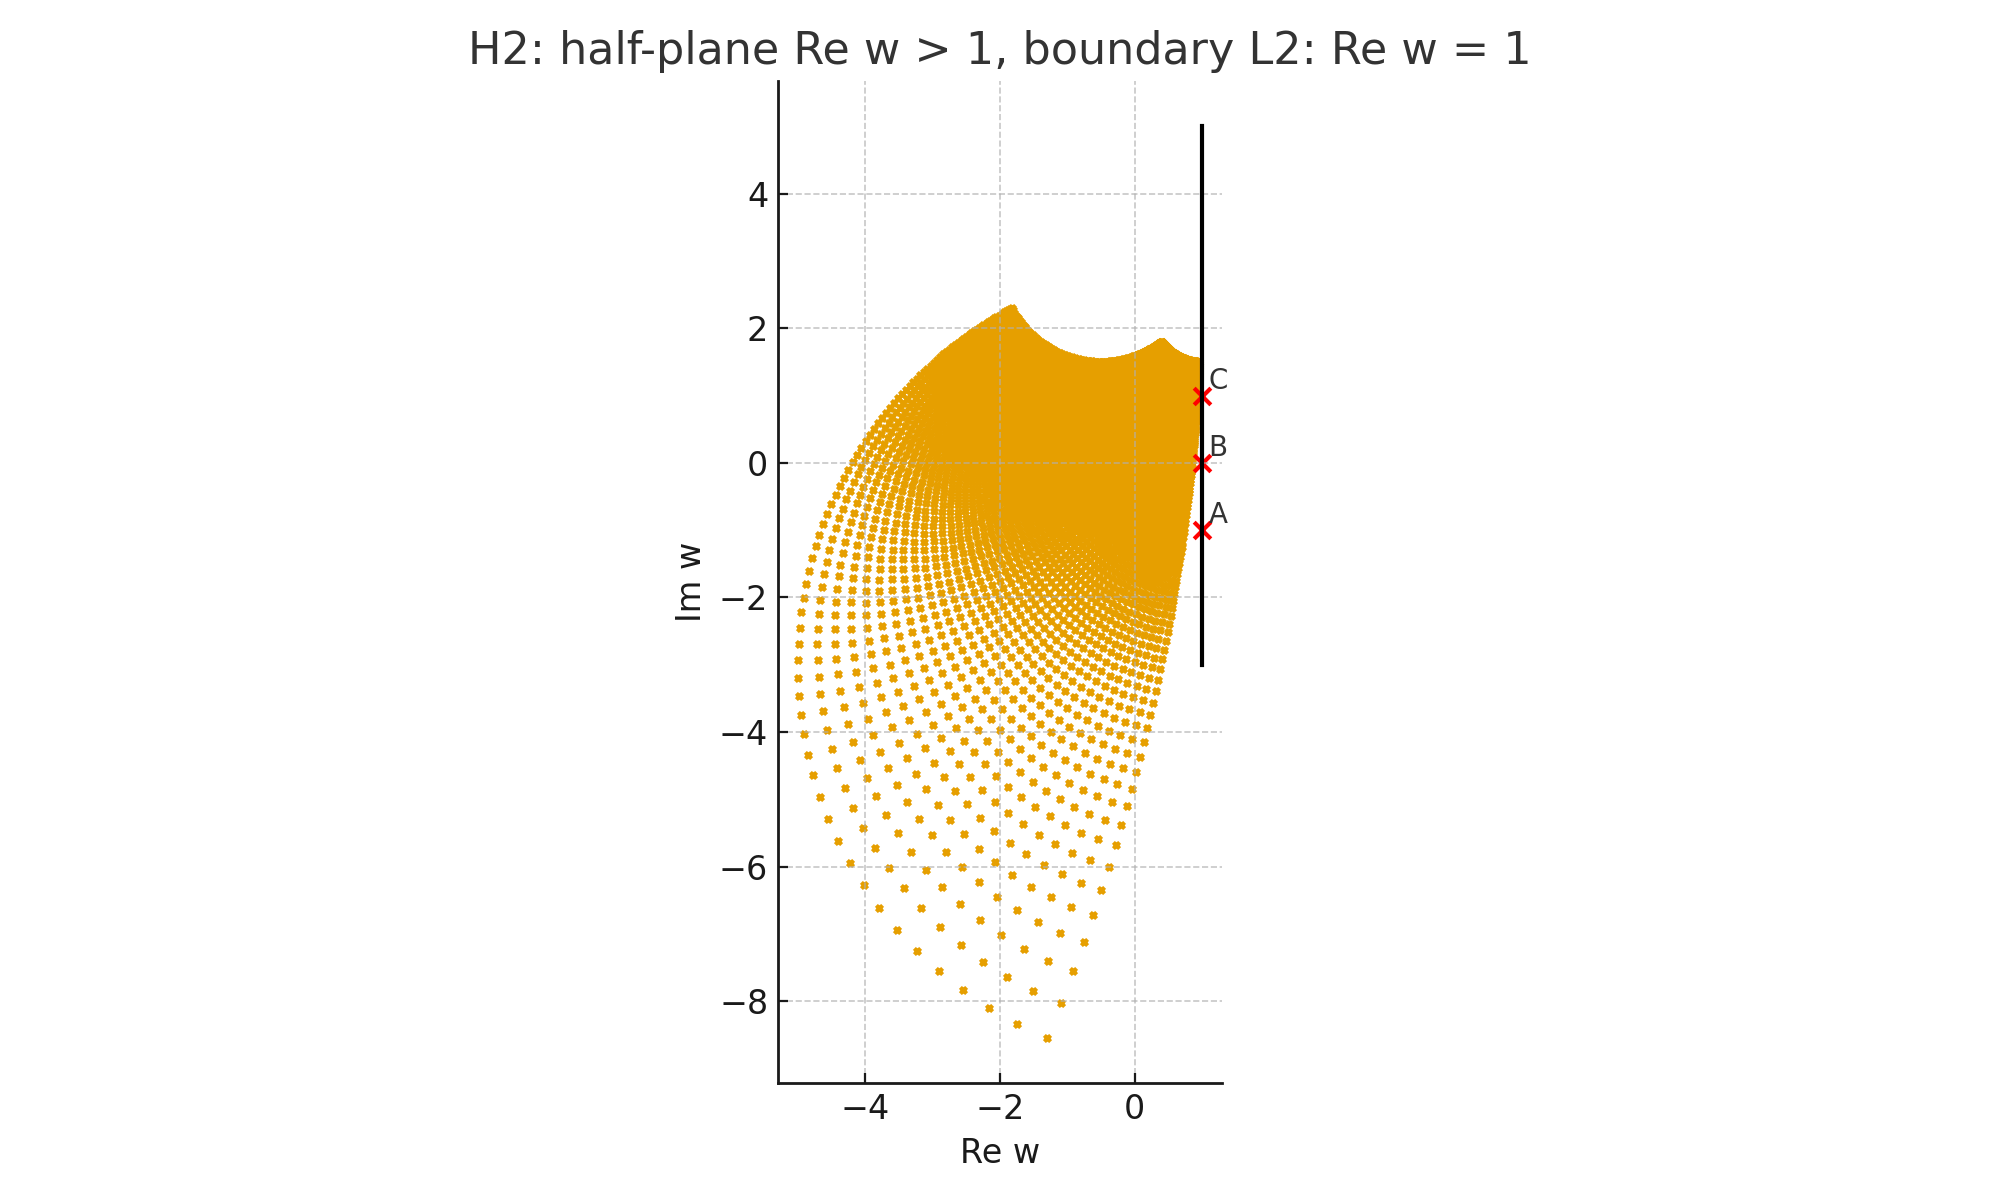
\includegraphics[width=0.78\textwidth]{figures/part04/cp_iv_0102_hp_h1h2_w_plane.png}
  \caption{Half-plane-to-half-plane map: image \(w\)-plane.}
  \label{fig:hp-h1h2-w}
\end{figure}

\begin{solution}
First consider
\[
T(z)=\frac{z-1}{z+1}.
\]
For \(z=x+iy\) with \(y>0\),
\[
\Im T(z)
=
\frac{2y}{|z+1|^2}>0.
\]
Hence \(T\) maps the upper half-plane to itself. Since
\[
T(1)=0,\qquad
T(-1)=\infty,\qquad
T(\infty)=1,
\]
it is precisely the M\"obius normalization taking
\[
(1,-1,\infty)\longmapsto(0,\infty,1).
\]
Its inverse is again M\"obius, so \(T\) is an automorphism of the upper half-plane.

For the second normalization, let
\[
a=-1,\quad b=0,\quad c=2,
\qquad
A=1-i,\quad B=1,\quad C=1+i.
\]
The source and target cross-ratio coordinates are
\[
\Phi(z)=\frac{2(z+1)}{3z},
\qquad
\Psi(w)=\frac{w-1+i}{2(w-1)}.
\]
Solving \(\Psi(w)=\xi\) gives
\[
\Psi^{-1}(\xi)
=
\frac{2\xi-1+i}{2\xi-1}.
\]
Therefore
\[
T(z)=\Psi^{-1}(\Phi(z)).
\]
Substitution gives
\[
T(-1)=1-i,\qquad
T(0)=1,\qquad
T(2)=1+i.
\]
Since the boundary triples occur in corresponding order, the chosen upper half-plane is carried biholomorphically to the half-plane \(\Re w>1\).
\end{solution}



\begin{problem}[CP-IV-0106]
\label{prob:cp-iv-0106}
(restated)

Let $\Gamma$ be a simple smooth positively oriented closed curve in the plane, and let $f$ be continuously differentiable on $\Gamma$.
Define, for $z\in\mathbb{C}\setminus\Gamma$,
\[
F(z):=\frac{1}{2\pi i}\int_{\Gamma}\frac{f(\zeta)}{\zeta-z}\,d\zeta .
\]
This integral diverges when $z$ approaches a point $\zeta_0\in\Gamma$ with $f(\zeta_0)\neq 0$.
Define the principal value at $\zeta_0$ by
\[
\operatorname{P.V.}\,\frac{1}{2\pi i}\int_{\Gamma}\frac{f(\zeta)}{\zeta-\zeta_0}\,d\zeta
\;:=\;
\lim_{\varepsilon\to 0^+}\frac{1}{2\pi i}
\int_{\Gamma_\varepsilon}\frac{f(\zeta)}{\zeta-\zeta_0}\,d\zeta,
\]
where $\Gamma_\varepsilon$ is $\Gamma$ with a small open arc of radius $\varepsilon$ around $\zeta_0$ removed (the remaining part is traversed with the original orientation).

\bigskip\hrule\bigskip

For $z\notin\Gamma$ the integrand is continuous on $\Gamma$ and the function $F$ is well defined and holomorphic in each of the two components of $\mathbb{C}\setminus\Gamma$ (the interior and the exterior).
Differentiation under the integral sign gives
\[
F'(z)=\frac{1}{2\pi i}\int_{\Gamma}\frac{f(\zeta)}{(\zeta-z)^2}\,d\zeta,
\qquad z\in\mathbb{C}\setminus\Gamma.
\]

If $f$ extends to a function holomorphic in the interior of $\Gamma$ and continuous on $\overline{\mathrm{int}(\Gamma)}$, then the Cauchy integral formula yields
\[
F(z)=f(z)\quad\text{for }z\text{ in the interior of }\Gamma,
\qquad
F(z)=0\quad\text{for }z\text{ in the exterior and }|z|\ \text{large}.
\]

At $z=\zeta_0\in\Gamma$ the kernel $(\zeta-\zeta_0)^{-1}$ has a simple pole on the contour.
The principal value extracts the finite, symmetric part of the singular integral by removing a small arc around the pole and letting its size shrink to $0$.

\bigskip\hrule\bigskip

Let $F^\pm(\zeta_0)$ denote the limits of $F(z)$ as $z\to\zeta_0\in\Gamma$
from the interior $(+)$ and from the exterior $(-)$ along nontangential approaches.
If $f\in C^1(\Gamma)$, then these limits exist and
\[
\boxed{
\begin{aligned}
F^{+}(\zeta_0) &= \frac{1}{2}\,f(\zeta_0)
\;+\;\operatorname{P.V.}\,\frac{1}{2\pi i}\int_{\Gamma}\frac{f(\zeta)}{\zeta-\zeta_0}\,d\zeta,\\[6pt]
F^{-}(\zeta_0) &= -\frac{1}{2}\,f(\zeta_0)
\;+\;\operatorname{P.V.}\,\frac{1}{2\pi i}\int_{\Gamma}\frac{f(\zeta)}{\zeta-\zeta_0}\,d\zeta.
\end{aligned}}
\]
Consequently,
\[
\boxed{\,F^{+}(\zeta_0)-F^{-}(\zeta_0)=f(\zeta_0)\,}
\qquad\text{and}\qquad
\boxed{\,\frac{F^{+}(\zeta_0)+F^{-}(\zeta_0)}{2}
=\operatorname{P.V.}\,\frac{1}{2\pi i}\int_{\Gamma}\frac{f(\zeta)}{\zeta-\zeta_0}\,d\zeta.}
\]

\bigskip

Fix $\zeta_0\in\Gamma$ and replace a small arc of $\Gamma$ near $\zeta_0$ by a circle of radius $\varepsilon$ centered at $\zeta_0$, lying inside (for $F^+$) or outside (for $F^-$) the domain. Then
\[
F(z)=\frac{1}{2\pi i}\!\!\int_{\Gamma_\varepsilon}\!\!\frac{f(\zeta)}{\zeta-z}\,d\zeta
\;+\;\frac{1}{2\pi i}\!\!\int_{C_\varepsilon}\!\!\frac{f(\zeta)}{\zeta-z}\,d\zeta,
\]
where $C_\varepsilon$ is the small circular arc. Let $z\to\zeta_0$ from the chosen side.
The first integral tends to the principal value term.
On $C_\varepsilon$, write $f(\zeta)=f(\zeta_0)+o(1)$ and compute
\[
\frac{1}{2\pi i}\int_{C_\varepsilon}\frac{f(\zeta_0)}{\zeta-\zeta_0}\,d\zeta
=\pm\frac{1}{2}f(\zeta_0),
\]
with the sign $+$ for the inner indentation and $-$ for the outer one (by orientation).
Adding the contributions yields the two Plemelj formulas above.

\bigskip\hrule\bigskip

\par\noindent\textbullet\quad The regularity assumption $f\in C^1(\Gamma)$ can be weakened (e.g.\ H\"older continuity suffices for the nontangential limits).
\par\noindent\textbullet\quad If $\Gamma$ is a line, these formulas reduce to the classical Hilbert transform jump relations.
\par\noindent\textbullet\quad Orientation matters: reversing the orientation of $\Gamma$ switches the signs in the $\pm\tfrac12 f(\zeta_0)$ terms.

Let $\Gamma=\{\zeta:|\zeta|=1\}$ (counterclockwise) and $f(\zeta)=\zeta^{m}$ with $m\in\mathbb{Z}_{\ge0}$.
Define
\[
F(z)=\frac{1}{2\pi i}\int_{|\zeta|=1}\frac{\zeta^{m}}{\zeta-z}\,d\zeta,\qquad z\in\mathbb{C}\setminus\Gamma.
\]

\emph{Inside/outside values.}
By Cauchy’s integral formula, if $|z|<1$ then $F(z)=z^{m}$, while if $|z|>1$ then $F(z)=0$.
Thus $F$ is analytic on each side of $\Gamma$, equals $z^{m}$ in the interior, and vanishes in the exterior.

\medskip

\emph{Boundary limits and principal value.}
For $\zeta_{0}\in\Gamma$, the Sokhotski--Plemelj formulas yield
\[
F^{+}(\zeta_{0})
=\frac{1}{2}\zeta_{0}^{m}
+\operatorname{P.V.}\,\frac{1}{2\pi i}\!\int_{|\zeta|=1}\frac{\zeta^{m}}{\zeta-\zeta_{0}}\,d\zeta,
\qquad
F^{-}(\zeta_{0})
=-\frac{1}{2}\zeta_{0}^{m}
+\operatorname{P.V.}\,\frac{1}{2\pi i}\!\int_{|\zeta|=1}\frac{\zeta^{m}}{\zeta-\zeta_{0}}\,d\zeta.
\]
Since $F^{+}(\zeta_{0})=\zeta_{0}^{m}$ and $F^{-}(\zeta_{0})=0$, it follows that
\[
\boxed{\ \operatorname{P.V.}\,\frac{1}{2\pi i}\!\int_{|\zeta|=1}\frac{\zeta^{m}}{\zeta-\zeta_{0}}\,d\zeta
=\frac{1}{2}\,\zeta_{0}^{m}\ },
\qquad
\boxed{\ F^{+}(\zeta_{0})-F^{-}(\zeta_{0})=\zeta_{0}^{m}=f(\zeta_{0})\ }.
\]

\medskip

\emph{Special case $m=0$.}
For $f(\zeta)\equiv 1$ we have $F(z)=1$ for $|z|<1$ and $F(z)=0$ for $|z|>1$, and on $\Gamma$,
\[
F^{+}(\zeta_{0})=1,\qquad F^{-}(\zeta_{0})=0,\qquad
\operatorname{P.V.}\,\frac{1}{2\pi i}\!\int_{|\zeta|=1}\frac{1}{\zeta-\zeta_{0}}\,d\zeta=\frac{1}{2}.
\]

\paragraph{Inside/outside values (unit circle \(\Gamma=\{|\zeta|=1\}\)).}
Consider
\[
F(z)=\frac{1}{2\pi i}\int_{|\zeta|=1}\frac{\zeta^{m}}{\zeta-z}\,d\zeta,
\qquad m\in\mathbb{Z}_{\ge 0}.
\]

\emph{Case \(|z|<1\) (pole inside).}
As a function of \(\zeta\), the integrand has a simple pole at \(\zeta=z\) lying inside \(\Gamma\).
By Cauchy’s integral formula,
\[
\frac{1}{2\pi i}\int_{|\zeta|=1}\frac{\zeta^{m}}{\zeta-z}\,d\zeta
=\zeta^{m}\big|_{\zeta=z}
=z^{m}.
\]
Equivalently, \(\operatorname{Res}_{\zeta=z}\frac{\zeta^{m}}{\zeta-z}=z^{m}\), so the integral is \(2\pi i\,z^{m}\), and dividing by \(2\pi i\) yields \(F(z)=z^{m}\).

\medskip

\emph{Case \(|z|>1\) (no pole inside).}
Now the pole \(\zeta=z\) lies outside \(\Gamma\), hence the integrand is holomorphic on and inside the contour.
By Cauchy’s theorem,
\[
\frac{1}{2\pi i}\int_{|\zeta|=1}\frac{\zeta^{m}}{\zeta-z}\,d\zeta=0,
\quad\text{i.e. }\; F(z)=0.
\]

\medskip

\emph{Series check for \(|z|>1\) (optional).}
For \(|z|>1\),
\[
\frac{\zeta^{m}}{\zeta-z}
=-\frac{1}{z}\,\frac{\zeta^{m}}{1-\zeta/z}
=-\frac{1}{z}\sum_{k=0}^{\infty}\frac{\zeta^{m+k}}{z^{k}}
\quad\big(|\zeta/z|<1\big).
\]
Integrating termwise over \(|\zeta|=1\) gives \(\displaystyle \oint \zeta^{n}\,d\zeta=0\) for all \(n\neq -1\),
so the whole integral is \(0\), confirming \(F(z)=0\) outside.
\end{problem}

% Designed Companion Part IV figure
% Intended for \input{...} beside the matching canonical problem.
\begin{figure}[ht]
\centering
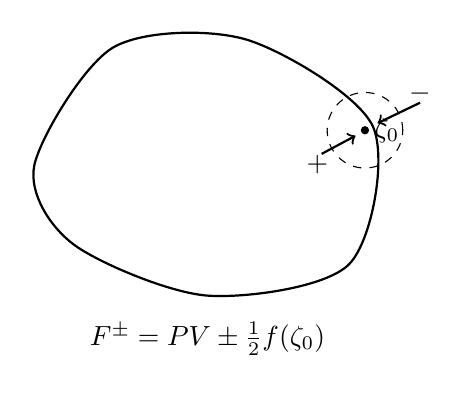
\begin{tikzpicture}[scale=1.0]
  \draw[thick] plot[smooth cycle] coordinates {(-2.2,0) (-1.2,1.5) (0.5,1.6) (2.1,0.5) (1.8,-1.25) (0,-1.65) (-1.7,-1.0)};
  \fill (2.0,0.45) circle (1.5pt) node[right] {$\zeta_0$};
  \draw[dashed] (2.0,0.45) circle (0.48);
  \draw[->,thick] (1.45,0.15)--(1.88,0.38) node[midway,below left] {$+$};
  \draw[->,thick] (2.7,0.8)--(2.16,0.54) node[midway,above right] {$-$};
  \node at (0,-2.2) {$F^\pm=\operatorname{PV}\pm\frac12 f(\zeta_0)$};
\end{tikzpicture}
\caption{The indentation method replaces a neighborhood of $\zeta_0$ by a small semicircular arc. Interior and exterior indentations contribute opposite half-residues, yielding the $\pm\frac12 f(\zeta_0)$ terms in the Sokhotski--Plemelj formulas.}
\label{fig:cp-iv-0106-plemelj-indentation}
\end{figure}


\begin{solution}
Let
\[
F(z)=\frac{1}{2\pi i}\int_\Gamma
\frac{f(\zeta)}{\zeta-z}\,d\zeta,
\qquad z\notin\Gamma.
\]
For \(z\) away from the contour, differentiation under the integral sign gives
\[
F'(z)
=
\frac{1}{2\pi i}
\int_\Gamma
\frac{f(\zeta)}{(\zeta-z)^2}\,d\zeta.
\]

Fix \(\zeta_0\in\Gamma\). Remove a symmetric small arc around \(\zeta_0\) and replace it by a small semicircular indentation. Split the integral into the integral over the truncated contour and the indentation. The first part tends to
\[
\operatorname{P.V.}\,
\frac{1}{2\pi i}
\int_\Gamma
\frac{f(\zeta)}{\zeta-\zeta_0}\,d\zeta.
\]
On the indentation,
\[
f(\zeta)=f(\zeta_0)+o(1),
\]
so its leading contribution is the integral of
\[
\frac{f(\zeta_0)}{\zeta-\zeta_0}.
\]
A half-turn contributes \(\pm\pi i\), with sign determined by the side and orientation. Dividing by \(2\pi i\) yields
\[
F^+(\zeta_0)
=
\frac12f(\zeta_0)
+
\operatorname{P.V.}\,
\frac{1}{2\pi i}\int_\Gamma
\frac{f(\zeta)}{\zeta-\zeta_0}\,d\zeta,
\]
and
\[
F^-(\zeta_0)
=
-\frac12f(\zeta_0)
+
\operatorname{P.V.}\,
\frac{1}{2\pi i}\int_\Gamma
\frac{f(\zeta)}{\zeta-\zeta_0}\,d\zeta.
\]
Hence
\[
F^+-F^-=f
\]
and
\[
\frac{F^++F^-}{2}
=
\operatorname{P.V.}\,
\frac{1}{2\pi i}\int_\Gamma
\frac{f(\zeta)}{\zeta-\zeta_0}\,d\zeta.
\]

For the unit circle and \(f(\zeta)=\zeta^m\), Cauchy's formula gives
\[
F(z)=
\begin{cases}
z^m,&|z|<1,\\
0,&|z|>1.
\end{cases}
\]
Therefore, at \(|\zeta_0|=1\),
\[
\operatorname{P.V.}\,
\frac{1}{2\pi i}
\int_{|\zeta|=1}
\frac{\zeta^m}{\zeta-\zeta_0}\,d\zeta
=
\frac12\zeta_0^m.
\]
\end{solution}


\begin{problem}[CP-IV-0116]
\label{prob:cp-iv-0116}
(Rotation–scaling; holomorphic).

Let $T(z)=\lambda z$ with $\lambda=1.3 e^{i\pi/6}$. Then $A=\lambda$, $B=0$.
The image of the unit circle is a circle of radius $1.3$ rotated by $\pi/6$, and $T$ preserves angles and orientation.
\end{problem}

\begin{solution}
Here
\[
T(z)=\lambda z,
\qquad
\lambda=1.3e^{i\pi/6}.
\]
Thus in the decomposition \(T(z)=Az+B\overline z\),
\[
A=\lambda,\qquad B=0.
\]
Hence \(T\) is complex-linear and therefore holomorphic.

If \(|z|=1\), then
\[
|T(z)|=|\lambda||z|=1.3,
\]
so the unit circle is mapped to the circle of radius \(1.3\). Moreover,
\[
\operatorname{Arg}T(z)
=
\operatorname{Arg}z+\frac{\pi}{6},
\]
so the image is rotated through \(\pi/6\).

The derivative is the nonzero constant
\[
T'(z)=\lambda,
\]
so the map is conformal. Its real Jacobian is
\[
|\lambda|^2=1.3^2>0,
\]
hence orientation is preserved.
\end{solution}


\begin{problem}[CP-IV-0117]
\label{prob:cp-iv-0117}
Let $f:\mathbb C\to\mathbb C$ be entire. Prove that $f$ is constant if any one of the following holds:

	\par\noindent\textbullet\quad $\displaystyle \frac{f(z)}{z}\to 0$ as $|z|\to\infty$.
	\par\noindent\textbullet\quad There exist $b\in\mathbb C$ and $\varepsilon>0$ such that $|f(z)-b|>\varepsilon$ for all $z\in\mathbb C$.
	\par\noindent\textbullet\quad Writing $f=u+iv$ with real $u,v$, one has $|u(z)|>|v(z)|$ for all $z\in\mathbb C$.

We use: (a) \emph{Liouville’s theorem}: a bounded entire function is constant; (b) \emph{Cauchy estimates}:
if $f$ is holomorphic on $|z|\le R$, then $|f^{(n)}(0)|\le \dfrac{n!}{R^n}\max_{|z|=R}|f(z)|$;
(c) the Cayley map $w\mapsto \dfrac{w-1}{w+1}$ sends $\{\Re w>0\}$ to the unit disk;
(d) if $FG\equiv 0$ with $F,G$ holomorphic on a connected set, then $F\equiv 0$ or $G\equiv 0$.
\end{problem}

\begin{solution}
\emph{(i) Sublinear growth.}
Given $\eta>0$, choose $R_\eta$ so that $|f(z)|\le \eta|z|$ for $|z|\ge R_\eta$.
For $R\ge R_\eta$,
\[
\max_{|z|=R}|f(z)|\le \eta R.
\]
Cauchy estimates at $0$ yield
\[
|f^{(n)}(0)|\le \frac{n!\,\eta R}{R^n}=\frac{n!\,\eta}{R^{n-1}}\quad(n\ge 1).
\]
Letting $R\to\infty$ gives $f^{(n)}(0)=0$ for $n\ge 2$, and $|f'(0)|\le \eta$ for all $\eta>0$, hence $f'(0)=0$.
Thus $f$ is constant.

\medskip
\emph{(ii) Image avoids a disk.}
If $|f(z)-b|>\varepsilon$ for all $z$, then $g(z)=\dfrac{1}{f(z)-b}$ is entire and bounded by $1/\varepsilon$.
By Liouville, $g$ is constant, hence $f$ is constant.

\medskip
\emph{(iii) Real part dominates.}
If $f=u+iv$ with $|u|>|v|$ everywhere, then $\Re\big(f^2\big)=u^2-v^2>0$, so $g:=f^2$ maps $\mathbb C$ into the right half–plane.
The Cayley transform $h=(g-1)/(g+1)$ is entire and satisfies $|h|<1$, hence $h$ is constant by Liouville, so $g\equiv c$ with $\Re c>0$.
Therefore $(f-\sqrt c)(f+\sqrt c)\equiv 0$, and by analyticity one factor vanishes identically.
Thus $f\equiv \sqrt c$ or $f\equiv -\sqrt c$, i.e. $f$ is constant.
\end{solution}

\begin{problem}[CP-IV-0126]
\label{prob:cp-iv-0126}
Let $U\subset\mathbb C$ be a domain and $u:U\to\mathbb R$ be $C^2$ and harmonic.
Show that if $z_0\in U$, then for any disk $D=D(z_0,r)\Subset U$ there exists a holomorphic
$f:D\to\mathbb C$ with $\Re f=u$ on $D$.
Show by an example that this need not hold globally.

\medskip

A $C^2$ real function $u$ is \emph{harmonic} if
\[
\Delta u \;=\; u_{xx}+u_{yy} \;=\; 0.
\]
Set the 1-form
\[
\alpha \;=\; -\,u_y\,dx \;+\; u_x\,dy.
\]
A short calculation gives
\[
d\alpha \;=\; (u_{xx}+u_{yy})\,dx\wedge dy \;=\; \Delta u\,dx\wedge dy.
\]
Hence if $u$ is harmonic, $\alpha$ is \emph{closed} ($d\alpha=0$).
On a simply connected domain (e.g.\ a disk), every closed 1-form is \emph{exact}, so there exists
$v$ with $dv=\alpha$, i.e.
\[
v_x=-u_y, \qquad v_y=u_x.
\]
Then the Cauchy–Riemann equations hold for $(u,v)$ and $f:=u+iv$ is holomorphic with $\Re f=u$.

\smallskip
On non–simply connected domains a closed form need not be exact; a certificate is a nonzero loop integral
\[
\oint_\gamma \alpha \;\neq\; 0
\qquad\text{for some closed curve }\gamma\subset U.
\]

\medskip
\end{problem}

% Designed Companion Part IV figure
% Intended for \input{...} beside the matching canonical problem.
\begin{figure}[ht]
\centering
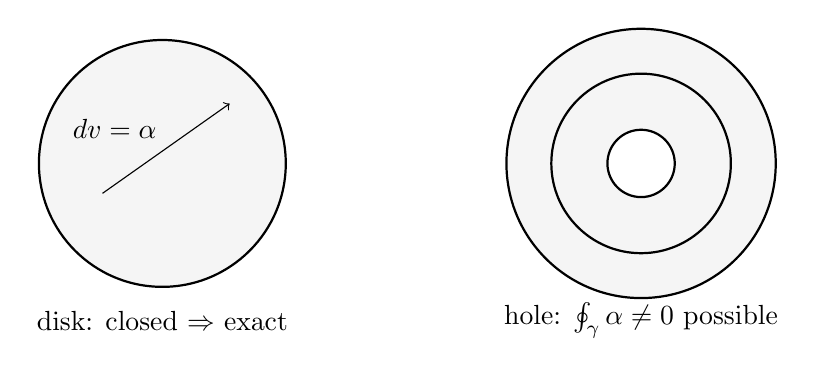
\begin{tikzpicture}[scale=0.95]
  \begin{scope}[xshift=-3.2cm]
    \fill[gray!8] (0,0) circle (1.65);
    \draw[thick] (0,0) circle (1.65);
    \draw[->] (-0.8,-0.4)--(0.9,0.8) node[midway,above left] {$dv=\alpha$};
    \node at (0,-2.1) {disk: closed $\Rightarrow$ exact};
  \end{scope}
  \begin{scope}[xshift=3.2cm]
    \fill[gray!8] (0,0) circle (1.8);
    \fill[white] (0,0) circle (0.45);
    \draw[thick] (0,0) circle (1.8);
    \draw[thick] (0,0) circle (0.45);
    \draw[->,thick] (0,0) circle (1.2);
    \node at (0,-2.1) {hole: $\oint_\gamma\alpha\ne0$ possible};
  \end{scope}
\end{tikzpicture}
\caption{For harmonic $u$, the conjugate differential $\alpha=-u_y\,dx+u_x\,dy$ is closed. On a disk it is exact and produces a harmonic conjugate; on a multiply connected domain a nonzero loop integral can obstruct a global conjugate.}
\label{fig:cp-iv-0126-harmonic-conjugate-local-global}
\end{figure}


\begin{solution}
\emph{Local existence on a disk.}
Fix $z_0\in U$ and $D=D(z_0,r)\Subset U$.
Since $u$ is harmonic, $d\alpha=0$ on $D$. Because $D$ is simply connected,
there exists $v:D\to\mathbb R$ with $dv=\alpha$, i.e.
\[
v_x=-u_y, \qquad v_y=u_x.
\]
Hence the Cauchy–Riemann equations hold and
\[
f:=u+iv \quad\text{is holomorphic on } D \text{ with } \Re f=u.
\]

\medskip
\emph{Failure globally: a counterexample.}
Let $U=\mathbb C\setminus\{0\}$ and $u(z)=\log|z|$. Then $u\in C^\infty(U)$ and $\Delta u=0$.
If there were a holomorphic $F$ on $U$ with $\Re F=u$, then its imaginary part $v=\Im F$
would satisfy $dv=\alpha=-u_y\,dx+u_x\,dy$.

\smallskip
On the unit circle $\gamma(t)=e^{it}$, $0\le t\le 2\pi$, one has
\[
u_x=\frac{x}{x^2+y^2}, \qquad u_y=\frac{y}{x^2+y^2},
\]
so along $|z|=1$,
\[
\oint_{\gamma}\alpha
=\oint_{\gamma}(-y\,dx+x\,dy)
=\int_0^{2\pi}\!\!\big(-\sin t\cdot(-\sin t)+\cos t\cdot\cos t\big)\,dt
=\int_0^{2\pi}\!1\,dt
=2\pi \;\neq\; 0.
\]
Thus $\alpha$ is not exact on $U$, so no global $v$ exists and $u$ is \emph{not}
the real part of any holomorphic function on $U$.
\end{solution}

\begin{problem}[CP-IV-0129]
\label{prob:cp-iv-0129}
\par\noindent\textbullet\quad \textbf{Pole:} $|f(z)|\to\infty$ as $z\to a$; equivalently, $(z-a)^m f(z)$ extends holomorphically with nonzero value at $a$ for some $m\in\mathbb N$.
\end{problem}

\begin{solution}
Suppose first that \(a\) is a pole of order \(m\). Then
\[
f(z)=\frac{g(z)}{(z-a)^m},
\]
where \(g\) is holomorphic near \(a\) and \(g(a)\neq0\). Hence
\[
(z-a)^m f(z)=g(z)
\]
extends holomorphically across \(a\) with a nonzero value there. In particular,
\[
|f(z)|=\frac{|g(z)|}{|z-a|^m}\longrightarrow\infty
\qquad (z\to a).
\]

Conversely, assume that for some \(m\ge1\),
\[
(z-a)^m f(z)
\]
extends holomorphically to \(a\) and has nonzero value there. Calling this extension \(g\), we have
\[
f(z)=\frac{g(z)}{(z-a)^m},
\qquad g(a)\neq0,
\]
so \(a\) is a pole of order exactly \(m\).

Equivalently, \(a\) is a pole precisely when \(1/f\) has a removable singularity at \(a\) whose extended value is \(0\). This is also equivalent to \(|f(z)|\to\infty\) as \(z\to a\).
\end{solution}


\begin{problem}[CP-IV-0133]
\label{prob:cp-iv-0133}
(Casorati--Weierstrass; restated).

If $f$ is holomorphic on $D(a,R)\setminus\{a\}$ with an essential singularity at $a$, then for any $b\in\mathbb C$
there exists a sequence $z_n\to a$ such that $f(z_n)\to b$.

\medskip
\end{problem}

\begin{solution}
\par\medskip\noindent\textbf{Solution to Problem 9.}\quad 
If $f$ omitted $b$ near $a$, then $g=1/(f-b)$ would be bounded near $a$, hence removable there by Riemann’s theorem.
Thus $f=b+1/g$ would have at worst a pole/removable singularity at $a$, contradicting essentiality.
\emph{Example.} For $f(z)=e^{1/z}$, $a=0$, $b=2$, take
\[
z_n=\frac{1}{\Log 2+2\pi i n}\quad\Rightarrow\quad e^{1/z_n}=2 .
\]

\bigskip
\end{solution}

\begin{problem}[CP-IV-0134]
\label{prob:cp-iv-0134}
\par\noindent\textbullet\quad \textbf{Isotropic:} conformality is equivalent to
	\[
	\phi_z\cdot \phi_z = 0
	\qquad\text{(complex bilinear dot product).}
	\]

\smallskip
\textbf{The holomorphic $\mathbb C^3$-valued $1$-form.}
Now set
\[
\Phi := 2\phi_z \in \mathbb C^3.
\]
Then $\Phi$ is a holomorphic map into $\mathbb C^3$ satisfying $\Phi\cdot \Phi=0$.
The $1$-form $\Phi\,dz$ is the holomorphic $\mathbb C^3$-valued form that one integrates to recover $\phi$:
\[
\Psi(z)=\int^z \Phi(\zeta)\,d\zeta \in \mathbb C^3,
\qquad
\phi(z)=\Re \Psi(z)\in \mathbb R^3.
\]

\smallskip
\textbf{Geometric meaning.}
The function $g$ is (up to stereographic projection) the Gauss map: it encodes the unit normal direction
$N\in\mathbb S^2$. Concretely,
\[
N
=
\frac{1}{1+|g|^2}\,\bigl(2\Re g,\ 2\Im g,\ |g|^2-1\bigr),
\]
which is inverse stereographic projection from $g\in\mathbb C$ to $N\in\mathbb S^2$.
The holomorphic $1$-form $f\,dz$ controls the conformal scale; the induced metric is
\[
ds^2
=
\frac{|f|^2(1+|g|^2)^2}{4}\,|dz|^2.
\]
Thus $|f|$ (together with $|g|$) determines local lengths; multiplying $f$ by $e^{-i\theta}$ rotates the differential but
does not change the metric.

\smallskip
\textbf{Clarifying the target spaces ($\mathbb C^3$ vs.\ $\mathbb R^3$ vs.\ $\mathbb C^2$).}
\end{problem}

\begin{solution}
Let \(z=u+iv\) be a conformal parameter for the minimal immersion
\[
\phi:\Omega\longrightarrow\mathbb R^3.
\]
Write
\[
\phi_z=\frac12(\phi_u-i\phi_v).
\]
Conformality means
\[
\langle\phi_u,\phi_u\rangle=\langle\phi_v,\phi_v\rangle,
\qquad
\langle\phi_u,\phi_v\rangle=0.
\]
Therefore, using the complex bilinear extension of the Euclidean dot product,
\[
\phi_z\cdot\phi_z
=
\frac14\bigl(
|\phi_u|^2-|\phi_v|^2-2i\,\phi_u\cdot\phi_v
\bigr)
=0.
\]
Thus conformality is equivalent to the isotropy condition
\[
\boxed{\phi_z\cdot\phi_z=0}.
\]

Minimality in conformal coordinates is equivalent to harmonicity of the coordinate functions, hence
\[
\phi_{z\bar z}=0.
\]
Consequently
\[
\Phi:=2\phi_z:\Omega\to\mathbb C^3
\]
is holomorphic and satisfies
\[
\Phi\cdot\Phi=0.
\]
On a simply connected domain,
\[
\Psi(z)=\int^z\Phi(\zeta)\,d\zeta\in\mathbb C^3
\]
is holomorphic and
\[
\phi=\Re\Psi.
\]

With Weierstrass data \((f,g)\),
\[
\Phi
=
\left(
\frac12f(1-g^2),
\frac{i}{2}f(1+g^2),
fg
\right).
\]
The meromorphic function \(g\) is the stereographic coordinate of the Gauss map:
\[
N=
\frac{1}{1+|g|^2}
\bigl(2\Re g,\,2\Im g,\,|g|^2-1\bigr).
\]
The \(1\)-form \(f\,dz\) controls the conformal scale, since
\[
ds^2=\frac{|f|^2(1+|g|^2)^2}{4}|dz|^2.
\]

Thus the roles of the target spaces are distinct: \(\Phi\) and \(\Psi\) take values in \(\mathbb C^3\), while the actual surface \(\phi=\Re\Psi\) takes values in \(\mathbb R^3\). The pair \((f,g)\) is scalar holomorphic/meromorphic data, not a map into \(\mathbb C^2\) representing the surface directly.
\end{solution}


\section{Singularities and Residues}

\par\medskip\noindent\textbf{Related material.}\quad Volume IV, Chapters \texttt{IV/07--IV/11}.

\begin{problem}[CP-IV-0024]
\label{prob:cp-iv-0024}
Consider the meromorphic function
	\[
	F(z) = \frac{1}{1+z^2} \frac{\cos[(\pi-\theta)z]}{2\sin(\pi z)}.
	\]

	The poles occur at $z=\pm i$ and $z=n$, $n\in\mathbb{Z}$.
	At $z=\pm i$:
	\[
	\operatorname{Res}[F,\pm i] = -\frac{\cosh(\pi-\theta)}{4\sinh \pi}.
	\]
	At $z=n\in\mathbb{Z}$:
	\[
	\operatorname{Res}[F,n] = \frac{\cos(n\theta)}{2\pi(1+n^2)}.
	\]

	\subsection*{b) The contour $\Gamma^{(N)}$}
	Define
	\[
	\Gamma^{(N)}_1(t) = \Big(N+\tfrac{1}{2}\Big)(1+it), \quad -1\leq t\leq 1,
	\]
	\[
	\Gamma^{(N)}_2(t) = \Big(N+\tfrac{1}{2}\Big)(-t+i), \quad -1\leq t\leq 1,
	\]
	\[
	\Gamma^{(N)}_3(t) = \Big(N+\tfrac{1}{2}\Big)(-1-it), \quad -1\leq t\leq 1,
	\]
	\[
	\Gamma^{(N)}_4(t) = \Big(N+\tfrac{1}{2}\Big)(t-i), \quad -1\leq t\leq 1.
	\]
	Then $\Gamma^{(N)}$ is the closed square contour with vertices
	$\pm(N+\tfrac{1}{2}) \pm i(N+\tfrac{1}{2})$.
	It encloses the poles at $\pm i$ and all integers $n$ with $|n|\leq N$.

	On $\Gamma^{(N)}$, $|z|\sim N$, so $|F(z)|=O(1/N^2)$.
	Since the contour has length $O(N)$, we obtain
	\[
	\left| \int_{\Gamma^{(N)}} F(z)\,dz \right| \leq \frac{C}{N},
	\]
	for some constant $C$ independent of $N$.

	By Cauchy's residue theorem,
	\[
	\int_{\Gamma^{(N)}} F(z)\,dz
	= 2\pi i \left( \operatorname{Res}[F,i]+\operatorname{Res}[F,-i] + \sum_{n=-N}^N \operatorname{Res}[F,n]\right).
	\]
	Hence
	\[
	\left| \frac{\cosh(\pi-\theta)}{2\sinh \pi}
	- \sum_{n=-N}^N \frac{\cos(n\theta)}{1+n^2} \right| \leq \frac{C}{N}.
	\]
	Letting $N\to\infty$, we conclude
	\[
	\frac{\cosh(\pi-\theta)}{2\sinh \pi}
	= \sum_{n=-\infty}^\infty \frac{e^{in\theta}}{1+n^2}.
	\]

	This gives the Fourier series expansion, uniformly in $\theta$.
\end{problem}

% Designed Companion Part IV figure
% Intended for \input{...} beside the matching canonical problem.
\begin{figure}[ht]
\centering
\begin{tikzpicture}[scale=0.88]
  \draw[->] (-4.2,0)--(4.2,0) node[right] {$\Re z$};
  \draw[->] (0,-3.2)--(0,3.2) node[above] {$\Im z$};
  \draw[thick] (-3.4,-2.7) rectangle (3.4,2.7);
  \foreach \x in {-3,-2,-1,0,1,2,3} {\fill (\x,0) circle (1.4pt);}
  \fill (0,1) circle (1.6pt) node[right] {$i$};
  \fill (0,-1) circle (1.6pt) node[right] {$-i$};
  \node at (2.7,2.25) {$\Gamma^{(N)}$};
\end{tikzpicture}
\caption{The square contour $\Gamma^{(N)}$ encloses the integer poles with $|n|\le N$ together with the poles at $\pm i$. The half-integer boundary keeps the contour away from the integer poles.}
\label{fig:cp-iv-0024-square-residue-contour}
\end{figure}


\begin{solution}
The poles of
\[
F(z)=\frac{1}{1+z^2}\,
\frac{\cos((\pi-\theta)z)}{2\sin(\pi z)}
\]
are \(z=\pm i\) and the integers.

At \(z=i\),
\[
\operatorname{Res}(F;i)
=
\frac{1}{2i}\,
\frac{\cosh(\pi-\theta)}{2i\sinh\pi}
=
-\frac{\cosh(\pi-\theta)}{4\sinh\pi},
\]
and the same value is obtained at \(z=-i\).

At an integer \(n\),
\[
\sin(\pi z)=\pi(-1)^n(z-n)+O((z-n)^2),
\]
while
\[
\cos((\pi-\theta)n)=(-1)^n\cos(n\theta).
\]
Hence
\[
\operatorname{Res}(F;n)
=
\frac{\cos(n\theta)}{2\pi(1+n^2)}.
\]

Let \(\Gamma_N\) be the square with vertices
\[
\pm\left(N+\frac12\right)
\pm i\left(N+\frac12\right).
\]
On its vertical sides, \(|\sin(\pi z)|\) is bounded away from zero, while on its horizontal sides it grows exponentially at the same rate as the numerator. Together with
\[
|1+z^2|^{-1}=O(N^{-2})
\]
and \(\operatorname{length}(\Gamma_N)=O(N)\), this gives
\[
\left|\int_{\Gamma_N}F(z)\,dz\right|=O(N^{-1}).
\]

The residue theorem yields
\[
\frac{1}{2\pi i}\int_{\Gamma_N}F(z)\,dz
=
-\frac{\cosh(\pi-\theta)}{2\sinh\pi}
+
\frac{1}{2\pi}
\sum_{n=-N}^{N}\frac{\cos(n\theta)}{1+n^2}.
\]
Letting \(N\to\infty\),
\[
\boxed{
\sum_{n\in\mathbb Z}\frac{\cos(n\theta)}{1+n^2}
=
\pi\,\frac{\cosh(\pi-\theta)}{\sinh\pi},
\qquad 0\le\theta\le2\pi.
}
\]
Because the summand is even in \(n\),
\[
\sum_{n\in\mathbb Z}\frac{e^{in\theta}}{1+n^2}
=
\sum_{n\in\mathbb Z}\frac{\cos(n\theta)}{1+n^2},
\]
so the same formula holds with \(e^{in\theta}\).

With the normalization of \(F\) printed in the problem, the factor \(\pi\) in this final identity is necessary; any displayed target omitting it has a normalization mismatch.
\end{solution}


\begin{problem}[CP-IV-0025]
\label{prob:cp-iv-0025}
Classify the singularities of
\[
\frac{z}{\sin z},\qquad
\sin\!\Big(\frac{\pi}{z^{2}}\Big),\qquad
\frac{1}{z^{2}}+\frac{1}{z^{2}+1},\qquad
\frac{1}{z^{2}}\cos\!\Big(\frac{\pi z}{z+1}\Big).
\]

At an isolated singularity $a$, if the Laurent expansion
$f(z)=\sum_{k=-m}^{\infty} c_k (z-a)^k$ has
(i) $m=0$ $\Rightarrow$ removable;
(ii) finitely many negative terms with highest $(z-a)^{-m}$ $\Rightarrow$ pole of order $m$;
(iii) infinitely many negative terms $\Rightarrow$ essential.

\medskip
\emph{(1) $\boldsymbol{z/\sin z}$.}
Near $0$, $\sin z=z-\frac{z^{3}}{6}+O(z^{5})$, so
\[
\frac{z}{\sin z}=1+\frac{z^{2}}{6}+O(z^{4}),
\]
hence $z=0$ is \textbf{removable} (define value $1$). At $z=n\pi$, $n\in\mathbb Z\setminus\{0\}$,
$\sin z$ has simple zeros and the numerator is nonzero, so each $n\pi$ is a \textbf{simple pole}.

\medskip
\emph{(2) $\boldsymbol{\sin(\pi/z^{2})}$.}
Using $\sin w=\sum_{k\ge0}\frac{(-1)^k w^{2k+1}}{(2k+1)!}$ with $w=\pi/z^{2}$,
\[
\sin\!\Big(\frac{\pi}{z^{2}}\Big)=\sum_{k=0}^{\infty}\frac{(-1)^k \pi^{2k+1}}{(2k+1)!}\,z^{-4k-2},
\]
which contains infinitely many negative powers. Thus $z=0$ is an \textbf{essential singularity}.
There are no other singularities.

\medskip
\emph{(3) $\boldsymbol{1/z^{2} + 1/(z^{2}+1)}$.}
At $z=0$ one has a \textbf{pole of order $2$}. At $z=\pm i$ (simple zeros of $z^{2}+1$) there are
\textbf{simple poles}. No other singularities occur.

\medskip
\emph{(4) $\boldsymbol{z^{-2}\cos\!\big(\pi z/(z+1)\big)}$.}
Let $h(z)=\dfrac{\pi z}{z+1}$.
Near $z=0$, $h(z)=\pi(z-z^{2}+z^{3}-\cdots)$, hence
\[
\cos h(z)=1-\tfrac12 h(z)^{2}+O(z^{3})=1-\tfrac{\pi^{2}}{2}z^{2}+O(z^{3}),
\]
and
\[
\frac{1}{z^{2}}\cos h(z)=\frac{1}{z^{2}}-\frac{\pi^{2}}{2}+O(z),
\]
so $z=0$ is a \textbf{pole of order $2$}. At $z=-1$, $h$ has a simple pole; since
$\cos w=\tfrac12(e^{iw}+e^{-iw})$, composition with a pole yields an \textbf{essential singularity}
at $z=-1$. There are no other singularities.

\end{problem}

\begin{solution}
For
\[
f_1(z)=\frac{z}{\sin z},
\]
the point \(0\) is removable because
\[
\sin z=z-\frac{z^3}{6}+O(z^5),
\qquad
\frac{z}{\sin z}=1+\frac{z^2}{6}+O(z^4).
\]
Every nonzero \(n\pi\) is a simple pole, since \(\sin z\) has a simple zero there and the numerator does not vanish.

For
\[
f_2(z)=\sin\!\left(\frac{\pi}{z^2}\right),
\]
the Laurent expansion at \(0\) is
\[
\sum_{k=0}^{\infty}
\frac{(-1)^k\pi^{2k+1}}{(2k+1)!}\,z^{-4k-2}.
\]
It contains infinitely many negative powers, so \(0\) is an essential singularity.

For
\[
f_3(z)=\frac1{z^2}+\frac1{z^2+1},
\]
\(z=0\) is a pole of order \(2\), while \(z=\pm i\) are simple poles.

Finally, let
\[
f_4(z)=\frac1{z^2}
\cos\!\left(\frac{\pi z}{z+1}\right).
\]
Near \(0\),
\[
\frac{\pi z}{z+1}=\pi z+O(z^2),
\]
hence
\[
\cos\!\left(\frac{\pi z}{z+1}\right)
=
1-\frac{\pi^2z^2}{2}+O(z^3),
\]
so
\[
f_4(z)=\frac1{z^2}-\frac{\pi^2}{2}+O(z),
\]
and \(0\) is a pole of order \(2\).

At \(z=-1\), the inner function \(\pi z/(z+1)\) has a pole. Since
\[
\cos w=\frac{e^{iw}+e^{-iw}}2
\]
is transcendental entire, its composition with a pole has an essential singularity. Thus \(z=-1\) is essential.

These are all the finite singularities.
\end{solution}


\begin{problem}[CP-IV-0029]
\label{prob:cp-iv-0029}
(Cauchy’s derivative formula via residues).

Let $f$ be holomorphic on $D(a,R)$. If $w$ satisfies $|w-a|<r<R$, show
\[
f^{(n)}(w)=\frac{n!}{2\pi i}\int_{|z-a|=r}\frac{f(z)}{(z-w)^{n+1}}\,dz.
\]

\emph{Residue at a higher–order pole.}
If $g$ has a pole of order $m$ at $w$,
\[
\operatorname{Res}(g;w)=\frac{1}{(m-1)!}\lim_{z\to w}\frac{d^{\,m-1}}{dz^{m-1}}\Big((z-w)^m g(z)\Big).
\]
\emph{Residue theorem.}
If $g$ is meromorphic on and inside a positively oriented simple closed curve $\gamma$ (no poles on $\gamma$),
\[
\int_\gamma g(z)\,dz=2\pi i\sum \operatorname{Res}(g;a_k).
\]
\emph{Taylor series at $w$.}
For $f$ holomorphic near $w$,
\[
f(z)=\sum_{k=0}^{\infty}\frac{f^{(k)}(w)}{k!}(z-w)^k .
\]

\medskip
\end{problem}

% Designed Companion Part IV figure
% Intended for \input{...} beside the matching canonical problem.
\begin{figure}[ht]
\centering
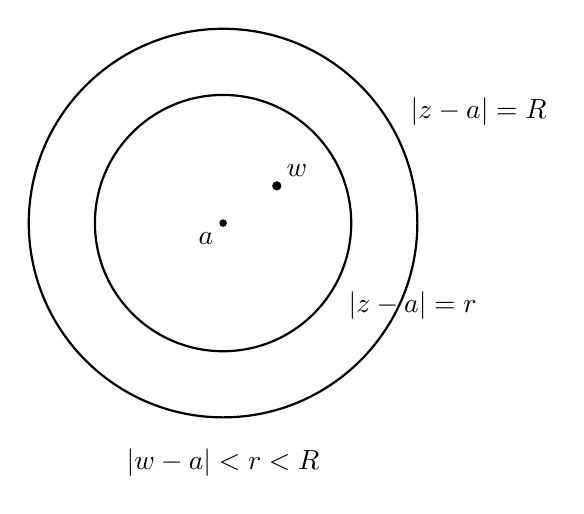
\begin{tikzpicture}[scale=1.05]
  \draw[thick] (0,0) circle (2.35);
  \draw[thick] (0,0) circle (1.55);
  \fill (0,0) circle (1.3pt) node[below left] {$a$};
  \fill (0.65,0.45) circle (1.6pt) node[above right] {$w$};
  \node[right] at (2.15,1.35) {$|z-a|=R$};
  \node[right] at (1.4,-1.0) {$|z-a|=r$};
  \node at (0,-2.9) {$|w-a|<r<R$};
\end{tikzpicture}
\caption{Cauchy's derivative formula integrates on the inner circle $|z-a|=r$, while the evaluation point $w$ lies strictly inside and the function is holomorphic on the larger disk $D(a,R)$.}
\label{fig:cp-iv-0029-cauchy-derivative-nested-disks}
\end{figure}


\begin{solution}
Put $g(z)=\dfrac{f(z)}{(z-w)^{n+1}}$. Then $g$ is meromorphic on $|z-a|\le r$, with a single pole at $z=w$ of order $n+1$.
Hence
\[
\operatorname{Res}(g;w)=\frac{1}{n!}\,f^{(n)}(w).
\]
By the residue theorem on $|z-a|=r$,
\[
\int_{|z-a|=r}\frac{f(z)}{(z-w)^{n+1}}\,dz
= 2\pi i\,\operatorname{Res}(g;w)
= 2\pi i\,\frac{f^{(n)}(w)}{n!},
\]
which yields the claimed formula. For $n=0$ this reduces to Cauchy’s integral formula.

\medskip
\end{solution}

\begin{problem}[CP-IV-0048]
\label{prob:cp-iv-0048}
— area from a $1$-form (what $\tfrac12(x\,dy-y\,dx)$ measures)

Set
\[
\alpha \;=\; \frac12\,(x\,dy - y\,dx).
\]
Then
\[
d\alpha
=
\frac12\,(dx\wedge dy + dy\wedge dx)
=
dx\wedge dy.
\]
Hence, by Stokes/Green,
\[
\oint_{C} \alpha
=
\iint_{D} dx\wedge dy
=
\operatorname{Area}(D)
=
\pi R^2.
\]
Therefore,
\[
\boxed{\ \frac12 \oint_{C} (x\,dy - y\,dx)\;=\;\operatorname{Area}(D)\;=\;\pi R^2\ }.
\]

	\par\noindent\textbullet\quad Pick $\mathbf F=(L,M)$ $\Rightarrow$ $1$-form $L\,dx+M\,dy$.
	\par\noindent\textbullet\quad Circulation (line integral on $C$) equals total curl over $D$.
	\par\noindent\textbullet\quad If $\;M_x-L_y\equiv 0$ on $D$, then $\displaystyle \oint_{C}(L\,dx+M\,dy)=0$ (path-independence on simply connected $D$).
	\par\noindent\textbullet\quad The special $1$-form $\tfrac12(x\,dy - y\,dx)$ integrates to the enclosed area.
\end{problem}

\begin{solution}
Set
\[
\alpha=\frac12(x\,dy-y\,dx).
\]
Then
\[
d\alpha
=
\frac12(dx\wedge dy-dy\wedge dx)
=
dx\wedge dy.
\]
If \(C=\partial D\) is positively oriented, Green's theorem gives
\[
\oint_C\alpha
=
\iint_D d\alpha
=
\iint_D dx\,dy
=
\operatorname{Area}(D).
\]
Therefore
\[
\boxed{
\frac12\oint_C(x\,dy-y\,dx)=\operatorname{Area}(D).
}
\]
For a circle of radius \(R\), this equals
\[
\pi R^2.
\]

More generally, for a \(1\)-form
\[
\omega=L\,dx+M\,dy,
\]
Green's theorem says
\[
\oint_C\omega
=
\iint_D(M_x-L_y)\,dx\,dy.
\]
Thus a closed \(1\)-form has zero integral around every closed curve in a simply connected domain, and the special form above measures oriented area.
\end{solution}


\begin{problem}[CP-IV-0053]
\label{prob:cp-iv-0053}
Consider the meromorphic function
\[
F(z) = \frac{1}{1+z^2} \frac{\cos[(\pi-\theta)z]}{2\sin(\pi z)}.
\]

The poles occur at $z=\pm i$ and $z=n$, $n\in\mathbb{Z}$.
At $z=\pm i$:
\[
\operatorname{Res}[F,\pm i] = -\frac{\cosh(\pi-\theta)}{4\sinh \pi}.
\]
At $z=n\in\mathbb{Z}$:
\[
\operatorname{Res}[F,n] = \frac{\cos(n\theta)}{2\pi(1+n^2)}.
\]

\subsection*{b) The contour $\Gamma^{(N)}$}
Define
\[
\Gamma^{(N)}_1(t) = \Big(N+\tfrac{1}{2}\Big)(1+it), \quad -1\leq t\leq 1,
\]
\[
\Gamma^{(N)}_2(t) = \Big(N+\tfrac{1}{2}\Big)(-t+i), \quad -1\leq t\leq 1,
\]
\[
\Gamma^{(N)}_3(t) = \Big(N+\tfrac{1}{2}\Big)(-1-it), \quad -1\leq t\leq 1,
\]
\[
\Gamma^{(N)}_4(t) = \Big(N+\tfrac{1}{2}\Big)(t-i), \quad -1\leq t\leq 1.
\]
Then $\Gamma^{(N)}$ is the closed square contour with vertices
$\pm(N+\tfrac{1}{2}) \pm i(N+\tfrac{1}{2})$.
It encloses the poles at $\pm i$ and all integers $n$ with $|n|\leq N$.

On $\Gamma^{(N)}$, $|z|\sim N$, so $|F(z)|=O(1/N^2)$.
Since the contour has length $O(N)$, we obtain
\[
\left| \int_{\Gamma^{(N)}} F(z)\,dz \right| \leq \frac{C}{N},
\]
for some constant $C$ independent of $N$.

By Cauchy's residue theorem,
\[
\int_{\Gamma^{(N)}} F(z)\,dz
= 2\pi i \left( \operatorname{Res}[F,i]+\operatorname{Res}[F,-i] + \sum_{n=-N}^N \operatorname{Res}[F,n]\right).
\]
Hence
\[
\left| \frac{\cosh(\pi-\theta)}{2\sinh \pi}
- \sum_{n=-N}^N \frac{\cos(n\theta)}{1+n^2} \right| \leq \frac{C}{N}.
\]
Letting $N\to\infty$, we conclude
\[
\frac{\cosh(\pi-\theta)}{2\sinh \pi}
= \sum_{n=-\infty}^\infty \frac{e^{in\theta}}{1+n^2}.
\]

This gives the Fourier series expansion, uniformly in $\theta$.
\end{problem}

% Designed Companion Part IV figure
% Intended for \input{...} beside the matching canonical problem.
\begin{figure}[ht]
\centering
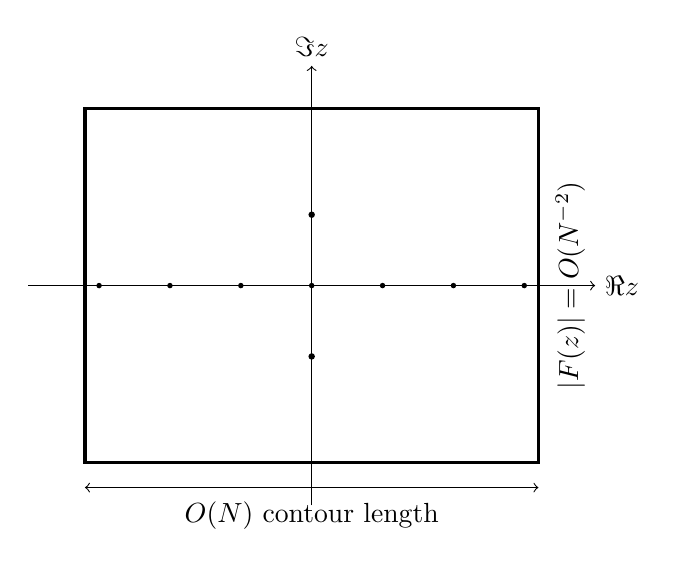
\begin{tikzpicture}[scale=0.9]
  \draw[->] (-4,0)--(4,0) node[right] {$\Re z$};
  \draw[->] (0,-3.1)--(0,3.1) node[above] {$\Im z$};
  \draw[very thick] (-3.2,-2.5) rectangle (3.2,2.5);
  \draw[<->] (-3.2,-2.85)--(3.2,-2.85);
  \node at (0,-3.25) {$O(N)$ contour length};
  \node[rotate=90] at (3.65,0) {$|F(z)|=O(N^{-2})$};
  \foreach \x in {-3,-2,-1,0,1,2,3} \fill (\x,0) circle (1.1pt);
  \fill (0,1) circle (1.3pt);
  \fill (0,-1) circle (1.3pt);
\end{tikzpicture}
\caption{On the large square contour the kernel is $O(N^{-2})$ while the contour length is $O(N)$, yielding the uniform estimate $\left|\int_{\Gamma^{(N)}}F(z)\,dz\right|=O(N^{-1})$.}
\label{fig:cp-iv-0053-residue-contour-estimate}
\end{figure}


\begin{solution}
The residue computation is the same for
\[
F(z)=\frac{1}{1+z^2}\,
\frac{\cos((\pi-\theta)z)}{2\sin(\pi z)}.
\]
The simple poles are \(z=\pm i\) and \(z=n\in\mathbb Z\), with
\[
\operatorname{Res}(F;\pm i)
=
-\frac{\cosh(\pi-\theta)}{4\sinh\pi},
\qquad
\operatorname{Res}(F;n)
=
\frac{\cos(n\theta)}{2\pi(1+n^2)}.
\]

Integrating over the half-integer square \(\Gamma_N\), one has
\[
\int_{\Gamma_N}F(z)\,dz\longrightarrow0,
\]
because the contour length is \(O(N)\) and \(F(z)=O(N^{-2})\) uniformly on the boundary after the standard sine/cosine estimates.

Hence
\[
0
=
-\frac{\cosh(\pi-\theta)}{2\sinh\pi}
+
\frac{1}{2\pi}
\sum_{n\in\mathbb Z}\frac{\cos(n\theta)}{1+n^2},
\]
and therefore
\[
\boxed{
\sum_{n\in\mathbb Z}\frac{e^{in\theta}}{1+n^2}
=
\pi\frac{\cosh(\pi-\theta)}{\sinh\pi}.
}
\]
The convergence is uniform in \(\theta\), since
\[
\sum_{n\in\mathbb Z}\frac1{1+n^2}<\infty
\]
and the Weierstrass \(M\)-test applies directly.

Thus, with the normalization used in the problem, the mathematically consistent Fourier identity contains the factor \(\pi\).
\end{solution}


\begin{problem}[CP-IV-0062]
\label{prob:cp-iv-0062}
\par\noindent\textbullet\quad Define
	\[
	g(z):=f(z)-z .
	\]
	Then $g$ is entire and $g(1/n)=0$ for all $n$. Since $1/n\to 0$ (an interior point),
	the identity theorem gives $g\equiv 0$, hence $f(z)\equiv z$.

	\medskip
\end{problem}

\begin{solution}
Define
\[
g(z)=f(z)-z.
\]
Then \(g\) is entire and
\[
g(1/n)=0
\qquad (n\ge1).
\]
The zeros \(1/n\) accumulate at \(0\), and \(0\) is an interior point of the domain of \(g\). By the identity theorem,
\[
g\equiv0.
\]
Consequently
\[
\boxed{f(z)=z\quad\text{for all }z\in\mathbb C.}
\]
\end{solution}


\begin{problem}[CP-IV-0070]
\label{prob:cp-iv-0070}
\par\noindent\textbullet\quad Show that $F$ has poles at $z=\pm i$ and at each integer $z=n$, $n\in\mathbb{Z}$. Compute the residues at these poles and verify that
	\[
	\operatorname{Res}(F,\pm i)
	= -\frac{\cosh(\pi-\theta)}{4\sinh\pi},
	\qquad
	\operatorname{Res}(F,n)
	= \frac{\cos(n\theta)}{2\pi\,(1+n^2)}.
	\]

	\par\noindent\textbullet\quad For each $N\in\mathbb{N}$ define four curves $\Gamma^{(N)}_j$ on $[-1,1]$ by
	\[
	\Gamma^{(N)}_1(t) = \Bigl(N+\tfrac12\Bigr)(1+it),\qquad
	\Gamma^{(N)}_2(t) = \Bigl(N+\tfrac12\Bigr)(-t+i),
	\]
	\[
	\Gamma^{(N)}_3(t) = \Bigl(N+\tfrac12\Bigr)(-1-it),\qquad
	\Gamma^{(N)}_4(t) = \Bigl(N+\tfrac12\Bigr)(t-i),
	\]
	and let $\Gamma^{(N)}$ be the closed contour obtained by following
	$\Gamma^{(N)}_1,\Gamma^{(N)}_2,\Gamma^{(N)}_3,\Gamma^{(N)}_4$ in turn.
	Sketch $\Gamma^{(N)}$ in the complex plane and indicate the locations of the poles of $F$ relative to this rectangle.

	\par\noindent\textbullet\quad Show that there exists a constant $C>0$, independent of $N$, such that for all integers $N\ge 1$ and all $\theta\in[0,2\pi]$,
	\[
	\left| \int_{\Gamma^{(N)}} F(z)\,dz \right|
	\le \frac{C}{N}.
	\]

	\par\noindent\textbullet\quad Using Cauchy’s residue theorem applied to $\Gamma^{(N)}$, show that for $0\le\theta\le 2\pi$,
	\[
	\left|
	\frac{\cosh(\pi-\theta)}{2\sinh\pi}
	- \sum_{n=-N}^N \frac{e^{in\theta}}{1+n^2}
	\right|
	\le \frac{C}{N},
	\]
	and deduce that
	\[
	\frac{\cosh(\pi-\theta)}{2\sinh\pi}
	= \sum_{n=-\infty}^{\infty} \frac{e^{in\theta}}{1+n^2},
	\]
	with the series converging uniformly in $\theta\in[0,2\pi]$.

The function $F$ is meromorphic on $\mathbb{C}$, being the product of the entire function
$\cos\bigl((\pi-\theta)z\bigr)$ with the factors $(1+z^2)^{-1}$ and $(\sin\pi z)^{-1}$.
The only singularities of $F$ are poles arising from zeros of $1+z^2$ and $\sin(\pi z)$.

The equation $1+z^2=0$ has solutions $z=\pm i$, which give simple poles of $F$.
The function $\sin(\pi z)$ vanishes simply at each integer $z=n\in\mathbb{Z}$, so
$(\sin\pi z)^{-1}$ has simple poles there. Since $1+z^2$ does not vanish at any integer,
$F$ also has simple poles at all $z=n\in\mathbb{Z}$.

For a simple pole at $a\in\mathbb{C}$, the residue is given by
\[
\operatorname{Res}(F,a) = \lim_{z\to a} (z-a)\,F(z).
\]
At an integer $n$ one uses the local behaviour
$\sin(\pi z) = \pi(-1)^n(z-n) + O\bigl((z-n)^2\bigr)$ and evaluates the remaining factors at $z=n$.
At $z=\pm i$ one factors $1+z^2=(z-i)(z+i)$ and again evaluates the remaining analytic part at the pole.

The contour $\Gamma^{(N)}$ is a rectangle with vertices
\[
\pm\Bigl(N+\tfrac12\Bigr)\pm i,
\]
with horizontal sides at $\Im z=\pm1$ and vertical sides at $\Re z=\pm(N+\tfrac12)$.
For each fixed $N$, the contour encloses the poles at $z=\pm i$ and at the integers $n$ with $|n|\le N$.

Cauchy’s residue theorem states that for such a closed contour,
\[
\int_{\Gamma^{(N)}} F(z)\,dz
= 2\pi i \sum_{a\in\mathcal{P}_N} \operatorname{Res}(F,a),
\]
where $\mathcal{P}_N$ is the finite set of poles of $F$ inside $\Gamma^{(N)}$.
Here $\mathcal{P}_N=\{-i,+i\}\cup\{n\in\mathbb{Z}:|n|\le N\}$.

To estimate the integral along $\Gamma^{(N)}$ one uses the estimation lemma
\[
\left|\int_{\Gamma^{(N)}} F(z)\,dz\right|
\le \sup_{z\in\Gamma^{(N)}} |F(z)|\cdot \operatorname{length}(\Gamma^{(N)}).
\]
On the vertical segments, $z = \pm\bigl(N+\tfrac12\bigr) + it$ with $-1\le t\le 1$, the factor
$1/(1+z^2)$ is of order $1/N^2$, whereas $\cos\bigl((\pi-\theta)z\bigr)$ and
$1/\sin(\pi z)$ are uniformly bounded in $N$, since $\Im z$ stays in a compact set.
On the horizontal segments, $\Re z$ is bounded and $\Im z=\pm1$, so $F$ remains uniformly bounded.
Combining these facts gives a bound of the form
\[
\left|\int_{\Gamma^{(N)}} F(z)\,dz\right|
\le \frac{C}{N}
\]
for some constant $C$ independent of $N$ and $\theta$.

Substituting the residue computations into the residue theorem gives an identity of the form
\[
\frac{\cosh(\pi-\theta)}{2\sinh\pi}
- \sum_{n=-N}^N \frac{e^{in\theta}}{1+n^2}
= \frac{1}{2\pi i}\int_{\Gamma^{(N)}} F(z)\,dz,
\]
so that the absolute value of the difference is bounded by $C/N$.
Letting $N\to\infty$ shows that the Fourier series
\[
\sum_{n=-\infty}^{\infty} \frac{e^{in\theta}}{1+n^2}
\]
converges uniformly in $\theta\in[0,2\pi]$ and represents $\cosh(\pi-\theta)/(2\sinh\pi)$.
\end{problem}

% Designed Companion Part IV figure
% Intended for \input{...} beside the matching canonical problem.
\begin{figure}[ht]
\centering
\begin{tikzpicture}[scale=0.88]
  \draw[->] (-4.1,0)--(4.1,0) node[right] {$\Re z$};
  \draw[->] (0,-3.1)--(0,3.1) node[above] {$\Im z$};
  \draw[thick,->] (3.4,-2.6)--(3.4,2.6)--(-3.4,2.6)--(-3.4,-2.6)--(3.4,-2.6);
  \foreach \x in {-3,-2,-1,0,1,2,3} {\fill (\x,0) circle (1.4pt);}
  \fill (0,1) circle (1.7pt) node[right] {$+i$};
  \fill (0,-1) circle (1.7pt) node[right] {$-i$};
  \node at (2.5,2.2) {$\Gamma^{(N)}$};
\end{tikzpicture}
\caption{The residue theorem reduces the contour integral to the finite pole set $\mathcal P_N=\{-i,+i\}\cup\{n\in\mathbb Z:|n|\le N\}$ inside the half-integer square.}
\label{fig:cp-iv-0070-residue-inventory-square}
\end{figure}


\begin{solution}
The singularities of
\[
F(z)=\frac{1}{1+z^2}\,
\frac{\cos((\pi-\theta)z)}{2\sin(\pi z)}
\]
are the simple poles \(z=\pm i\) and \(z=n\in\mathbb Z\). Their residues are
\[
\operatorname{Res}(F;\pm i)
=
-\frac{\cosh(\pi-\theta)}{4\sinh\pi},
\qquad
\operatorname{Res}(F;n)
=
\frac{\cos(n\theta)}{2\pi(1+n^2)}.
\]

The four parametrized sides in the problem form the square
\[
\Gamma_N:
\qquad
|\Re z|\le N+\frac12,\qquad
|\Im z|\le N+\frac12.
\]
Thus its vertices are
\[
\pm\left(N+\frac12\right)
\pm i\left(N+\frac12\right),
\]
and it contains \(\pm i\) and the integers \(|n|\le N\).

On the vertical sides, \(\Re z=\pm(N+\tfrac12)\), the sine denominator is bounded away from zero after comparison with the hyperbolic terms. On the horizontal sides, numerator and sine denominator have the same exponential scale. Since
\[
|1+z^2|^{-1}=O(N^{-2})
\]
and the perimeter is \(O(N)\),
\[
\left|\int_{\Gamma_N}F(z)\,dz\right|
\le\frac{C}{N}.
\]

Applying the residue theorem gives
\[
\frac{1}{2\pi i}\int_{\Gamma_N}F(z)\,dz
=
-\frac{\cosh(\pi-\theta)}{2\sinh\pi}
+
\frac{1}{2\pi}
\sum_{n=-N}^{N}\frac{\cos(n\theta)}{1+n^2}.
\]
Therefore
\[
\left|
\pi\frac{\cosh(\pi-\theta)}{\sinh\pi}
-
\sum_{n=-N}^{N}\frac{\cos(n\theta)}{1+n^2}
\right|
\le\frac{C'}{N}.
\]
Letting \(N\to\infty\),
\[
\boxed{
\sum_{n\in\mathbb Z}\frac{e^{in\theta}}{1+n^2}
=
\pi\frac{\cosh(\pi-\theta)}{\sinh\pi}.
}
\]
The convergence is uniform in \(\theta\) by the displayed \(O(N^{-1})\) estimate (and also by absolute convergence).

The target formula printed in the migrated problem omits the factor \(\pi\); the residue calculation with the stated \(F\) yields the boxed normalization above.
\end{solution}


\begin{problem}[CP-IV-0076]
\label{prob:cp-iv-0076}
Find the Laurent expansion (in powers of $z$, i.e.\ about $0$) of
\[
\frac{1}{z^{2}-3z+2}=\frac{1}{(z-1)(z-2)}
\]
in the regions $\{|z|<1\}$, $\{1<|z|<2\}$, and $\{|z|\ge 2\}$.

Partial fractions:
\[
\frac{1}{(z-1)(z-2)}=-\frac{1}{z-1}+\frac{1}{z-2}.
\]
Geometric expansions:
\[
\frac{1}{1-w}=\sum_{n=0}^{\infty}w^{n}\quad(|w|<1),\qquad
\frac{1}{z-a}=\frac{1}{z}\cdot\frac{1}{1-\frac{a}{z}}
=\sum_{n=0}^{\infty}\frac{a^{n}}{z^{n+1}}\quad(|z|>|a|).
\]

\emph{(A) For $|z|<1$.}
\[
-\frac{1}{z-1}=\frac{1}{1-z}=\sum_{n=0}^{\infty}z^{n},\qquad
\frac{1}{z-2}=-\frac{1}{2}\frac{1}{1-\frac{z}{2}}
=-\sum_{n=0}^{\infty}\frac{z^{n}}{2^{\,n+1}}.
\]
Hence
\[
\boxed{\ \frac{1}{z^{2}-3z+2}=\sum_{n=0}^{\infty}\Big(1-2^{-(n+1)}\Big)z^{n},\quad |z|<1.\ }
\]

\medskip
\emph{(B) For $1<|z|<2$.}
\[
-\frac{1}{z-1}=-\frac{1}{z}\frac{1}{1-\frac{1}{z}}
=-\sum_{n=1}^{\infty} z^{-n},\qquad
\frac{1}{z-2}=-\sum_{n=0}^{\infty}\frac{z^{n}}{2^{\,n+1}}.
\]
Thus
\[
\boxed{\ \frac{1}{z^{2}-3z+2}
	=-\sum_{n=1}^{\infty} z^{-n}-\sum_{n=0}^{\infty}\frac{z^{n}}{2^{\,n+1}},
	\quad 1<|z|<2.\ }
\]

\medskip
\emph{(C) For $|z|>2$.}
\[
-\frac{1}{z-1}=-\sum_{m=1}^{\infty} z^{-m},\qquad
\frac{1}{z-2}=\frac{1}{z}\frac{1}{1-\frac{2}{z}}
=\sum_{m=1}^{\infty}\frac{2^{\,m-1}}{z^{m}}.
\]
Therefore
\[
\boxed{\ \frac{1}{z^{2}-3z+2}
	=\sum_{m=1}^{\infty}\big(2^{\,m-1}-1\big)z^{-m},\quad |z|>2.\ }
\]

\end{problem}

\begin{solution}
Use
\[
\frac1{(z-1)(z-2)}
=
-\frac1{z-1}+\frac1{z-2}.
\]

If \(|z|<1\),
\[
-\frac1{z-1}
=
\frac1{1-z}
=
\sum_{n=0}^{\infty}z^n,
\]
and
\[
\frac1{z-2}
=
-\frac12\frac1{1-z/2}
=
-\sum_{n=0}^{\infty}\frac{z^n}{2^{n+1}}.
\]
Hence
\[
\boxed{
\frac1{z^2-3z+2}
=
\sum_{n=0}^{\infty}
\left(1-\frac1{2^{n+1}}\right)z^n,
\qquad |z|<1.
}
\]

If \(1<|z|<2\),
\[
-\frac1{z-1}
=
-\frac1z\frac1{1-1/z}
=
-\sum_{n=1}^{\infty}z^{-n},
\]
while the expansion of \(1/(z-2)\) from above remains valid. Thus
\[
\boxed{
\frac1{z^2-3z+2}
=
-\sum_{n=1}^{\infty}z^{-n}
-
\sum_{n=0}^{\infty}\frac{z^n}{2^{n+1}},
\qquad 1<|z|<2.
}
\]

Finally, if \(|z|>2\),
\[
-\frac1{z-1}
=
-\sum_{m=1}^{\infty}z^{-m},
\qquad
\frac1{z-2}
=
\sum_{m=1}^{\infty}2^{m-1}z^{-m}.
\]
Therefore
\[
\boxed{
\frac1{z^2-3z+2}
=
\sum_{m=1}^{\infty}(2^{m-1}-1)z^{-m},
\qquad |z|>2.
}
\]
The boundary circles \(|z|=1\) and \(|z|=2\) are excluded because they contain poles or lie on the radii of convergence of the geometric expansions.
\end{solution}


\begin{problem}[CP-IV-0079]
\label{prob:cp-iv-0079}
(restated).

Let $p(z)=z^{n}+a_{n-1}z^{n-1}+\cdots+a_1 z+a_0$ be a polynomial of degree $n$ and set
$A=\max\{|a_0|,\dots,|a_{n-1}|\}$. Prove that $p$ has $n$ zeros
(counting multiplicity) in the disk $\{|z|<A+1\}$.

Let $p(z)=z^{n}+a_{n-1}z^{n-1}+\cdots+a_0$ and $A=\max_{k}|a_k|$. For $|z|\ge A+1$,
\[
|p(z)|\ge |z|^{n}-\sum_{k=0}^{n-1}|a_k||z|^{k}
\ge |z|^{n}-A\,\frac{|z|^{n}-1}{|z|-1}>0.
\]
Hence $p$ has no zeros for $|z|\ge A+1$, so all (exactly $n$) zeros lie in $|z|<A+1$.

\medskip
\end{problem}

\begin{solution}
Let \(r=|z|\ge A+1\). Then
\[
\left|\sum_{k=0}^{n-1}a_kz^k\right|
\le
A\sum_{k=0}^{n-1}r^k
=
A\frac{r^n-1}{r-1}.
\]
Since \(r-1\ge A\),
\[
A\frac{r^n-1}{r-1}
\le
r^n-1
<
r^n.
\]
Hence
\[
|z^n|
>
\left|\sum_{k=0}^{n-1}a_kz^k\right|
\]
for every \(|z|\ge A+1\). In particular,
\[
p(z)\neq0
\qquad (|z|\ge A+1).
\]
Therefore every zero of \(p\) lies in
\[
|z|<A+1.
\]
By the fundamental theorem of algebra, a degree-\(n\) polynomial has exactly \(n\) zeros counting multiplicity, so all \(n\) zeros lie in that disk.

Equivalently, on the circle \(|z|=A+1\), Rouch\'e's theorem compares \(p(z)\) with \(z^n\) and gives the same conclusion.
\end{solution}


\begin{problem}[CP-IV-0098]
\label{prob:cp-iv-0098}
— Solution

We consider, for fixed $\theta\in[0,2\pi]$, the meromorphic function
\[
F(z) = \frac{1}{1+z^2}\,\frac{\cos\bigl((\pi-\theta)z\bigr)}{2\sin(\pi z)}.
\]

The factor $\cos\bigl((\pi-\theta)z\bigr)$ is entire, so the singularities of $F$
arise from the denominators $1+z^2$ and $\sin(\pi z)$.

	\par\noindent\textbullet\quad The zeros of $1+z^2$ are $z=\pm i$, and these are simple.
	\par\noindent\textbullet\quad The zeros of $\sin(\pi z)$ are the integers $z=n\in\mathbb{Z}$,
	and each zero is simple, so $(\sin\pi z)^{-1}$ has simple poles at all integers.

Thus $F$ has simple poles at $z=\pm i$ and at each $z=n\in\mathbb{Z}$.

For a simple pole at $a$, we have
\[
\operatorname{Res}(F,a) = \lim_{z\to a}(z-a)F(z).
\]

We factor
\[
1+z^2=(z-i)(z+i).
\]
Hence the residue of $(1+z^2)^{-1}$ at $z=i$ is
\[
\operatorname{Res}\Bigl(\frac{1}{1+z^2},i\Bigr)
=\frac{1}{2i}, \qquad
\operatorname{Res}\Bigl(\frac{1}{1+z^2},-i\Bigr)
=-\frac{1}{2i}.
\]
Using $\cos(ix)=\cosh x$ and $\sin(ix)=i\sinh x$ we have
\[
\cos\bigl((\pi-\theta)i\bigr)=\cosh(\pi-\theta),
\qquad
\sin(\pi i)=i\sinh\pi,
\qquad
\sin(-\pi i)=-i\sinh\pi.
\]
Therefore
\[
\operatorname{Res}(F,i)
=\frac{1}{2i}\cdot\frac{\cosh(\pi-\theta)}{2\sin(\pi i)}
=\frac{1}{2i}\cdot\frac{\cosh(\pi-\theta)}{2i\sinh\pi}
=-\frac{\cosh(\pi-\theta)}{4\sinh\pi},
\]
and
\[
\operatorname{Res}(F,-i)
=-\frac{1}{2i}\cdot\frac{\cosh(\pi-\theta)}{2\sin(-\pi i)}
=-\frac{1}{2i}\cdot\frac{\cosh(\pi-\theta)}{-2i\sinh\pi}
=-\frac{\cosh(\pi-\theta)}{4\sinh\pi}.
\]
Thus
\[
\operatorname{Res}(F,\pm i)=-\frac{\cosh(\pi-\theta)}{4\sinh\pi}.
\]

Let $n\in\mathbb{Z}$. Near $z=n$ we have
\[
\sin(\pi z)
=\sin\bigl(\pi n + \pi(z-n)\bigr)
=\sin(\pi n)\cos(\pi(z-n))
+\cos(\pi n)\sin(\pi(z-n)).
\]
Since $\sin(\pi n)=0$ and $\cos(\pi n)=(-1)^n$, it follows that
\[
\sin(\pi z)
=(-1)^n\pi(z-n) + O\bigl((z-n)^2\bigr),
\]
and therefore
\[
\frac{1}{\sin(\pi z)}
=\frac{(-1)^n}{\pi}\frac{1}{z-n}+O(1).
\]
The other factors are analytic at $z=n$, so
\[
\operatorname{Res}(F,n)
=\frac{1}{1+n^2}\cdot\frac{\cos\bigl((\pi-\theta)n\bigr)}{2}
\cdot\frac{(-1)^n}{\pi}.
\]
Using
\[
\cos\bigl((\pi-\theta)n\bigr)
=\cos(\pi n-n\theta)
=\cos(\pi n)\cos(n\theta)+\sin(\pi n)\sin(n\theta)
=(-1)^n\cos(n\theta),
\]
we obtain
\[
\operatorname{Res}(F,n)
=\frac{(-1)^n}{2\pi(1+n^2)}\cdot (-1)^n\cos(n\theta)
=\frac{\cos(n\theta)}{2\pi(1+n^2)}.
\]

\subsection*{(b) The contour $\Gamma^{(N)}$}

For $N\in\mathbb{N}$, the four curves
\[
\Gamma^{(N)}_1(t)=\Bigl(N+\tfrac12\Bigr)(1+it),\quad
\Gamma^{(N)}_2(t)=\Bigl(N+\tfrac12\Bigr)(-t+i),
\]
\[
\Gamma^{(N)}_3(t)=\Bigl(N+\tfrac12\Bigr)(-1-it),\quad
\Gamma^{(N)}_4(t)=\Bigl(N+\tfrac12\Bigr)(t-i),
\qquad -1\le t\le 1,
\]
form the sides of the rectangle whose vertices are
\[
\pm\Bigl(N+\tfrac12\Bigr)\pm i.
\]
We denote by $\Gamma^{(N)}$ the closed contour obtained by successively
traversing $\Gamma^{(N)}_1,\dots,\Gamma^{(N)}_4$.

This rectangle encloses the poles at $z=\pm i$ and at $z=n$ for all integers
$n$ with $|n|\le N$.

A schematic picture is shown in Figure~\ref{fig:contour-poles}.
% Canonical Companion Part IV source figure
% Companion problem: CP-IV-0098
% Source problem: IMP-DL-2370D81D66-P002
% Source: 230-L652
% This file preserves the source TikZ/figure block verbatim except for this provenance header.
\begin{figure}[ht]
	\centering
	\begin{tikzpicture}[scale=0.9]
		% axes
		\draw[->] (-4.5,0) -- (4.5,0) node[below right] {$\Re z$};
		\draw[->] (0,-2) -- (0,2) node[left] {$\Im z$};
		
		% choose N=3 for illustration
		\def\N{3}
		\coordinate (A) at (-\N-0.5,-1);
		\coordinate (B) at (\N+0.5,-1);
		\coordinate (C) at (\N+0.5,1);
		\coordinate (D) at (-\N-0.5,1);
		
		% rectangle
		\draw[thick,blue] (A) -- (B) -- (C) -- (D) -- cycle;
		\node[blue] at (3.8,1.1) {$\Gamma^{(N)}$};
		
		% integer poles (inside)
		\foreach \n in {-3,-2,-1,0,1,2,3}{
			\fill[red] (\n,0) circle (1.5pt);
		}
		% labels
		\node[red] at (-3.0,0.3) {$-3$};
		\node[red] at (0,0.3) {$0$};
		\node[red] at (3.0,0.3) {$3$};
		
		% poles at +/- i
		\fill[red] (0,1) circle (1.5pt);
		\fill[red] (0,-1) circle (1.5pt);
		\node[red] at (0.4,1) {$i$};
		\node[red] at (0.45,-1) {$-i$};
	\end{tikzpicture}
	\caption{The contour $\Gamma^{(N)}$ and the poles of $F$.}
	\label{fig:contour-poles}
\end{figure}



We claim that there exists a constant $C>0$, independent of $N$ and $\theta$,
such that
\[
\left|\int_{\Gamma^{(N)}} F(z)\,dz\right|\le \frac{C}{N}
\qquad\text{for all } N\ge1.
\]

A standard way to see this is to decompose $\Gamma^{(N)}$ into its four sides
and apply the estimation lemma.

On the vertical sides we have $z=\pm\bigl(N+\tfrac12\bigr)+it$ with $|t|\le1$.
Then $|z|^2\asymp N^2$ and hence
\[
\left|\frac{1}{1+z^2}\right|\le \frac{C_1}{N^2}.
\]
Moreover, for such $z$ the imaginary part is bounded, so both
$\cos\bigl((\pi-\theta)z\bigr)$ and $1/\sin(\pi z)$ are uniformly bounded in
$N$. The length of each vertical side is $2$, so the total contribution of the
vertical sides is $O(N^{-2})$.

On the horizontal sides we have $z=x\pm i$ with
$-(N+\tfrac12)\le x\le N+\tfrac12$. Using explicit expressions for
$\cos\bigl((\pi-\theta)(x\pm i)\bigr)$ and $\sin\bigl(\pi(x\pm i)\bigr)$, one
checks that
\[
|F(x+i)-F(x-i)| \le \frac{C_2}{1+|x|^3}
\qquad\text{for all }x\in\mathbb{R},
\]
and that $|F(x\pm i)|\le C_3/(1+x^2)$ for large $|x|$. Writing the integral
over the two horizontal sides as
\[
\int_{-(N+1/2)}^{N+1/2} \bigl(F(x+i)-F(x-i)\bigr)\,dx,
\]
one sees that the tail for $|x|\ge N$ is $O(N^{-2})$, while the integral over
$|x|\le N$ remains bounded independently of $N$. Altogether this yields a
bound of the form
\[
\left|\int_{\Gamma^{(N)}} F(z)\,dz\right|
\le \frac{C}{N}
\]
for some constant $C$ independent of $N$.

By Cauchy’s residue theorem,
\[
\int_{\Gamma^{(N)}} F(z)\,dz
=2\pi i\sum_{a\in\mathcal{P}_N}\operatorname{Res}(F,a),
\]
where $\mathcal{P}_N=\{-i,+i\}\cup\{n\in\mathbb{Z}:|n|\le N\}$ is the set of
poles inside the rectangle. Using the residues computed in part (a),
\[
\sum_{a\in\mathcal{P}_N}\operatorname{Res}(F,a)
= \operatorname{Res}(F,i)+\operatorname{Res}(F,-i)
+\sum_{n=-N}^N \operatorname{Res}(F,n)
= -\frac{\cosh(\pi-\theta)}{2\sinh\pi}
+\sum_{n=-N}^N \frac{\cos(n\theta)}{2\pi(1+n^2)}.
\]
Therefore
\[
\int_{\Gamma^{(N)}} F(z)\,dz
= 2\pi i\left(
-\frac{\cosh(\pi-\theta)}{2\sinh\pi}
+\sum_{n=-N}^N \frac{\cos(n\theta)}{2\pi(1+n^2)}
\right),
\]
or equivalently
\[
\frac{\cosh(\pi-\theta)}{2\sinh\pi}
-\sum_{n=-N}^N \frac{\cos(n\theta)}{2\pi(1+n^2)}
= -\frac{1}{2\pi i}\int_{\Gamma^{(N)}} F(z)\,dz.
\]

Using the estimate from part (c) we obtain
\[
\left|
\frac{\cosh(\pi-\theta)}{2\sinh\pi}
-\sum_{n=-N}^N \frac{\cos(n\theta)}{2\pi(1+n^2)}
\right|
\le \frac{1}{2\pi}
\left|\int_{\Gamma^{(N)}} F(z)\,dz\right|
\le \frac{C}{N}.
\]
Since
\[
\frac{1}{2\pi}\sum_{n=-N}^N \frac{\cos(n\theta)}{1+n^2}
= \Re\left(\sum_{n=-N}^N \frac{e^{in\theta}}{1+n^2}\right),
\]
we can rewrite this in the complex exponential form
\[
\left|
\frac{\cosh(\pi-\theta)}{2\sinh\pi}
-\sum_{n=-N}^N \frac{e^{in\theta}}{1+n^2}
\right|
\le \frac{C}{N}.
\]
Letting $N\to\infty$ gives, uniformly in $\theta\in[0,2\pi]$,
\[
\frac{\cosh(\pi-\theta)}{2\sinh\pi}
=\sum_{n=-\infty}^{\infty} \frac{e^{in\theta}}{1+n^2},
\]
which is the desired Fourier series representation.


\bigskip
\noindent\rule{\textwidth}{0.4pt}
\medskip

We first recall the residues already computed:
\begin{align*}
	\operatorname{Res}(F,\pm i) &= -\,\frac{\cosh(\pi-\theta)}{4\sinh\pi},\\[4pt]
	\operatorname{Res}(F,n) &= \frac{\cos(n\theta)}{2\pi(1+n^2)}, \qquad n\in\mathbb{Z}.
\end{align*}

The set of poles inside $\Gamma^{(N)}$ is
\[
\mathcal{P}_N = \{-i,+i\}\cup\{n\in\mathbb{Z}:|n|\le N\},
\]
so
\begin{equation*}
	\sum_{a\in\mathcal{P}_N} \operatorname{Res}(F,a)
	= \operatorname{Res}(F,i)+\operatorname{Res}(F,-i)+\sum_{n=-N}^{N}\operatorname{Res}(F,n).
\end{equation*}

Now substitute the explicit formulas and simplify **step by step**:
\begin{align*}
	\sum_{a\in\mathcal{P}_N} \operatorname{Res}(F,a)
	&= \left(-\frac{\cosh(\pi-\theta)}{4\sinh\pi}\right)
	+\left(-\frac{\cosh(\pi-\theta)}{4\sinh\pi}\right)
	+\sum_{n=-N}^{N}\frac{\cos(n\theta)}{2\pi(1+n^2)}\\[6pt]
	&= -\frac{\cosh(\pi-\theta)}{4\sinh\pi}
	-\frac{\cosh(\pi-\theta)}{4\sinh\pi}
	+\sum_{n=-N}^{N}\frac{\cos(n\theta)}{2\pi(1+n^2)}\\[6pt]
	&= -\left(
	\frac{\cosh(\pi-\theta)}{4\sinh\pi}
	+\frac{\cosh(\pi-\theta)}{4\sinh\pi}
	\right)
	+\sum_{n=-N}^{N}\frac{\cos(n\theta)}{2\pi(1+n^2)}\\[6pt]
	&= -\frac{2\cosh(\pi-\theta)}{4\sinh\pi}
	+\sum_{n=-N}^{N}\frac{\cos(n\theta)}{2\pi(1+n^2)}\\[6pt]
	&= -\frac{\cosh(\pi-\theta)}{2\sinh\pi}
	+\sum_{n=-N}^{N}\frac{\cos(n\theta)}{2\pi(1+n^2)}.
\end{align*}

Hence
\[
\boxed{
	\sum_{a\in\mathcal{P}_N} \operatorname{Res}(F,a)
	= -\frac{\cosh(\pi-\theta)}{2\sinh\pi}
	+\sum_{n=-N}^{N}\frac{\cos(n\theta)}{2\pi(1+n^2)}.
}\]

\bigskip
\noindent\rule{\textwidth}{0.4pt}
\medskip

\clearpage

\bigskip
\noindent\rule{\textwidth}{0.4pt}
\medskip

\clearpage

\[
\frac{\cosh\pi}{2\sinh\pi}
= \sum_{n=-\infty}^{\infty}\frac{1}{1+n^2}.
\]

\[
1 + 2\sum_{n=1}^{\infty}\frac{1}{1+n^2}
= \frac{\cosh\pi}{2\sinh\pi},
\qquad
\sum_{n=1}^{\infty}\frac{1}{1+n^2}
= \frac{1}{2}\Bigl(\frac{\cosh\pi}{2\sinh\pi}-1\Bigr).
\]
\end{problem}

\begin{solution}
For
\[
F(z)=\frac{1}{1+z^2}
\frac{\cos((\pi-\theta)z)}{2\sin(\pi z)},
\]
the poles at \(z=\pm i\) and \(z=n\in\mathbb Z\) are simple. One finds
\[
\operatorname{Res}(F;\pm i)
=
-\frac{\cosh(\pi-\theta)}{4\sinh\pi},
\]
and
\[
\operatorname{Res}(F;n)
=
\frac{\cos(n\theta)}{2\pi(1+n^2)}.
\]

Let \(\Gamma_N\) be the half-integer square used in the problem. Its boundary stays a definite distance from the integer poles. Standard estimates for \(\sin(\pi z)\) and \(\cos((\pi-\theta)z)\), together with the factor \((1+z^2)^{-1}\), give
\[
\int_{\Gamma_N}F(z)\,dz=O(N^{-1})
\]
uniformly for \(0\le\theta\le2\pi\).

The residue theorem therefore gives
\[
-\frac{\cosh(\pi-\theta)}{2\sinh\pi}
+
\frac{1}{2\pi}
\sum_{n=-N}^{N}\frac{\cos(n\theta)}{1+n^2}
=
O(N^{-1}).
\]
Passing to the limit,
\[
\boxed{
\sum_{n\in\mathbb Z}\frac{e^{in\theta}}{1+n^2}
=
\pi\frac{\cosh(\pi-\theta)}{\sinh\pi}.
}
\]
The series converges absolutely and uniformly in \(\theta\).

At \(\theta=0\),
\[
\sum_{n\in\mathbb Z}\frac1{1+n^2}
=
\pi\coth\pi,
\]
hence
\[
\boxed{
\sum_{n=1}^{\infty}\frac1{1+n^2}
=
\frac{\pi\coth\pi-1}{2}.
}
\]

The migrated source text contains a normalization mismatch in some displayed formulas; the identities above are the ones obtained from the stated meromorphic kernel and its residues.
\end{solution}


\begin{problem}[CP-IV-0099]
\label{prob:cp-iv-0099}
Fourier transforms and inverse verification

We use the convention \(\displaystyle \widehat f(\xi)=\int_{-\infty}^{\infty} f(x)\,e^{-i\xi x}\,dx\) and
	\(\displaystyle f(x)=\frac{1}{2\pi}\int_{-\infty}^{\infty}\widehat f(\xi)\,e^{i\xi x}\,d\xi\).

	\subsection*{(a) \(f(x)=e^{-|x|}\) — Transform and step-by-step inverse}
	\textit{Transform:}
	\[
	\widehat f(\xi)
	=\int_{0}^{\infty}e^{-(1+i\xi)x}\,dx+\int_{-\infty}^{0}e^{(1-i\xi)x}\,dx
	=\frac{1}{1+i\xi}+\frac{1}{1-i\xi}
	=\boxed{\frac{2}{1+\xi^{2}}}.
	\]

	\textit{Inverse by residues (two cases):}
	\begin{align*}
		f(x)
		&=\frac{1}{2\pi}\int_{\mathbb R}\frac{2\,e^{i\xi x}}{1+\xi^{2}}\,d\xi
		=\frac{1}{2\pi}\int_{\mathbb R}\frac{2\,e^{i\xi x}}{(\xi-i)(\xi+i)}\,d\xi.
		\\[0.25em]
		\textbf{Case }x>0:\quad
		f(x)
		&=\frac{1}{2\pi}\oint_{\Gamma^+}\frac{2\,e^{i\xi x}}{(\xi-i)(\xi+i)}\,d\xi
		&&\text{(close upward; Jordan’s lemma)}\\
		&=\frac{1}{2\pi}(2\pi i)\,\operatorname{Res}_{\xi=i}\!\left(\frac{2\,e^{i\xi x}}{(\xi-i)(\xi+i)}\right)
		=\frac{i\,2\,e^{ix}}{2i( i+i)}=\;e^{-x}.
		\\[0.35em]
		\textbf{Case }x<0:\quad
		f(x)
		&=\frac{1}{2\pi}\oint_{\Gamma^-}\frac{2\,e^{i\xi x}}{(\xi-i)(\xi+i)}\,d\xi
		&&\text{(close downward)}\\
		&=\frac{1}{2\pi}(2\pi i)\,\operatorname{Res}_{\xi=-i}\!\left(\frac{2\,e^{i\xi x}}{(\xi-i)(\xi+i)}\right)
		=\;e^{\,x}.
	\end{align*}
	Therefore \(\boxed{\,f(x)=e^{-|x|}\,}\).

	\subsection*{(b) \(f(x)=e^{-a^{2}x^{2}}\) (\(a>0\)) — Transform and step-by-step inverse}
	\textit{Transform:}
	\begin{align*}
		\widehat f(\xi)
		&=\int_{\mathbb R}e^{-a^{2}x^{2}-i\xi x}\,dx
		= e^{-\xi^{2}/(4a^{2})}\int_{\mathbb R}e^{-a^{2}\left(x+i\frac{\xi}{2a^{2}}\right)^{2}}dx\\
		&\phantom{=} \qquad \Rightarrow\qquad
		\boxed{\,\widehat f(\xi)=\frac{\sqrt{\pi}}{a}\,e^{-\xi^{2}/(4a^{2})}\, }.
	\end{align*}
	(Justify by integrating over a large rectangle whose vertical sides are the real line and
	the line shifted up by \(i\,\xi/(2a^{2})\); the horizontal sides vanish by Gaussian decay.)

	\textit{Inverse by a rectangular shift (explicit steps):}
	\begin{align*}
		f(x)
		&=\frac{1}{2\pi}\int_{\mathbb R}\frac{\sqrt{\pi}}{a}\,e^{-\xi^{2}/(4a^{2})}\,e^{i\xi x}\,d\xi\\
		&=\frac{1}{2\pi}\cdot\frac{\sqrt{\pi}}{a}\,
		\int_{\mathbb R} \exp\!\left(-\frac{1}{4a^{2}}(\xi-2ia^{2}x)^{2}\right)\,
		\exp\!\left(-a^{2}x^{2}\right)\,d\xi
		&&\text{(complete the square)}\\
		&=\frac{1}{2\pi}\cdot\frac{\sqrt{\pi}}{a}\,e^{-a^{2}x^{2}}
		\int_{\mathbb R+2ia^{2}x} \exp\!\left(-\frac{u^{2}}{4a^{2}}\right)\,du
		&&\text{(shift contour vertically)}\\
		&=\frac{1}{2\pi}\cdot\frac{\sqrt{\pi}}{a}\,e^{-a^{2}x^{2}}
		\int_{\mathbb R} \exp\!\left(-\frac{u^{2}}{4a^{2}}\right)\,du
		&&\text{(no poles; horizontal sides vanish)}\\
		&=\frac{1}{2\pi}\cdot\frac{\sqrt{\pi}}{a}\,e^{-a^{2}x^{2}}\cdot 2a\sqrt{\pi}
		\;=\;e^{-a^{2}x^{2}}.
	\end{align*}

	\bigskip\hrule\bigskip
\end{problem}

% Designed Companion Part IV figure
% Intended for \input{...} beside the matching canonical problem.
\begin{figure}[ht]
\centering
\begin{tikzpicture}[scale=0.82]
  \begin{scope}[xshift=-3.8cm]
    \draw[->] (-2.7,0)--(2.7,0) node[right] {$\Re\xi$};
    \draw[->] (0,-0.5)--(0,2.7) node[above] {$\Im\xi$};
    \draw[thick,->] (-2.2,0)--(2.2,0);
    \draw[thick,->] (2.2,0) arc[start angle=0,end angle=180,radius=2.2];
    \fill (0,1) circle (1.5pt) node[right] {$i$};
    \node at (0,-0.9) {$x>0$};
  \end{scope}
  \begin{scope}[xshift=3.8cm]
    \draw[->] (-2.7,0)--(2.7,0) node[right] {$\Re\xi$};
    \draw[->] (0,-2.7)--(0,0.5) node[above] {$\Im\xi$};
    \draw[thick,->] (-2.2,0)--(2.2,0);
    \draw[thick,->] (2.2,0) arc[start angle=0,end angle=-180,radius=2.2];
    \fill (0,-1) circle (1.5pt) node[right] {$-i$};
    \node at (0,0.9) {$x<0$};
  \end{scope}
\end{tikzpicture}
\caption{Inverting $\widehat f(\xi)=2/(1+\xi^2)$ uses opposite contour closures according to the sign of $x$. For $x>0$ the upper contour captures $\xi=i$; for $x<0$ the lower contour captures $\xi=-i$.}
\label{fig:cp-iv-0099-fourier-inverse-semicircles}
\end{figure}


\begin{solution}
We use
\[
\widehat f(\xi)
=
\int_{\mathbb R}f(x)e^{-i\xi x}\,dx,
\qquad
f(x)
=
\frac1{2\pi}
\int_{\mathbb R}\widehat f(\xi)e^{i\xi x}\,d\xi.
\]

For \(f(x)=e^{-|x|}\),
\[
\widehat f(\xi)
=
\int_0^\infty e^{-(1+i\xi)x}\,dx
+
\int_{-\infty}^0e^{(1-i\xi)x}\,dx
=
\frac{2}{1+\xi^2}.
\]
Thus
\[
f(x)
=
\frac1{2\pi}
\int_{\mathbb R}\frac{2e^{i\xi x}}{(\xi-i)(\xi+i)}\,d\xi.
\]
If \(x>0\), close the contour in the upper half-plane; only \(\xi=i\) contributes and
\[
f(x)=e^{-x}.
\]
If \(x<0\), close in the lower half-plane, remembering the clockwise orientation; the pole at \(\xi=-i\) gives
\[
f(x)=e^x.
\]
Therefore
\[
\boxed{f(x)=e^{-|x|}}.
\]

For
\[
f(x)=e^{-a^2x^2},
\qquad a>0,
\]
complete the square:
\[
-a^2x^2-i\xi x
=
-a^2\left(x+\frac{i\xi}{2a^2}\right)^2
-\frac{\xi^2}{4a^2}.
\]
Shifting the Gaussian contour gives
\[
\boxed{
\widehat f(\xi)
=
\frac{\sqrt\pi}{a}
e^{-\xi^2/(4a^2)}.
}
\]
For the inverse transform,
\[
-\frac{\xi^2}{4a^2}+i\xi x
=
-\frac{(\xi-2ia^2x)^2}{4a^2}
-a^2x^2.
\]
Shift the contour from \(\mathbb R\) to \(\mathbb R+2ia^2x\); the integrand is entire and the horizontal sides vanish. Hence
\[
\frac1{2\pi}\frac{\sqrt\pi}{a}
\int_{\mathbb R}
e^{-\xi^2/(4a^2)}e^{i\xi x}\,d\xi
=
e^{-a^2x^2}.
\]
This verifies the stated transform pair.
\end{solution}


\begin{problem}[CP-IV-0110]
\label{prob:cp-iv-0110}
Consider the meromorphic function
\[
F(z) = \frac{1}{1+z^2} \frac{\cos[(\pi-\theta)z]}{2\sin(\pi z)}.
\]

The poles occur at $z=\pm i$ and $z=n$, $n\in\mathbb{Z}$.
...

\begin{center}

\end{center}

\textit{Legend.} Red dots = poles at integers, Blue dots = poles at $\pm i$, dashed square = contour $\Gamma^{(N)}$.

---

...

\begin{center}

\end{center}

\textit{Legend.} Blue curve = exact hyperbolic expression, red dashed = Fourier sum with $N=1$, green dashed = Fourier sum with $N=5$.

	To recall the behavior of basic meromorphic functions near poles,
	we show plots of $f(z) = 1/z$ and $f(z) = 1/z^2$ on the real line.
	Both have a pole at $z=0$, with $1/z$ being of order $1$ and
	$1/z^2$ being of order $2$. Clearly, $(1/z)^2 = 1/z^2$.

	\subsection*{Chart: $f(x)=1/x$ on $\mathbb{R}\setminus\{0\}$}
	\begin{center}

		\hspace{1cm}

	\end{center}

	\textit{Legend.} Function $1/x$ has a simple pole at $x=0$. The left and right limits
	blow up to $\mp\infty$.

	---

	\begin{center}

		\hspace{1cm}

	\end{center}

	\textit{Legend.} Function $1/x^2$ has a pole of order 2 at $x=0$.
	It diverges to $+\infty$ on both sides of the pole.
	Clearly, $(1/x)^2 = 1/x^2$.

	\subsection*{Example 1: $f(z) = \tfrac{1}{z}$}

	\textbf{Description.}
	For $z = re^{i\theta}$ we have
	\[
	\frac{1}{z} = \frac{1}{r} e^{-i\theta}.
	\]
	Thus $f(z)$ inverts the magnitude ($r \mapsto 1/r$) and reflects the angle
	($\theta \mapsto -\theta$). The unit circle maps to itself with reversed orientation.
	Lines through the origin are mapped to lines through the origin, reflected in the real axis.

	\begin{center}

		\hspace{1cm}

	\end{center}

	\textit{Legend.} Left: domain ($z$-plane). Right: image ($w=1/z$).
	The unit circle is preserved, rays reflect across the real axis.

	---

\subsection*{Example: $f(z)=\tfrac{1}{z}$}

\textbf{Description.}
For $z = re^{i\theta}$ we have
\[
\frac{1}{z} = \frac{1}{r} e^{-i\theta}.
\]
Thus the mapping $f(z)=1/z$ has the following geometric effects:

	\par\noindent\textbullet\quad \textbf{Inversion of radii:} $r \mapsto 1/r$.
	\par\noindent\textbullet\quad \textbf{Reflection of angles:} $\theta \mapsto -\theta$.
	\par\noindent\textbullet\quad The unit circle $|z|=1$ is invariant, but orientation is reversed.
	\par\noindent\textbullet\quad The interior of the unit disk $|z|<1$ maps to the exterior $|w|>1$, and vice versa.
	\par\noindent\textbullet\quad Rays through the origin map to reflected rays across the real axis.
	\par\noindent\textbullet\quad More generally, lines not through the origin map to circles, and circles not through the origin map to circles (inversion geometry).

\begin{center}

	\hspace{1.5cm}

\end{center}

\textit{Legend.}
Blue: unit circle (invariant).
Red: ray at $\theta=\pi/4$ mapping to $\theta=-\pi/4$.
Green dashed: vertical line $\Re z=1$ maps to a circle through the origin.

\subsection*{Example: $f(z)=\tfrac{1}{z+1}$}

\textbf{Description.}
This mapping is a shifted inversion. Let $w=z+1$. Then
\[
f(z) = \frac{1}{z+1} = \frac{1}{w}.
\]
Thus the inversion is centered at $z=-1$ instead of $z=0$.
The function has a simple pole at $z=-1$.
As $|z|\to\infty$, $f(z)\to 0$.
Key geometric effects:

	\par\noindent\textbullet\quad Pole at $z=-1$ corresponds to $w=0$ under translation.
	\par\noindent\textbullet\quad The unit circle $|z|=1$ no longer maps to itself, but to another circle in the $w$-plane.
	\par\noindent\textbullet\quad Lines and circles not passing through $z=-1$ map to circles.
	\par\noindent\textbullet\quad Rays and bands relative to $z=-1$ are inverted accordingly.

\begin{center}

	\hspace{1.5cm}

\end{center}

\textit{Legend.}
Left: domain ($z$-plane) with unit circle (blue), pole at $z=-1$ (red), and imaginary axis (green dashed).
Right: schematic image under $f(z)=1/(z+1)$: unit circle maps to another circle, imaginary axis maps to a circle through the origin, and $z=-1$ maps to infinity.

\subsection*{Example: $f(z)=\tfrac{1}{z^2}$}

\textbf{Description.}
For $z = re^{i\theta}$ we have
\[
f(z) = \frac{1}{z^2} = \frac{1}{r^2} e^{-2i\theta}.
\]
Thus the mapping $f(z)=1/z^2$ has the following geometric effects:

	\par\noindent\textbullet\quad \textbf{Inversion of radii (squared):} $r \mapsto 1/r^2$.
	\par\noindent\textbullet\quad \textbf{Angle doubling and reflection:} $\theta \mapsto -2\theta$.
	\par\noindent\textbullet\quad The unit circle $|z|=1$ is invariant (maps to itself).
	\par\noindent\textbullet\quad The interior of the unit disk $|z|<1$ maps to the exterior $|w|>1$, and vice versa.
	\par\noindent\textbullet\quad Rays at angle $\theta$ map to rays at angle $-2\theta$.
	\par\noindent\textbullet\quad There is a pole of order 2 at $z=0$.

\begin{center}

	\hspace{1.5cm}

\end{center}

\textit{Legend.}
Blue: unit circle (invariant).
Red: sample rays mapped under $\theta \mapsto -2\theta$.
Black dot: pole of order 2 at $z=0$.
\end{problem}

\begin{solution}
For the meromorphic kernel
\[
F(z)=\frac{1}{1+z^2}\,
\frac{\cos((\pi-\theta)z)}{2\sin(\pi z)},
\]
the poles are \(z=\pm i\) and \(z=n\in\mathbb Z\). The residues are
\[
\operatorname{Res}(F;\pm i)
=
-\frac{\cosh(\pi-\theta)}{4\sinh\pi},
\qquad
\operatorname{Res}(F;n)
=
\frac{\cos(n\theta)}{2\pi(1+n^2)}.
\]
Integrating over the standard half-integer square and letting its size tend to infinity gives
\[
\sum_{n\in\mathbb Z}\frac{e^{in\theta}}{1+n^2}
=
\pi\frac{\cosh(\pi-\theta)}{\sinh\pi}.
\]

The basic inversion examples appearing in the problem are consistent with the same meromorphic viewpoint. For
\[
w=\frac1z,
\qquad z=re^{i\theta},
\]
we have
\[
w=r^{-1}e^{-i\theta},
\]
so radii are inverted and angles reflected. The unit circle is invariant, the inside and outside of the unit disk are interchanged, and \(z=0\) is a simple pole. For
\[
w=\frac1{z^2},
\]
the radial change is \(r\mapsto r^{-2}\) and the angular change is
\[
\theta\mapsto-2\theta;
\]
the pole at \(0\) has order \(2\). Finally,
\[
\frac1{z+1}
\]
is the same inversion after translation, so its simple pole is at \(z=-1\), and generalized circles are again mapped to generalized circles.

These calculations supply the analytic statements underlying the schematic plots and legends in the migrated problem text.
\end{solution}


\begin{problem}[CP-IV-0111]
\label{prob:cp-iv-0111}
Let $g(z)=\dfrac{p(z)}{q(z)}$ be a rational function with $\deg q\ge \deg p+2$.
Show that the sum of the residues of $g$ at all its finite poles equals $0$.

For a meromorphic $f$ on the Riemann sphere,
\[
\operatorname{Res}(f;\infty):=-\sum_{a\in\mathbb C}\operatorname{Res}(f;a).
\]
Equivalently, with $w=1/z$ and $F(w)=f(1/w)$,
\[
\operatorname{Res}(f;\infty)=-\operatorname{Res}\!\left(\frac{F(w)}{w^{2}},\,0\right),
\qquad dz=-\frac{dw}{w^{2}}.
\]
If $f(z)=O(1/z^{2})$ as $z\to\infty$, then $F(w)/w^{2}$ is holomorphic at $w=0$, hence $\operatorname{Res}(f;\infty)=0$.

\medskip
\end{problem}

\begin{solution}
Since $\deg q\ge \deg p+2$, we have $g(z)=O(1/z^{2})$ as $z\to\infty$.
Therefore $\operatorname{Res}(g;\infty)=0$. By the global residue identity,
\[
0=\operatorname{Res}(g;\infty)=-\sum_{a\in\mathbb C}\operatorname{Res}(g;a),
\]
so $\displaystyle \sum_{a\in\mathbb C}\operatorname{Res}(g;a)=0$, i.e.\ the sum of the residues at all finite poles is $0$.

\medskip
\end{solution}

\begin{problem}[CP-IV-0118]
\label{prob:cp-iv-0118}
(i) Verify directly that $e^{z}, \cos z, \sin z$ satisfy the Cauchy--Riemann equations everywhere.\\
(ii) Find all $z$ with $|e^{iz}|>1$, and describe the set where $|e^{z}|\le e^{|z|}$.\\
(iii) Find the zeros of $1+e^{z}$ and of $\cosh z$.

For $z=x+iy$,
\[
e^{z}=e^{x}(\cos y+i\sin y),\qquad
\sin z=\sin x\cosh y+i\cos x\sinh y,\qquad
\cos z=\cos x\cosh y-i\sin x\sinh y.
\]
If $f=u+iv$, the CR equations are $u_x=v_y$ and $u_y=-v_x$.
\end{problem}

\begin{solution}
\emph{(i) CR verification.}
\begin{align*}
	e^{z}&:&& u=e^{x}\cos y,\ v=e^{x}\sin y
	&\Rightarrow& u_x=e^{x}\cos y=v_y,\quad u_y=-e^{x}\sin y=-v_x.\\
	\sin z&:&& u=\sin x\cosh y,\ v=\cos x\sinh y
	&\Rightarrow& u_x=\cos x\cosh y=v_y,\quad u_y=\sin x\sinh y=-v_x.\\
	\cos z&:&& u=\cos x\cosh y,\ v=-\sin x\sinh y
	&\Rightarrow& u_x=-\sin x\cosh y=v_y,\quad u_y=\cos x\sinh y=-v_x.
\end{align*}
Hence each function satisfies CR everywhere and is entire.

\medskip
\emph{(ii) Modulus questions.} Let $z=x+iy$.
\[
|e^{iz}|=|e^{ix-y}|=e^{-y}\quad\Rightarrow\quad |e^{iz}|>1 \iff y<0.
\]
Also $|e^{z}|=e^{x}\le e^{\sqrt{x^{2}+y^{2}}}=e^{|z|}$ for all $z$, with equality iff $y=0$ and $x\ge0$.

\medskip
\emph{(iii) Zeros.}
\[
1+e^{z}=0 \iff e^{z}=-1 \iff z=(2k+1)\pi i,\ k\in\mathbb{Z}.
\]
\[
\cosh z=\frac{e^{z}+e^{-z}}{2}=0 \iff e^{2z}=-1
\iff 2z=(2k+1)\pi i \iff z=\frac{(2k+1)\pi i}{2},\ k\in\mathbb{Z}.
\]

\par\medskip\noindent\textbf{(ii) Sets defined by $|e^{iz}|>1$ and $|e^{z}|\le e^{|z|}$.}\quad 
Write $z=x+iy$.

	\par\noindent\textbullet\quad $|e^{iz}|=|e^{i(x+iy)}|=|e^{ix-y}|=e^{-y}$. Thus
	\[
	|e^{iz}|>1 \;\Longleftrightarrow\; e^{-y}>1 \;\Longleftrightarrow\; y<0,
	\]
	i.e.\ the \textbf{lower half-plane}. Equality $|e^{iz}|=1$ occurs when $y=0$.

	\par\noindent\textbullet\quad $|e^{z}|=|e^{x+iy}|=e^{x}$. Since $|z|=\sqrt{x^{2}+y^{2}}\ge |x|\ge x$, we have
	\[
	|e^{z}| = e^{x} \;\le\; e^{|z|}\qquad\text{for all }z\in\mathbb{C}.
	\]
	Equality holds iff $|z|=x$, i.e.\ $y=0$ and $x\ge 0$ (the \textbf{nonnegative real axis}).
\end{solution}

\begin{problem}[CP-IV-0137]
\label{prob:cp-iv-0137}
(cotangent trick and square contour).

Let $N\in\mathbb N$ and let $\gamma_N$ be the square contour with vertices
$(\pm1\pm i)\bigl(N+\tfrac12\bigr)$, oriented positively.

	\par\noindent\textbullet\quad Show that there exists a constant $C>0$, independent of $N$, such that
	\[
	|\cot(\pi z)|<C \qquad \text{for all } z\in\gamma_N .
	\]
	\par\noindent\textbullet\quad By integrating $\displaystyle \frac{\pi\cot(\pi z)}{z^{2}+1}$ around $\gamma_N$,
	prove that
	\[
	\sum_{n=0}^{\infty}\frac{1}{n^{2}+1}\;=\;\frac{1+\pi\coth\pi}{2}\, .
	\]
	\par\noindent\textbullet\quad Evaluate the alternating series
	\[
	\sum_{n=0}^{\infty}\frac{(-1)^{n}}{n^{2}+1}\, .
	\]

With $z=x+iy$ one has
\[
|\sin(\pi z)|^{2}=\sin^{2}(\pi x)+\sinh^{2}(\pi y),\qquad
|\cos(\pi z)|^{2}=\cos^{2}(\pi x)+\sinh^{2}(\pi y).
\]
On the \emph{vertical} sides $x=\pm(N+\tfrac12)$ we get
$\sin(\pi x)=\pm1$, $\cos(\pi x)=0$, hence
\[
\cot(\pi z)=-i\,\tanh(\pi y),\qquad |\cot(\pi z)|\le 1.
\]
On the \emph{horizontal} sides $y=\pm(N+\tfrac12)$,
\[
|\cot(\pi z)|^{2}
=\frac{\cos^{2}(\pi x)+\sinh^{2}(\pi y)}{\sin^{2}(\pi x)+\sinh^{2}(\pi y)}
\le 1+\frac{1}{\sinh^{2}(\pi|y|)}
\le 1+\frac{1}{\sinh^{2}(\pi/2)}.
\]
Thus there is a constant
$C=\max\!\big\{1,\sqrt{1+\sinh^{-2}(\pi/2)}\big\}$, independent of $N$, such that
$|\cot \pi z|<C$ on $\gamma_N$.

\medskip
\paragraph{(ii) $\displaystyle \sum_{n=0}^{\infty}\frac{1}{n^{2}+1}$.}
Let $F(z)=\dfrac{\pi\cot(\pi z)}{z^{2}+1}$. Then on $\gamma_N$,
$|F(z)|\lesssim C/|z|^{2}$, so $\int_{\gamma_N}F(z)\,dz\to0$ as $N\to\infty$.
Residues:
\[
\operatorname{Res}(F;n)=\frac{1}{n^{2}+1}\quad(n\in\mathbb Z),
\qquad
\operatorname{Res}(F;i)=\operatorname{Res}(F;-i)=\frac{\pi\cot(\pi i)}{2i}.
\]
Since $\cot(\pi i)=-i\,\coth\pi$, we have
$\operatorname{Res}(F;i)+\operatorname{Res}(F;-i)=-\pi\coth\pi$.
Hence, letting $N\to\infty$,
\[
0=\int_{\gamma_N}F
=2\pi i\!\left(\sum_{n\in\mathbb Z}\frac{1}{n^{2}+1}-\pi\coth\pi\right)
\ \Rightarrow\
\sum_{n\in\mathbb Z}\frac{1}{n^{2}+1}=\pi\coth\pi.
\]
By symmetry,
\[
\boxed{\ \sum_{n=0}^{\infty}\frac{1}{n^{2}+1}=\frac{1+\pi\coth\pi}{2}\ }.
\]

\medskip
\paragraph{(iii) $\displaystyle \sum_{n=0}^{\infty}\frac{(-1)^{n}}{n^{2}+1}$.}
Set $G(z)=\dfrac{\pi\csc(\pi z)}{z^{2}+1}$.
Again $\int_{\gamma_N}G\to0$ and
\[
\operatorname{Res}(G;n)=\frac{(-1)^{n}}{n^{2}+1}\quad(n\in\mathbb Z),
\qquad
\csc(\pi i)=\frac{1}{\sin(\pi i)}=\frac{1}{i\sinh\pi}=-i\,\mathrm{csch}\,\pi.
\]
Therefore
\[
\operatorname{Res}(G;i)+\operatorname{Res}(G;-i)
=\frac{\pi\csc(\pi i)}{2i}+\frac{\pi\csc(-\pi i)}{-2i}
=-\pi\,\mathrm{csch}\,\pi.
\]
Thus
\[
\sum_{n\in\mathbb Z}\frac{(-1)^{n}}{n^{2}+1}
=\pi\,\mathrm{csch}\,\pi,
\qquad
\boxed{\ \sum_{n=0}^{\infty}\frac{(-1)^{n}}{n^{2}+1}
	=\frac{1+\pi\,\mathrm{csch}\,\pi}{2}\ }.
\]


\emph{Core identities.} For $z=x+iy$,
\[
\sin(\pi z)=\sin(\pi x)\cosh(\pi y)+i\cos(\pi x)\sinh(\pi y),\quad
\cos(\pi z)=\cos(\pi x)\cosh(\pi y)-i\sin(\pi x)\sinh(\pi y),
\]
hence
\[
|\sin(\pi z)|^2=\sin^2(\pi x)+\sinh^2(\pi y),\qquad
|\cos(\pi z)|^2=\cos^2(\pi x)+\sinh^2(\pi y).
\]
Also
\[
\cot z=i\,\coth(iz)=i\,\frac{e^{2iz}+1}{e^{2iz}-1}.
\]

\emph{Poles, residues, partial fractions.}
$\cot$ has simple poles at $k\pi$ with residue $1$; $\pi\cot(\pi z)$ has simple poles at integers with residue $1$.
\[
\pi\cot(\pi z)=\sum_{n\in\mathbb Z}\frac{1}{z-n}.
\]

\medskip
\paragraph{Images of horizontal lines $y=\text{const}$.}
Write
\[
\cot(x+iy)=\frac{\sin 2x - i\,\sinh 2y}{\cosh 2y - \cos 2x}=u(x)+iv(x).
\]
Eliminating $x$ yields the circle
\[
\boxed{\ u^2+\big(v+\coth 2y\big)^2=\csch^2 2y\ },
\]
i.e.\ for fixed $y$ the image is a circle centered at $-i\,\coth 2y$ with radius $\csch 2y$ (orthogonal to the imaginary axis). As $y\to\pm\infty$ this circle collapses to the point $\mp i$; as $y\to0$ it expands and approaches the real axis.

\medskip
\paragraph{Images of vertical lines $x=\text{const}$.}
For fixed $x$, as $y$ varies,
\[
\cot(x+iy)\to -\,i\ (y\to+\infty),\qquad \cot(x+iy)\to +\,i\ (y\to-\infty),
\]
and $\cot(x+0i)=\cot x\in\mathbb R$. Thus the image is a circular arc joining $\pm i$ and crossing the real axis at $\cot x$ (orthogonal to the family in the previous paragraph).

\medskip

Because $\cot z=\tan(\tfrac{\pi}{2}-z)$, the vertical strip $\{0<\Re z<\pi\}$ is mapped bijectively onto $\mathbb C$, and periodicity $\cot(z+\pi)=\cot z$ tiles the plane by such strips.
Via $e^{2iz}=e^{-2y}e^{2ix}$ a horizontal strip $y\in(y_1,y_2)$ maps to an annulus; the Möbius map $w\mapsto i\frac{w+1}{w-1}$ then sends annuli to circular bands bounded by the circles $u^2+(v+\coth 2y)^2=\csch^2 2y$.

\medskip

On the square with vertices $(\pm1\pm i)(N+\tfrac12)$,
\[
|\cot(\pi z)|\le 1 \ \text{on vertical edges},\qquad
|\cot(\pi z)|^2\le 1+\frac{1}{\sinh^2(\pi/2)} \ \text{on horizontal edges},
\]
so there is a constant $C$ independent of $N$ with $|\cot(\pi z)|<C$ on the boundary.

\medskip
\emph{Asymptotics and symmetries.}
$\cot(-z)=-\cot z$, $\overline{\cot(\bar z)}=\cot z$, and $\cot(x+iy)\to\mp i$ as $y\to\pm\infty$.
These give quick qualitative sketches of level sets and images.

Let $z=x+iy$ and set
\[
\cot z=\frac{\sin 2x-i\,\sinh 2y}{\cosh 2y-\cos 2x}=u+iv,\qquad
D:=\cosh 2y-\cos 2x,\ S:=\sinh 2y,\ C:=\cosh 2y.
\]
Then
\[
u=\frac{\sin 2x}{D},\qquad v=-\frac{S}{D}\ \Longrightarrow\ D=-\frac{S}{v}.
\]
Hence
\[
\sin 2x=uD=-\frac{uS}{v},\qquad \cos 2x = C - D = C+\frac{S}{v}.
\]
Now
\[
u^{2}+\Bigl(v+\frac{C}{S}\Bigr)^{2}
=\frac{1}{D^{2}}\!\left[\sin^{2}2x+\frac{(1-C\cos 2x)^{2}}{S^{2}}\right].
\]
Using $D=C-\cos 2x$ and $\cosh^{2}2y-\sinh^{2}2y=1$ we get
\[
S^{2}\sin^{2}2x+(1-C\cos 2x)^{2}=(C-\cos 2x)^{2}=D^{2}.
\]
Therefore
\[
\boxed{\,u^{2}+\bigl(v+\coth 2y\bigr)^{2}=\csch^{2}2y\,},
\]
i.e.\ for fixed $y$ the image is a circle centered at $-i\,\coth(2y)$ with radius $\csch(2y)$.

\[
\csch x=\frac{1}{\sinh x}=\frac{2}{e^{x}-e^{-x}},\qquad
\sech x=\frac{1}{\cosh x},\quad
\coth x=\frac{\cosh x}{\sinh x}.
\]
Parity and derivatives:
\[
\csch(-x)=-\csch x,\qquad
\frac{d}{dx}\csch x=-\csch x\,\coth x,\qquad
\frac{d}{dx}\coth x=-\csch^{2}x.
\]
Identity and asymptotics:
\[
\coth^{2}x-\csch^{2}x=1,\qquad
\csch x\sim 2e^{-|x|}\quad (|x|\to\infty).
\]

\emph{Core identities.} For $z=x+iy$,
\[
\sin z=\sin x\,\cosh y+i\,\cos x\,\sinh y,\qquad
|\sin z|^{2}=\sin^{2}x+\sinh^{2}y.
\]
Symmetries: $\overline{\sin\bar z}=\sin z$, $\sin(-z)=-\sin z$, $\sin(z+2\pi)=\sin z$.
Zeros are simple at $z=n\pi$ ($n\in\mathbb Z$) since $\sin'(n\pi)=\cos(n\pi)\neq0$.

\medskip
\paragraph{Images of horizontal lines $y=\text{const}$.}
Let $w=\sin z=u+iv$. For fixed $y$,
\[
u=\sin x\,\cosh y,\qquad v=\cos x\,\sinh y.
\]
Eliminating $x$ gives the ellipse
\[
\boxed{\ \Big(\tfrac{u}{\cosh y}\Big)^{2}+\Big(\tfrac{v}{\sinh y}\Big)^{2}=1\ }.
\]
Thus the image is an ellipse centered at $0$ with semiaxes $\cosh y$ (real axis) and $\sinh y$ (imaginary axis).
Since $\cosh^{2}y-\sinh^{2}y=1$, the foci lie at $\pm1$, and
\[
|w-1|+|w+1|=2\cosh y.
\]

\medskip
\paragraph{Images of vertical lines $x=\text{const}$.}
For fixed $x$,
\[
u=\sin x\,\cosh y,\qquad v=\cos x\,\sinh y
\]
and eliminating $y$ using $\cosh^{2}y-\sinh^{2}y=1$ yields
\[
\boxed{\ \Big(\tfrac{u}{\sin x}\Big)^{2}-\Big(\tfrac{v}{\cos x}\Big)^{2}=1\ } \quad
(\sin x\,\cos x\ne0).
\]
Hence the image is a hyperbola with the same foci $\pm1$.
Degenerate cases:
$x=n\pi$ gives $u=0$ (imaginary axis) and $x=\frac{\pi}{2}+n\pi$ gives $v=0$ (real axis).

\medskip

One may take the fundamental strip $S=\{\,0<\Re z<\pi\,\}$. On $x=0$ or $x=\pi$
the image is purely imaginary; in the interior the images of horizontal/vertical lines
form the orthogonal confocal families of ellipses and hyperbolas with foci $\pm1$.
(Branches of $\arcsin$ use the slits $(-\infty,-1]\cup[1,\infty)$.)

\emph{Core identities.} For $z=x+iy$,
\[
\cos z=\cos x\,\cosh y - i\,\sin x\,\sinh y,\qquad
|\cos z|^{2}=\cos^{2}x+\sinh^{2}y.
\]
Symmetries: $\overline{\cos\bar z}=\cos z$, $\cos(-z)=\cos z$, $\cos(z+2\pi)=\cos z$.
Zeros are simple at $z=\tfrac{\pi}{2}+n\pi$ since $\cos'(z)=-\sin z$.

\medskip
\paragraph{Images of horizontal lines $y=\text{const}$.}
Let $w=\cos z=u+iv$. For fixed $y$,
\[
u=\cos x\,\cosh y,\qquad v=-\,\sin x\,\sinh y.
\]
Eliminating $x$ gives the ellipse
\[
\boxed{\ \Big(\tfrac{u}{\cosh y}\Big)^{2}+\Big(\tfrac{v}{\sinh y}\Big)^{2}=1\ }.
\]
Thus the image is an ellipse centered at $0$ with semiaxes $\cosh y$ (real axis) and $\sinh y$ (imaginary axis); since $\cosh^{2}y-\sinh^{2}y=1$, the foci are $\pm1$ and
\[
|w-1|+|w+1|=2\cosh y.
\]

\medskip
\paragraph{Images of vertical lines $x=\text{const}$.}
For fixed $x$,
\[
u=\cos x\,\cosh y,\qquad v=-\,\sin x\,\sinh y.
\]
Eliminating $y$ using $\cosh^{2}y-\sinh^{2}y=1$ yields
\[
\boxed{\ \Big(\tfrac{u}{\cos x}\Big)^{2}-\Big(\tfrac{v}{\sin x}\Big)^{2}=1\ } \quad
(\sin x\,\cos x\ne0),
\]
a hyperbola with the same foci $\pm1$.
Degenerate cases:
$x=n\pi$ gives $v=0$ (real axis) and $x=\tfrac{\pi}{2}+n\pi$ gives $u=0$ (imaginary axis).

\medskip

A fundamental strip is $S=\{\,0<\Re z<\pi\,\}$. On $x=0$ or $x=\pi$ the image is real; inside $S$ the images of horizontal/vertical lines form orthogonal confocal ellipses and hyperbolas with foci $\pm1$.
(Branches of $\arccos$ use the slits $(-\infty,-1]\cup[1,\infty)$.)

\emph{Core identities.} For $z=x+iy$,
\[
\tan z=\frac{\sin z}{\cos z}
=\frac{\sin 2x + i\,\sinh 2y}{\cos 2x+\cosh 2y}.
\]
Thus, writing $w=\tan z=u+iv$,
\[
u=\frac{\sin 2x}{\cos 2x+\cosh 2y},\qquad
v=\frac{\sinh 2y}{\cos 2x+\cosh 2y}.
\]

\emph{Zeros, poles, residues.}
$\tan z$ has simple zeros at $z=n\pi$ and simple poles at $z=\tfrac{\pi}{2}+n\pi$ ($n\in\mathbb Z$).
At each pole, $\mathrm{Res}(\tan;z_0)=1$. The partial fraction expansion is
\[
\pi\,\tan(\pi z)=\sum_{n\in\mathbb Z}\frac{1}{\,z-(n+\tfrac12)\,}.
\]
Symmetries: $\tan(-z)=-\tan z$, $\overline{\tan\bar z}=\tan z$, and $\tan(z+\pi)=\tan z$.
As $|y|\to\infty$, $\tan(x+iy)\to i\,\mathrm{sgn}(y)$.

\medskip
\paragraph{Images of horizontal lines $y=\text{const}$.}
Fix $y$ and set $C=\cosh(2y)$, $S=\sinh(2y)$, $D=\cos(2x)+C$. Then
\[
u=\frac{\sin 2x}{D},\qquad v=\frac{S}{D}.
\]
Eliminating $x$ (using $D=S/v$) yields the circle
\[
\boxed{\ u^{2}+\Bigl(v-\frac{\cosh(2y)}{\sinh(2y)}\Bigr)^{2}=\frac{1}{\sinh^{2}(2y)}\ }.
\]
Hence the image is a circle centered at $-i\,\dfrac{\cosh(2y)}{\sinh(2y)}$ on the imaginary axis (note the sign in $u+iv$) with radius $\dfrac{1}{|\sinh(2y)|}$.
As $y\to\pm\infty$ the circle shrinks to $\pm i$; as $y\to0$ it expands toward the real axis.

\medskip
\paragraph{Images of vertical lines $x=\text{const}$.}
For fixed $x$, as $y$ varies,
\[
\tan(x+iy)\to i \ (y\to+\infty),\qquad \tan(x+iy)\to -i \ (y\to-\infty),
\]
and $\tan(x+0i)=\tan x\in\mathbb R$. Thus the image is a circular arc joining $\pm i$ and crossing the real axis at $\tan x$ (orthogonal to the family above).

\medskip

The vertical strip $S=\{\, -\tfrac{\pi}{2}<\Re z<\tfrac{\pi}{2}\,\}$ is mapped bijectively onto $\mathbb C$ by $\tan$; its boundary lines map to $\infty$ (simple poles). Periodicity $\tan(z+\pi)=\tan z$ tiles the plane by translates of $S$.
\end{problem}

% Designed Companion Part IV figure
% Intended for \input{...} beside the matching canonical problem.
\begin{figure}[ht]
\centering
\begin{tikzpicture}[scale=0.86]
  \draw[->] (-4.2,0)--(4.2,0) node[right] {$\Re z$};
  \draw[->] (0,-3.2)--(0,3.2) node[above] {$\Im z$};
  \draw[thick,->] (3.4,-2.7)--(3.4,2.7)--(-3.4,2.7)--(-3.4,-2.7)--(3.4,-2.7);
  \foreach \x in {-3,-2,-1,0,1,2,3} {\fill (\x,0) circle (1.35pt);}
  \fill (0,1) circle (1.6pt) node[right] {$i$};
  \fill (0,-1) circle (1.6pt) node[right] {$-i$};
  \node at (2.55,2.25) {$\gamma_N$};
  \node at (0,-3.55) {$F(z)=\dfrac{\pi\cot(\pi z)}{z^2+1}$};
\end{tikzpicture}
\caption{The half-integer square $\gamma_N$ stays uniformly away from the poles of $\cot(\pi z)$ while enclosing the integer poles and the two additional poles at $\pm i$. Their residues encode the series $\sum(n^2+1)^{-1}$.}
\label{fig:cp-iv-0137-cotangent-square-contour}
\end{figure}


\begin{solution}
For \(z=x+iy\),
\[
|\sin(\pi z)|^2
=
\sin^2(\pi x)+\sinh^2(\pi y),
\qquad
|\cos(\pi z)|^2
=
\cos^2(\pi x)+\sinh^2(\pi y).
\]
On the vertical sides of the half-integer square,
\[
x=\pm\left(N+\frac12\right),
\]
one has
\[
|\cot(\pi z)|=|\tanh(\pi y)|\le1.
\]
On the horizontal sides,
\[
|y|=N+\frac12,
\]
the quotient is uniformly bounded as well. Hence
\[
|\cot(\pi z)|\le C
\]
on \(\gamma_N\), with \(C\) independent of \(N\).

Now set
\[
F(z)=\frac{\pi\cot(\pi z)}{z^2+1}.
\]
Since \(F(z)=O(N^{-2})\) on a contour of length \(O(N)\),
\[
\int_{\gamma_N}F(z)\,dz\longrightarrow0.
\]
At an integer \(n\),
\[
\operatorname{Res}(F;n)=\frac1{n^2+1}.
\]
At \(z=\pm i\),
\[
\operatorname{Res}(F;i)+\operatorname{Res}(F;-i)
=
-\pi\coth\pi.
\]
Therefore
\[
\sum_{n\in\mathbb Z}\frac1{n^2+1}
=
\pi\coth\pi.
\]
Using symmetry,
\[
1+2\sum_{n=1}^{\infty}\frac1{n^2+1}
=
\pi\coth\pi,
\]
so
\[
\boxed{
\sum_{n=0}^{\infty}\frac1{n^2+1}
=
\frac{1+\pi\coth\pi}{2}.
}
\]

For the alternating sum, use
\[
G(z)=\frac{\pi\csc(\pi z)}{z^2+1}.
\]
Then
\[
\operatorname{Res}(G;n)
=
\frac{(-1)^n}{n^2+1},
\]
while
\[
\operatorname{Res}(G;i)+\operatorname{Res}(G;-i)
=
-\pi\,\operatorname{csch}\pi.
\]
Hence
\[
\sum_{n\in\mathbb Z}\frac{(-1)^n}{n^2+1}
=
\pi\,\operatorname{csch}\pi,
\]
and thus
\[
\boxed{
\sum_{n=0}^{\infty}
\frac{(-1)^n}{n^2+1}
=
\frac{1+\pi\,\operatorname{csch}\pi}{2}.
}
\]
\end{solution}


\begin{problem}[CP-IV-0139]
\label{prob:cp-iv-0139}
Let $f$ be holomorphic on $D(a,R)$. If $w$ satisfies $|w-a|<r<R$, show
\[
f^{(n)}(w)=\frac{n!}{2\pi i}\int_{|z-a|=r}\frac{f(z)}{(z-w)^{n+1}}\,dz.
\]

\emph{Residue theorem.} If $g$ is meromorphic on and inside a positively oriented simple closed curve $\gamma$ (no poles on $\gamma$),
\[
\int_\gamma g(z)\,dz = 2\pi i \sum \operatorname{Res}(g;a_k).
\]
\emph{Higher–order pole.} If $g$ has a pole of order $m$ at $w$,
\[
\operatorname{Res}(g;w)=\frac{1}{(m-1)!}\lim_{z\to w}\frac{d^{\,m-1}}{dz^{m-1}}\Big((z-w)^m g(z)\Big).
\]
\emph{Taylor series.} $f(z)=\sum_{k\ge0}\dfrac{f^{(k)}(w)}{k!}(z-w)^k$ near $w$.

\medskip
\end{problem}

% Designed Companion Part IV figure
% Intended for \input{...} beside the matching canonical problem.
\begin{figure}[ht]
\centering
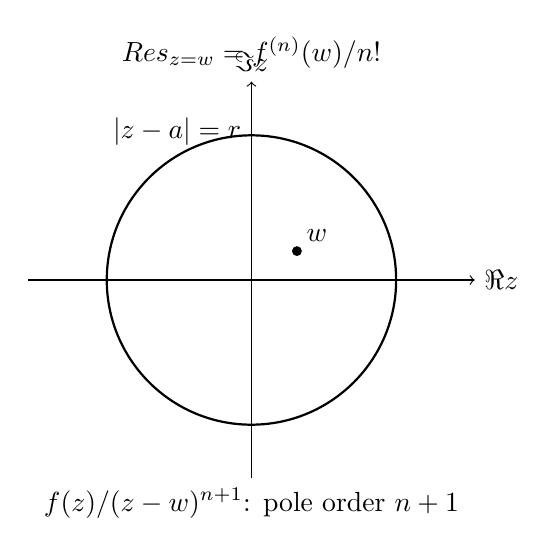
\begin{tikzpicture}[scale=1.05]
  \draw[->] (-2.7,0)--(2.7,0) node[right] {$\Re z$};
  \draw[->] (0,-2.4)--(0,2.4) node[above] {$\Im z$};
  \draw[thick,->] (0,0) circle (1.75);
  \fill (0.55,0.35) circle (1.7pt) node[above right] {$w$};
  \node at (-0.9,1.8) {$|z-a|=r$};
  \node at (0,-2.7) {$f(z)/(z-w)^{n+1}$: pole order $n+1$};
  \node at (0,2.75) {$\operatorname{Res}_{z=w}=f^{(n)}(w)/n!$};
\end{tikzpicture}
\caption{The integrand $f(z)/(z-w)^{n+1}$ has a single higher-order pole at $w$ inside the contour. Its residue is $f^{(n)}(w)/n!$, which is exactly the coefficient extracted by Cauchy's derivative formula.}
\label{fig:cp-iv-0139-higher-order-pole-cauchy}
\end{figure}


\begin{solution}
Let $g(z)=\dfrac{f(z)}{(z-w)^{n+1}}$. Then $g$ is meromorphic on $|z-a|\le r$ with a single pole of order $n+1$ at $z=w$.
Hence
\[
\operatorname{Res}(g;w)=\frac{1}{n!}\,f^{(n)}(w).
\]
Applying the residue theorem to the circle $|z-a|=r$ gives
\[
\int_{|z-a|=r}\frac{f(z)}{(z-w)^{n+1}}\,dz
= 2\pi i\,\operatorname{Res}(g;w)
= 2\pi i\,\frac{f^{(n)}(w)}{n!},
\]
which rearranges to the stated formula. For $n=0$ this is the usual Cauchy integral formula.

\medskip
\end{solution}

\section{Global Complex Analysis}

\par\medskip\noindent\textbf{Related material.}\quad Volume IV, Chapters \texttt{IV/12--IV/18}.

\begin{problem}[CP-IV-0004]
\label{prob:cp-iv-0004}
\par\noindent\textbullet\quad \textbf{(c)}\;
	Consider instead the branch
	\[
	f(z) \;=\; (r_{1}r_{2})^{1/2} \, e^{\,i(\theta_{1}+\theta_{2})/2},
	\qquad -\tfrac{3\pi}{2}<\theta_{1}\le \tfrac{\pi}{2},\quad
	-\tfrac{\pi}{2}<\theta_{2}\le \tfrac{3\pi}{2}.
	\]
	State the values of \((\theta_{1}+\theta_{2})/2\) on either side of the imaginary axis,
	and hence compute \(f(\pm0+iy)\) in terms of \(y\) for \(y\in\mathbb{R}\).
	Deduce that the branch cut is along the imaginary axis
	from \(z=-i\infty\) to \(z=-i\) and from \(z=i\) to \(z=i\infty\).
	Compute \(f(x)\) in terms of \(x\) for \(x\in\mathbb{R}\).
	Show that
	\[
	f(z)\sim
	\begin{cases}
		z,  & \text{as } |z|\to\infty \text{ with } \Re(z)>0,\\[2pt]
		-z,  & \text{as } |z|\to\infty \text{ with } \Re(z)<0.
	\end{cases}
	\]
	Sketch the images of the half-planes \(\Re(z)>0\) and \(\Re(z)<0\) under the map \(\zeta=f(z)\).

	\bigskip\hrule\bigskip
\end{problem}

% Designed Companion Part IV figure
% Intended for \input{...} beside the matching canonical problem.
\begin{figure}[ht]
\centering
\begin{tikzpicture}[scale=1.05]
  \draw[->] (-3.2,0)--(3.2,0) node[right] {$\Re z$};
  \draw[->] (0,-3.2)--(0,3.2) node[above] {$\Im z$};
  \fill (0,1) circle (1.5pt) node[right] {$i$};
  \fill (0,-1) circle (1.5pt) node[right] {$-i$};
  \draw[very thick] (0,1)--(0,3.0);
  \draw[very thick] (0,-1)--(0,-3.0);
  \node[right] at (0.15,2.25) {branch cut};
  \node[right] at (0.15,-2.25) {branch cut};
  \node at (1.85,1.2) {$f(z)\sim z$};
  \node at (-1.85,-1.2) {$f(z)\sim -z$};
  \node at (1.65,-2.55) {$\Re z>0$};
  \node at (-1.65,2.55) {$\Re z<0$};
\end{tikzpicture}
\caption{Branch points at $z=\pm i$ and the branch cuts running outward along the imaginary axis. The two half-planes carry the asymptotic signs $f(z)\sim z$ and $f(z)\sim -z$.}
\label{fig:cp-iv-0004-exterior-imaginary-branch-cuts}
\end{figure}


\begin{solution}
Write
\[
z-i=r_1e^{i\theta_1},
\qquad
z+i=r_2e^{i\theta_2}.
\]
The chosen ranges make the ray \(i[1,\infty)\) a cut for \(\theta_1\) and the ray \(-i[1,\infty)\) a cut for \(\theta_2\).

For \(y>1\), approaching the imaginary axis from the right gives
\[
\frac{\theta_1+\theta_2}{2}=\frac{\pi}{2},
\]
whereas approaching from the left gives \(-\pi/2\). Hence
\[
f(+0+iy)=i\sqrt{y^2-1},
\qquad
f(-0+iy)=-i\sqrt{y^2-1}.
\]
For \(y<-1\),
\[
f(+0+iy)=-i\sqrt{y^2-1},
\qquad
f(-0+iy)=i\sqrt{y^2-1}.
\]
For \(|y|<1\), no branch jump occurs and
\[
f(\pm0+iy)=\sqrt{1-y^2}.
\]
Thus the branch cuts are exactly
\[
i[1,\infty)
\quad\text{and}\quad
-i[1,\infty).
\]

For \(x\in\mathbb R\),
\[
f(x)=\sqrt{x^2+1}>0.
\]
As \(|z|\to\infty\),
\[
f(z)^2=z^2+1=z^2\left(1+\frac1{z^2}\right),
\]
so the chosen branch satisfies
\[
f(z)\sim z
\quad(\Re z>0),
\qquad
f(z)\sim -z
\quad(\Re z<0).
\]

Each half-plane is mapped conformally onto the slit right half-plane
\[
\{w:\Re w>0\}\setminus(0,1],
\]
with the two half-planes providing the two inverse branches of
\[
z^2=w^2-1.
\]
The middle segment \(-i<z<i\) maps to the slit \((0,1]\), while the two outer imaginary rays map to the positive and negative imaginary boundary rays.
\end{solution}


\begin{problem}[CP-IV-0007]
\label{prob:cp-iv-0007}
Temperature in a right half–plane with a removed disk

The domain $D$ consists of the right-hand half plane $x>0$ with the circle $|z-a|=b$, $0<b<a$, and its interior removed.
	Find the temperature $u(x,y)$ in steady heat flow if $u=0$ on the $y$ axis, $u=1$ on $|z-a|=b$, and $u\to0$ at infinity.

	\medskip
	\noindent\textit{Hint:} Show that the mapping $\displaystyle \zeta=\frac{z-\alpha}{z+\alpha}$, with $\alpha$ real and positive,
	takes $D$ onto an annular region with the imaginary axis mapping to $|\zeta|=1$ and show that, if $\alpha^{2}=a^{2}-b^{2}$, then the image of $D$ is a concentric circular annulus.

	\bigskip\hrule\bigskip

	Consider the real-parameter Möbius map
	\[
	\zeta=\zeta(z)=\frac{z-\alpha}{z+\alpha}, \qquad \alpha>0.
	\]

	For $z=iy$ we have
	\[
	\left|\frac{iy-\alpha}{iy+\alpha}\right|=1 \quad\text{(numerator and denominator are conjugates),}
	\]
	so the $y$–axis maps to the unit circle $|\zeta|=1$.

	\paragraph{Image of the circle $\boldsymbol{|z-a|=b}$.}
	Write $z=a+be^{i\theta}$ and compute
	\[
	|\zeta|^{2}
	=\frac{|a-\alpha+be^{i\theta}|^{2}}{|a+\alpha+be^{i\theta}|^{2}}
	=\frac{A+B\cos\theta}{C+D\cos\theta},
	\]
	where
	\[
	A=(a-\alpha)^{2}+b^{2}, \qquad B=2b(a-\alpha), \qquad
	C=(a+\alpha)^{2}+b^{2}, \qquad D=2b(a+\alpha).
	\]
	For $|\zeta|$ to be constant on the circle (i.e. the image is a circle \emph{centered at the origin}),
	the $\cos\theta$–dependence must drop out:
	\[
	\frac{A+B\cos\theta}{\,C+D\cos\theta\,}\equiv\frac{A}{C}
	\quad\Longleftrightarrow\quad AD=BC.
	\]
	We now verify that
	\[
	AD-BC
	=2b\Big[(a+\alpha)((a-\alpha)^{2}+b^{2})-(a-\alpha)((a+\alpha)^{2}+b^{2})\Big]
	=4b\alpha\,(\alpha^{2}+b^{2}-a^{2}).
	\]
	Thus $AD=BC$ is equivalent to
	\[
	\boxed{\ \alpha^{2}=a^{2}-b^{2}\ }.
	\]
	With this choice (note $a>b>0\Rightarrow \alpha>0$), the ratio becomes \emph{constant}:
	\[
	|\zeta|^{2}=\frac{A}{C}
	=\frac{(a-\alpha)^{2}+b^{2}}{(a+\alpha)^{2}+b^{2}}
	=\frac{2a(a-\alpha)}{2a(a+\alpha)}
	=\frac{a-\alpha}{a+\alpha}.
	\]
	Hence the circle $|z-a|=b$ maps to the circle $|\zeta|=\rho$ with
	\[
	\boxed{\ \rho=\sqrt{\frac{a-\alpha}{a+\alpha}}\in(0,1). \ }
	\]

	Therefore, for $\alpha=\sqrt{a^{2}-b^{2}}$, the map $z\mapsto\zeta$ sends the domain $D$
	(right half–plane with the closed disk $\{|z-a|\le b\}$ removed) onto the concentric circular \emph{annulus}
	\[
	\mathcal A=\{\ \rho<|\zeta|<1\ \}.
	\]
	The boundary pieces correspond as follows:
	\[
	\{x=0\}\ \longmapsto\ |\zeta|=1,
	\qquad
	\{|z-a|=b\}\ \longmapsto\ |\zeta|=\rho.
	\]

	\bigskip\hrule\bigskip

	Let $U(\zeta)$ denote the temperature in the $\zeta$–plane. Harmonicity is preserved by conformal maps, so
	$U$ is harmonic on $\mathcal A$ and the boundary data become
	\[
	U=0 \ \ \text{on}\ \ |\zeta|=1,
	\qquad
	U=1 \ \ \text{on}\ \ |\zeta|=\rho.
	\]
	By rotational symmetry, $U$ depends only on $r=|\zeta|$. The general radial harmonic function on an annulus is
	$A\log r + B$. Imposing the boundary values gives
	\[
	U(r)=\frac{\log(1/r)}{\log(1/\rho)}
	=\frac{-\log r}{-\log \rho}
	=\frac{\log r}{\log \rho}
	\quad\text{for}\quad \rho<r<1.
	\]
	(Any of the three displayed forms is correct; we will use the first one momentarily.)

	\bigskip\hrule\bigskip

	The physical temperature is $u(z)=U(\zeta(z))$ with $r=|\zeta(z)|=\left|\frac{z-\alpha}{z+\alpha}\right|$.
	Hence
	\[
	u(z)
	=U\!\left(\left|\frac{z-\alpha}{z+\alpha}\right|\right)
	=\frac{\displaystyle \log\!\left(\frac{1}{\left|\frac{z-\alpha}{z+\alpha}\right|}\right)}
	{\displaystyle \log\!\left(\frac{1}{\rho}\right)}
	=\frac{\displaystyle \log\left|\frac{z+\alpha}{z-\alpha}\right|}
	{\displaystyle \log\!\left(\frac{1}{\rho}\right)}.
	\]
	Since $\displaystyle \rho=\sqrt{\frac{a-\alpha}{a+\alpha}}$ we have
	\[
	\log\!\left(\frac{1}{\rho}\right)
	=\frac{1}{2}\,\log\!\left(\frac{a+\alpha}{a-\alpha}\right).
	\]
	Therefore a convenient explicit form is
	\[
	\boxed{\quad
		u(z)
		=\frac{2\,\log\!\left|\dfrac{z+\alpha}{z-\alpha}\right|}
		{\log\!\left(\dfrac{a+\alpha}{a-\alpha}\right)},
		\qquad
		\alpha=\sqrt{a^{2}-b^{2}}.
		\quad}
	\]

	\bigskip

		\par\noindent\textbullet\quad \textbf{On the $y$--axis $x=0$:} for $z=iy$ we have $\left|\dfrac{z-\alpha}{z+\alpha}\right|=1$,
		so the numerator $\log\left|\dfrac{z+\alpha}{z-\alpha}\right|=0$ and hence $u=0$.
		\par\noindent\textbullet\quad \textbf{On the circle $|z-a|=b$:} by construction $|\zeta|=\rho$, i.e.
		$\left|\dfrac{z-\alpha}{z+\alpha}\right|=\rho$, so
		$\log\left|\dfrac{z+\alpha}{z-\alpha}\right|=\log\!\left(\dfrac{1}{\rho}\right)$
		and the fraction evaluates to $u=1$.
		\par\noindent\textbullet\quad \textbf{At infinity:} as $|z|\to\infty$, $\left|\dfrac{z+\alpha}{z-\alpha}\right|\to 1$,
		so the numerator $\to 0$ and $u(z)\to 0$.

	\bigskip\hrule\bigskip

	With $\alpha=\sqrt{a^{2}-b^{2}}$ and $\displaystyle \rho=\sqrt{\frac{a-\alpha}{a+\alpha}}$,
	the Möbius map $\displaystyle \zeta=\frac{z-\alpha}{z+\alpha}$ carries
	$D$ onto the annulus $\{\rho<|\zeta|<1\}$.
	The unique harmonic function with $U=1$ on $|\zeta|=\rho$ and $U=0$ on $|\zeta|=1$
	is $U(r)=\log(1/r)/\log(1/\rho)$, and hence
	\[
	u(z)=\frac{2\,\log\!\left|\dfrac{z+\alpha}{z-\alpha}\right|}
	{\log\!\left(\dfrac{a+\alpha}{a-\alpha}\right)}.
	\]
	This $u$ satisfies all the prescribed boundary conditions and $u(z)\to 0$ as $|z|\to\infty$.

\textbf{Background:} entire, odd; period $2\pi i$. \quad
\textbf{Zeros:} $z=i\pi k$; \textbf{poles:} none.\\
\textbf{Decomposition: } $w=u+iv=\sinh x\cos y + i\,\cosh x\sin y$.\\
\textbf{Vertical lines } $x=\text{const}$: $\left(\frac{u}{\sinh x}\right)^2+\left(\frac{v}{\cosh x}\right)^2=1$ (ellipses, foci $\pm i$).\\
\textbf{Horizontal lines } $y=\text{const}$: $\left(\frac{u}{\cos y}\right)^2-\left(\frac{v}{\sin y}\right)^2=-1$ (hyperbolas, foci $\pm i$).\\
\textbf{Strip mapping:}
\[
\boxed{\,\sinh:\ \{|\Im z|<\tfrac{\pi}{2}\}\ \xrightarrow{\ 1\text{--}1\ }\ \mathbb C\setminus i\big((-\infty,-1]\cup[1,\infty)\big)\,}
\]
Boundaries $y=\pm\frac{\pi}{2}$ map to imaginary rays $\pm i[1,\infty)$.

\bigskip\hrule\bigskip

\textbf{Background:} entire, even; period $2\pi i$. \quad
\textbf{Zeros:} $z=i\pi(k+\frac12)$; \textbf{poles:} none.\\
\textbf{Decomposition: } $w=u+iv=\cosh x\cos y + i\,\sinh x\sin y$.\\
\textbf{Vertical lines } $x=\text{const}$: $\left(\frac{u}{\cosh x}\right)^2+\left(\frac{v}{\sinh x}\right)^2=1$ (ellipses, foci $\pm1$).\\
\textbf{Horizontal lines } $y=\text{const}$: $\left(\frac{u}{\cos y}\right)^2-\left(\frac{v}{\sin y}\right)^2=1$ (hyperbolas, foci $\pm1$).\\
\textbf{Strip mapping:}
\[
\boxed{\,\cosh:\ \{|\Im z|<\pi\}\ \xrightarrow{\ 2\text{--}1\ }\ \mathbb C\setminus\big((-\infty,-1]\cup[1,\infty)\big)\,}
\]
On the half-strip $0<|\Im z|<\pi$, the map is 1--1 onto the slit plane.

\bigskip\hrule\bigskip

\textbf{Background:} meromorphic, odd; period $i\pi$. \quad
\textbf{Zeros:} $z=i\pi k$; \textbf{poles:} $z=i\pi(k+\tfrac12)$.\\
\textbf{Strip $\to$ disk:}
\[
\boxed{\,\tanh:\ \{|\Im z|<\tfrac{\pi}{2}\}\ \xrightarrow{\ 1\text{--}1\ }\ \mathbb D\,}
\]
Real line maps to $(-1,1)$; as $|\Im z|\to\pi/2$, $|\tanh z|\to1$.

\bigskip\hrule\bigskip

\textbf{Background:} meromorphic, odd; period $i\pi$. \quad
\textbf{Zeros:} $z=i\pi(k+\tfrac12)$; \textbf{poles:} $z=i\pi k$.\\
\textbf{Strip $\to$ exterior disk:}
\[
\boxed{\,\coth:\ \{|\Im z|<\tfrac{\pi}{2}\}\setminus\{0\}\ \xrightarrow{\ 1\text{--}1\ }\ \{\,|w|>1\,\}\,}
\]
Real line maps to $(-\infty,-1)\cup(1,\infty)$; $|\Im z|\to\pi/2$ gives $|w|\to1^+$.

Throughout, write $z=x+iy$, $x,y\in\mathbb R$, and $w=u+iv$ for the image.
Recall the basic identities
\[
\cosh z=\frac{e^{z}+e^{-z}}{2},\qquad
\sinh z=\frac{e^{z}-e^{-z}}{2},\qquad
\tanh z=\frac{\sinh z}{\cosh z},\qquad
\coth z=\frac{\cosh z}{\sinh z}.
\]
We use the principal branch of the logarithm $\log$ on $\mathbb C\setminus(-\infty,0]$, and principal square roots $\sqrt{\cdot}$ with branch cut on $(-\infty,0]$ unless stated otherwise.

\bigskip\hrule\bigskip

 \mbox{}\\[2pt]
$\sinh$ is an \emph{entire}, \emph{odd} function, with imaginary-periodicity:
\[
\sinh(-z)=-\sinh z,\qquad \sinh(z+2\pi i)=\sinh z.
\]
Zeros occur at $z_k=i\pi k$ for $k\in\mathbb Z$ (all simple). No poles.

\medskip

 \mbox{}\\[2pt]
With $z=x+iy$,
\[
\sinh z=\sinh x\cos y\ +\ i\,\cosh x\sin y \quad\Rightarrow\quad
u=\sinh x\cos y,\ \ v=\cosh x\sin y.
\]
From this, one obtains orthogonal families of confocal conics:
\begin{align*}
	x=\text{const}&:\quad \left(\frac{u}{\sinh x}\right)^{2}+\left(\frac{v}{\cosh x}\right)^{2}=1
	&&\text{(ellipses, foci at $\pm i$)},\\[2pt]
	y=\text{const}&:\quad \left(\frac{u}{\cos y}\right)^{2}-\left(\frac{v}{\sin y}\right)^{2}=-1
	&&\text{(hyperbolas, foci at $\pm i$)}.
\end{align*}
Real and imaginary axes map as:
\[
y=0:\ w=\sinh x\in\mathbb R\ \text{(onto $\mathbb R$)},\qquad
x=0:\ w=i\sin y\ \text{(onto the segment $i[-1,1]$)}.
\]

\medskip

 \mbox{}\\[2pt]
$\sinh'(z)=\cosh z$, and $\cosh z\neq 0$ on the strip $|\Im z|<\tfrac{\pi}{2}$; hence $\sinh$ is conformal there.

\medskip

 \mbox{}\\[2pt]
\[
\boxed{\
	\sinh:\ \{\,|\Im z|<\tfrac{\pi}{2}\,\}\ \xrightarrow[\ \text{biholomorphism}\ ]{}\
	\mathbb C\setminus i\big((-\infty,-1]\cup[1,\infty)\big)\ .
}\]
\emph{Explanation.} The boundary lines $y=\pm\frac{\pi}{2}$ map to the imaginary rays $\pm i[1,\infty)$
(via $v=\cosh x\,\sin y$ with $\sin(\pm\pi/2)=\pm1$ and $u=\sinh x\cos(\pm\pi/2)=0$), while the interior maps injectively since $\cosh z\neq0$ and periodicity in the imaginary direction has period $2\pi$, not $\pi$.

\medskip

 \mbox{}\\[2pt]
A principal inverse on the slit domain is
\[
\operatorname{arsinh} w=\log\!\big(w+\sqrt{w^{2}+1}\big),
\]
with branch cuts along $i(-\infty,-1]\cup i[1,\infty)$ so that $\Im(\operatorname{arsinh} w)\in(-\tfrac{\pi}{2},\tfrac{\pi}{2})$.

\medskip

 \mbox{}\\[2pt]
\[
\cosh^{2}z-\sinh^{2}z=1,\qquad
\sinh(z+\zeta)=\sinh z\,\cosh\zeta+\cosh z\,\sinh\zeta.
\]

\bigskip\hrule\bigskip

 \mbox{}\\[2pt]
$\cosh$ is \emph{entire}, \emph{even}, and $2\pi i$-periodic:
\[
\cosh(-z)=\cosh z,\qquad \cosh(z+2\pi i)=\cosh z.
\]
Zeros at $z=i\pi\big(k+\tfrac12\big)$, all simple. No poles.

\medskip

 \mbox{}\\[2pt]
With $z=x+iy$,
\[
\cosh z=\cosh x\cos y\ +\ i\,\sinh x\sin y \quad\Rightarrow\quad
u=\cosh x\cos y,\ \ v=\sinh x\sin y.
\]
Again one gets confocal conics:
\begin{align*}
	x=\text{const}&:\quad \left(\frac{u}{\cosh x}\right)^{2}+\left(\frac{v}{\sinh x}\right)^{2}=1
	&&\text{(ellipses, foci at $\pm1$)},\\[2pt]
	y=\text{const}&:\quad \left(\frac{u}{\cos y}\right)^{2}-\left(\frac{v}{\sin y}\right)^{2}=1
	&&\text{(hyperbolas, foci at $\pm1$)}.
\end{align*}
On the axes,
\[
y=0:\ w=\cosh x\in[1,\infty),\qquad
x=0:\ w=\cos y\in[-1,1].
\]

\medskip

 \mbox{}\\[2pt]
$\cosh'(z)=\sinh z$, which vanishes at $z=i\pi k$. Thus $\cosh$ fails to be injective across lines $y=k\pi$, but is injective on any strip avoiding these lines (e.g.\ $0<\Im z<\pi$).

\medskip

 \mbox{}\\[2pt]
\[
\boxed{\
	\cosh:\ \{\,0<\Im z<\pi\,\}\ \xrightarrow[\ \text{biholomorphism}\ ]{}\
	\mathbb C\setminus\big((-\infty,-1]\cup[1,\infty)\big)\ .
}\]
\emph{Explanation.} The midline $y=0$ maps to $[1,\infty)$; the top boundary $y=\pi$ maps to $(-\infty,-1]$; injectivity holds on $0<\Im z<\pi$ since there $\sinh z\neq0$.

\medskip

 \mbox{}\\[2pt]
\[
\operatorname{arcosh} w=\log\!\Big(w+\sqrt{w-1}\,\sqrt{w+1}\Big),
\]
with branch cuts along $(-\infty,-1]\cup[1,\infty)$ so that $\Re(\operatorname{arcosh} w)\ge0$ and $0<\Im(\operatorname{arcosh} w)<\pi$ on the principal sheet.

\medskip

 \mbox{}\\[2pt]
\[
\cosh(z+\zeta)=\cosh z\,\cosh\zeta+\sinh z\,\sinh\zeta,\qquad
\cosh z=1+2\sinh^{2}\!\frac{z}{2}.
\]

\bigskip\hrule\bigskip

 \mbox{}\\[2pt]
$\tanh$ is \emph{meromorphic}, \emph{odd}, and $i\pi$-periodic:
\[
\tanh(-z)=-\tanh z,\qquad \tanh(z+i\pi)=\tanh z.
\]
Zeros at $z=i\pi k$; poles (simple) at $z=i\pi\big(k+\tfrac12\big)$.

\medskip

 \mbox{}\\[2pt]
\[
\boxed{\
	\tanh:\ \{\,|\Im z|<\tfrac{\pi}{2}\,\}\ \xrightarrow[\ \text{biholomorphism}\ ]{}\ \mathbb D\ .
}\]
\emph{Boundary correspondence.} The real axis $y=0$ maps bijectively onto $(-1,1)$ (strictly increasing).
As $y\to\pm\frac{\pi}{2}$, $|\tanh(x+iy)|\to1$ uniformly in $x$; hence the horizontal boundaries map to $\partial\mathbb D$.

\medskip

 \mbox{}\\[2pt]
\[
\operatorname{artanh} w=\frac{1}{2}\log\!\left(\frac{1+w}{1-w}\right),
\qquad |w|<1,
\]
which maps $\mathbb D$ conformally onto $\{|\Im z|<\tfrac{\pi}{2}\}$.

\medskip

 \mbox{}\\[2pt]
\[
(\tanh z)'=\operatorname{sech}^{2}\!z,\qquad
\left|\tanh'(z)\right|=\frac{1}{|\cosh z|^{2}}
\]
and conjugating by a disk automorphism shows $\tanh$ is extremal for the disk-strip version of Schwarz--Pick.

\medskip

 \mbox{}\\[2pt]
Lines $x=\text{const}$ and $y=\text{const}$ in the strip map to orthogonal circle arcs inside $\mathbb D$ meeting $\partial\mathbb D$ orthogonally (images of preimages under the conformal equivalence with the half-plane followed by a Cayley map).

\bigskip\hrule\bigskip

 \mbox{}\\[2pt]
$\coth$ is \emph{meromorphic}, \emph{odd}, and $i\pi$-periodic:
\[
\coth(-z)=-\coth z,\qquad \coth(z+i\pi)=\coth z.
\]
Poles (simple) at $z=i\pi k$; zeros (simple) at $z=i\pi\big(k+\tfrac12\big)$.

\medskip

 \mbox{}\\[2pt]
\[
\boxed{\
	\coth:\ \{\,|\Im z|<\tfrac{\pi}{2}\,\}\setminus\{0\}\ \xrightarrow[\ \text{biholomorphism}\ ]{}\ \{\,|w|>1\,\}\ .
}\]
\emph{Boundary correspondence.} The real axis (excluding $0$) maps to the rays $(-\infty,-1)\cup(1,\infty)$.
As $y\to\pm\frac{\pi}{2}$, $|\coth(x+iy)|\to1^{+}$; thus horizontal boundaries map to the unit circle from the \emph{exterior} side.

\medskip

 \mbox{}\\[2pt]
\[
\operatorname{arcoth} w=\frac{1}{2}\log\!\left(\frac{w+1}{w-1}\right),\qquad |w|>1,
\]
with the standard logarithm branch so that $\Im(\operatorname{arcoth} w)\in(-\tfrac{\pi}{2},\tfrac{\pi}{2})$.

\medskip

 \mbox{}\\[2pt]
\[
\coth z=\tanh\!\left(z+\tfrac{i\pi}{2}\right),
\]
so the exterior-disk picture is just the disk picture shifted vertically by $i\pi/2$ and inverted via $w\mapsto 1/w$.

\bigskip\hrule\bigskip

 \mbox{}\\[2pt]
\[
\operatorname{arsinh} w=\log\!\big(w+\sqrt{w^{2}+1}\big),\qquad
\operatorname{arcosh} w=\log\!\big(w+\sqrt{w-1}\,\sqrt{w+1}\big),
\]
\[
\operatorname{artanh} w=\frac12\log\!\left(\frac{1+w}{1-w}\right),\qquad
\operatorname{arcoth} w=\frac12\log\!\left(\frac{w+1}{w-1}\right).
\]
Branch cuts are chosen to match the canonical target domains described above.

\medskip

 \mbox{}\\[2pt]
Using the Cayley map $C(\zeta)=\frac{1+\zeta}{1-\zeta}$ and its inverse $C^{-1}(w)=\frac{w-1}{w+1}$,
\[
\tanh z=\ C^{-1}\!\left(e^{2z}\right),\qquad
\coth z=\ C^{-1}\!\left(e^{2z}\right)^{-1},\qquad
\sinh z=\frac{e^{z}-e^{-z}}{2},\quad \cosh z=\frac{e^{z}+e^{-z}}{2}.
\]
Thus strip $\leftrightarrow$ disk/exterior-disk mappings for $\tanh$ and $\coth$ are just the exponential’s strip-to-sector equivalences composed with a Cayley map.

\medskip

 \mbox{}\\[2pt]
As $x\to\pm\infty$ with $y$ fixed, $\sinh z\sim \frac12 e^{x}e^{iy}$ and $\cosh z\sim \frac12 e^{x}e^{iy}$; hence horizontal lines map to asymptotically radial curves. For $\tanh$ and $\coth$, $|\tanh(x+iy)|\to 1$ and $|\coth(x+iy)|\to 1$ exponentially in $|x|$ (uniform in $y$ within the strip height).

\medskip

 \mbox{}\\[2pt]
$\sinh'(z)=\cosh z$ vanishes along $y=\frac{\pi}{2}+\pi\mathbb Z$; $\cosh'(z)=\sinh z$ vanishes along $y=\pi\mathbb Z$.
Therefore, the natural injectivity strips are $|\Im z|<\tfrac{\pi}{2}$ for $\sinh$ and $0<\Im z<\pi$ for $\cosh$.
For $\tanh$ and $\coth$, poles on the horizontal boundaries determine the natural strip height $\pi$.

\bigskip\hrule\bigskip

\[
\boxed{\
	\sinh:\ \{\,|\Im z|<\tfrac{\pi}{2}\,\}\ \longrightarrow\
	\mathbb C\setminus i\big((-\infty,-1]\cup[1,\infty)\big)\ \ \text{(biholomorphism)}\ .
}\]
\[
\boxed{\
	\cosh:\ \{\,0<\Im z<\pi\,\}\ \longrightarrow\
	\mathbb C\setminus\big((-\infty,-1]\cup[1,\infty)\big)\ \ \text{(biholomorphism)}\ .
}\]
\[
\boxed{\
	\tanh:\ \{\,|\Im z|<\tfrac{\pi}{2}\,\}\ \longrightarrow\ \mathbb D\ \ \text{(biholomorphism)}\ .
}\]
\[
\boxed{\
	\coth:\ \{\,|\Im z|<\tfrac{\pi}{2}\,\}\setminus\{0\}\ \longrightarrow\ \{\,|w|>1\,\}\ \ \text{(biholomorphism)}\ .
}\]

\medskip

If $\sinh z_{1}=\sinh z_{2}$ then $e^{z_{1}}-e^{-z_{1}}=e^{z_{2}}-e^{-z_{2}}$.
Rearranging gives $\{e^{z_{1}},e^{-z_{1}}\}=\{e^{z_{2}},e^{-z_{2}}\}$.
Taking logs in the horizontal strip $|\Im z|<\pi/2$ (where the exponential is injective modulo $2\pi i$) forces $z_{1}=z_{2}$.

Set $z=x\pm i\pi/2$. Then $\sinh z=\sinh x\cdot 0 \ \pm i\,\cosh x$, so the boundaries map to $\pm i[1,\infty)$; the interior cannot reach those rays by the open mapping theorem and the maximum modulus principle applied to $1/(\sinh z\mp i)$.

  apply to $\cosh$ (use $\sinh$ zeros to avoid critical lines) and to $\tanh,\coth$ using the representation via exponentials and the Cayley transform.

We use principal branches of $\log$ and $\sqrt{\cdot}$ with branch cut $(-\infty,0]$ unless stated otherwise.
For each inverse, the principal domain is obtained by slitting the $w$–plane along the images of the multiple values.

\bigskip\hrule\bigskip

 \mbox{}\\[2pt]
\BoxEq{ \arcsin w = -\,i\,\log\!\Big(i\,w+\sqrt{\,1-w^{2}\,}\Big) }

 \mbox{}\\[2pt]
Branch points at $w=\pm1$; principal cuts along $(-\infty,-1]\cup[1,\infty)$.

 \mbox{}\\[2pt]
\BoxEq{ \arcsin:\ \mathbb C\setminus\big((-\infty,-1]\cup[1,\infty)\big)\ \longrightarrow\ \{\,|\Re z|<\tfrac{\pi}{2}\,\} }
For $w\in(-1,1)$, $\arcsin w\in(-\tfrac{\pi}{2},\tfrac{\pi}{2})\subset\mathbb R$.
For $w>1$,
$\arcsin w=\tfrac{\pi}{2}-i\,\operatorname{arcosh} w$ (hence $\Re=\tfrac{\pi}{2}$);
for $w<-1$,
$\arcsin w=-\tfrac{\pi}{2}+i\,\operatorname{arcosh}(-w)$ (hence $\Re=-\tfrac{\pi}{2}$).

 \mbox{}\\[2pt]
Approaching the cuts $[1,\infty)$ or $(-\infty,-1]$ forces $\Re \arcsin w\to \pm\tfrac{\pi}{2}$ and $|\Im \arcsin w|\to\infty$.
The real axis segment $(-1,1)$ maps to the real segment $(-\tfrac{\pi}{2},\tfrac{\pi}{2})$.

\bigskip\hrule\bigskip

 \mbox{}\\[2pt]
\BoxEq{ \arccos w = \frac{\pi}{2}-\arcsin w }
\BoxEq{ \arccos w = \frac{1}{i}\,\log\!\Big(w+\sqrt{w-1}\,\sqrt{w+1}\Big) }

 \mbox{}\\[2pt]
Same as $\arcsin$: branch points $\pm1$; cuts $(-\infty,-1]\cup[1,\infty)$.

 \mbox{}\\[2pt]
\BoxEq{ \arccos:\ \mathbb C\setminus\big((-\infty,-1]\cup[1,\infty)\big)\ \longrightarrow\ \{\,0<\Re z<\pi\,\} }
For $w\in(-1,1)$, $\arccos w\in(0,\pi)\subset\mathbb R$.
For $w>1$, $\arccos w=i\,\operatorname{arcosh} w$ (so $\Re=0$);
for $w<-1$, $\arccos w=\pi - i\,\operatorname{arcosh}(-w)$ (so $\Re=\pi$).

 \mbox{}\\[2pt]
The two slits map to the vertical strip boundaries $\Re z=0$ and $\Re z=\pi$.
The central interval $(-1,1)$ maps to the real segment $(0,\pi)$.

\bigskip\hrule\bigskip

 \mbox{}\\[2pt]
\BoxEq{ \arctan w = \frac{1}{2i}\,\log\!\left(\frac{1+i\,w}{\,1-i\,w\,}\right) }

 \mbox{}\\[2pt]
Branch points at $w=\pm i$; principal cuts $i(-\infty,-1]\cup i[1,\infty)$ along the imaginary axis beyond $\pm i$.

 \mbox{}\\[2pt]
\BoxEq{ \arctan:\ \mathbb C\setminus i\big((-\infty,-1]\cup[1,\infty)\big)\ \longrightarrow\ \{\,|\Re z|<\tfrac{\pi}{2}\,\} }
On $\mathbb R$, $\arctan \mathbb R=(-\tfrac{\pi}{2},\tfrac{\pi}{2})$.
Approaching $w=\pm i\,t$ ($t\ge1$) drives $\Re \arctan w\to \pm\tfrac{\pi}{2}$ and $|\Im|\to\infty$.

 \mbox{}\\[2pt]
$\arctan(-w)=-\arctan w$; conjugation across the real axis preserves values away from cuts.

\bigskip\hrule\bigskip

 \mbox{}\\[2pt]
\BoxEq{ \arccot w = \frac{1}{2i}\,\log\!\left(\frac{w+i}{\,w-i\,}\right) }
\BoxEq{ \arccot w = \frac{\pi}{2}-\arctan w }

 \mbox{}\\[2pt]
As for $\arctan$: branch points at $w=\pm i$; cuts $i(-\infty,-1]\cup i[1,\infty)$.

 \mbox{}\\[2pt]
\BoxEq{ \arccot:\ \mathbb C\setminus i\big((-\infty,-1]\cup[1,\infty)\big)\ \longrightarrow\ \{\,0<\Re z<\pi\,\} }
On $\mathbb R$, $\arccot \mathbb R=(0,\pi)$.
Approaching the cuts pins the image to $\Re z=0$ or $\Re z=\pi$ with $|\Im|\to\infty$.

\bigskip\hrule\bigskip

\[
\arcsin w + \arccos w = \frac{\pi}{2},\qquad
\arctan w + \arccot w = \frac{\pi}{2}.
\]
\[
\arcsin w = -\,i\,\operatorname{arsinh}(i w),\qquad
\arccos w = \operatorname{arcosh} w \cdot \frac{1}{i}\ \ (\text{on }[1,\infty)).
\]
\[
\arctan w = \frac{1}{2i}\big(\log(1+i w)-\log(1-i w)\big),\quad
\arccot w = \frac{1}{2i}\big(\log(w+i)-\log(w-i)\big).
\]

\medskip

	\par\noindent\textbullet\quad $\arcsin$: real on $(-1,1)$; the cuts map to $\Re z=\pm\tfrac{\pi}{2}$.
	\par\noindent\textbullet\quad $\arccos$: real on $(-1,1)$; the cuts map to $\Re z=0,\ \pi$.
	\par\noindent\textbullet\quad $\arctan$: real on $\mathbb R$; the imaginary-axis cuts beyond $\pm i$ map to $\Re z=\pm\tfrac{\pi}{2}$.
	\par\noindent\textbullet\quad $\arccot$: real on $\mathbb R$; the same cuts map to $\Re z=0,\ \pi$.

	\par\noindent\textbullet\quad \textbf{Cayley (disk $\leftrightarrow$ right half-plane).}\\[2pt]
	\[
	\boxed{\,w=\frac{1+z}{1-z}\,}\qquad\text{inverse:}\quad z=\frac{w-1}{w+1}.
	\]

	\par\noindent\textbullet\quad \textbf{Half-plane $\to$ half-plane (three-point normalization).}\\[2pt]
	\[
	\boxed{\,w=\frac{(z-a)(c-b)}{(z-b)(c-a)}\,}.
	\]

	\par\noindent\textbullet\quad \textbf{Disk automorphisms.}\\[2pt]
	\[
	\boxed{\,\phi_{a,\theta}(z)=e^{i\theta}\frac{z-a}{1-\bar a z}\,},\qquad |a|<1.
	\]

	\par\noindent\textbullet\quad \textbf{Strip $|\Im z|<h/2$ $\to$ right half-plane.}\\[2pt]
	\[
	\boxed{\,w=\exp\!\left(\frac{\pi z}{h}\right)\,}.
	\]

	\par\noindent\textbullet\quad \textbf{Strip $|\Im z|<h/2$ $\to$ unit disk.}\\[2pt]
	\[
	\boxed{\,\zeta=\frac{e^{\pi z/h}-1}{\,e^{\pi z/h}+1\,}\,}.
	\]

	\par\noindent\textbullet\quad \textbf{Strip $\to$ strip (height scaling).}\\[2pt]
	\[
	\boxed{\,z\mapsto \frac{h_2}{h_1}\,z\,}.
	\]

	\par\noindent\textbullet\quad \textbf{Band $a<\Im z<b$ $\to$ centered strip.}\\[2pt]
	\[
	\boxed{\,z\mapsto \frac{\pi}{b-a}\!\left(z-i\frac{a+b}{2}\right)\,}.
	\]

	\par\noindent\textbullet\quad \textbf{Sector $\{0<\arg z<\alpha\}$ $\to$ upper half-plane.}\\[2pt]
	\[
	\boxed{\,w=z^{\pi/\alpha}\,}\ \ \text{(principal branch)}.
	\]

	\par\noindent\textbullet\quad \textbf{Wedge $\to$ disk.}\\[2pt]
	Compose item (8) with Cayley (item 1).

	\par\noindent\textbullet\quad \textbf{Upper half-plane $\to$ disk (prescribed triple).}\\[2pt]
	\[
	\boxed{\,\Phi(z)=\frac{(z-a)}{(z-\bar a)}\cdot \frac{(b-\bar a)}{(b-a)}\,}.
	\]

	\par\noindent\textbullet\quad \textbf{Annulus $r<|z|<1$ $\leftrightarrow$ strip.}\\[2pt]
	\[
	\boxed{\,w=\log z\,}\quad\text{maps to }\ \log r<\Re w<0.
	\]

	\par\noindent\textbullet\quad \textbf{Annulus $\to$ disk.}\\[2pt]
	Use $w=\log z$ then item (5).

	\par\noindent\textbullet\quad \textbf{Half-plane minus disk $\to$ annulus.}\\[2pt]
	\[
	\boxed{\,\zeta=\frac{z-\alpha}{z+\alpha}\,},\qquad \alpha^{2}=a^{2}-b^{2}.
	\]

	\par\noindent\textbullet\quad \textbf{Disk with off-center hole $\to$ annulus.}\\[2pt]
	Center via $\phi_a$ (item 3), then items (11)–(12).

	\par\noindent\textbullet\quad \textbf{Punctured plane $\leftrightarrow$ cylinder.}\\[2pt]
	\[
	\boxed{\,w=\log z\,}\quad(\text{period }2\pi i).
	\]

	\par\noindent\textbullet\quad \textbf{Strip $\to$ punctured plane.}\\[2pt]
	\[
	\boxed{\,z\mapsto e^{z}\,}.
	\]

	\par\noindent\textbullet\quad \textbf{Ray-slit plane $\mathbb C\setminus[0,\infty)$ $\to$ half-plane.}\\[2pt]
	\[
	\boxed{\,w=\sqrt{z}\,}\ \ \text{(choose branch)}.
	\]

	\par\noindent\textbullet\quad \textbf{Segment-slit plane $\mathbb C\setminus[a,b]$ $\to$ half-plane.}\\[2pt]
	\[
	\boxed{\,w=\sqrt{\frac{z-a}{\,z-b\,}}\,}.
	\]

	\par\noindent\textbullet\quad \textbf{Exterior of $[-1,1]$ $\leftrightarrow$ exterior unit circle (Joukowski).}\\[2pt]
	\[
	\boxed{\,w=z+\frac{1}{z}\,},\qquad
	z=\frac{w\pm\sqrt{w^{2}-4}}{2}.
	\]

	\par\noindent\textbullet\quad \textbf{Exterior of ellipse $\leftrightarrow$ exterior unit circle.}\\[2pt]
	\[
	\boxed{\,w=\tfrac12\!\left(c z+\frac{1}{c z}\right)\,}\quad(\text{$c$ from axes}).
	\]

	\par\noindent\textbullet\quad \textbf{Right half-plane $\to$ vertical strip.}\\[2pt]
	\[
	\boxed{\,z\mapsto \frac{1}{\pi}\log\frac{z-1}{\,z+1\,}\,}.
	\]

	\par\noindent\textbullet\quad \textbf{Upper half-plane $\to$ rectangle (SC/elliptic).}\\[2pt]
	\[
	\boxed{\,\zeta=\int^z \frac{dt}{\sqrt{(t-a)(t-b)(t-c)(t-d)}}\,}.
	\]

	\par\noindent\textbullet\quad \textbf{Rectangle $\to$ disk (Jacobi sn).}\\[2pt]
	\[
	\boxed{\,\zeta=\operatorname{sn}\!\left(\frac{K(k)}{L}\,z;\,k\right)\,}.
	\]

	\par\noindent\textbullet\quad \textbf{Half-disk $\leftrightarrow$ half-plane.}\\[2pt]
	Restriction of Cayley (item 1) and inverse.

	\par\noindent\textbullet\quad \textbf{Lens (intersection of two disks) $\to$ disk.}\\[2pt]
	Möbius normalizes the circles; then a power map; then Cayley.

	\par\noindent\textbullet\quad \textbf{Half-strip $\{x>0,\ 0<\Im z<h\}$ $\to$ half-disk.}\\[2pt]
	\[
	\boxed{\,\exp(\pi z/h)\,}\ \ \text{then power, then Cayley}.
	\]

	\par\noindent\textbullet\quad \textbf{Polygon $\to$ half-plane (Schwarz--Christoffel).}\\[2pt]
	\[
	\boxed{\,\Phi'(z)=C\prod_k (z-z_k)^{\alpha_k-1}\,},\qquad \sum\alpha_k=2.
	\]

	\par\noindent\textbullet\quad \textbf{Upper half-plane $\to$ slit half-plane.}\\[2pt]
	\[
	\boxed{\,w=z+\frac{1}{z}\,}\ \ \text{then a real Möbius adjustment}.
	\]

	\par\noindent\textbullet\quad \textbf{Disk $\to$ disk with boundary arc removed.}\\[2pt]
	Automorphism to put endpoints at $\pm1$, then boundary power $z^\lambda$.

	\par\noindent\textbullet\quad \textbf{Finite Blaschke product (disk $\to$ disk, degree $n$).}\\[2pt]
	\[
	\boxed{\,B(z)=e^{i\theta}\prod_{k=1}^n \frac{z-a_k}{\,1-\bar a_k z\,}\,}.
	\]

 \mbox{}\\[2pt]
\[
w=\frac{1+z}{\,1-z\,}
\quad\text{maps}\quad
\mathbb D=\{|z|<1\}\ \text{onto}\ \{\,\Re w>0\,\},
\qquad
z=\frac{w-1}{\,w+1\,}
\]
is the inverse.

\medskip

 \mbox{}\\[2pt]
Compute
\[
\Re\!\left(\frac{1+z}{\,1-z\,}\right)
=\frac{\,1-|z|^{2}\,}{\,|1-z|^{2}\,}.
\]
Thus $\Re w>0$ for $|z|<1$, and $\Re w=0$ for $|z|=1$ (except $z=1$, which maps to $w=\infty$).
Therefore
\[
|z|<1\ \Longleftrightarrow\ \Re w>0,
\qquad
|z|=1\ \Longleftrightarrow\ \Re w=0 .
\]

\medskip

 \mbox{}\\[2pt]
$z=0\mapsto w=1$,
\quad
$z\to1^{-}\mapsto w\to+\infty$,
\quad
and $\partial\mathbb D\setminus\{1\}$ maps to the line $\Re w=0$.\\[2pt]
Circles/lines orthogonal to $\partial\mathbb D$ map to \emph{vertical} lines in the $w$–plane.

\bigskip\hrule\bigskip

 \mbox{}\\[2pt]
Let $L$ be a line or circle, and choose three distinct points $a,b,c\in L$. Define
\[
\Phi(z)=\frac{(z-a)(c-b)}{(z-b)(c-a)}.
\]
Then $\Phi(L)\subset\mathbb R\cup\{\infty\}$, with
\[
\Phi(a)=0,\qquad \Phi(b)=\infty,\qquad \Phi(c)=1,
\]
and the two sides of $L$ map to the half-planes $\Im\Phi(z)\gtrless 0$.

\medskip

 \mbox{}\\[2pt]
Given half-planes $H_1,H_2$ with boundary arcs $L_1,L_2$,
pick ordered boundary triples $a,b,c\in L_1$ and $A,B,C\in L_2$ (same cyclic order).
Then
\[
T(z)=\frac{(z-a)(c-b)}{(z-b)(c-a)}\cdot\frac{(C-A)}{(C-B)}
\]
is a Möbius map sending $L_1\!\to L_2$ with
\[
a\mapsto A,\qquad b\mapsto B,\qquad c\mapsto C,
\]
and taking the chosen side of $H_1$ onto the chosen side of $H_2$.

\medskip

 \mbox{}\\[2pt]
To send $L$ to $\mathbb R$, use $\Phi$ above; then pre/postcompose with an \emph{affine real} map
\[
\xi\longmapsto \alpha\,\xi+\beta,\qquad \alpha>0,
\]
to obtain any target half-plane, e.g.\ $\Re w>0$ or $\Im w>0$.
\end{problem}

% Designed Companion Part IV figure
% Intended for \input{...} beside the matching canonical problem.
\begin{figure}[ht]
\centering
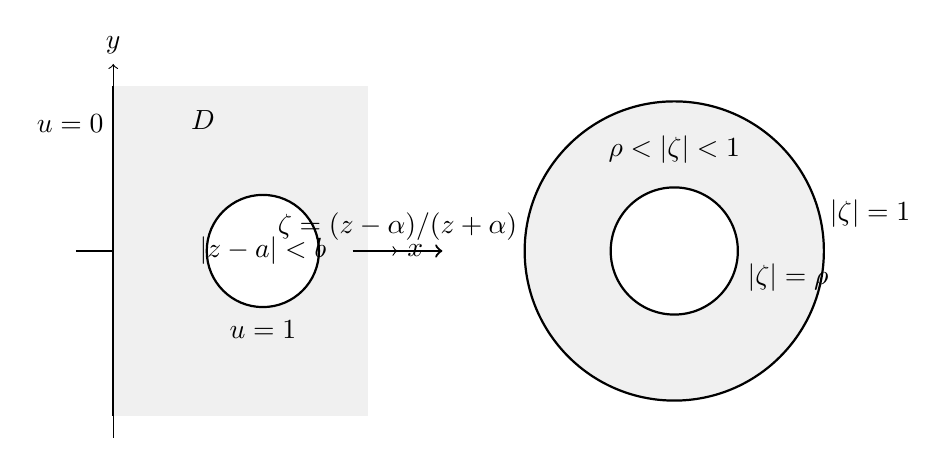
\begin{tikzpicture}[scale=0.95]
  \begin{scope}[xshift=-3.5cm]
    \draw[->] (-0.5,0)--(3.8,0) node[right] {$x$};
    \draw[->] (0,-2.5)--(0,2.5) node[above] {$y$};
    \fill[gray!12] (0,-2.2) rectangle (3.4,2.2);
    \fill[white] (2.0,0) circle (0.75);
    \draw[thick] (0,-2.2)--(0,2.2);
    \draw[thick] (2.0,0) circle (0.75);
    \node at (2.0,0) {$|z-a|<b$};
    \node at (1.2,1.75) {$D$};
    \node[left] at (0,1.7) {$u=0$};
    \node at (2.0,-1.05) {$u=1$};
  \end{scope}
  \draw[->,thick] (-0.3,0)--(0.9,0) node[midway,above] {$\zeta=(z-\alpha)/(z+\alpha)$};
  \begin{scope}[xshift=4.0cm]
    \fill[gray!12] (0,0) circle (2);
    \fill[white] (0,0) circle (0.85);
    \draw[thick] (0,0) circle (2);
    \draw[thick] (0,0) circle (0.85);
    \node at (0,1.35) {$\rho<|\zeta|<1$};
    \node[right] at (1.95,0.5) {$|\zeta|=1$};
    \node[right] at (0.85,-0.35) {$|\zeta|=\rho$};
  \end{scope}
\end{tikzpicture}
\caption{The Möbius map with $\alpha^2=a^2-b^2$ sends the right half-plane with the disk $|z-a|\le b$ removed to a concentric annulus. The $y$-axis becomes $|\zeta|=1$ and the circular obstacle becomes $|\zeta|=\rho$.}
\label{fig:cp-iv-0007-heat-domain-to-annulus}
\end{figure}


\begin{solution}
Set
\[
\alpha=\sqrt{a^2-b^2}>0
\]
and use
\[
\zeta=\frac{z-\alpha}{z+\alpha}.
\]
If \(z=iy\), numerator and denominator have equal modulus, so
\[
|\zeta|=1.
\]
Thus the imaginary axis maps to the unit circle.

For \(z=a+be^{i\theta}\),
\[
|\zeta|^2
=
\frac{(a-\alpha)^2+b^2+2b(a-\alpha)\cos\theta}
{(a+\alpha)^2+b^2+2b(a+\alpha)\cos\theta}.
\]
The condition \(\alpha^2=a^2-b^2\) makes this ratio independent of \(\theta\), and
\[
|\zeta|^2
=
\frac{a-\alpha}{a+\alpha}.
\]
Hence the circular boundary maps to
\[
|\zeta|=\rho,
\qquad
\rho=
\sqrt{\frac{a-\alpha}{a+\alpha}},
\]
and the physical domain maps to the annulus
\[
\rho<|\zeta|<1.
\]

The harmonic function on this annulus with values \(1\) on the inner circle and \(0\) on the outer circle is radial:
\[
U(\zeta)
=
\frac{\log(1/|\zeta|)}{\log(1/\rho)}.
\]
Therefore
\[
u(z)
=
\frac{\log\left|\frac{z+\alpha}{z-\alpha}\right|}
{\log(1/\rho)}.
\]
Since
\[
\log(1/\rho)
=
\frac12
\log\left(\frac{a+\alpha}{a-\alpha}\right),
\]
we obtain
\[
\boxed{
u(z)
=
\frac{
2\log\left|\frac{z+\alpha}{z-\alpha}\right|
}{
\log\left(\frac{a+\alpha}{a-\alpha}\right)
},
\qquad
\alpha=\sqrt{a^2-b^2}.
}
\]
On the imaginary axis the numerator is zero; on \(|z-a|=b\) it equals the denominator; and as \(|z|\to\infty\) it tends to zero. Thus all three prescribed conditions are satisfied.
\end{solution}


\begin{problem}[CP-IV-0008]
\label{prob:cp-iv-0008}
(Gaussian curvature formula and isolated zeros)

Let a minimal surface be given by Weierstrass data $(f,g)$ as in Problem 8:
	\[
	X(z)=\Re\int^z \Big(\tfrac12 f(1-g^2),\ \tfrac{i}{2}f(1+g^2),\ fg\Big)\,dz.
	\]

	\medskip
	\textbf{Step 1: induced metric.}
	In the parameter $z=u+iv$ the parametrization is conformal and one has
	\[
	ds^2=\lambda^2|dz|^2,\qquad
	\lambda=\frac{|f|(1+|g|^2)}{2},
	\]
	equivalently
	\[
	E=G=\lambda^2=\frac{|f|^2(1+|g|^2)^2}{4},\qquad F=0.
	\]

	\medskip
	\textbf{Step 2: Gauss map and stereographic projection.}
	For a minimal surface, the Gauss map $N:S\to S^2$ is conformal in conformal coordinates, and its stereographic
	coordinate is precisely $g$. The round metric on $S^2$ written in the stereographic coordinate $g$ is
	\[
	ds^2_{S^2}=\frac{4}{(1+|g|^2)^2}|dg|^2,
	\]
	so the pullback satisfies
	\[
	|N_u|^2+|N_v|^2=\frac{4}{(1+|g|^2)^2}\bigl(|g_u|^2+|g_v|^2\bigr).
	\]
	Since $g$ is holomorphic (meromorphic), $g_u=g'(z)$ and $g_v=i g'(z)$, hence
	\[
	|g_u|^2+|g_v|^2=2|g'(z)|^2,
	\]
	and therefore
	\[
	|N_u|^2+|N_v|^2=\frac{8|g'|^2}{(1+|g|^2)^2}.
	\]

	\medskip
	\textbf{Step 3: relate $K$ to $dN$ for minimal surfaces.}
	In an orthonormal basis of $T_pS$, the eigenvalues of $dN_p$ are $-k_1,-k_2$.
	For a minimal surface $k_2=-k_1$, so $K=k_1k_2=-k_1^2\le 0$ and
	\[
	\|dN\|^2=k_1^2+k_2^2=2k_1^2=-2K,
	\qquad\text{hence}\qquad
	K=-\frac12\|dN\|^2.
	\]
	In conformal coordinates, an orthonormal basis is $e_1=X_u/\lambda$, $e_2=X_v/\lambda$, so
	\[
	\|dN\|^2=\frac{|N_u|^2+|N_v|^2}{\lambda^2}.
	\]
	Thus
	\[
	K=-\frac12\frac{|N_u|^2+|N_v|^2}{\lambda^2}
	=-\frac12\frac{\frac{8|g'|^2}{(1+|g|^2)^2}}{\frac{|f|^2(1+|g|^2)^2}{4}}
	=-\frac{16|g'|^2}{|f|^2(1+|g|^2)^4}.
	\]
	Equivalently,
	\[
	K=-\left(\frac{4|g'|}{|f|(1+|g|^2)^2}\right)^2.
	\]

	\medskip
	\textbf{Zeros of $K$.}
	Assume the surface is regular (no branch points), so $f\neq 0$.
	Then $K(p)=0$ iff $g'(p)=0$.
	But $g'$ is holomorphic wherever $g$ is holomorphic, hence either $g'\equiv 0$ or its zeros are isolated.
	If $g'\equiv 0$, then $g$ is constant, the Gauss map is constant, and the surface is a plane, so $K\equiv 0$.
	Otherwise, the zeros of $g'$ (hence of $K$) are isolated.
\end{problem}

% Designed Companion Part IV figure
% Intended for \input{...} beside the matching canonical problem.
\begin{figure}[ht]
\centering
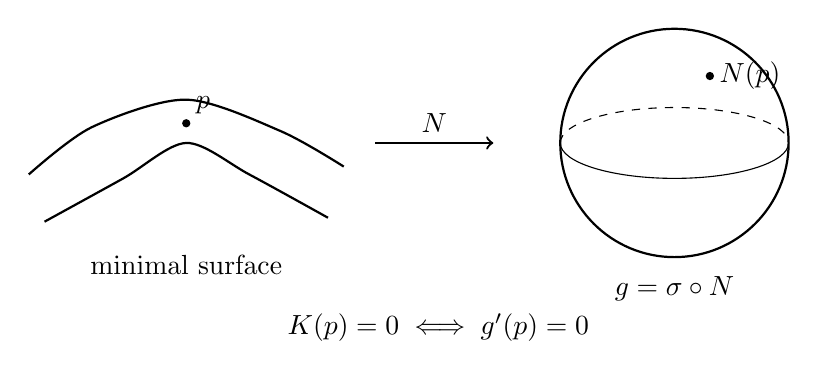
\begin{tikzpicture}[scale=1.0]
  \begin{scope}[xshift=-3.2cm]
    \draw[thick] plot[smooth] coordinates {(-2,-0.4) (-1.2,0.2) (0,0.55) (1.2,0.15) (2,-0.3)};
    \draw[thick] plot[smooth] coordinates {(-1.8,-1.0) (-0.8,-0.45) (0,0) (0.8,-0.4) (1.8,-0.95)};
    \fill (0,0.25) circle (1.5pt) node[above right] {$p$};
    \node at (0,-1.55) {minimal surface};
  \end{scope}
  \draw[->,thick] (-0.8,0)--(0.7,0) node[midway,above] {$N$};
  \begin{scope}[xshift=3.0cm]
    \draw[thick] (0,0) circle (1.45);
    \draw (-1.45,0) arc[start angle=180,end angle=360,x radius=1.45,y radius=0.45];
    \draw[dashed] (-1.45,0) arc[start angle=180,end angle=0,x radius=1.45,y radius=0.45];
    \fill (0.45,0.85) circle (1.5pt) node[right] {$N(p)$};
    \node at (0,-1.85) {$g=\sigma\circ N$};
  \end{scope}
  \node at (0,-2.35) {$K(p)=0\iff g'(p)=0$};
\end{tikzpicture}
\caption{For a regular minimal surface, $K=-16|g'|^2/(|f|^2(1+|g|^2)^4)$, so flat points are precisely critical points of the stereographic Gauss map $g$. Unless the surface is a plane, these critical points are isolated.}
\label{fig:cp-iv-0008-curvature-gauss-map}
\end{figure}


\begin{solution}
The Weierstrass metric is
\[
ds^2=\lambda^2|dz|^2,
\qquad
\lambda=\frac{|f|(1+|g|^2)}{2}.
\]
The stereographic metric on the sphere is
\[
ds_{S^2}^2
=
\frac{4|dg|^2}{(1+|g|^2)^2}.
\]
Since \(g\) is holomorphic,
\[
|g_u|^2+|g_v|^2=2|g'(z)|^2,
\]
and hence
\[
|N_u|^2+|N_v|^2
=
\frac{8|g'|^2}{(1+|g|^2)^2}.
\]

For a minimal surface the principal curvatures satisfy
\[
k_2=-k_1,
\]
so
\[
K=-k_1^2
\]
and
\[
\|dN\|^2=k_1^2+k_2^2=-2K.
\]
In conformal coordinates,
\[
\|dN\|^2
=
\frac{|N_u|^2+|N_v|^2}{\lambda^2}.
\]
Combining the formulas gives
\[
\boxed{
K
=
-\frac{16|g'|^2}
{|f|^2(1+|g|^2)^4}.
}
\]

At a regular point \(f\neq0\), therefore,
\[
K=0
\iff
g'=0.
\]
If \(g'\not\equiv0\), its zeros are isolated, so the flat points are isolated. If \(g'\equiv0\), then \(g\) is constant, the Gauss map is constant, and the surface is planar; in that case \(K\equiv0\).
\end{solution}


\begin{problem}[CP-IV-0016]
\label{prob:cp-iv-0016}
— Conformal mappings

\noindent
	(a)\; $D$ is the region exterior to the two circles $|z-1|=1$ and $|z+1|=1$.
	Find a conformal mapping from $D$ to the exterior of the unit circle.\\
	\emph{Hint:} First apply an inversion with respect to the origin $(z\mapsto 1/z)$,
	then rotate and scale so as to use the exponential function to get to a half plane,
	from where use Möbius.

	\medskip
	\noindent
	(b)\; Find a conformal map from the unit disc $|z|<1$ onto the strip $-\pi/2<\eta<\pi/2$,
	taking the origin to the origin, $1$ to $\xi=+\infty$, $-1$ to $\xi=-\infty$.
	(Thus, the upper half of the unit circle maps to $\eta=\pi/2$ and the lower half to $\eta=-\pi/2$.)

	\medskip
	\noindent
	(c)\; Find a conformal map of the quarter-disc $0<|z|<1,\ 0<\arg z<\pi/2$
	to the upper half-plane $\eta>0$, taking $0$ to $0$, $1$ to $1$, and $i$ to $\infty$.

	\bigskip\hrule\bigskip

		\setlength{\itemsep}{0.4em}
		\par\noindent\textbullet\quad \textbf{Invert.} Let $w=1/z$. Then the circles through $0$ become lines:
		\[
		|z-1|=1 \Rightarrow \Re w=\tfrac12,\qquad
		|z+1|=1 \Rightarrow \Re w=-\tfrac12.
		\]
		Hence $D$ maps to the vertical strip $S=\{-\tfrac12<\Re w<\tfrac12\}$.
		\par\noindent\textbullet\quad \textbf{Rotate/scale to a horizontal strip.} Put $s=i\pi w$.
		Then $|\Im s|<\pi/2$.
		\par\noindent\textbullet\quad \textbf{Exponential to a half-plane.} Let $u=e^{\,s}$.
		Then $|\Im s|<\pi/2 \;\Longrightarrow\; \Re u>0$.
		\par\noindent\textbullet\quad \textbf{Möbius to exterior unit disk.} Use

	\[
	\Phi(u)=\frac{u+1}{u-1},\qquad \operatorname{Re} u>0 \longmapsto |\zeta|>1.
	\]

	Therefore a concrete map is
	\[
	\boxed{\ \zeta=\Phi\!\big(e^{\,i\pi/z}\big)=\dfrac{e^{\,i\pi/z}+1}{e^{\,i\pi/z}-1}\ }.
	\]

	\bigskip

		\setlength{\itemsep}{0.4em}
		\par\noindent\textbullet\quad \textbf{Disk to right half-plane (Cayley).}
		\[
		w=\frac{1+z}{1-z},\qquad |z|<1 \mapsto \Re w>0,
		\]
		and $z=0\mapsto w=1$, $z=1\mapsto w=\infty$, $z=-1\mapsto w=0$.
		\par\noindent\textbullet\quad \textbf{Log to a horizontal strip.}
		\[
		\zeta=\log w \quad (\text{principal branch}),\qquad \Im\zeta\in\big(-\tfrac{\pi}{2},\tfrac{\pi}{2}\big).
		\]
		Then $\zeta(0)=0$, $\zeta(1)=+\infty$, $\zeta(-1)=-\infty$.

	Hence
	\[
	\boxed{\ \zeta=\log\!\left(\frac{1+z}{1-z}\right)\ }.
	\]

	\bigskip

		\setlength{\itemsep}{0.4em}
		\par\noindent\textbullet\quad \textbf{Square to upper semicircle.}
		\[
		t=z^{2}:\quad \{0<|z|<1,\ 0<\arg z<\tfrac{\pi}{2}\}
		\longmapsto \{|t|<1,\ \Im t>0\}.
		\]
		Moreover $0\mapsto0$, $1\mapsto1$, $i\mapsto-1$.
		\par\noindent\textbullet\quad \textbf{Real Möbius to upper half-plane.}
		Find $M(t)$ with $M(-1)=\infty$, $M(0)=0$, $M(1)=1$.
		A suitable choice is
		\[
		M(t)=\frac{2t}{t+1}.
		\]

	Therefore
	\[
	\boxed{\ \zeta=M(z^{2})=\frac{2z^{2}}{z^{2}+1}\ }.
	\]
	It maps the quarter-disk conformally onto $\Im\zeta>0$ and has
	$\zeta(0)=0$, $\zeta(1)=1$, $\zeta(i)=\infty$.

	\section*{6(c)\quad Quarter-disk $0<|z|<1,\ 0<\arg z<\tfrac{\pi}{2}$
		$\longrightarrow$ upper half-plane $\Im\zeta>0$,
		with $0\mapsto0$, $1\mapsto1$, $i\mapsto\infty$}

	Construct an explicit conformal map $\zeta=\zeta(z)$ that maps the open quarter-disk
	\[
	Q=\{\,z:\ 0<|z|<1,\ 0<\arg z<\tfrac{\pi}{2}\,\}
	\]
	onto the upper half-plane $\mathbb H=\{\zeta:\ \Im\zeta>0\}$, sending the three marked boundary
	points
	\[
	z=0 \longmapsto \zeta=0,\qquad
	z=1 \longmapsto \zeta=1,\qquad
	z=i \longmapsto \zeta=\infty .
	\]

	Let
	\[
	t=z^{2}.
	\]
	Write $z=re^{i\theta}$ with $0<r<1$ and $0<\theta<\frac{\pi}{2}$. Then
	\[
	t=r^{2}e^{i(2\theta)}\quad\Rightarrow\quad |t|<1,\ \ 0<\arg t<\pi \iff \Im t>0.
	\]
	Therefore the squaring map $z\mapsto t=z^{2}$ sends $Q$ \emph{bijectively and conformally}
	onto the \emph{open upper semicircle}
	\[
	S=\{\,t:\ |t|<1,\ \Im t>0\,\}.
	\]
	On the boundary rays/arcs we have
	\[
	0\mapsto 0,\qquad 1\mapsto 1,\qquad i\mapsto -1.
	\]
	(Conformality is immediate, since $(z^{2})'=2z\neq 0$ on $Q$.)

	Seek a real-coefficient Möbius transformation
	\[
	M(t)=\frac{a t+b}{c t+d},\qquad a,b,c,d\in\mathbb R,\ \ ad-bc\neq0,
	\]
	such that
	\[
	M(-1)=\infty,\qquad M(0)=0,\qquad M(1)=1.
	\]
	Imposing the conditions:

		\par\noindent\textbullet\quad $M(-1)=\infty \ \Rightarrow\ c(-1)+d=0 \ \Rightarrow\ d=c$.
		\par\noindent\textbullet\quad $M(0)=0 \ \Rightarrow\ b/d=0 \ \Rightarrow\ b=0$.
		\par\noindent\textbullet\quad $M(1)=1 \ \Rightarrow\ a/(c+d)=1 \ \Rightarrow\ a=c+d=2c$.

	Up to an overall nonzero constant (which does not change the map), we can take $c=1$ and obtain
	\[
	\boxed{\,M(t)=\frac{2t}{t+1}\,}.
	\]

	Let $t=x+iy$ with $y>0$. Then
	\[
	M(t)=\frac{2t}{1+t},\qquad
	\Im M(t)=\frac{2\,\Im\big(t(1+\overline{t})\big)}{|1+t|^{2}}
	=\frac{2\,\Im t}{|1+t|^{2}}
	=\frac{2y}{|1+t|^{2}}
	>0.
	\]
	Hence $M$ maps $\{\,\Im t>0\,\}$ into itself; in particular it maps the upper semicircle $S$
	(which lies in $\Im t>0$) into the upper half-plane. Moreover
	\[
	M'(t)=\frac{2}{(1+t)^{2}}\neq0\quad\text{on}\ S,
	\]
	so $M$ is conformal (locally injective) there. The three-point normalization guarantees that it
	sends the three distinguished boundary points as prescribed:
	\[
	M(-1)=\infty,\qquad M(0)=0,\qquad M(1)=1.
	\]

	Define the desired map
	\[
	\boxed{\ \zeta(z)=M\big(z^{2}\big)=\frac{2z^{2}}{z^{2}+1}\ }.
	\]
	Then the normalization follows immediately:
	\[
	\zeta(0)=0,\qquad \zeta(1)=1,\qquad \zeta(i)=\infty .
	\]
	Because $t=z^{2}$ has $\Im t>0$ on $Q$ and $\Im M(t)>0$ for $\Im t>0$, we have
	\[
	\Im \zeta(z)=\Im\big(M(z^{2})\big)>0\quad\text{for all }z\in Q.
	\]
	Also $\zeta'(z)=M'(z^{2})\cdot 2z=\dfrac{4z}{(1+z^{2})^{2}}\neq0$ on $Q$, hence the map is conformal
	throughout the domain.

		\par\noindent\textbullet\quad The \emph{real radius} segment $\{\,0<z<1\,\}$ maps by $t=z^{2}$ to $(0,1)$ and then by $M$
		to $(0,1)\subset\mathbb R$; thus that edge lands on the real axis between $0$ and $1$.
		\par\noindent\textbullet\quad The \emph{imaginary radius} segment $\{\,0<iz<i\,\}$ maps by $t=z^{2}$ to $(0,-1)$ and then by $M$
		to $(0,\infty)$ on $\mathbb R$; thus the edge $0\to i$ lands on the ray $[0,\infty)$.
		\par\noindent\textbullet\quad The \emph{circular arc} $\{\,e^{i\theta}: 0<\theta<\tfrac{\pi}{2}\,\}$ maps by $t=z^{2}$ to the unit
		semicircle $\{\,e^{i\phi}: 0<\phi<\pi\,\}$ and then by $M$ to the real line as a boundary set.

	The interior of the quarter-disk maps onto $\Im\zeta>0$ by the positivity computation for $\Im M(t)$.

	The composition
	\[
	\boxed{\ \zeta(z)=\frac{2z^{2}}{z^{2}+1}\ }
	\]
	is a conformal bijection from the open quarter-disk $Q$ onto the upper half-plane $\mathbb H$,
	satisfying the three mapping conditions $0\mapsto0$, $1\mapsto1$, $i\mapsto\infty$.

	\subsection*{(b) Unit disk $\to$ strip $-\dfrac{\pi}{2}<\Im\zeta<\dfrac{\pi}{2}$}

	\textbf{Disk to right half-plane (Cayley).}
	\[
	w=\frac{1+z}{1-z},\qquad |z|<1 \;\Longrightarrow\; \operatorname{Re} w>0,
	\]
	and on the marked points
	\[
	z=0 \mapsto w=1,\qquad z=1 \mapsto w=\infty,\qquad z=-1 \mapsto w=0.
	\]
	Moreover, the unit circle $|z|=1\setminus\{1\}$ maps to the imaginary axis $\operatorname{Re} w=0$.

	\medskip
	\textbf{Log to a horizontal strip.}
	Use the principal logarithm on the right half-plane:
	\[
	\zeta=\log w=\ln|w|+i\,\arg(w),\qquad \arg(w)\in\big(-\tfrac{\pi}{2},\tfrac{\pi}{2}\big),
	\]
	so
	\[
	-\frac{\pi}{2} < \Im \zeta < \frac{\pi}{2}.
	\]
	At the marked points:
	\[
	\zeta(0)=\log 1=0,\qquad
	\zeta(1)=\log(\infty)=+\infty,\qquad
	\zeta(-1)=\log(0)=-\infty.
	\]

	\medskip
	\textbf{Which boundary goes where.}
	For $z=e^{i\theta}$,
	\[
	w=\frac{1+e^{i\theta}}{1-e^{i\theta}}
	= -\,i\,\cot\!\left(\frac{\theta}{2}\right)\in i\mathbb{R}.
	\]
	Hence
	\[
	0<\theta<\pi\ (\text{upper semicircle}) \Rightarrow \Im w<0 \Rightarrow \Im \zeta=-\frac{\pi}{2},
	\]
	\[
	\pi<\theta<2\pi\ (\text{lower semicircle}) \Rightarrow \Im w>0 \Rightarrow \Im \zeta=+\frac{\pi}{2}.
	\]
	(If one wants the upper semicircle to land on $\Im\zeta=+\pi/2$, use $\zeta=-\log\!\left(\frac{1+z}{1-z}\right)$.)

	\medskip
	\textbf{Hence}
	\[
	\boxed{\ \zeta=\log\!\left(\frac{1+z}{1-z}\right)\ }
	\]
	is a conformal bijection from $|z|<1$ onto the strip $-\pi/2<\Im\zeta<\pi/2$ with
	$0\mapsto 0$, $1\mapsto +\infty$, $-1\mapsto -\infty$.

	\subsection*{(a) Exterior of the two circles $\boldsymbol{|z-1|=1}$ and $\boldsymbol{|z+1|=1}$
		$\;\longrightarrow\;$ exterior of $\boldsymbol{|\zeta|=1}$}

	Let
	\[
	D=\big\{z\in\mathbb C:\ |z-1|\ge 1,\ |z+1|\ge 1\big\}\setminus\big(\{|z-1|=1\}\cup\{|z+1|=1\}\big),
	\]
	the region \emph{exterior to both} unit circles centered at $\pm1$.
	Construct an explicit conformal bijection $F:D\to\{\zeta:\ |\zeta|>1\}$.

	Let $w=\dfrac{1}{z}$.
	For any $a\in\mathbb C$, the circle $\{|z-a|=|a|\}$ (which passes through $0$) satisfies
	\[
	|z-a|=|a|
	\iff \left|\frac{1}{w}-a\right|=|a|
	\iff |1-aw|=|a||w|
	\iff 1=2\,\Re(aw).
	\]
	Hence circles through $0$ invert to \emph{lines}.
	For $a=1$ and $a=-1$ we obtain
	\[
	|z-1|=1 \iff \Re w=\frac{1}{2},
	\qquad
	|z+1|=1 \iff \Re w=-\frac{1}{2}.
	\]

	\emph{Which side is the exterior?}  Using $|1-aw|^{2}=(1-2\Re(aw)+|a|^{2}|w|^{2})$ we compute
	\[
	|z-1|>1
	\iff |1-w|>|w|
	\iff 1-2\Re w>0
	\iff \Re w<\frac{1}{2},
	\]
	\[
	|z+1|>1
	\iff |1+ w|>|w|
	\iff 1+2\Re w>0
	\iff \Re w>-\frac{1}{2}.
	\]
	Therefore the inversion $w=1/z$ sends $D$ bijectively onto the \emph{vertical strip}
	\[
	S=\Big\{\,w\in\mathbb C:\ -\tfrac12<\Re w<\tfrac12\,\Big\}.
	\]
	(Since $z\neq 0$ on $D$, the inversion is analytic and injective there.)

	Define
	\[
	s=i\pi w.
	\]
	Write $w=u+iv$ with $-\tfrac12<u<\tfrac12$. Then $s=i\pi(u+iv)=-\pi v+i\pi u$, so
	\[
	|\Im s|=|\pi u|<\frac{\pi}{2}.
	\]
	Consequently $S$ is mapped conformally onto the horizontal strip
	\[
	T=\Big\{\,s\in\mathbb C:\ |\Im s|<\frac{\pi}{2}\,\Big\}.
	\]

	Set
	\[
	u=e^{\,s}.
	\]
	If $s=\sigma+i\tau$ with $|\tau|<\pi/2$, then
	\[
	\Re u = \Re\big(e^{\sigma}(\cos\tau+i\sin\tau)\big)=e^{\sigma}\cos\tau>0,
	\]
	because $\cos\tau>0$ on $(-\pi/2,\pi/2)$.
	Hence $e^{(\cdot)}$ maps $T$ conformally and bijectively onto the \emph{right half-plane}
	\[
	H=\{\,u\in\mathbb C:\ \Re u>0\,\},
	\]
	and the boundary lines $\Im s=\pm\pi/2$ go to the imaginary axis $\Re u=0$.

	Consider
	\[
	\Phi(u)=\frac{u+1}{u-1}.
	\]
	For $u\in H$ we have the equivalence
	\[
	|\Phi(u)|>1
	\iff |u+1|>|u-1|
	\iff (u+1)(\bar u+1)>(u-1)(\bar u-1)
	\iff 4\,\Re u>0,
	\]
	which holds precisely on $H$. Thus $\Phi$ maps $H$ conformally onto $\{\zeta:\ |\zeta|>1\}$ and
	sends the imaginary axis to the unit circle $|\zeta|=1$.

	The composition of the four conformal bijections yields
	\[
	F:D \xrightarrow{\,z\mapsto w=1/z\,} S
	\xrightarrow{\,w\mapsto s=i\pi w\,} T
	\xrightarrow{\,s\mapsto u=e^{\,s}\,} H
	\xrightarrow{\,u\mapsto \Phi(u)\,} \{|\zeta|>1\}.
	\]
	Therefore an explicit mapping is
	\[
	\boxed{\quad \zeta = F(z) = \Phi\!\big(e^{\,i\pi/z}\big)
		= \frac{e^{\,i\pi/z}+1}{\,e^{\,i\pi/z}-1\,}\quad }.
	\]
	Every factor is analytic and injective on the relevant domain; hence $F$ is conformal and bijective from $D$ onto $\{|\zeta|>1\}$.

	As $z\to\infty$ we have $e^{\,i\pi/z}=1+\dfrac{i\pi}{z}+O(z^{-2})$, so
	\[
	\zeta
	=\frac{2+\dfrac{i\pi}{z}+O(z^{-2})}{\dfrac{i\pi}{z}+O(z^{-2})}
	= \frac{2}{i\pi}\,z\,\Big(1+O(z^{-1})\Big)
	= -\,\frac{2i}{\pi}\,z\Big(1+O(z^{-1})\Big),
	\]
	which confirms that far out in $D$ the map behaves like an affine scaling of $z$, as expected.

		\par\noindent\textbullet\quad The line $\Re w=\tfrac12$ (image of $|z-1|=1$) becomes $\Im s=\tfrac{\pi}{2}$,
		then the imaginary axis, and finally the unit circle $|\zeta|=1$.
		\par\noindent\textbullet\quad The line $\Re w=-\tfrac12$ (image of $|z+1|=1$) becomes $\Im s=-\tfrac{\pi}{2}$,
		then the same imaginary axis, and again $|\zeta|=1$.
		\par\noindent\textbullet\quad The interior $-\tfrac12<\Re w<\tfrac12$ maps to $|\Im s|<\tfrac{\pi}{2}$,
		then to $\Re u>0$, and finally to $|\zeta|>1$.

	This completes the construction and detailed verification.
\end{problem}

% Designed Companion Part IV figure
% Intended for \input{...} beside the matching canonical problem.
\begin{figure}[ht]
\centering
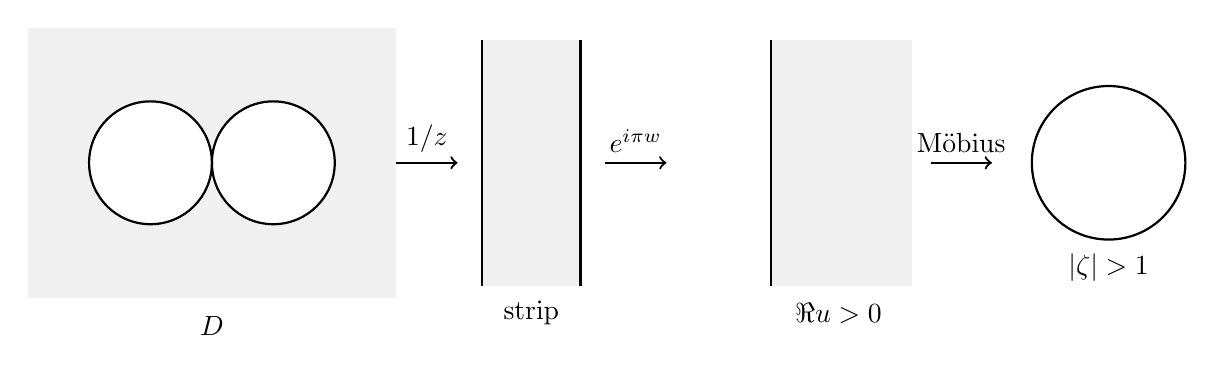
\begin{tikzpicture}[scale=0.78]
  \begin{scope}[xshift=-6cm]
    \fill[gray!12] (-3,-2.2) rectangle (3,2.2);
    \fill[white] (-1,0) circle (1);
    \fill[white] (1,0) circle (1);
    \draw[thick] (-1,0) circle (1);
    \draw[thick] (1,0) circle (1);
    \node at (0,-2.65) {$D$};
  \end{scope}
  \draw[->,thick] (-3.0,0)--(-2.0,0) node[midway,above] {$1/z$};
  \begin{scope}[xshift=-0.8cm]
    \fill[gray!12] (-0.8,-2.0) rectangle (0.8,2.0);
    \draw[thick] (-0.8,-2)--(-0.8,2);
    \draw[thick] (0.8,-2)--(0.8,2);
    \node at (0,-2.45) {strip};
  \end{scope}
  \draw[->,thick] (0.4,0)--(1.4,0) node[midway,above] {$e^{i\pi w}$};
  \begin{scope}[xshift=3.1cm]
    \fill[gray!12] (0,-2) rectangle (2.3,2);
    \draw[thick] (0,-2)--(0,2);
    \node at (1.1,-2.45) {$\Re u>0$};
  \end{scope}
  \draw[->,thick] (5.7,0)--(6.7,0) node[midway,above] {Möbius};
  \begin{scope}[xshift=8.6cm]
    \draw[thick] (0,0) circle (1.25);
    \node at (0,-1.7) {$|\zeta|>1$};
  \end{scope}
\end{tikzpicture}
\caption{For part (a), inversion turns the two circles through the origin into parallel lines; rotation/scaling and the exponential produce a half-plane, and a Möbius map sends that half-plane to the exterior of the unit circle.}
\label{fig:cp-iv-0016-two-circles-mapping-pipeline}
\end{figure}


\begin{solution}
For part (a), put
\[
w=\frac1z.
\]
The circles through the origin become
\[
|z-1|=1\iff \Re w=\frac12,
\qquad
|z+1|=1\iff \Re w=-\frac12.
\]
Thus the region exterior to both circles maps to
\[
-\frac12<\Re w<\frac12.
\]
Now set
\[
s=i\pi w.
\]
Then
\[
|\Im s|<\frac{\pi}{2},
\]
so
\[
u=e^s
\]
lies in the right half-plane. The Cayley map
\[
\Phi(u)=\frac{u+1}{u-1}
\]
maps the right half-plane to the exterior of the unit disk. Hence
\[
\boxed{
\zeta(z)
=
\frac{e^{i\pi/z}+1}{e^{i\pi/z}-1}
}
\]
is a conformal map for part (a).

For part (b), the Cayley map
\[
w=\frac{1+z}{1-z}
\]
takes the unit disk to \(\Re w>0\). The principal logarithm then gives
\[
\boxed{
\zeta(z)
=
\Log\left(\frac{1+z}{1-z}\right),
}
\]
with
\[
-\frac{\pi}{2}<\Im\zeta<\frac{\pi}{2}.
\]
Also
\[
z=0\mapsto0,\qquad
z=1\mapsto+\infty,\qquad
z=-1\mapsto-\infty.
\]

For part (c), first square:
\[
t=z^2.
\]
This maps the quarter-disk conformally onto the upper half of the unit disk, with
\[
0\mapsto0,\qquad1\mapsto1,\qquad i\mapsto-1.
\]
Next,
\[
q=\frac{1+t}{1-t}
\]
maps that upper half-disk onto the first quadrant. Squaring gives the upper half-plane:
\[
s=q^2.
\]
Now
\[
t=-1\mapsto s=0,\qquad
t=0\mapsto s=1,\qquad
t=1\mapsto s=\infty.
\]
Finally use
\[
M(s)=1-\frac1s,
\]
which sends
\[
0\mapsto\infty,\qquad1\mapsto0,\qquad\infty\mapsto1.
\]
After simplification,
\[
M\!\left(\left(\frac{1+t}{1-t}\right)^2\right)
=
\frac{4t}{(1+t)^2}.
\]
Therefore the required map is
\[
\boxed{
\zeta(z)
=
\frac{4z^2}{(1+z^2)^2}.
}
\]
It satisfies
\[
\zeta(0)=0,\qquad
\zeta(1)=1,\qquad
\zeta(i)=\infty,
\]
and maps the quarter-disk bijectively onto the upper half-plane.

The simpler expression \(2z^2/(1+z^2)\) appearing in the migrated source maps the intermediate semicircle only to a proper subdomain of the upper half-plane; the composition above gives the required onto map.
\end{solution}


\begin{problem}[CP-IV-0019]
\label{prob:cp-iv-0019}
\par\noindent\textbullet\quad Inversion in a circle is \emph{anti-conformal} (it involves complex conjugation), and the composition of two inversions is conformal; in particular, any composition of an \emph{even} number of inversions is holomorphic (hence Möbius on $\widehat{\mathbb C}$).
\end{problem}

% Designed Companion Part IV figure
% Intended for \input{...} beside the matching canonical problem.
\begin{figure}[ht]
\centering
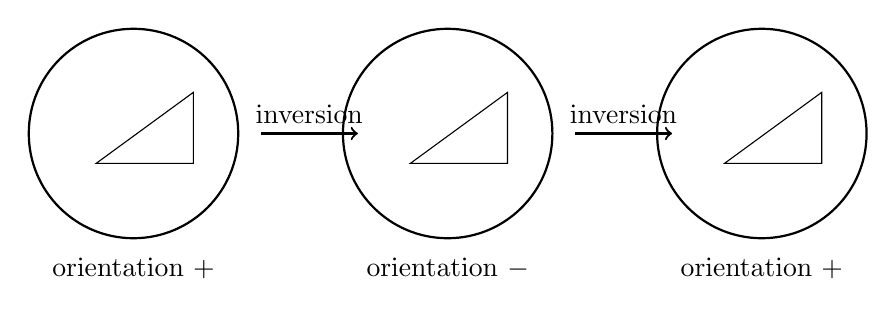
\begin{tikzpicture}[scale=0.95]
  \begin{scope}[xshift=-4.2cm]
    \draw[thick] (0,0) circle (1.4);
    \draw[->] (-0.5,-0.4)--(0.8,-0.4)--(0.8,0.55)--cycle;
    \node at (0,-1.8) {orientation $+$};
  \end{scope}
  \draw[->,thick] (-2.5,0)--(-1.2,0) node[midway,above] {inversion};
  \begin{scope}
    \draw[thick] (0,0) circle (1.4);
    \draw[->] (-0.5,-0.4)--(0.8,0.55)--(0.8,-0.4)--cycle;
    \node at (0,-1.8) {orientation $-$};
  \end{scope}
  \draw[->,thick] (1.7,0)--(3.0,0) node[midway,above] {inversion};
  \begin{scope}[xshift=4.2cm]
    \draw[thick] (0,0) circle (1.4);
    \draw[->] (-0.5,-0.4)--(0.8,-0.4)--(0.8,0.55)--cycle;
    \node at (0,-1.8) {orientation $+$};
  \end{scope}
\end{tikzpicture}
\caption{Circle inversion is anti-conformal and reverses local orientation. Composing two inversions reverses orientation twice, giving a conformal transformation; on the Riemann sphere such compositions are Möbius transformations.}
\label{fig:cp-iv-0019-two-inversions-orientation}
\end{figure}


\begin{solution}
Geometric inversion in a circle has the form
\[
I(z)
=
a+\frac{r^2}{\overline{z-a}},
\]
so it is antiholomorphic away from the center. In particular it reverses orientation.

The composition of two antiholomorphic maps is holomorphic. Thus if
\[
I_1,\ I_2
\]
are circle or line inversions, then
\[
I_2\circ I_1
\]
is conformal and orientation-preserving wherever defined. On the Riemann sphere, a bijective holomorphic conformal map is a M\"obius transformation. Therefore any composition of an even number of geometric inversions is M\"obius.

Similarly, an odd number of inversions gives an anti-M\"obius transformation. This parity distinction is exactly the orientation distinction:
\[
\text{even number of inversions}\Rightarrow\text{orientation preserved},
\]
\[
\text{odd number of inversions}\Rightarrow\text{orientation reversed}.
\]
\end{solution}


\begin{problem}[CP-IV-0023]
\label{prob:cp-iv-0023}
\par\noindent\textbullet\quad \textbf{(b)}\;
	Consider the branch defined by
	\[
	f(z) \;=\; (r_{1}r_{2})^{1/2} \, e^{\,i(\theta_{1}+\theta_{2})/2},
	\qquad -\tfrac{\pi}{2}<\theta_{1},\ \theta_{2}\le \tfrac{3\pi}{2}.
	\]
	State the values of \((\theta_{1}+\theta_{2})/2\) on either side of the imaginary axis,
	and hence compute \(f(\pm0+iy)\) in terms of \(y\) for \(y\in\mathbb{R}\).
	Deduce that the branch cut is
	\[
	S \;=\; \{\,x+iy:\ x=0,\ |y|\le 1\,\}.
	\]
	Show that \(f(z)\sim z\) as \(|z|\to\infty\)
	(i.e.\ \(f(z)/z\to 1\) as \(|z|\to\infty\)).
	Sketch the image of the cut \(z\)-plane \(\mathbb{C}\setminus S\) under the map \(\zeta=f(z)\).

	\medskip
\end{problem}

% Designed Companion Part IV figure
% Intended for \input{...} beside the matching canonical problem.
\begin{figure}[ht]
\centering
\begin{tikzpicture}[scale=1.08]
  \draw[->] (-3.0,0)--(3.0,0) node[right] {$\Re z$};
  \draw[->] (0,-2.7)--(0,2.7) node[above] {$\Im z$};
  \draw[very thick] (0,-1)--(0,1);
  \fill (0,1) circle (1.6pt) node[right] {$i$};
  \fill (0,-1) circle (1.6pt) node[right] {$-i$};
  \node[right] at (0.15,0) {$S$};
  \node at (2.05,1.25) {$f(z)\sim z$};
  \node at (0,-2.2) {$\mathbb C\setminus S$};
  \draw[dashed] (-0.55,-0.8)--(-0.55,0.8);
  \draw[dashed] (0.55,-0.8)--(0.55,0.8);
\end{tikzpicture}
\caption{The selected branch has the finite slit $S=\{iy:|y|\le1\}$ joining the branch points $\pm i$. Boundary values are taken on the two sides of the slit, while the branch behaves as $f(z)\sim z$ at infinity.}
\label{fig:cp-iv-0023-finite-imaginary-branch-cut}
\end{figure}


\begin{solution}
Again write
\[
z-i=r_1e^{i\theta_1},
\qquad
z+i=r_2e^{i\theta_2},
\]
but now take
\[
-\frac{\pi}{2}<\theta_1,\theta_2\le\frac{3\pi}{2}.
\]
For \(-1<y<1\), approach \(z=iy\) from the right. Then
\[
\theta_1\to-\frac{\pi}{2},
\qquad
\theta_2\to\frac{\pi}{2},
\]
so
\[
\frac{\theta_1+\theta_2}{2}\to0
\]
and
\[
f(+0+iy)=\sqrt{1-y^2}.
\]
Approaching from the left forces \(\theta_1\) to wrap to \(3\pi/2\), while \(\theta_2\to\pi/2\). Hence
\[
\frac{\theta_1+\theta_2}{2}\to\pi,
\]
and
\[
f(-0+iy)=-\sqrt{1-y^2}.
\]
Thus the jump occurs precisely on
\[
S=\{iy:|y|\le1\}.
\]
Outside that segment the boundary values agree, so the branch cut is exactly \(S\).

Since
\[
f(z)^2=z^2+1,
\]
we have
\[
f(z)
=
z\sqrt{1+\frac1{z^2}},
\]
and the selected branch satisfies
\[
f(z)\sim z
\qquad(|z|\to\infty).
\]

The two sides of the slit are mapped to the two sides of the real segment \([-1,1]\):
\[
f(+0+iy)=+\sqrt{1-y^2},
\qquad
f(-0+iy)=-\sqrt{1-y^2}.
\]
Consequently the branch gives a conformal map
\[
\boxed{
\mathbb C\setminus[-i,i]
\longrightarrow
\mathbb C\setminus[-1,1].
}
\]
The real axis maps to
\[
(-\infty,-1]\cup[1,\infty),
\]
and the outer imaginary rays map to the imaginary axis.
\end{solution}


\begin{problem}[CP-IV-0027]
\label{prob:cp-iv-0027}
(i) Let $\Log$ denote the principal branch of $\log$ on $\mathbb C\setminus(-\infty,0]$.
For $z\in\mathbb C$, show that $n\Log(1+z/n)$ is defined for $n$ sufficiently large and that
$n\Log(1+z/n)\to z$. Deduce $\displaystyle\lim_{n\to\infty}\bigl(1+\frac{z}{n}\bigr)^n=e^{z}$.
\smallskip

(ii) Defining $z^\alpha:=\exp(\alpha\Log z)$ for $\alpha\in\mathbb C$ and $z\notin\mathbb R_{\le 0}$,
show $\dfrac{d}{dz}z^\alpha=\alpha z^{\alpha-1}$. Does $(zw)^\alpha=z^\alpha w^\alpha$ always hold?
\end{problem}

\begin{solution}
\emph{(i) Limit of $n\Log(1+z/n)$.}
For fixed $z$, choose $n$ large so that $1+\frac{z}{n}$ lies in a small disc around $1$
disjoint from $(-\infty,0]$, hence $\Log$ is holomorphic there. Since
\[
\lim_{u\to 0}\frac{\Log(1+u)}{u}=1,
\]
we get, with $u=z/n$,
\[
n\Log\Bigl(1+\frac{z}{n}\Bigr)
= z\,\frac{\Log(1+z/n)}{z/n}\ \longrightarrow\ z.
\]
Therefore
\[
\lim_{n\to\infty}\Bigl(1+\frac{z}{n}\Bigr)^n
=\lim_{n\to\infty}\exp\!\Bigl(n\Log\bigl(1+\tfrac{z}{n}\bigr)\Bigr)
=\exp(z)=e^z.
\]

\emph{(ii) Derivative and multiplicative law.}
On $\mathbb C\setminus(-\infty,0]$, $\Log$ is holomorphic with $(\Log z)'=1/z$, hence
\[
\frac{d}{dz}z^\alpha
=\frac{d}{dz}\exp(\alpha\Log z)
=\exp(\alpha\Log z)\,\alpha\,\frac1z
=\alpha z^{\alpha-1}.
\]

For $z,w$ in the domain of $\Log$, in general
\[
\Log(zw)=\Log z+\Log w-2\pi i\,k,\qquad k\in\mathbb Z,
\]
so
\[
(zw)^\alpha
=\exp\!\bigl(\alpha\Log(zw)\bigr)
=z^\alpha w^\alpha\,e^{-2\pi i\alpha k}.
\]
Thus $(zw)^\alpha=z^\alpha w^\alpha$ holds when no branch jump occurs
(\,$-\pi<\Arg z+\Arg w<\pi$\,), or when $\alpha\in\mathbb Z$; otherwise it can fail.

\emph{Counterexample.} With $\alpha=\tfrac12$ and $z=w=e^{3\pi i/4}$,
$\Log z=\Log w=i\,3\pi/4$ but $\Log(zw)=-i\pi/2$, hence
$z^\alpha w^\alpha=e^{i\,3\pi/4}\neq e^{-i\pi/4}=(zw)^\alpha$.
\end{solution}

\begin{problem}[CP-IV-0036]
\label{prob:cp-iv-0036}
Show that the following functions do not have antiderivatives on the indicated domains:
\[
\text{(a)}\; f(z)=\frac{1}{z}-\frac{1}{z-1}\quad\text{on } \{\,0<|z|<1\,\},\qquad
\text{(b)}\; g(z)=\frac{z}{1+z^{2}}\quad\text{on } \{\,1<|z|<\infty\,\}.
\]

We collect the standard criteria we will use.

	\par\noindent\textbullet\quad \textbf{Path-independence / primitives.} If $h$ is holomorphic on a domain $U$ and has a primitive $H$ on $U$ (i.e.\ $H'=h$), then
	\[
	\int_\gamma h(z)\,dz=0 \quad \text{for every closed curve }\gamma\subset U,
	\]
	and conversely, if every closed integral vanishes on $U$, then $h$ has a primitive on $U$.

	\par\noindent\textbullet\quad \textbf{Residue theorem (basic form).} Let $h$ be meromorphic on an open set containing a positively oriented simple closed curve $\gamma$ and its interior, with no poles on $\gamma$. Then
	\[
	\int_\gamma h(z)\,dz = 2\pi i \sum_{a\in \mathrm{Int}(\gamma)} \operatorname{Res}(h;a).
	\]
	For a \emph{simple pole} at $a$, $\displaystyle \operatorname{Res}(h;a)=\lim_{z\to a}(z-a)h(z)$.
	(Equivalently, if $h=p/q$ with $p,q$ holomorphic and $q'(a)\neq 0$, then
	$\displaystyle \operatorname{Res}(h;a)=\frac{p(a)}{q'(a)}$.)

	\par\noindent\textbullet\quad \textbf{No global log $\Rightarrow$ no primitive.} A holomorphic $h$ on $U$ has a holomorphic logarithm $\log h$ on $U$ iff $\int_\gamma h'(z)/h(z)\,dz=0$ for every closed $\gamma\subset U$ (equivalently, $h$ has no zeros with nonzero winding number around loops in $U$). In particular, if a holomorphic expression forces a nontrivial jump of argument around a hole, then a single-valued primitive involving $\log$ cannot exist on $U$.

	\par\noindent\textbullet\quad \textbf{Winding number version.} If $\gamma$ is a positively oriented circle $|z-z_0|=r$, then
	\[
	\frac{1}{2\pi i}\int_\gamma \frac{dz}{z-z_0}=1.
	\]
	More generally, for any closed $\gamma$ and $a\notin \gamma$, $\displaystyle \frac{1}{2\pi i}\int_\gamma \frac{dz}{z-a}$
	equals the winding number of $\gamma$ around $a$.
\end{problem}

% Designed Companion Part IV figure
% Intended for \input{...} beside the matching canonical problem.
\begin{figure}[ht]
\centering
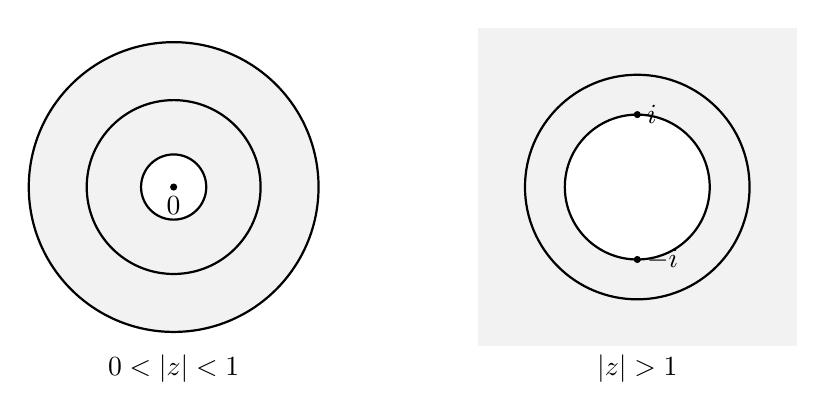
\begin{tikzpicture}[scale=0.92]
  \begin{scope}[xshift=-3.2cm]
    \fill[gray!10] (0,0) circle (2.0);
    \fill[white] (0,0) circle (0.45);
    \draw[thick] (0,0) circle (2.0);
    \draw[thick] (0,0) circle (0.45);
    \draw[->,thick] (0,0) circle (1.2);
    \fill (0,0) circle (1.4pt) node[below] {$0$};
    \node at (0,-2.5) {$0<|z|<1$};
  \end{scope}
  \begin{scope}[xshift=3.2cm]
    \fill[gray!10] (-2.2,-2.2) rectangle (2.2,2.2);
    \fill[white] (0,0) circle (1.0);
    \draw[thick] (0,0) circle (1.0);
    \draw[->,thick] (0,0) circle (1.55);
    \fill (0,1) circle (1.4pt) node[right] {$i$};
    \fill (0,-1) circle (1.4pt) node[right] {$-i$};
    \node at (0,-2.5) {$|z|>1$};
  \end{scope}
\end{tikzpicture}
\caption{Each domain has a noncontractible loop. Integrating around such a loop detects the logarithmic/winding obstruction and proves that the indicated holomorphic function cannot possess a global primitive.}
\label{fig:cp-iv-0036-primitive-obstruction-loops}
\end{figure}


\begin{solution}
\emph{(a) $f(z)=\dfrac{1}{z}-\dfrac{1}{z-1}$ on $0<|z|<1$.}
Let $\gamma_r$ be the positively oriented circle $|z|=r$ with $0<r<1$. Then $\gamma_r\subset\{0<|z|<1\}$,
and the only singularity of $f$ in the interior is $z=0$ (simple pole with residue $1$). Thus, by the residue theorem,
\[
\int_{\gamma_r} f(z)\,dz
= 2\pi i\,\operatorname{Res}(f;0)
= 2\pi i \neq 0.
\]
If $f$ had a primitive on the annulus $0<|z|<1$, every closed integral would vanish—a contradiction. Hence no primitive exists there.

\medskip
\emph{(b) $g(z)=\dfrac{z}{1+z^{2}}$ on $1<|z|<\infty$.}
Let $\Gamma_R$ be the circle $|z|=R>1$. Then $\Gamma_R\subset\{1<|z|<\infty\}$.
The function $g$ has simple poles at $\pm i$ (both lie inside $\Gamma_R$ and off the curve).
Using the simple-pole formula with $p(z)=z$, $q(z)=1+z^2$,
\[
\operatorname{Res}(g;i)=\frac{p(i)}{q'(i)}=\frac{i}{2i}=\frac{1}{2},\qquad
\operatorname{Res}(g;-i)=\frac{p(-i)}{q'(-i)}=\frac{-i}{-2i}=\frac{1}{2}.
\]
Hence
\[
\int_{\Gamma_R} g(z)\,dz = 2\pi i\Big(\tfrac12+\tfrac12\Big)=2\pi i\neq 0,
\]
so $g$ cannot have a primitive on the exterior domain $\{1<|z|<\infty\}$.
\end{solution}

\begin{problem}[CP-IV-0043]
\label{prob:cp-iv-0043}
\par\noindent\textbullet\quad \textbf{(a)}\;
	Show that, if \(\zeta^{2}=z^{2}+1\) and
	\[
	z = i + r_{1}e^{i\theta_{1}} = -\,i + r_{2}e^{i\theta_{2}},
	\qquad r_{1},r_{2}>0,\ \theta_{1},\theta_{2}\in\mathbb{R},
	\]
	then
	\[
	\zeta \;=\; \pm\,(r_{1}r_{2})^{1/2}\,e^{\,i(\theta_{1}+\theta_{2})/2}.
	\]
	Explain briefly why \(z=\pm i\) are the branch points of the multifunction \((z^{2}+1)^{1/2}\).

	\medskip
\end{problem}

\begin{solution}
Since
\[
z^2+1=(z-i)(z+i),
\]
and
\[
z-i=r_1e^{i\theta_1},
\qquad
z+i=r_2e^{i\theta_2},
\]
we obtain
\[
\zeta^2
=
r_1r_2e^{i(\theta_1+\theta_2)}.
\]
Taking square roots gives the two values
\[
\boxed{
\zeta
=
\pm (r_1r_2)^{1/2}
e^{\,i(\theta_1+\theta_2)/2}.
}
\]

The points \(z=\pm i\) are precisely the zeros of \(z^2+1\), and both zeros are simple. If one analytically continues a local square root once around either simple zero, the argument of \(z^2+1\) increases by \(2\pi\), so the square root acquires the factor
\[
e^{i\pi}=-1.
\]
Thus the two values are interchanged after one circuit. Hence no single-valued holomorphic square root can be defined on a punctured neighborhood of either point, and \(z=\pm i\) are the branch points of \((z^2+1)^{1/2}\).
\end{solution}


\begin{problem}[CP-IV-0052]
\label{prob:cp-iv-0052}
(restated).

Let $p(z)=z^{5}+z$.

	\par\noindent\textbullet\quad Find all $z$ with $|z|=1$ such that $\Im p(z)=0$.
	\par\noindent\textbullet\quad Compute $\Re p(z)$ at the points from (a).
	\par\noindent\textbullet\quad Sketch the curve $p\circ\gamma$ where $\gamma(t)=e^{2\pi i t}$.
	\par\noindent\textbullet\quad Using your sketch, determine for each real $x$ the number of solutions $z$ (counted with multiplicity) to $p(z)=x$ with $|z|<1$.

\paragraph{6. The map $p(z)=z^{5}+z$ on the unit circle.}
Let $z=e^{i\theta}$.
\[
p(e^{i\theta})=e^{5i\theta}+e^{i\theta}
=2\cos(2\theta)\,e^{i3\theta}.
\]

\emph{(a) Real axis crossings.} $\Im p=0 \iff \sin(5\theta)+\sin\theta=2\sin(3\theta)\cos(2\theta)=0$,
so $\theta=\frac{m\pi}{3}$ ($m=0,\dots,5$) or $\theta=\frac{\pi}{4}+\frac{k\pi}{2}$ ($k=0,1,2,3$).

\emph{(b) Real parts at these points.} $\Re p=\cos(5\theta)+\cos\theta=2\cos(3\theta)\cos(2\theta)$.
For $\cos(2\theta)=0$, $\Re p=0$; for $\theta=\frac{m\pi}{3}$ the values are $2,1,-1,-2,-1,1$.

\emph{(c) Sketch.} The curve $p(\gamma)$ ($\gamma(t)=e^{2\pi it}$) is a three-petal curve of maximal radius $2$, meeting the real axis at $-2,-1,0,1,2$.

\emph{(d) Number of solutions to $z^{5}+z=x$ with $|z|<1$, $x\in\mathbb R$.}
By the argument principle, the number equals the winding number of $p(\gamma)$ about $x$. From the sketch,
\[
N(x)=
\begin{cases}
	0, & |x|>2,\\[2pt]
	1, & 1<|x|<2,\\[2pt]
	2, & 0<|x|<1,\\[2pt]
	1, & x=0\ \text{(one interior root; the other four sit on/near the boundary)}.
\end{cases}
\]


\emph{Mellin/keyhole integrals.}
For $0<\Re\mu<2$ and $0<\phi<\pi$,
\[
\int_{0}^{\infty}\frac{x^{\mu-1}}{x^{2}+2x\cos\phi+1}\,dx
=\frac{\pi\,\sin(\mu\phi)}{\sin(\pi\mu)\,\sin\phi}.
\]
Derivation uses a keyhole contour with the branch of $\Log$ on $\mathbb C\setminus(-\infty,0]$.

\smallskip
\emph{Definitions.}
Mellin transform: $\mathcal M[f](s)=\int_{0}^{\infty}x^{s-1}f(x)\,dx$.
Keyhole contour: a contour encircling the positive real axis to capture the $2\pi i$ jump of the logarithm.

\medskip
\emph{Cauchy’s root bound (polynomials).}
For $p(z)=z^{n}+a_{n-1}z^{n-1}+\cdots+a_0$, every root satisfies
\[
|z|<1+\max_{0\le k\le n-1}|a_k|=:A+1.
\]
Idea: on $|z|=R>A$, $|z|^{n}>\sum_{k\le n-1}|a_k||z|^{k}$, hence $|p(z)|>0$.

\smallskip
\emph{Rouché’s theorem (context).}
If $f,g$ are holomorphic and $|f|>|g|$ on a simple closed curve, then $f$ and $f+g$ have the same number of zeros inside.

\medskip
\emph{Argument principle.}
If $f$ is meromorphic with no zeros/poles on a positively oriented simple closed curve $\gamma$,
\[
N-P=\frac{1}{2\pi i}\int_{\gamma}\frac{f'(z)}{f(z)}\,dz=\frac{1}{2\pi}\Delta_{\gamma}\arg f.
\]
For $f(z)=p(z)-x$ (polynomial minus real parameter), $P=0$, and the integral counts the zeros of $p(z)=x$ inside.

\smallskip
\emph{Unit circle parametrization for $p(z)=z^5+z$.}
For $z=e^{i\theta}$,
\[
p(e^{i\theta})=e^{i5\theta}+e^{i\theta}
=2\cos(2\theta)\,e^{i3\theta}.
\]
Thus $p(\partial\mathbb D)$ is a three-petal curve (max radius $2$) with real-axis crossings at $-2,-1,0,1,2$.

\medskip

\emph{(4) Mellin use.}
With $x^{2}+x+1=x^{2}+2x\cos(\pi/3)+1$, set $\mu=\alpha+1$, $\phi=\pi/3$:
\[
\int_{0}^{\infty}\frac{x^{\alpha}}{x^{2}+x+1}\,dx
=\frac{2\pi}{\sqrt3}\,\frac{\sin\!\big((\alpha+1)\pi/3\big)}{\sin(\pi\alpha)}
\quad(-1<\alpha<1,\ \alpha\neq 0).
\]

\smallskip
\emph{(5) Root bound.}
If $p(z)=z^{4}-7z^{2}+10$, then $A=\max\{7,10\}=10$, so every root has $|z|<11$.

\smallskip
\emph{(6) Winding numbers for $z^5+z=x$.}
From $p(e^{i\theta})=2\cos(2\theta)e^{i3\theta}$, the number of zeros of $z^5+z=x$ in $|z|<1$ (counting multiplicity) is
\[
N(x)=
\begin{cases}
	0, & |x|>2,\\
	1, & 1<|x|<2,\\
	2, & 0<|x|<1,\\
	1, & x=0.
\end{cases}
\]


\emph{Setup.}
For integrals of the form
\[
\int_{0}^{\infty} x^{\mu-1} F(x)\,dx,
\]
choose the branch $z^{\mu-1}=e^{(\mu-1)\Log z}$ with $\Log z=\log|z|+i\Arg z$ and a branch cut along a ray (typically the positive or negative real axis). The \emph{keyhole contour} $\Gamma_{R,\varepsilon}$ wraps once around this cut:

	\par\noindent\textbullet\quad upper bank: $x\in[\varepsilon,R]$ along the ray, angle $0$,
	\par\noindent\textbullet\quad large circle $C_R$: $|z|=R$, counterclockwise,
	\par\noindent\textbullet\quad lower bank: $x\in[R,\varepsilon]$ just below the ray, angle $2\pi$,
	\par\noindent\textbullet\quad small circle $c_\varepsilon$: $|z|=\varepsilon$, counterclockwise.

Along the lower bank, $z^{\mu-1}$ picks up the factor $e^{2\pi i(\mu-1)}$.

\medskip
\emph{Vanishing of circular arcs.}
If $f(z)=z^{\mu-1}/Q(z)$ and $Q$ is a polynomial, then
\[
\int_{C_R} f(z)\,dz \to 0 \quad (R\to\infty) \ \text{if}\ \Re\mu<\deg Q,
\qquad
\int_{c_\varepsilon} f(z)\,dz \to 0 \quad (\varepsilon\to0) \ \text{if}\ \Re\mu>0.
\]
Hence one typically assumes $0<\Re\mu<\deg Q$.

\medskip
\emph{Bank contributions and jump factor.}
Let $I=\displaystyle\int_{0}^{\infty}\frac{x^{\mu-1}}{Q(x)}\,dx$.
Upper bank contributes $I$. Lower bank contributes $-e^{2\pi i(\mu-1)} I$ (reversed orientation).
Thus
\[
\int_{\Gamma_{R,\varepsilon}} \frac{z^{\mu-1}}{Q(z)}\,dz
\;\xrightarrow[R\to\infty]{\varepsilon\to0}\;
\bigl(1-e^{2\pi i(\mu-1)}\bigr)\,I
=2i\,e^{i\pi(\mu-1)}\sin(\pi\mu)\,I.
\]

\medskip
\emph{Residue theorem.}
If $Q$ has zeros $a_k$ not on the cut, then
\[
\int_{\Gamma_{R,\varepsilon}} \frac{z^{\mu-1}}{Q(z)}\,dz
\to 2\pi i \sum_k \operatorname{Res}\!\left(\frac{z^{\mu-1}}{Q(z)}; a_k\right).
\]
Equate with the bank expression to solve for $I$.

\medskip
\emph{Example 1 (Euler’s Beta integral).}
For $Q(z)=1+z$ and $0<\Re\mu<1$,
\[
\int_{0}^{\infty}\frac{x^{\mu-1}}{1+x}\,dx
=\frac{\pi}{\sin(\pi\mu)}.
\]

\medskip
\emph{Example 2 (quadratic denominator).}
For $Q(z)=z^{2}+2z\cos\phi+1=(z-e^{i\phi})(z-e^{-i\phi})$ with $0<\phi<\pi$ and $0<\Re\mu<2$,
\[
\int_{0}^{\infty}\frac{x^{\mu-1}}{x^{2}+2x\cos\phi+1}\,dx
=\frac{\pi\,\sin(\mu\phi)}{\sin(\pi\mu)\,\sin\phi}.
\]
\emph{Sketch.} The poles are at $e^{\pm i\phi}$; compute
\[
\operatorname{Res}\left(\frac{z^{\mu-1}}{(z-e^{i\phi})(z-e^{-i\phi})};e^{i\phi}\right)
=\frac{e^{i\phi(\mu-1)}}{2i\sin\phi},\quad
\operatorname{Res}(\cdots;e^{-i\phi})=\frac{e^{-i\phi(\mu-1)}}{-2i\sin\phi}.
\]
Sum and equate with the bank expression.

\medskip
\emph{Pitfalls.}
(1) Be consistent with the branch cut; (2) ensure the circular arcs vanish (conditions on $\Re\mu$);
(3) avoid poles on the cut (move the cut, or indent and take principal values if needed).
\end{problem}

% Designed Companion Part IV figure
% Intended for \input{...} beside the matching canonical problem.
\begin{figure}[ht]
\centering
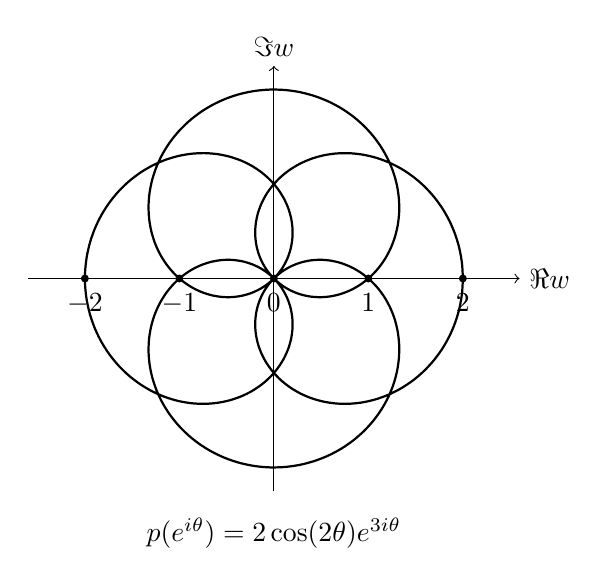
\begin{tikzpicture}[scale=1.2]
  \draw[->] (-2.6,0)--(2.6,0) node[right] {$\Re w$};
  \draw[->] (0,-2.25)--(0,2.25) node[above] {$\Im w$};
  \draw[thick,domain=0:360,samples=240,smooth,variable=\t]
    plot ({2*cos(2*\t)*cos(3*\t)},{2*cos(2*\t)*sin(3*\t)});
  \foreach \x/\lab in {-2/-2,-1/-1,0/0,1/1,2/2} {
    \fill (\x,0) circle (1.2pt);
    \node[below] at (\x,-0.06) {$\lab$};
  }
  \node at (0,-2.7) {$p(e^{i\theta})=2\cos(2\theta)e^{3i\theta}$};
\end{tikzpicture}
\caption{The image $p(\partial\mathbb D)$ is a three-petal curve with real-axis crossings at $-2,-1,0,1,2$. Winding numbers of this curve about a real point $x$ count the roots of $p(z)=x$ inside the unit disk.}
\label{fig:cp-iv-0052-three-petal-image-curve}
\end{figure}


\begin{solution}
Put \(z=e^{i\theta}\). Then
\[
p(e^{i\theta})
=
e^{5i\theta}+e^{i\theta}
=
2\cos(2\theta)e^{i3\theta}.
\]
Therefore
\[
\Im p(e^{i\theta})
=
2\cos(2\theta)\sin(3\theta).
\]
Hence the image lies on the real axis exactly when
\[
\sin(3\theta)=0
\quad\text{or}\quad
\cos(2\theta)=0.
\]
Thus
\[
\theta=\frac{m\pi}{3}\quad(m=0,\ldots,5),
\]
or
\[
\theta=\frac{\pi}{4}+\frac{k\pi}{2}\quad(k=0,\ldots,3).
\]

Also
\[
\Re p(e^{i\theta})
=
2\cos(2\theta)\cos(3\theta).
\]
For \(\cos(2\theta)=0\), this is \(0\). For
\(\theta=m\pi/3\), the values are
\[
2,\ 1,\ -1,\ -2,\ -1,\ 1.
\]
Thus the real-axis crossings are
\[
-2,\,-1,\,0,\,1,\,2.
\]

The polar equation
\[
p(e^{i\theta})=2\cos(2\theta)e^{i3\theta}
\]
shows that \(p(\partial\mathbb D)\) is a three-petal curve. The number of roots of
\[
z^5+z=x
\]
in \(|z|<1\) is the winding number of this curve about the real point \(x\), provided \(x\) is not itself on the curve. Reading the winding number of the three petals gives
\[
\boxed{
N(x)=
\begin{cases}
0,& |x|>2,\\[2mm]
1,& 1<|x|<2,\\[2mm]
3,& 0<|x|<1.
\end{cases}}
\]

At the crossing values, roots lie on \(|z|=1\), so they must be treated separately:
\[
N(\pm2)=0,\qquad
N(\pm1)=1,\qquad
N(0)=1.
\]
Indeed, when \(x=0\),
\[
z^5+z=z(z^4+1),
\]
so \(z=0\) is the unique root strictly inside the unit disk and the four roots of \(z^4=-1\) lie on the unit circle.

Thus the value \(2\) sometimes quoted for \(0<|x|<1\) is not the interior root count; the correct winding number there is \(3\).
\end{solution}


\begin{problem}[CP-IV-0086]
\label{prob:cp-iv-0086}
\par\noindent\textbullet\quad \textbf{Essential:} neither removable nor pole. The Laurent expansion at $a$ then has infinitely many negative powers.

\medskip
\emph{Casorati--Weierstrass \& Picard (context for Problem 9).}
If $a$ is an essential singularity of $f$, then the image of any punctured neighborhood of $a$ is dense in $\mathbb C$
(Casorati--Weierstrass). A stronger statement (Great Picard) says that near an essential singularity $f$ attains every complex value, with at most one exception, infinitely often.

\medskip
\emph{Identity theorem \& isolated zeros.}
If $f,g$ are holomorphic on a domain $U$ and $f=g$ on a set with a limit point in $U$, then $f\equiv g$ on $U$.
Consequently, a nonzero holomorphic function on $U$ has zeros that do not accumulate in $U$.

\medskip
\emph{Path independence and primitives (for Problem 10).}
If $\omega(z)\,dz$ is holomorphic on a simply connected domain $D$, then
\[
F(z):=\int_{z_0}^{z}\omega(\zeta)\,d\zeta
\]
is well defined (independent of path), holomorphic on $D$, and satisfies $F'=\omega$.
In particular, if $0\notin D$, the $1$-form $d\zeta/\zeta$ has the primitive
$F(z)=\int_{z_0}^z \frac{d\zeta}{\zeta}$ on $D$, so $e^{F}$ gives a single-valued branch of the logarithm.

\smallskip
\emph{Winding number criterion for a logarithm.}
A holomorphic, nowhere–vanishing function $g$ on a domain $D$ admits a holomorphic branch of $\Log g$ on $D$
iff $\displaystyle \int_{\gamma} \frac{g'}{g}\,dz=0$ for every closed curve $\gamma\subset D$;
equivalently, $g(\gamma)$ has winding number $0$ about $0$ for all such $\gamma$.
When $D$ is simply connected and $g$ never vanishes, a branch of $\Log g$ always exists.

\medskip
\emph{Power series, radius of convergence, and natural boundaries (for Problem 11).}
A power series $\sum_{n\ge0} a_n z^n$ has a radius of convergence $R\in[0,\infty]$ determined by the Cauchy--Hadamard formula.
It defines an analytic function on $|z|<R$ and cannot be analytically continued across points where the function has a singularity.
A Jordan curve $\Gamma$ is a \emph{natural boundary} for $f$ if no analytic continuation of $f$ exists across \emph{any} point of $\Gamma$.

\smallskip
\emph{Hadamard gap theorem (lacunary series).}
If $f(z)=\sum_{k\ge1} a_k z^{n_k}$ with strictly increasing exponents $(n_k)$ satisfying
$\displaystyle \liminf_{k\to\infty} \frac{n_{k+1}}{n_k}>1$ (``Hadamard gaps''),
then the circle of convergence $|z|=R$ is a \emph{natural boundary} for $f$ (unless $f$ is a polynomial).
In particular, for $n_k=2^k$ (ratio $=2$) the unit circle is a natural boundary when $R=1$.

\medskip
\emph{Dense boundary singularities via functional identities (alternate route for Problem 11).}
If a function $f$ on $|z|<1$ satisfies identities of the form
\[
(1-z^{N})\,f(z)=P_N(z)\qquad (N\in\mathbb N),
\]
with $P_N$ polynomial and $N\to\infty$, then every $N$-th root of unity
is a singularity (unless canceled), and the union of these roots for $N\to\infty$ is dense on $|z|=1$.
Hence $|z|=1$ is a natural boundary (no analytic continuation across any boundary point).
\end{problem}

% Designed Companion Part IV figure
% Intended for \input{...} beside the matching canonical problem.
\begin{figure}[ht]
\centering
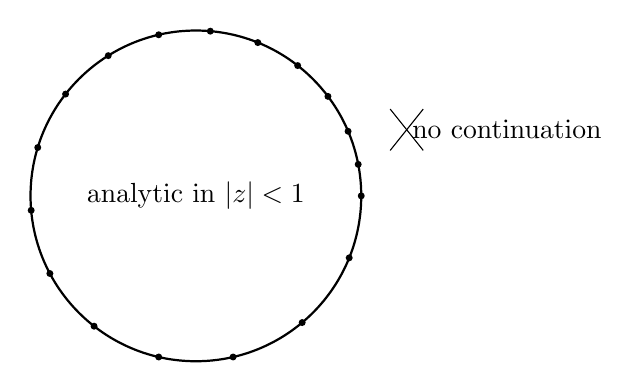
\begin{tikzpicture}[scale=1.05]
  \draw[thick] (0,0) circle (2);
  \foreach \a in {0,11,23,37,52,68,85,103,122,142,163,185,208,232,257,283,310,338} {
    \fill ({2*cos(\a)},{2*sin(\a)}) circle (1.2pt);
  }
  \node at (0,0) {analytic in $|z|<1$};
  \node[right] at (2.5,0.8) {no continuation};
  \draw (2.35,0.55)--(2.75,1.05);
  \draw (2.75,0.55)--(2.35,1.05);
\end{tikzpicture}
\caption{For a lacunary series such as one with exponents $2^k$, the unit circle is a natural boundary. Singular behavior is dense on $|z|=1$, so analytic continuation is blocked across every boundary point.}
\label{fig:cp-iv-0086-natural-boundary-unit-circle}
\end{figure}


\begin{solution}
An isolated singularity \(a\) is essential exactly when its Laurent series
\[
f(z)=\sum_{n=-\infty}^{\infty}c_n(z-a)^n
\]
contains infinitely many nonzero negative-power terms. If there are none, the singularity is removable; if only finitely many occur, it is a pole. Hence the three cases are mutually exclusive and exhaustive.

For a nowhere-vanishing holomorphic function \(g\) on a domain \(D\), a holomorphic logarithm \(L\) with
\[
e^L=g
\]
exists exactly when the holomorphic \(1\)-form
\[
\frac{g'}{g}\,dz
\]
has zero period around every closed curve:
\[
\oint_\gamma \frac{g'}{g}\,dz=0.
\]
Indeed, if \(L\) exists then \(L'=g'/g\), so all periods vanish. Conversely, if the periods vanish, then
\[
L(z)=\int_{z_0}^z\frac{g'(\zeta)}{g(\zeta)}\,d\zeta
\]
is path independent; after adding a constant one obtains \(e^L=g\). In particular, every nowhere-zero holomorphic function on a simply connected domain admits a holomorphic logarithm.

For essential singularities, Casorati--Weierstrass says that the image of every punctured neighborhood is dense in \(\mathbb C\), while Great Picard strengthens this to attainment of every complex value, with at most one exception, infinitely often.

Finally, for a lacunary power series
\[
f(z)=\sum_{k\ge1}a_kz^{n_k}
\]
with
\[
\liminf_{k\to\infty}\frac{n_{k+1}}{n_k}>1,
\]
Hadamard's gap theorem makes the circle of convergence a natural boundary (unless the series terminates). In particular, exponents \(n_k=2^k\) have ratio \(2\), so when the radius of convergence is \(1\), the unit circle is a natural boundary.
\end{solution}


\begin{problem}[CP-IV-0107]
\label{prob:cp-iv-0107}
(Conformal equivalences and a harmonic function).

Find conformal equivalences between the following pairs of domains:

	\par\noindent\textbullet\quad The sector
	\[
	S_1=\{\,z\in\mathbb{C} : -\tfrac{\pi}{4}<\Arg z<\tfrac{\pi}{4}\,\}
	\]
	and the open unit disc
	\[
	\mathbb{D}=D(0,1)=\{\,w\in\mathbb{C}:|w|<1\,\}.
	\]

	\par\noindent\textbullet\quad The lens
	\[
	L=\{\,z\in\mathbb{C} : |z-1|<\sqrt{2}\ \text{and}\ |z+1|<\sqrt{2}\,\}
	\]
	and $\mathbb{D}$.

	\par\noindent\textbullet\quad The strip
	\[
	S=\{\,z\in\mathbb{C} : 0<\Im z<1\,\}
	\]
	and the quadrant
	\[
	Q=\{\,w\in\mathbb{C} : \Re w>0,\ \Im w>0\,\}.
	\]

\noindent
By considering a suitable bounded solution of Laplace's equation $u_{xx}+u_{yy}=0$ on $S$,
find a non-constant harmonic function on $Q$ which is constant on its boundary axes.
\end{problem}

\begin{solution}
For the sector
\[
S_1=\left\{z:-\frac{\pi}{4}<\operatorname{Arg}z<\frac{\pi}{4}\right\},
\]
the squaring map sends \(S_1\) biholomorphically onto the right half-plane:
\[
z\longmapsto z^2,
\qquad
-\frac{\pi}{2}<\operatorname{Arg}(z^2)<\frac{\pi}{2}.
\]
The Cayley map
\[
\xi\longmapsto\frac{\xi-1}{\xi+1}
\]
takes the right half-plane onto \(\mathbb D\). Hence
\[
\boxed{
F_1(z)=\frac{z^2-1}{z^2+1}
}
\]
is a conformal equivalence \(S_1\to\mathbb D\).

For the lens
\[
L=\{|z-1|<\sqrt2,\ |z+1|<\sqrt2\},
\]
the two boundary circles meet at \(z=\pm i\) at right angles. Put
\[
u(z)=-\,\frac{z-i}{z+i}.
\]
The two boundary circles become the two rays
\[
\operatorname{Arg}u=\pm\frac{\pi}{4},
\]
and the lens, which contains \(z=0\), becomes the sector
\[
|\operatorname{Arg}u|<\frac{\pi}{4}.
\]
Therefore \(u^2\) maps \(L\) onto the right half-plane, and
\[
\boxed{
F_2(z)
=
\frac{u(z)^2-1}{u(z)^2+1},
\qquad
u(z)=-\frac{z-i}{z+i},
}
\]
maps \(L\) biholomorphically onto \(\mathbb D\).

For the strip
\[
S=\{0<\Im z<1\},
\]
the map
\[
\boxed{
F_3(z)=e^{\pi z/2}
}
\]
has argument
\[
0<\operatorname{Arg}F_3(z)<\frac{\pi}{2},
\]
while its modulus ranges through all positive values. Hence \(F_3\) maps \(S\) biholomorphically onto the quadrant
\[
Q=\{\Re w>0,\ \Im w>0\}.
\]

Now
\[
v(z)=\Im z
\]
is a bounded nonconstant harmonic function on \(S\), with boundary values \(0\) and \(1\) on the two horizontal boundary lines. Since
\[
F_3^{-1}(w)=\frac{2}{\pi}\Log w
\]
on \(Q\), its pullback is
\[
\boxed{
V(w)=\frac{2}{\pi}\operatorname{Arg}w.
}
\]
This is harmonic on \(Q\), equals \(0\) on the positive real axis, and equals \(1\) on the positive imaginary axis.
\end{solution}


\begin{problem}[CP-IV-0112]
\label{prob:cp-iv-0112}
(restated).

Consider the lacunary series
\[
f(z)=\sum_{n=1}^{\infty} z^{2^{n}} .
\]
Show that it defines an analytic function on $D(0,1)$ but admits no analytic continuation across any point of $|z|=1$.

\medskip
\end{problem}

\begin{solution}
\par\medskip\noindent\textbf{Solution to Problem 11.}\quad 
The series converges absolutely and uniformly on compact subsets of $D(0,1)$, so $f$ is analytic there.
Moreover, for $m\ge 1$,
\[
(1-z^{2^{m}})f(z)=\sum_{j=1}^{m-1} z^{2^{j}},
\]
so each $2^{m}$-th root of unity is a singularity of $f$ (unless trivially canceled).
As the union $\bigcup_{m\ge 1}\{\zeta:\zeta^{2^{m}}=1\}$ is dense on $|z|=1$, $|z|=1$ is a \emph{natural boundary}:
no analytic continuation is possible across any boundary point.
\end{solution}

\begin{problem}[CP-IV-0123]
\label{prob:cp-iv-0123}
\par\noindent\textbullet\quad Show that a Möbius map sends the unit disk $\mathbb D=\{z:|z|<1\}$ onto itself iff
	\[
	\phi_{a,\lambda}(z)=\lambda\,\frac{z-a}{1-\overline{a}\,z},\qquad |a|<1,\ |\lambda|=1.
	\]

	\par\noindent\textbullet\quad Find a Möbius map taking the region between the circles $\{|z|=1\}$ and $\{|z-1|=5/2\}$ to an annulus $\{1<|w|<R\}$.

	\par\noindent\textbullet\quad Find a conformal map from an infinite strip onto an annulus. Can such a map be the restriction of a Möbius map?

A Möbius map $M(z)=\dfrac{az+b}{cz+d}$ maps lines/circles to lines/circles and preserves angles.
For $|a|<1$ and $|z|<1$,
\[
|1-\overline{a}z|^2-|z-a|^2=(1-|a|^2)(1-|z|^2)>0,
\]
hence $\Big|\dfrac{z-a}{1-\overline{a}z}\Big|<1$.
If $g:\mathbb D\to\mathbb D$ is holomorphic with $g(0)=0$, Schwarz lemma gives $g(z)=\lambda z$, $|\lambda|\le 1$.
Given two disjoint circles, the map $F_{p,q}(z)=\dfrac{z-p}{z-q}$ with $p,q$ the limiting points of their coaxal family sends them to concentric circles.
\end{problem}

% Designed Companion Part IV figure
% Intended for \input{...} beside the matching canonical problem.
\begin{figure}[ht]
\centering
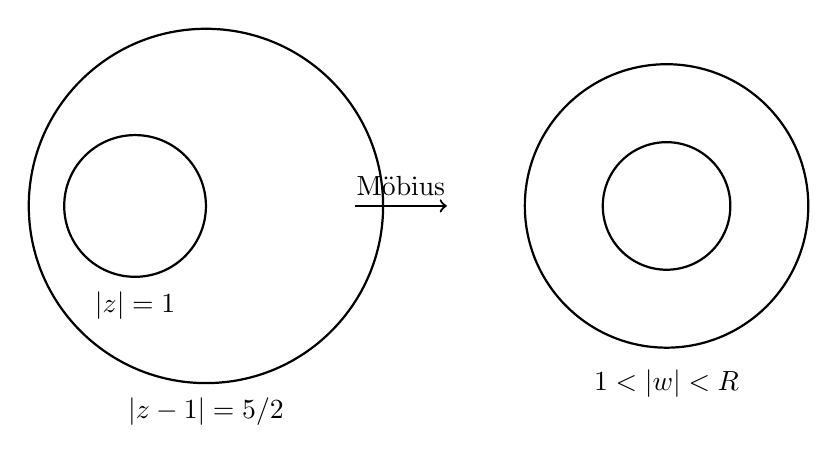
\begin{tikzpicture}[scale=0.9]
  \begin{scope}[xshift=-3.5cm]
    \draw[thick] (0,0) circle (1.0);
    \draw[thick] (1.0,0) circle (2.5);
    \node at (0,-1.4) {$|z|=1$};
    \node at (1.0,-2.9) {$|z-1|=5/2$};
  \end{scope}
  \draw[->,thick] (-0.4,0)--(0.9,0) node[midway,above] {Möbius};
  \begin{scope}[xshift=4.0cm]
    \draw[thick] (0,0) circle (2.0);
    \draw[thick] (0,0) circle (0.9);
    \node at (0,-2.5) {$1<|w|<R$};
  \end{scope}
\end{tikzpicture}
\caption{A suitable Möbius map sends the two disjoint circles in their coaxal family to concentric circles. The region between them therefore becomes a round annulus $1<|w|<R$.}
\label{fig:cp-iv-0123-coaxal-circles-to-annulus}
\end{figure}


\begin{solution}
\emph{(i)} The maps $\phi_{a,\lambda}$ send $\mathbb D$ to itself and are bijective with inverse $\phi_{-\,\lambda a,\ \overline{\lambda}}$.
Conversely, let $f$ be an automorphism of $\mathbb D$ and set $a=f^{-1}(0)$. Then
$\psi(z)=\dfrac{z-a}{1-\overline{a}z}$ maps $a\mapsto0$, so $g=f\circ\psi^{-1}$ is an automorphism with $g(0)=0$.
By Schwarz, $g(z)=\lambda z$ with $|\lambda|=1$, hence $f(z)=\lambda\,\dfrac{z-a}{1-\overline{a}z}$.

\medskip
\emph{(ii)} The two circles are disjoint and nested. Their coaxal limiting points are the real numbers
\[
p=\frac{2}{7},\qquad q=-\frac{2}{3},
\]
the two solutions of $|x|=\tfrac{1}{2.5}|x-1|$ on $\mathbb R$.
Then
\[
F(z)=\frac{z-p}{z-q}
\]
maps $\{|z|=1\}$ and $\{|z-1|=5/2\}$ to concentric circles $|w|=\rho_1$ and $|w|=\rho_2$ (Apollonius property).
Consequently the region between them maps to the annulus $\{\min(\rho_1,\rho_2)<|w|<\max(\rho_1,\rho_2)\}$.
Rescale to unit inner radius by $G(z)=F(z)/\rho_{\mathrm{inner}}$, obtaining
\[
G:\quad \{1<|w|<R\},\qquad R=\rho_{\mathrm{outer}}/\rho_{\mathrm{inner}}.
\]
(Any equivalent choice obtained by post/pre-composing with disk automorphisms is acceptable.)

\medskip
\emph{(iii)} Let $S_h=\{z:0<\Im z<h\}$. The map
\[
W(z)=\exp\!\Big(\tfrac{2\pi}{h}\,z\Big)
\]
is a conformal bijection $S_h\to \{1<|w|<e^{2\pi}\}$, since $|W(z)|=\exp\!\big(\tfrac{2\pi}{h}\Im z\big)\in(1,e^{2\pi})$.
This cannot be the restriction of a Möbius map: a Möbius map sends parallel boundary lines of a strip to two lines or to two circles meeting at one point, whereas the annulus is bounded by two \emph{concentric} circles (which do not meet).
\end{solution}

\begin{problem}[CP-IV-0124]
\label{prob:cp-iv-0124}
Temperature in a right half–plane with a removed disk

The domain $D$ consists of the right-hand half plane $x>0$ with the circle $|z-a|=b$, $0<b<a$, and its interior removed.
	Find the temperature $u(x,y)$ in steady heat flow if $u=0$ on the $y$ axis, $u=1$ on $|z-a|=b$, and $u\to0$ at infinity.

	\medskip
	\noindent\textit{Hint:} Show that the mapping $\displaystyle \zeta=\frac{z-\alpha}{z+\alpha}$, with $\alpha$ real and positive,
	takes $D$ onto an annular region with the imaginary axis mapping to $|\zeta|=1$ and show that, if $\alpha^{2}=a^{2}-b^{2}$, then the image of $D$ is a concentric circular annulus.

	\bigskip\hrule\bigskip

	Consider the real-parameter Möbius map
	\[
	\zeta=\zeta(z)=\frac{z-\alpha}{z+\alpha}, \qquad \alpha>0.
	\]

	For $z=iy$ we have
	\[
	\left|\frac{iy-\alpha}{iy+\alpha}\right|=1 \quad\text{(numerator and denominator are conjugates),}
	\]
	so the $y$–axis maps to the unit circle $|\zeta|=1$.

	\paragraph{Image of the circle $\boldsymbol{|z-a|=b}$.}
	Write $z=a+be^{i\theta}$ and compute
	\[
	|\zeta|^{2}
	=\frac{|a-\alpha+be^{i\theta}|^{2}}{|a+\alpha+be^{i\theta}|^{2}}
	=\frac{A+B\cos\theta}{C+D\cos\theta},
	\]
	where
	\[
	A=(a-\alpha)^{2}+b^{2}, \qquad B=2b(a-\alpha), \qquad
	C=(a+\alpha)^{2}+b^{2}, \qquad D=2b(a+\alpha).
	\]
	For $|\zeta|$ to be constant on the circle (i.e. the image is a circle \emph{centered at the origin}),
	the $\cos\theta$–dependence must drop out:
	\[
	\frac{A+B\cos\theta}{\,C+D\cos\theta\,}\equiv\frac{A}{C}
	\quad\Longleftrightarrow\quad AD=BC.
	\]
	We now verify that
	\[
	AD-BC
	=2b\Big[(a+\alpha)((a-\alpha)^{2}+b^{2})-(a-\alpha)((a+\alpha)^{2}+b^{2})\Big]
	=4b\alpha\,(\alpha^{2}+b^{2}-a^{2}).
	\]
	Thus $AD=BC$ is equivalent to
	\[
	\boxed{\ \alpha^{2}=a^{2}-b^{2}\ }.
	\]
	With this choice (note $a>b>0\Rightarrow \alpha>0$), the ratio becomes \emph{constant}:
	\[
	|\zeta|^{2}=\frac{A}{C}
	=\frac{(a-\alpha)^{2}+b^{2}}{(a+\alpha)^{2}+b^{2}}
	=\frac{2a(a-\alpha)}{2a(a+\alpha)}
	=\frac{a-\alpha}{a+\alpha}.
	\]
	Hence the circle $|z-a|=b$ maps to the circle $|\zeta|=\rho$ with
	\[
	\boxed{\ \rho=\sqrt{\frac{a-\alpha}{a+\alpha}}\in(0,1). \ }
	\]

	Therefore, for $\alpha=\sqrt{a^{2}-b^{2}}$, the map $z\mapsto\zeta$ sends the domain $D$
	(right half–plane with the closed disk $\{|z-a|\le b\}$ removed) onto the concentric circular \emph{annulus}
	\[
	\mathcal A=\{\ \rho<|\zeta|<1\ \}.
	\]
	The boundary pieces correspond as follows:
	\[
	\{x=0\}\ \longmapsto\ |\zeta|=1,
	\qquad
	\{|z-a|=b\}\ \longmapsto\ |\zeta|=\rho.
	\]

	\bigskip\hrule\bigskip

	Let $U(\zeta)$ denote the temperature in the $\zeta$–plane. Harmonicity is preserved by conformal maps, so
	$U$ is harmonic on $\mathcal A$ and the boundary data become
	\[
	U=0 \ \ \text{on}\ \ |\zeta|=1,
	\qquad
	U=1 \ \ \text{on}\ \ |\zeta|=\rho.
	\]
	By rotational symmetry, $U$ depends only on $r=|\zeta|$. The general radial harmonic function on an annulus is
	$A\log r + B$. Imposing the boundary values gives
	\[
	U(r)=\frac{\log(1/r)}{\log(1/\rho)}
	=\frac{-\log r}{-\log \rho}
	=\frac{\log r}{\log \rho}
	\quad\text{for}\quad \rho<r<1.
	\]
	(Any of the three displayed forms is correct; we will use the first one momentarily.)

	\bigskip\hrule\bigskip

	The physical temperature is $u(z)=U(\zeta(z))$ with $r=|\zeta(z)|=\left|\frac{z-\alpha}{z+\alpha}\right|$.
	Hence
	\[
	u(z)
	=U\!\left(\left|\frac{z-\alpha}{z+\alpha}\right|\right)
	=\frac{\displaystyle \log\!\left(\frac{1}{\left|\frac{z-\alpha}{z+\alpha}\right|}\right)}
	{\displaystyle \log\!\left(\frac{1}{\rho}\right)}
	=\frac{\displaystyle \log\left|\frac{z+\alpha}{z-\alpha}\right|}
	{\displaystyle \log\!\left(\frac{1}{\rho}\right)}.
	\]
	Since $\displaystyle \rho=\sqrt{\frac{a-\alpha}{a+\alpha}}$ we have
	\[
	\log\!\left(\frac{1}{\rho}\right)
	=\frac{1}{2}\,\log\!\left(\frac{a+\alpha}{a-\alpha}\right).
	\]
	Therefore a convenient explicit form is
	\[
	\boxed{\quad
		u(z)
		=\frac{2\,\log\!\left|\dfrac{z+\alpha}{z-\alpha}\right|}
		{\log\!\left(\dfrac{a+\alpha}{a-\alpha}\right)},
		\qquad
		\alpha=\sqrt{a^{2}-b^{2}}.
		\quad}
	\]

	\bigskip

		\par\noindent\textbullet\quad \textbf{On the $y$--axis $x=0$:} for $z=iy$ we have $\left|\dfrac{z-\alpha}{z+\alpha}\right|=1$,
		so the numerator $\log\left|\dfrac{z+\alpha}{z-\alpha}\right|=0$ and hence $u=0$.
		\par\noindent\textbullet\quad \textbf{On the circle $|z-a|=b$:} by construction $|\zeta|=\rho$, i.e.
		$\left|\dfrac{z-\alpha}{z+\alpha}\right|=\rho$, so
		$\log\left|\dfrac{z+\alpha}{z-\alpha}\right|=\log\!\left(\dfrac{1}{\rho}\right)$
		and the fraction evaluates to $u=1$.
		\par\noindent\textbullet\quad \textbf{At infinity:} as $|z|\to\infty$, $\left|\dfrac{z+\alpha}{z-\alpha}\right|\to 1$,
		so the numerator $\to 0$ and $u(z)\to 0$.

	\bigskip\hrule\bigskip

	With $\alpha=\sqrt{a^{2}-b^{2}}$ and $\displaystyle \rho=\sqrt{\frac{a-\alpha}{a+\alpha}}$,
	the Möbius map $\displaystyle \zeta=\frac{z-\alpha}{z+\alpha}$ carries
	$D$ onto the annulus $\{\rho<|\zeta|<1\}$.
	The unique harmonic function with $U=1$ on $|\zeta|=\rho$ and $U=0$ on $|\zeta|=1$
	is $U(r)=\log(1/r)/\log(1/\rho)$, and hence
	\[
	u(z)=\frac{2\,\log\!\left|\dfrac{z+\alpha}{z-\alpha}\right|}
	{\log\!\left(\dfrac{a+\alpha}{a-\alpha}\right)}.
	\]
	This $u$ satisfies all the prescribed boundary conditions and $u(z)\to 0$ as $|z|\to\infty$.

\textbf{Background:} entire, odd; period $2\pi i$. \quad
\textbf{Zeros:} $z=i\pi k$; \textbf{poles:} none.\\
\textbf{Decomposition: } $w=u+iv=\sinh x\cos y + i\,\cosh x\sin y$.\\
\textbf{Vertical lines } $x=\text{const}$: $\left(\frac{u}{\sinh x}\right)^2+\left(\frac{v}{\cosh x}\right)^2=1$ (ellipses, foci $\pm i$).\\
\textbf{Horizontal lines } $y=\text{const}$: $\left(\frac{u}{\cos y}\right)^2-\left(\frac{v}{\sin y}\right)^2=-1$ (hyperbolas, foci $\pm i$).\\
\textbf{Strip mapping:}
\[
\boxed{\,\sinh:\ \{|\Im z|<\tfrac{\pi}{2}\}\ \xrightarrow{\ 1\text{--}1\ }\ \mathbb C\setminus i\big((-\infty,-1]\cup[1,\infty)\big)\,}
\]
Boundaries $y=\pm\frac{\pi}{2}$ map to imaginary rays $\pm i[1,\infty)$.

\bigskip\hrule\bigskip

\textbf{Background:} entire, even; period $2\pi i$. \quad
\textbf{Zeros:} $z=i\pi(k+\frac12)$; \textbf{poles:} none.\\
\textbf{Decomposition: } $w=u+iv=\cosh x\cos y + i\,\sinh x\sin y$.\\
\textbf{Vertical lines } $x=\text{const}$: $\left(\frac{u}{\cosh x}\right)^2+\left(\frac{v}{\sinh x}\right)^2=1$ (ellipses, foci $\pm1$).\\
\textbf{Horizontal lines } $y=\text{const}$: $\left(\frac{u}{\cos y}\right)^2-\left(\frac{v}{\sin y}\right)^2=1$ (hyperbolas, foci $\pm1$).\\
\textbf{Strip mapping:}
\[
\boxed{\,\cosh:\ \{|\Im z|<\pi\}\ \xrightarrow{\ 2\text{--}1\ }\ \mathbb C\setminus\big((-\infty,-1]\cup[1,\infty)\big)\,}
\]
On the half-strip $0<|\Im z|<\pi$, the map is 1--1 onto the slit plane.

\bigskip\hrule\bigskip

\textbf{Background:} meromorphic, odd; period $i\pi$. \quad
\textbf{Zeros:} $z=i\pi k$; \textbf{poles:} $z=i\pi(k+\tfrac12)$.\\
\textbf{Strip $\to$ disk:}
\[
\boxed{\,\tanh:\ \{|\Im z|<\tfrac{\pi}{2}\}\ \xrightarrow{\ 1\text{--}1\ }\ \mathbb D\,}
\]
Real line maps to $(-1,1)$; as $|\Im z|\to\pi/2$, $|\tanh z|\to1$.

\bigskip\hrule\bigskip

\textbf{Background:} meromorphic, odd; period $i\pi$. \quad
\textbf{Zeros:} $z=i\pi(k+\tfrac12)$; \textbf{poles:} $z=i\pi k$.\\
\textbf{Strip $\to$ exterior disk:}
\[
\boxed{\,\coth:\ \{|\Im z|<\tfrac{\pi}{2}\}\setminus\{0\}\ \xrightarrow{\ 1\text{--}1\ }\ \{\,|w|>1\,\}\,}
\]
Real line maps to $(-\infty,-1)\cup(1,\infty)$; $|\Im z|\to\pi/2$ gives $|w|\to1^+$.

Throughout, write $z=x+iy$, $x,y\in\mathbb R$, and $w=u+iv$ for the image.
Recall the basic identities
\[
\cosh z=\frac{e^{z}+e^{-z}}{2},\qquad
\sinh z=\frac{e^{z}-e^{-z}}{2},\qquad
\tanh z=\frac{\sinh z}{\cosh z},\qquad
\coth z=\frac{\cosh z}{\sinh z}.
\]
We use the principal branch of the logarithm $\log$ on $\mathbb C\setminus(-\infty,0]$, and principal square roots $\sqrt{\cdot}$ with branch cut on $(-\infty,0]$ unless stated otherwise.

\bigskip\hrule\bigskip

 \mbox{}\\[2pt]
$\sinh$ is an \emph{entire}, \emph{odd} function, with imaginary-periodicity:
\[
\sinh(-z)=-\sinh z,\qquad \sinh(z+2\pi i)=\sinh z.
\]
Zeros occur at $z_k=i\pi k$ for $k\in\mathbb Z$ (all simple). No poles.

\medskip

 \mbox{}\\[2pt]
With $z=x+iy$,
\[
\sinh z=\sinh x\cos y\ +\ i\,\cosh x\sin y \quad\Rightarrow\quad
u=\sinh x\cos y,\ \ v=\cosh x\sin y.
\]
From this, one obtains orthogonal families of confocal conics:
\begin{align*}
	x=\text{const}&:\quad \left(\frac{u}{\sinh x}\right)^{2}+\left(\frac{v}{\cosh x}\right)^{2}=1
	&&\text{(ellipses, foci at $\pm i$)},\\[2pt]
	y=\text{const}&:\quad \left(\frac{u}{\cos y}\right)^{2}-\left(\frac{v}{\sin y}\right)^{2}=-1
	&&\text{(hyperbolas, foci at $\pm i$)}.
\end{align*}
Real and imaginary axes map as:
\[
y=0:\ w=\sinh x\in\mathbb R\ \text{(onto $\mathbb R$)},\qquad
x=0:\ w=i\sin y\ \text{(onto the segment $i[-1,1]$)}.
\]

\medskip

 \mbox{}\\[2pt]
$\sinh'(z)=\cosh z$, and $\cosh z\neq 0$ on the strip $|\Im z|<\tfrac{\pi}{2}$; hence $\sinh$ is conformal there.

\medskip

 \mbox{}\\[2pt]
\[
\boxed{\
	\sinh:\ \{\,|\Im z|<\tfrac{\pi}{2}\,\}\ \xrightarrow[\ \text{biholomorphism}\ ]{}\
	\mathbb C\setminus i\big((-\infty,-1]\cup[1,\infty)\big)\ .
}\]
\emph{Explanation.} The boundary lines $y=\pm\frac{\pi}{2}$ map to the imaginary rays $\pm i[1,\infty)$
(via $v=\cosh x\,\sin y$ with $\sin(\pm\pi/2)=\pm1$ and $u=\sinh x\cos(\pm\pi/2)=0$), while the interior maps injectively since $\cosh z\neq0$ and periodicity in the imaginary direction has period $2\pi$, not $\pi$.

\medskip

 \mbox{}\\[2pt]
A principal inverse on the slit domain is
\[
\operatorname{arsinh} w=\log\!\big(w+\sqrt{w^{2}+1}\big),
\]
with branch cuts along $i(-\infty,-1]\cup i[1,\infty)$ so that $\Im(\operatorname{arsinh} w)\in(-\tfrac{\pi}{2},\tfrac{\pi}{2})$.

\medskip

 \mbox{}\\[2pt]
\[
\cosh^{2}z-\sinh^{2}z=1,\qquad
\sinh(z+\zeta)=\sinh z\,\cosh\zeta+\cosh z\,\sinh\zeta.
\]

\bigskip\hrule\bigskip

 \mbox{}\\[2pt]
$\cosh$ is \emph{entire}, \emph{even}, and $2\pi i$-periodic:
\[
\cosh(-z)=\cosh z,\qquad \cosh(z+2\pi i)=\cosh z.
\]
Zeros at $z=i\pi\big(k+\tfrac12\big)$, all simple. No poles.

\medskip

 \mbox{}\\[2pt]
With $z=x+iy$,
\[
\cosh z=\cosh x\cos y\ +\ i\,\sinh x\sin y \quad\Rightarrow\quad
u=\cosh x\cos y,\ \ v=\sinh x\sin y.
\]
Again one gets confocal conics:
\begin{align*}
	x=\text{const}&:\quad \left(\frac{u}{\cosh x}\right)^{2}+\left(\frac{v}{\sinh x}\right)^{2}=1
	&&\text{(ellipses, foci at $\pm1$)},\\[2pt]
	y=\text{const}&:\quad \left(\frac{u}{\cos y}\right)^{2}-\left(\frac{v}{\sin y}\right)^{2}=1
	&&\text{(hyperbolas, foci at $\pm1$)}.
\end{align*}
On the axes,
\[
y=0:\ w=\cosh x\in[1,\infty),\qquad
x=0:\ w=\cos y\in[-1,1].
\]

\medskip

 \mbox{}\\[2pt]
$\cosh'(z)=\sinh z$, which vanishes at $z=i\pi k$. Thus $\cosh$ fails to be injective across lines $y=k\pi$, but is injective on any strip avoiding these lines (e.g.\ $0<\Im z<\pi$).

\medskip

 \mbox{}\\[2pt]
\[
\boxed{\
	\cosh:\ \{\,0<\Im z<\pi\,\}\ \xrightarrow[\ \text{biholomorphism}\ ]{}\
	\mathbb C\setminus\big((-\infty,-1]\cup[1,\infty)\big)\ .
}\]
\emph{Explanation.} The midline $y=0$ maps to $[1,\infty)$; the top boundary $y=\pi$ maps to $(-\infty,-1]$; injectivity holds on $0<\Im z<\pi$ since there $\sinh z\neq0$.

\medskip

 \mbox{}\\[2pt]
\[
\operatorname{arcosh} w=\log\!\Big(w+\sqrt{w-1}\,\sqrt{w+1}\Big),
\]
with branch cuts along $(-\infty,-1]\cup[1,\infty)$ so that $\Re(\operatorname{arcosh} w)\ge0$ and $0<\Im(\operatorname{arcosh} w)<\pi$ on the principal sheet.

\medskip

 \mbox{}\\[2pt]
\[
\cosh(z+\zeta)=\cosh z\,\cosh\zeta+\sinh z\,\sinh\zeta,\qquad
\cosh z=1+2\sinh^{2}\!\frac{z}{2}.
\]

\bigskip\hrule\bigskip

 \mbox{}\\[2pt]
$\tanh$ is \emph{meromorphic}, \emph{odd}, and $i\pi$-periodic:
\[
\tanh(-z)=-\tanh z,\qquad \tanh(z+i\pi)=\tanh z.
\]
Zeros at $z=i\pi k$; poles (simple) at $z=i\pi\big(k+\tfrac12\big)$.

\medskip

 \mbox{}\\[2pt]
\[
\boxed{\
	\tanh:\ \{\,|\Im z|<\tfrac{\pi}{2}\,\}\ \xrightarrow[\ \text{biholomorphism}\ ]{}\ \mathbb D\ .
}\]
\emph{Boundary correspondence.} The real axis $y=0$ maps bijectively onto $(-1,1)$ (strictly increasing).
As $y\to\pm\frac{\pi}{2}$, $|\tanh(x+iy)|\to1$ uniformly in $x$; hence the horizontal boundaries map to $\partial\mathbb D$.

\medskip

 \mbox{}\\[2pt]
\[
\operatorname{artanh} w=\frac{1}{2}\log\!\left(\frac{1+w}{1-w}\right),
\qquad |w|<1,
\]
which maps $\mathbb D$ conformally onto $\{|\Im z|<\tfrac{\pi}{2}\}$.

\medskip

 \mbox{}\\[2pt]
\[
(\tanh z)'=\operatorname{sech}^{2}\!z,\qquad
\left|\tanh'(z)\right|=\frac{1}{|\cosh z|^{2}}
\]
and conjugating by a disk automorphism shows $\tanh$ is extremal for the disk-strip version of Schwarz--Pick.

\medskip

 \mbox{}\\[2pt]
Lines $x=\text{const}$ and $y=\text{const}$ in the strip map to orthogonal circle arcs inside $\mathbb D$ meeting $\partial\mathbb D$ orthogonally (images of preimages under the conformal equivalence with the half-plane followed by a Cayley map).

\bigskip\hrule\bigskip

 \mbox{}\\[2pt]
$\coth$ is \emph{meromorphic}, \emph{odd}, and $i\pi$-periodic:
\[
\coth(-z)=-\coth z,\qquad \coth(z+i\pi)=\coth z.
\]
Poles (simple) at $z=i\pi k$; zeros (simple) at $z=i\pi\big(k+\tfrac12\big)$.

\medskip

 \mbox{}\\[2pt]
\[
\boxed{\
	\coth:\ \{\,|\Im z|<\tfrac{\pi}{2}\,\}\setminus\{0\}\ \xrightarrow[\ \text{biholomorphism}\ ]{}\ \{\,|w|>1\,\}\ .
}\]
\emph{Boundary correspondence.} The real axis (excluding $0$) maps to the rays $(-\infty,-1)\cup(1,\infty)$.
As $y\to\pm\frac{\pi}{2}$, $|\coth(x+iy)|\to1^{+}$; thus horizontal boundaries map to the unit circle from the \emph{exterior} side.

\medskip

 \mbox{}\\[2pt]
\[
\operatorname{arcoth} w=\frac{1}{2}\log\!\left(\frac{w+1}{w-1}\right),\qquad |w|>1,
\]
with the standard logarithm branch so that $\Im(\operatorname{arcoth} w)\in(-\tfrac{\pi}{2},\tfrac{\pi}{2})$.

\medskip

 \mbox{}\\[2pt]
\[
\coth z=\tanh\!\left(z+\tfrac{i\pi}{2}\right),
\]
so the exterior-disk picture is just the disk picture shifted vertically by $i\pi/2$ and inverted via $w\mapsto 1/w$.

\bigskip\hrule\bigskip

 \mbox{}\\[2pt]
\[
\operatorname{arsinh} w=\log\!\big(w+\sqrt{w^{2}+1}\big),\qquad
\operatorname{arcosh} w=\log\!\big(w+\sqrt{w-1}\,\sqrt{w+1}\big),
\]
\[
\operatorname{artanh} w=\frac12\log\!\left(\frac{1+w}{1-w}\right),\qquad
\operatorname{arcoth} w=\frac12\log\!\left(\frac{w+1}{w-1}\right).
\]
Branch cuts are chosen to match the canonical target domains described above.

\medskip

 \mbox{}\\[2pt]
Using the Cayley map $C(\zeta)=\frac{1+\zeta}{1-\zeta}$ and its inverse $C^{-1}(w)=\frac{w-1}{w+1}$,
\[
\tanh z=\ C^{-1}\!\left(e^{2z}\right),\qquad
\coth z=\ C^{-1}\!\left(e^{2z}\right)^{-1},\qquad
\sinh z=\frac{e^{z}-e^{-z}}{2},\quad \cosh z=\frac{e^{z}+e^{-z}}{2}.
\]
Thus strip $\leftrightarrow$ disk/exterior-disk mappings for $\tanh$ and $\coth$ are just the exponential’s strip-to-sector equivalences composed with a Cayley map.

\medskip

 \mbox{}\\[2pt]
As $x\to\pm\infty$ with $y$ fixed, $\sinh z\sim \frac12 e^{x}e^{iy}$ and $\cosh z\sim \frac12 e^{x}e^{iy}$; hence horizontal lines map to asymptotically radial curves. For $\tanh$ and $\coth$, $|\tanh(x+iy)|\to 1$ and $|\coth(x+iy)|\to 1$ exponentially in $|x|$ (uniform in $y$ within the strip height).

\medskip

 \mbox{}\\[2pt]
$\sinh'(z)=\cosh z$ vanishes along $y=\frac{\pi}{2}+\pi\mathbb Z$; $\cosh'(z)=\sinh z$ vanishes along $y=\pi\mathbb Z$.
Therefore, the natural injectivity strips are $|\Im z|<\tfrac{\pi}{2}$ for $\sinh$ and $0<\Im z<\pi$ for $\cosh$.
For $\tanh$ and $\coth$, poles on the horizontal boundaries determine the natural strip height $\pi$.

\bigskip\hrule\bigskip

\[
\boxed{\
	\sinh:\ \{\,|\Im z|<\tfrac{\pi}{2}\,\}\ \longrightarrow\
	\mathbb C\setminus i\big((-\infty,-1]\cup[1,\infty)\big)\ \ \text{(biholomorphism)}\ .
}\]
\[
\boxed{\
	\cosh:\ \{\,0<\Im z<\pi\,\}\ \longrightarrow\
	\mathbb C\setminus\big((-\infty,-1]\cup[1,\infty)\big)\ \ \text{(biholomorphism)}\ .
}\]
\[
\boxed{\
	\tanh:\ \{\,|\Im z|<\tfrac{\pi}{2}\,\}\ \longrightarrow\ \mathbb D\ \ \text{(biholomorphism)}\ .
}\]
\[
\boxed{\
	\coth:\ \{\,|\Im z|<\tfrac{\pi}{2}\,\}\setminus\{0\}\ \longrightarrow\ \{\,|w|>1\,\}\ \ \text{(biholomorphism)}\ .
}\]

\medskip

If $\sinh z_{1}=\sinh z_{2}$ then $e^{z_{1}}-e^{-z_{1}}=e^{z_{2}}-e^{-z_{2}}$.
Rearranging gives $\{e^{z_{1}},e^{-z_{1}}\}=\{e^{z_{2}},e^{-z_{2}}\}$.
Taking logs in the horizontal strip $|\Im z|<\pi/2$ (where the exponential is injective modulo $2\pi i$) forces $z_{1}=z_{2}$.

Set $z=x\pm i\pi/2$. Then $\sinh z=\sinh x\cdot 0 \ \pm i\,\cosh x$, so the boundaries map to $\pm i[1,\infty)$; the interior cannot reach those rays by the open mapping theorem and the maximum modulus principle applied to $1/(\sinh z\mp i)$.

  apply to $\cosh$ (use $\sinh$ zeros to avoid critical lines) and to $\tanh,\coth$ using the representation via exponentials and the Cayley transform.

	\par\noindent\textbullet\quad \textbf{Cayley (disk $\leftrightarrow$ right half-plane).}\\[2pt]
	\[
	\boxed{\,w=\frac{1+z}{1-z}\,}\qquad\text{inverse:}\quad z=\frac{w-1}{w+1}.
	\]

	\par\noindent\textbullet\quad \textbf{Half-plane $\to$ half-plane (three-point normalization).}\\[2pt]
	\[
	\boxed{\,w=\frac{(z-a)(c-b)}{(z-b)(c-a)}\,}.
	\]

	\par\noindent\textbullet\quad \textbf{Disk automorphisms.}\\[2pt]
	\[
	\boxed{\,\phi_{a,\theta}(z)=e^{i\theta}\frac{z-a}{1-\bar a z}\,},\qquad |a|<1.
	\]

	\par\noindent\textbullet\quad \textbf{Strip $|\Im z|<h/2$ $\to$ right half-plane.}\\[2pt]
	\[
	\boxed{\,w=\exp\!\left(\frac{\pi z}{h}\right)\,}.
	\]

	\par\noindent\textbullet\quad \textbf{Strip $|\Im z|<h/2$ $\to$ unit disk.}\\[2pt]
	\[
	\boxed{\,\zeta=\frac{e^{\pi z/h}-1}{\,e^{\pi z/h}+1\,}\,}.
	\]

	\par\noindent\textbullet\quad \textbf{Strip $\to$ strip (height scaling).}\\[2pt]
	\[
	\boxed{\,z\mapsto \frac{h_2}{h_1}\,z\,}.
	\]

	\par\noindent\textbullet\quad \textbf{Band $a<\Im z<b$ $\to$ centered strip.}\\[2pt]
	\[
	\boxed{\,z\mapsto \frac{\pi}{b-a}\!\left(z-i\frac{a+b}{2}\right)\,}.
	\]

	\par\noindent\textbullet\quad \textbf{Sector $\{0<\arg z<\alpha\}$ $\to$ upper half-plane.}\\[2pt]
	\[
	\boxed{\,w=z^{\pi/\alpha}\,}\ \ \text{(principal branch)}.
	\]

	\par\noindent\textbullet\quad \textbf{Wedge $\to$ disk.}\\[2pt]
	Compose item (8) with Cayley (item 1).

	\par\noindent\textbullet\quad \textbf{Upper half-plane $\to$ disk (prescribed triple).}\\[2pt]
	\[
	\boxed{\,\Phi(z)=\frac{(z-a)}{(z-\bar a)}\cdot \frac{(b-\bar a)}{(b-a)}\,}.
	\]

	\par\noindent\textbullet\quad \textbf{Annulus $r<|z|<1$ $\leftrightarrow$ strip.}\\[2pt]
	\[
	\boxed{\,w=\log z\,}\quad\text{maps to }\ \log r<\Re w<0.
	\]

	\par\noindent\textbullet\quad \textbf{Annulus $\to$ disk.}\\[2pt]
	Use $w=\log z$ then item (5).

	\par\noindent\textbullet\quad \textbf{Half-plane minus disk $\to$ annulus.}\\[2pt]
	\[
	\boxed{\,\zeta=\frac{z-\alpha}{z+\alpha}\,},\qquad \alpha^{2}=a^{2}-b^{2}.
	\]

	\par\noindent\textbullet\quad \textbf{Disk with off-center hole $\to$ annulus.}\\[2pt]
	Center via $\phi_a$ (item 3), then items (11)–(12).

	\par\noindent\textbullet\quad \textbf{Punctured plane $\leftrightarrow$ cylinder.}\\[2pt]
	\[
	\boxed{\,w=\log z\,}\quad(\text{period }2\pi i).
	\]

	\par\noindent\textbullet\quad \textbf{Strip $\to$ punctured plane.}\\[2pt]
	\[
	\boxed{\,z\mapsto e^{z}\,}.
	\]

	\par\noindent\textbullet\quad \textbf{Ray-slit plane $\mathbb C\setminus[0,\infty)$ $\to$ half-plane.}\\[2pt]
	\[
	\boxed{\,w=\sqrt{z}\,}\ \ \text{(choose branch)}.
	\]

	\par\noindent\textbullet\quad \textbf{Segment-slit plane $\mathbb C\setminus[a,b]$ $\to$ half-plane.}\\[2pt]
	\[
	\boxed{\,w=\sqrt{\frac{z-a}{\,z-b\,}}\,}.
	\]

	\par\noindent\textbullet\quad \textbf{Exterior of $[-1,1]$ $\leftrightarrow$ exterior unit circle (Joukowski).}\\[2pt]
	\[
	\boxed{\,w=z+\frac{1}{z}\,},\qquad
	z=\frac{w\pm\sqrt{w^{2}-4}}{2}.
	\]

	\par\noindent\textbullet\quad \textbf{Exterior of ellipse $\leftrightarrow$ exterior unit circle.}\\[2pt]
	\[
	\boxed{\,w=\tfrac12\!\left(c z+\frac{1}{c z}\right)\,}\quad(\text{$c$ from axes}).
	\]

	\par\noindent\textbullet\quad \textbf{Right half-plane $\to$ vertical strip.}\\[2pt]
	\[
	\boxed{\,z\mapsto \frac{1}{\pi}\log\frac{z-1}{\,z+1\,}\,}.
	\]

	\par\noindent\textbullet\quad \textbf{Upper half-plane $\to$ rectangle (SC/elliptic).}\\[2pt]
	\[
	\boxed{\,\zeta=\int^z \frac{dt}{\sqrt{(t-a)(t-b)(t-c)(t-d)}}\,}.
	\]

	\par\noindent\textbullet\quad \textbf{Rectangle $\to$ disk (Jacobi sn).}\\[2pt]
	\[
	\boxed{\,\zeta=\operatorname{sn}\!\left(\frac{K(k)}{L}\,z;\,k\right)\,}.
	\]

	\par\noindent\textbullet\quad \textbf{Half-disk $\leftrightarrow$ half-plane.}\\[2pt]
	Restriction of Cayley (item 1) and inverse.

	\par\noindent\textbullet\quad \textbf{Lens (intersection of two disks) $\to$ disk.}\\[2pt]
	Möbius normalizes the circles; then a power map; then Cayley.

	\par\noindent\textbullet\quad \textbf{Half-strip $\{x>0,\ 0<\Im z<h\}$ $\to$ half-disk.}\\[2pt]
	\[
	\boxed{\,\exp(\pi z/h)\,}\ \ \text{then power, then Cayley}.
	\]

	\par\noindent\textbullet\quad \textbf{Polygon $\to$ half-plane (Schwarz--Christoffel).}\\[2pt]
	\[
	\boxed{\,\Phi'(z)=C\prod_k (z-z_k)^{\alpha_k-1}\,},\qquad \sum\alpha_k=2.
	\]

	\par\noindent\textbullet\quad \textbf{Upper half-plane $\to$ slit half-plane.}\\[2pt]
	\[
	\boxed{\,w=z+\frac{1}{z}\,}\ \ \text{then a real Möbius adjustment}.
	\]

	\par\noindent\textbullet\quad \textbf{Disk $\to$ disk with boundary arc removed.}\\[2pt]
	Automorphism to put endpoints at $\pm1$, then boundary power $z^\lambda$.

	\par\noindent\textbullet\quad \textbf{Finite Blaschke product (disk $\to$ disk, degree $n$).}\\[2pt]
	\[
	\boxed{\,B(z)=e^{i\theta}\prod_{k=1}^n \frac{z-a_k}{\,1-\bar a_k z\,}\,}.
	\]

 \mbox{}\\[2pt]
\[
w=\frac{1+z}{\,1-z\,}
\quad\text{maps}\quad
\mathbb D=\{|z|<1\}\ \text{onto}\ \{\,\Re w>0\,\},
\qquad
z=\frac{w-1}{\,w+1\,}
\]
is the inverse.

\medskip

 \mbox{}\\[2pt]
Compute
\[
\Re\!\left(\frac{1+z}{\,1-z\,}\right)
=\frac{\,1-|z|^{2}\,}{\,|1-z|^{2}\,}.
\]
Thus $\Re w>0$ for $|z|<1$, and $\Re w=0$ for $|z|=1$ (except $z=1$, which maps to $w=\infty$).
Therefore
\[
|z|<1\ \Longleftrightarrow\ \Re w>0,
\qquad
|z|=1\ \Longleftrightarrow\ \Re w=0 .
\]

\medskip

 \mbox{}\\[2pt]
$z=0\mapsto w=1$,
\quad
$z\to1^{-}\mapsto w\to+\infty$,
\quad
and $\partial\mathbb D\setminus\{1\}$ maps to the line $\Re w=0$.\\[2pt]
Circles/lines orthogonal to $\partial\mathbb D$ map to \emph{vertical} lines in the $w$–plane.

\bigskip\hrule\bigskip

 \mbox{}\\[2pt]
Let $L$ be a line or circle, and choose three distinct points $a,b,c\in L$. Define
\[
\Phi(z)=\frac{(z-a)(c-b)}{(z-b)(c-a)}.
\]
Then $\Phi(L)\subset\mathbb R\cup\{\infty\}$, with
\[
\Phi(a)=0,\qquad \Phi(b)=\infty,\qquad \Phi(c)=1,
\]
and the two sides of $L$ map to the half-planes $\Im\Phi(z)\gtrless 0$.

\medskip

 \mbox{}\\[2pt]
Given half-planes $H_1,H_2$ with boundary arcs $L_1,L_2$,
pick ordered boundary triples $a,b,c\in L_1$ and $A,B,C\in L_2$ (same cyclic order).
Then
\[
T(z)=\frac{(z-a)(c-b)}{(z-b)(c-a)}\cdot\frac{(C-A)}{(C-B)}
\]
is a Möbius map sending $L_1\!\to L_2$ with
\[
a\mapsto A,\qquad b\mapsto B,\qquad c\mapsto C,
\]
and taking the chosen side of $H_1$ onto the chosen side of $H_2$.

\medskip

 \mbox{}\\[2pt]
To send $L$ to $\mathbb R$, use $\Phi$ above; then pre/postcompose with an \emph{affine real} map
\[
\xi\longmapsto \alpha\,\xi+\beta,\qquad \alpha>0,
\]
to obtain any target half-plane, e.g.\ $\Re w>0$ or $\Im w>0$.
\end{problem}

% Designed Companion Part IV figure
% Intended for \input{...} beside the matching canonical problem.
\begin{figure}[ht]
\centering
\begin{tikzpicture}[scale=1.05]
  \fill[gray!8] (0,0) circle (2.15);
  \fill[white] (0,0) circle (0.85);
  \draw[thick] (0,0) circle (2.15);
  \draw[thick] (0,0) circle (0.85);
  \draw[dashed] (0,0) circle (1.25);
  \draw[dashed] (0,0) circle (1.65);
  \node[right] at (2.05,0.35) {$U=0$};
  \node[right] at (0.8,-0.35) {$U=1$};
  \node at (0,-2.7) {$U(r)=\dfrac{\log(1/r)}{\log(1/\rho)}$};
\end{tikzpicture}
\caption{After the Möbius normalization, the Dirichlet problem is radial on the annulus. Constant-temperature curves are concentric circles and $U(r)=\log(1/r)/\log(1/\rho)$ interpolates between $1$ at $r=\rho$ and $0$ at $r=1$.}
\label{fig:cp-iv-0124-radial-temperature-annulus}
\end{figure}


\begin{solution}
Set
\[
\alpha=\sqrt{a^2-b^2}>0,
\qquad
\zeta=\frac{z-\alpha}{z+\alpha}.
\]
If \(z=iy\), then numerator and denominator have the same modulus, so
\[
|\zeta|=1.
\]
Thus the \(y\)-axis maps to the outer unit circle.

Now put
\[
z=a+be^{i\theta}.
\]
Then
\[
|\zeta|^2
=
\frac{(a-\alpha)^2+b^2+2b(a-\alpha)\cos\theta}
{(a+\alpha)^2+b^2+2b(a+\alpha)\cos\theta}.
\]
Because
\[
\alpha^2=a^2-b^2,
\]
the ratio is independent of \(\theta\), and
\[
|\zeta|^2
=
\frac{a-\alpha}{a+\alpha}.
\]
Hence
\[
|z-a|=b
\quad\longmapsto\quad
|\zeta|=\rho,
\qquad
\rho=
\sqrt{\frac{a-\alpha}{a+\alpha}}.
\]
Therefore the physical domain is mapped conformally onto
\[
\rho<|\zeta|<1.
\]

The rotationally symmetric harmonic function on this annulus satisfying
\[
U=1\quad(|\zeta|=\rho),
\qquad
U=0\quad(|\zeta|=1)
\]
is
\[
U(\zeta)
=
\frac{\log(1/|\zeta|)}{\log(1/\rho)}.
\]
Pulling back gives
\[
u(z)
=
\frac{\log\left|\dfrac{z+\alpha}{z-\alpha}\right|}
{\log(1/\rho)}.
\]
Since
\[
\log\frac1\rho
=
\frac12
\log\left(\frac{a+\alpha}{a-\alpha}\right),
\]
we obtain
\[
\boxed{
u(z)
=
\frac{
2\log\left|\dfrac{z+\alpha}{z-\alpha}\right|
}{
\log\left(\dfrac{a+\alpha}{a-\alpha}\right)
},
\qquad
\alpha=\sqrt{a^2-b^2}.
}
\]
On the \(y\)-axis the numerator is \(0\); on the removed circle it equals the denominator; and as \(|z|\to\infty\), the logarithm tends to \(0\). Hence all prescribed boundary conditions are satisfied.
\end{solution}


\begin{problem}[CP-IV-0135]
\label{prob:cp-iv-0135}
Temperature in a right half–plane with a removed disk

The domain $D$ consists of the right-hand half plane $x>0$ with the circle $|z-a|=b$, $0<b<a$, and its interior removed.
	Find the temperature $u(x,y)$ in steady heat flow if $u=0$ on the $y$ axis, $u=1$ on $|z-a|=b$, and $u\to0$ at infinity.

	\medskip
	\noindent\textit{Hint:} Show that the mapping $\displaystyle \zeta=\frac{z-\alpha}{z+\alpha}$, with $\alpha$ real and positive,
	takes $D$ onto an annular region with the imaginary axis mapping to $|\zeta|=1$ and show that, if $\alpha^{2}=a^{2}-b^{2}$, then the image of $D$ is a concentric circular annulus.

	\bigskip\hrule\bigskip

	Consider the real-parameter Möbius map
	\[
	\zeta=\zeta(z)=\frac{z-\alpha}{z+\alpha}, \qquad \alpha>0.
	\]

	For $z=iy$ we have
	\[
	\left|\frac{iy-\alpha}{iy+\alpha}\right|=1 \quad\text{(numerator and denominator are conjugates),}
	\]
	so the $y$–axis maps to the unit circle $|\zeta|=1$.

	\paragraph{Image of the circle $\boldsymbol{|z-a|=b}$.}
	Write $z=a+be^{i\theta}$ and compute
	\[
	|\zeta|^{2}
	=\frac{|a-\alpha+be^{i\theta}|^{2}}{|a+\alpha+be^{i\theta}|^{2}}
	=\frac{A+B\cos\theta}{C+D\cos\theta},
	\]
	where
	\[
	A=(a-\alpha)^{2}+b^{2}, \qquad B=2b(a-\alpha), \qquad
	C=(a+\alpha)^{2}+b^{2}, \qquad D=2b(a+\alpha).
	\]
	For $|\zeta|$ to be constant on the circle (i.e. the image is a circle \emph{centered at the origin}),
	the $\cos\theta$–dependence must drop out:
	\[
	\frac{A+B\cos\theta}{\,C+D\cos\theta\,}\equiv\frac{A}{C}
	\quad\Longleftrightarrow\quad AD=BC.
	\]
	We now verify that
	\[
	AD-BC
	=2b\Big[(a+\alpha)((a-\alpha)^{2}+b^{2})-(a-\alpha)((a+\alpha)^{2}+b^{2})\Big]
	=4b\alpha\,(\alpha^{2}+b^{2}-a^{2}).
	\]
	Thus $AD=BC$ is equivalent to
	\[
	\boxed{\ \alpha^{2}=a^{2}-b^{2}\ }.
	\]
	With this choice (note $a>b>0\Rightarrow \alpha>0$), the ratio becomes \emph{constant}:
	\[
	|\zeta|^{2}=\frac{A}{C}
	=\frac{(a-\alpha)^{2}+b^{2}}{(a+\alpha)^{2}+b^{2}}
	=\frac{2a(a-\alpha)}{2a(a+\alpha)}
	=\frac{a-\alpha}{a+\alpha}.
	\]
	Hence the circle $|z-a|=b$ maps to the circle $|\zeta|=\rho$ with
	\[
	\boxed{\ \rho=\sqrt{\frac{a-\alpha}{a+\alpha}}\in(0,1). \ }
	\]

	Therefore, for $\alpha=\sqrt{a^{2}-b^{2}}$, the map $z\mapsto\zeta$ sends the domain $D$
	(right half–plane with the closed disk $\{|z-a|\le b\}$ removed) onto the concentric circular \emph{annulus}
	\[
	\mathcal A=\{\ \rho<|\zeta|<1\ \}.
	\]
	The boundary pieces correspond as follows:
	\[
	\{x=0\}\ \longmapsto\ |\zeta|=1,
	\qquad
	\{|z-a|=b\}\ \longmapsto\ |\zeta|=\rho.
	\]

	\bigskip\hrule\bigskip

	Let $U(\zeta)$ denote the temperature in the $\zeta$–plane. Harmonicity is preserved by conformal maps, so
	$U$ is harmonic on $\mathcal A$ and the boundary data become
	\[
	U=0 \ \ \text{on}\ \ |\zeta|=1,
	\qquad
	U=1 \ \ \text{on}\ \ |\zeta|=\rho.
	\]
	By rotational symmetry, $U$ depends only on $r=|\zeta|$. The general radial harmonic function on an annulus is
	$A\log r + B$. Imposing the boundary values gives
	\[
	U(r)=\frac{\log(1/r)}{\log(1/\rho)}
	=\frac{-\log r}{-\log \rho}
	=\frac{\log r}{\log \rho}
	\quad\text{for}\quad \rho<r<1.
	\]
	(Any of the three displayed forms is correct; we will use the first one momentarily.)

	\bigskip\hrule\bigskip

	The physical temperature is $u(z)=U(\zeta(z))$ with $r=|\zeta(z)|=\left|\frac{z-\alpha}{z+\alpha}\right|$.
	Hence
	\[
	u(z)
	=U\!\left(\left|\frac{z-\alpha}{z+\alpha}\right|\right)
	=\frac{\displaystyle \log\!\left(\frac{1}{\left|\frac{z-\alpha}{z+\alpha}\right|}\right)}
	{\displaystyle \log\!\left(\frac{1}{\rho}\right)}
	=\frac{\displaystyle \log\left|\frac{z+\alpha}{z-\alpha}\right|}
	{\displaystyle \log\!\left(\frac{1}{\rho}\right)}.
	\]
	Since $\displaystyle \rho=\sqrt{\frac{a-\alpha}{a+\alpha}}$ we have
	\[
	\log\!\left(\frac{1}{\rho}\right)
	=\frac{1}{2}\,\log\!\left(\frac{a+\alpha}{a-\alpha}\right).
	\]
	Therefore a convenient explicit form is
	\[
	\boxed{\quad
		u(z)
		=\frac{2\,\log\!\left|\dfrac{z+\alpha}{z-\alpha}\right|}
		{\log\!\left(\dfrac{a+\alpha}{a-\alpha}\right)},
		\qquad
		\alpha=\sqrt{a^{2}-b^{2}}.
		\quad}
	\]

	\bigskip

		\par\noindent\textbullet\quad \textbf{On the $y$--axis $x=0$:} for $z=iy$ we have $\left|\dfrac{z-\alpha}{z+\alpha}\right|=1$,
		so the numerator $\log\left|\dfrac{z+\alpha}{z-\alpha}\right|=0$ and hence $u=0$.
		\par\noindent\textbullet\quad \textbf{On the circle $|z-a|=b$:} by construction $|\zeta|=\rho$, i.e.
		$\left|\dfrac{z-\alpha}{z+\alpha}\right|=\rho$, so
		$\log\left|\dfrac{z+\alpha}{z-\alpha}\right|=\log\!\left(\dfrac{1}{\rho}\right)$
		and the fraction evaluates to $u=1$.
		\par\noindent\textbullet\quad \textbf{At infinity:} as $|z|\to\infty$, $\left|\dfrac{z+\alpha}{z-\alpha}\right|\to 1$,
		so the numerator $\to 0$ and $u(z)\to 0$.

	\bigskip\hrule\bigskip

	With $\alpha=\sqrt{a^{2}-b^{2}}$ and $\displaystyle \rho=\sqrt{\frac{a-\alpha}{a+\alpha}}$,
	the Möbius map $\displaystyle \zeta=\frac{z-\alpha}{z+\alpha}$ carries
	$D$ onto the annulus $\{\rho<|\zeta|<1\}$.
	The unique harmonic function with $U=1$ on $|\zeta|=\rho$ and $U=0$ on $|\zeta|=1$
	is $U(r)=\log(1/r)/\log(1/\rho)$, and hence
	\[
	u(z)=\frac{2\,\log\!\left|\dfrac{z+\alpha}{z-\alpha}\right|}
	{\log\!\left(\dfrac{a+\alpha}{a-\alpha}\right)}.
	\]
	This $u$ satisfies all the prescribed boundary conditions and $u(z)\to 0$ as $|z|\to\infty$.

\textbf{Background:} entire, odd; period $2\pi i$. \quad
\textbf{Zeros:} $z=i\pi k$; \textbf{poles:} none.\\
\textbf{Decomposition: } $w=u+iv=\sinh x\cos y + i\,\cosh x\sin y$.\\
\textbf{Vertical lines } $x=\text{const}$: $\left(\frac{u}{\sinh x}\right)^2+\left(\frac{v}{\cosh x}\right)^2=1$ (ellipses, foci $\pm i$).\\
\textbf{Horizontal lines } $y=\text{const}$: $\left(\frac{u}{\cos y}\right)^2-\left(\frac{v}{\sin y}\right)^2=-1$ (hyperbolas, foci $\pm i$).\\
\textbf{Strip mapping:}
\[
\boxed{\,\sinh:\ \{|\Im z|<\tfrac{\pi}{2}\}\ \xrightarrow{\ 1\text{--}1\ }\ \mathbb C\setminus i\big((-\infty,-1]\cup[1,\infty)\big)\,}
\]
Boundaries $y=\pm\frac{\pi}{2}$ map to imaginary rays $\pm i[1,\infty)$.

\bigskip\hrule\bigskip

\textbf{Background:} entire, even; period $2\pi i$. \quad
\textbf{Zeros:} $z=i\pi(k+\frac12)$; \textbf{poles:} none.\\
\textbf{Decomposition: } $w=u+iv=\cosh x\cos y + i\,\sinh x\sin y$.\\
\textbf{Vertical lines } $x=\text{const}$: $\left(\frac{u}{\cosh x}\right)^2+\left(\frac{v}{\sinh x}\right)^2=1$ (ellipses, foci $\pm1$).\\
\textbf{Horizontal lines } $y=\text{const}$: $\left(\frac{u}{\cos y}\right)^2-\left(\frac{v}{\sin y}\right)^2=1$ (hyperbolas, foci $\pm1$).\\
\textbf{Strip mapping:}
\[
\boxed{\,\cosh:\ \{|\Im z|<\pi\}\ \xrightarrow{\ 2\text{--}1\ }\ \mathbb C\setminus\big((-\infty,-1]\cup[1,\infty)\big)\,}
\]
On the half-strip $0<|\Im z|<\pi$, the map is 1--1 onto the slit plane.

\bigskip\hrule\bigskip

\textbf{Background:} meromorphic, odd; period $i\pi$. \quad
\textbf{Zeros:} $z=i\pi k$; \textbf{poles:} $z=i\pi(k+\tfrac12)$.\\
\textbf{Strip $\to$ disk:}
\[
\boxed{\,\tanh:\ \{|\Im z|<\tfrac{\pi}{2}\}\ \xrightarrow{\ 1\text{--}1\ }\ \mathbb D\,}
\]
Real line maps to $(-1,1)$; as $|\Im z|\to\pi/2$, $|\tanh z|\to1$.

\bigskip\hrule\bigskip

\textbf{Background:} meromorphic, odd; period $i\pi$. \quad
\textbf{Zeros:} $z=i\pi(k+\tfrac12)$; \textbf{poles:} $z=i\pi k$.\\
\textbf{Strip $\to$ exterior disk:}
\[
\boxed{\,\coth:\ \{|\Im z|<\tfrac{\pi}{2}\}\setminus\{0\}\ \xrightarrow{\ 1\text{--}1\ }\ \{\,|w|>1\,\}\,}
\]
Real line maps to $(-\infty,-1)\cup(1,\infty)$; $|\Im z|\to\pi/2$ gives $|w|\to1^+$.

	\par\noindent\textbullet\quad \textbf{Cayley (disk $\leftrightarrow$ right half-plane).}\\[2pt]
	\[
	\boxed{\,w=\frac{1+z}{1-z}\,}\qquad\text{inverse:}\quad z=\frac{w-1}{w+1}.
	\]

	\par\noindent\textbullet\quad \textbf{Half-plane $\to$ half-plane (three-point normalization).}\\[2pt]
	\[
	\boxed{\,w=\frac{(z-a)(c-b)}{(z-b)(c-a)}\,}.
	\]

	\par\noindent\textbullet\quad \textbf{Disk automorphisms.}\\[2pt]
	\[
	\boxed{\,\phi_{a,\theta}(z)=e^{i\theta}\frac{z-a}{1-\bar a z}\,},\qquad |a|<1.
	\]

	\par\noindent\textbullet\quad \textbf{Strip $|\Im z|<h/2$ $\to$ right half-plane.}\\[2pt]
	\[
	\boxed{\,w=\exp\!\left(\frac{\pi z}{h}\right)\,}.
	\]

	\par\noindent\textbullet\quad \textbf{Strip $|\Im z|<h/2$ $\to$ unit disk.}\\[2pt]
	\[
	\boxed{\,\zeta=\frac{e^{\pi z/h}-1}{\,e^{\pi z/h}+1\,}\,}.
	\]

	\par\noindent\textbullet\quad \textbf{Strip $\to$ strip (height scaling).}\\[2pt]
	\[
	\boxed{\,z\mapsto \frac{h_2}{h_1}\,z\,}.
	\]

	\par\noindent\textbullet\quad \textbf{Band $a<\Im z<b$ $\to$ centered strip.}\\[2pt]
	\[
	\boxed{\,z\mapsto \frac{\pi}{b-a}\!\left(z-i\frac{a+b}{2}\right)\,}.
	\]

	\par\noindent\textbullet\quad \textbf{Sector $\{0<\arg z<\alpha\}$ $\to$ upper half-plane.}\\[2pt]
	\[
	\boxed{\,w=z^{\pi/\alpha}\,}\ \ \text{(principal branch)}.
	\]

	\par\noindent\textbullet\quad \textbf{Wedge $\to$ disk.}\\[2pt]
	Compose item (8) with Cayley (item 1).

	\par\noindent\textbullet\quad \textbf{Upper half-plane $\to$ disk (prescribed triple).}\\[2pt]
	\[
	\boxed{\,\Phi(z)=\frac{(z-a)}{(z-\bar a)}\cdot \frac{(b-\bar a)}{(b-a)}\,}.
	\]

	\par\noindent\textbullet\quad \textbf{Annulus $r<|z|<1$ $\leftrightarrow$ strip.}\\[2pt]
	\[
	\boxed{\,w=\log z\,}\quad\text{maps to }\ \log r<\Re w<0.
	\]

	\par\noindent\textbullet\quad \textbf{Annulus $\to$ disk.}\\[2pt]
	Use $w=\log z$ then item (5).

	\par\noindent\textbullet\quad \textbf{Half-plane minus disk $\to$ annulus.}\\[2pt]
	\[
	\boxed{\,\zeta=\frac{z-\alpha}{z+\alpha}\,},\qquad \alpha^{2}=a^{2}-b^{2}.
	\]

	\par\noindent\textbullet\quad \textbf{Disk with off-center hole $\to$ annulus.}\\[2pt]
	Center via $\phi_a$ (item 3), then items (11)–(12).

	\par\noindent\textbullet\quad \textbf{Punctured plane $\leftrightarrow$ cylinder.}\\[2pt]
	\[
	\boxed{\,w=\log z\,}\quad(\text{period }2\pi i).
	\]

	\par\noindent\textbullet\quad \textbf{Strip $\to$ punctured plane.}\\[2pt]
	\[
	\boxed{\,z\mapsto e^{z}\,}.
	\]

	\par\noindent\textbullet\quad \textbf{Ray-slit plane $\mathbb C\setminus[0,\infty)$ $\to$ half-plane.}\\[2pt]
	\[
	\boxed{\,w=\sqrt{z}\,}\ \ \text{(choose branch)}.
	\]

	\par\noindent\textbullet\quad \textbf{Segment-slit plane $\mathbb C\setminus[a,b]$ $\to$ half-plane.}\\[2pt]
	\[
	\boxed{\,w=\sqrt{\frac{z-a}{\,z-b\,}}\,}.
	\]

	\par\noindent\textbullet\quad \textbf{Exterior of $[-1,1]$ $\leftrightarrow$ exterior unit circle (Joukowski).}\\[2pt]
	\[
	\boxed{\,w=z+\frac{1}{z}\,},\qquad
	z=\frac{w\pm\sqrt{w^{2}-4}}{2}.
	\]

	\par\noindent\textbullet\quad \textbf{Exterior of ellipse $\leftrightarrow$ exterior unit circle.}\\[2pt]
	\[
	\boxed{\,w=\tfrac12\!\left(c z+\frac{1}{c z}\right)\,}\quad(\text{$c$ from axes}).
	\]

	\par\noindent\textbullet\quad \textbf{Right half-plane $\to$ vertical strip.}\\[2pt]
	\[
	\boxed{\,z\mapsto \frac{1}{\pi}\log\frac{z-1}{\,z+1\,}\,}.
	\]

	\par\noindent\textbullet\quad \textbf{Upper half-plane $\to$ rectangle (SC/elliptic).}\\[2pt]
	\[
	\boxed{\,\zeta=\int^z \frac{dt}{\sqrt{(t-a)(t-b)(t-c)(t-d)}}\,}.
	\]

	\par\noindent\textbullet\quad \textbf{Rectangle $\to$ disk (Jacobi sn).}\\[2pt]
	\[
	\boxed{\,\zeta=\operatorname{sn}\!\left(\frac{K(k)}{L}\,z;\,k\right)\,}.
	\]

	\par\noindent\textbullet\quad \textbf{Half-disk $\leftrightarrow$ half-plane.}\\[2pt]
	Restriction of Cayley (item 1) and inverse.

	\par\noindent\textbullet\quad \textbf{Lens (intersection of two disks) $\to$ disk.}\\[2pt]
	Möbius normalizes the circles; then a power map; then Cayley.

	\par\noindent\textbullet\quad \textbf{Half-strip $\{x>0,\ 0<\Im z<h\}$ $\to$ half-disk.}\\[2pt]
	\[
	\boxed{\,\exp(\pi z/h)\,}\ \ \text{then power, then Cayley}.
	\]

	\par\noindent\textbullet\quad \textbf{Polygon $\to$ half-plane (Schwarz--Christoffel).}\\[2pt]
	\[
	\boxed{\,\Phi'(z)=C\prod_k (z-z_k)^{\alpha_k-1}\,},\qquad \sum\alpha_k=2.
	\]

	\par\noindent\textbullet\quad \textbf{Upper half-plane $\to$ slit half-plane.}\\[2pt]
	\[
	\boxed{\,w=z+\frac{1}{z}\,}\ \ \text{then a real Möbius adjustment}.
	\]

	\par\noindent\textbullet\quad \textbf{Disk $\to$ disk with boundary arc removed.}\\[2pt]
	Automorphism to put endpoints at $\pm1$, then boundary power $z^\lambda$.

	\par\noindent\textbullet\quad \textbf{Finite Blaschke product (disk $\to$ disk, degree $n$).}\\[2pt]
	\[
	\boxed{\,B(z)=e^{i\theta}\prod_{k=1}^n \frac{z-a_k}{\,1-\bar a_k z\,}\,}.
	\]

 \mbox{}\\[2pt]
\[
w=\frac{1+z}{\,1-z\,}
\quad\text{maps}\quad
\mathbb D=\{|z|<1\}\ \text{onto}\ \{\,\Re w>0\,\},
\qquad
z=\frac{w-1}{\,w+1\,}
\]
is the inverse.

\medskip

 \mbox{}\\[2pt]
Compute
\[
\Re\!\left(\frac{1+z}{\,1-z\,}\right)
=\frac{\,1-|z|^{2}\,}{\,|1-z|^{2}\,}.
\]
Thus $\Re w>0$ for $|z|<1$, and $\Re w=0$ for $|z|=1$ (except $z=1$, which maps to $w=\infty$).
Therefore
\[
|z|<1\ \Longleftrightarrow\ \Re w>0,
\qquad
|z|=1\ \Longleftrightarrow\ \Re w=0 .
\]

\medskip

 \mbox{}\\[2pt]
$z=0\mapsto w=1$,
\quad
$z\to1^{-}\mapsto w\to+\infty$,
\quad
and $\partial\mathbb D\setminus\{1\}$ maps to the line $\Re w=0$.\\[2pt]
Circles/lines orthogonal to $\partial\mathbb D$ map to \emph{vertical} lines in the $w$–plane.

\bigskip\hrule\bigskip

 \mbox{}\\[2pt]
Let $L$ be a line or circle, and choose three distinct points $a,b,c\in L$. Define
\[
\Phi(z)=\frac{(z-a)(c-b)}{(z-b)(c-a)}.
\]
Then $\Phi(L)\subset\mathbb R\cup\{\infty\}$, with
\[
\Phi(a)=0,\qquad \Phi(b)=\infty,\qquad \Phi(c)=1,
\]
and the two sides of $L$ map to the half-planes $\Im\Phi(z)\gtrless 0$.

\medskip

 \mbox{}\\[2pt]
Given half-planes $H_1,H_2$ with boundary arcs $L_1,L_2$,
pick ordered boundary triples $a,b,c\in L_1$ and $A,B,C\in L_2$ (same cyclic order).
Then
\[
T(z)=\frac{(z-a)(c-b)}{(z-b)(c-a)}\cdot\frac{(C-A)}{(C-B)}
\]
is a Möbius map sending $L_1\!\to L_2$ with
\[
a\mapsto A,\qquad b\mapsto B,\qquad c\mapsto C,
\]
and taking the chosen side of $H_1$ onto the chosen side of $H_2$.

\medskip

 \mbox{}\\[2pt]
To send $L$ to $\mathbb R$, use $\Phi$ above; then pre/postcompose with an \emph{affine real} map
\[
\xi\longmapsto \alpha\,\xi+\beta,\qquad \alpha>0,
\]
to obtain any target half-plane, e.g.\ $\Re w>0$ or $\Im w>0$.
\end{problem}

% Designed Companion Part IV figure
% Intended for \input{...} beside the matching canonical problem.
\begin{figure}[ht]
\centering
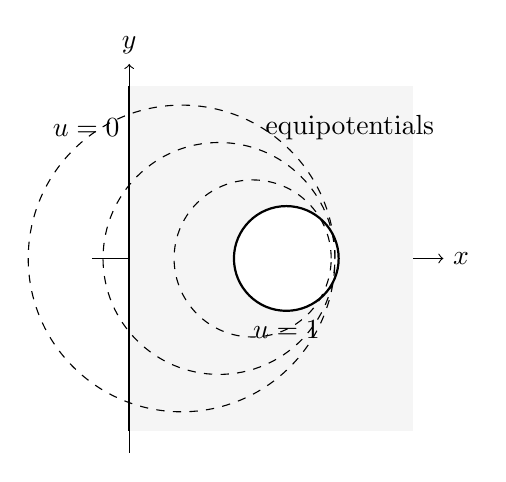
\begin{tikzpicture}[scale=0.95]
  \draw[->] (-0.5,0)--(4.2,0) node[right] {$x$};
  \draw[->] (0,-2.6)--(0,2.6) node[above] {$y$};
  \fill[gray!8] (0,-2.3) rectangle (3.8,2.3);
  \fill[white] (2.1,0) circle (0.7);
  \draw[thick] (0,-2.3)--(0,2.3);
  \draw[thick] (2.1,0) circle (0.7);
  \draw[dashed] (1.65,0) circle (1.05);
  \draw[dashed] (1.2,0) circle (1.55);
  \draw[dashed] (0.7,0) circle (2.05);
  \node[left] at (0,1.75) {$u=0$};
  \node at (2.1,-0.95) {$u=1$};
  \node at (2.95,1.75) {equipotentials};
\end{tikzpicture}
\caption{Pulling concentric circles in the annulus back through the Möbius map gives a coaxal family of equipotential curves in the physical half-plane. They interpolate between the cold $y$-axis and the hot circular obstacle.}
\label{fig:cp-iv-0135-heat-equipotential-curves}
\end{figure}


\begin{solution}
The same conformal normalization solves the heat problem. Put
\[
\alpha=\sqrt{a^2-b^2},
\qquad
\zeta=\frac{z-\alpha}{z+\alpha}.
\]
For \(z=iy\),
\[
|\zeta|=1.
\]
For \(z=a+be^{i\theta}\), the identity
\[
\alpha^2=a^2-b^2
\]
reduces the modulus to the constant
\[
|\zeta|=\rho,
\qquad
\rho=
\sqrt{\frac{a-\alpha}{a+\alpha}}.
\]
Thus
\[
D\longrightarrow\{\rho<|\zeta|<1\}.
\]

The unique radial harmonic function on this annulus with inner value \(1\) and outer value \(0\) is
\[
U(r)=\frac{\log(1/r)}{\log(1/\rho)}.
\]
Consequently
\[
\boxed{
u(z)
=
\frac{
2\log\left|\dfrac{z+\alpha}{z-\alpha}\right|
}{
\log\left(\dfrac{a+\alpha}{a-\alpha}\right)
},
\qquad
\alpha=\sqrt{a^2-b^2}.
}
\]
The maximum principle gives uniqueness among bounded harmonic functions with these boundary data.

The level sets \(u(z)=c\) are the inverse images of the concentric circles
\[
|\zeta|=\rho^c,\qquad 0<c<1.
\]
Hence the isotherms in the original \(z\)-plane form the coaxal family of circles obtained by pulling back those concentric circles through the M\"obius map \(\zeta=(z-\alpha)/(z+\alpha)\).
\end{solution}


\begin{problem}[CP-IV-0138]
\label{prob:cp-iv-0138}
Let $U=\mathbb{C}$ and $f(z)=e^{z}$.

\emph{Existence of $\log f$ on $U$.}
Since $f$ is entire and never zero, $f'/f\equiv 1$ is entire.
Because $U$ is simply connected, $G(z):=z$ is a primitive of $f'/f$.
Define $F(z):=G(z)=z$. Then $e^{F(z)}=e^{z}=f(z)$, so $F$ is a holomorphic branch of $\log f$ on $U$.
Uniqueness holds up to $2\pi i\mathbb{Z}$: if $F_1,F_2$ satisfy $e^{F_j}=f$, then $e^{F_1-F_2}\equiv 1$, hence $F_1-F_2\in 2\pi i\mathbb{Z}$ is a constant.

\medskip

\emph{Failure of a branch of $\log$ on $f(U)$.}
We have $f(U)=\mathbb{C}^\times$.
If there were a holomorphic branch $L$ of the scalar logarithm on $\mathbb{C}^\times$, then $L'(w)=1/w$ and, for every closed loop $\Gamma\subset\mathbb{C}^\times$,
\[
\oint_{\Gamma}\frac{dw}{w}=\oint_{\Gamma}L'(w)\,dw=0.
\]
Taking $\Gamma=\{\,|w|=1\,\}$ yields $\displaystyle\oint_{|w|=1}\frac{dw}{w}=2\pi i\neq 0$, a contradiction.
Therefore, no holomorphic branch of the scalar $\log$ exists on $\mathbb{C}^\times$.

\medskip

\emph{Monodromy/winding viewpoint.}
For any closed loop $\Gamma$ in a domain that avoids $0$,
\[
\oint_{\Gamma}\frac{dw}{w}=2\pi i\cdot \mathrm{Wind}(\Gamma,0).
\]
Thus a global holomorphic branch of $\log$ on a domain $V\subset\mathbb{C}^\times$ exists iff every loop in $V$ has winding number $0$ about $0$ (equivalently, $V$ is simply connected).
Here $V=\mathbb{C}^\times$ has nontrivial loops around $0$, so monodromy obstructs single-valuedness.

\medskip

\emph{Analytic continuation around a circle (explicit jump).}
Start with a local branch of $\log$ near $w=1$ and analytically continue once along the unit circle $w=e^{it}$, $t\in[0,2\pi]$.
The continuation returns to the starting point but accumulates the increment
\[
\int_{0}^{2\pi}\frac{d}{dt}\big(\log(e^{it})\big)\,dt
\;=\;\int_{0}^{2\pi} i\,dt
\;=\;2\pi i,
\]
so the value jumps by $2\pi i$. This nontrivial monodromy forbids a single-valued holomorphic logarithm on $\mathbb{C}^\times$.

\medskip

\emph{Bounded variant (annulus image).}
Let $U=\{z:|z|<2\}$ and $f(z)=e^{z}$. Then $F(z)=z$ gives a branch of $\log f$ on $U$, but
\[
f(U)=\{e^{x+iy}\,:\,|x|<2,\ |y|<2\}
=\{w\in\mathbb{C}^\times: e^{-2}<|w|<e^{2}\},
\]
an annulus encircling $0$. Any circle $\{|w|=r\}$ with $e^{-2}<r<e^{2}$ satisfies $\displaystyle\oint\frac{dw}{w}=2\pi i\neq 0$, so no holomorphic branch of the scalar $\log$ exists on $f(U)$.

\medskip

\emph{Local vs.\ global behavior.}
On any simply connected subdomain $V\subset\mathbb{C}^\times$ that does not wrap around $0$ (e.g.\ a slit plane or a sector of angle $<2\pi$), one \emph{can} choose a holomorphic branch of the scalar $\log$.
The obstruction is purely topological: encircling $0$ forces a $2\pi i$ jump.

\medskip

\emph{Connection with $\arg$ and $f'/f$.}
For $w\neq 0$, $\log w=\log|w|+i\,\arg w$; the impossibility of a global continuous $\arg$ on $\mathbb{C}^\times$ is the same obstruction.
Equivalently, if $L$ existed on $V$, then $(\log\circ f)'=(f'/f)$ would be the derivative of a \emph{global} holomorphic function on $V$.
On simply connected $U$ this always holds for $f'/f$ (hence $\log f$ exists on $U$); on $f(U)$ it fails exactly when some loop winds around $0$.

\medskip

\emph{Takeaway.}
A holomorphic nonvanishing $f$ on a simply connected $U$ always has a holomorphic logarithm $F$ with $e^{F}=f$ (unique up to $2\pi i\mathbb{Z}$).
But a holomorphic scalar logarithm on $f(U)$ may not exist if $f(U)$ winds around $0$ (as with $f=\exp$ giving $\mathbb{C}^\times$ or an annulus).

\par\noindent\textbullet\quad $f$ is entire and never zero, so $f'/f \equiv 1$ is entire.
\par\noindent\textbullet\quad On the simply connected set $U=\mathbb{C}$, a primitive of $f'/f$ is $G(z)=z$.
\par\noindent\textbullet\quad Set $F(z):=G(z)=z$. Then $e^{F(z)}=e^{z}=f(z)$.
Thus $F$ is a (holomorphic) branch of $\log f$ on $U$.

\bigskip

\subsection*{2) Why a holomorphic $\log$ cannot exist on $f(U)=\mathbb{C}^{\times}$}

\par\noindent\textbullet\quad $f(U)=\mathbb{C}\setminus\{0\}$ is not simply connected (its fundamental group is $\mathbb{Z}$);
any loop going once around $0$ has nonzero winding number.
\par\noindent\textbullet\quad If a holomorphic branch of the scalar logarithm $\Log$ existed on $\mathbb{C}^{\times}$, then
$(\Log)'(w)=1/w$ and hence, for every closed loop $\Gamma\subset\mathbb{C}^{\times}$,
\[
\oint_{\Gamma}\frac{dw}{w}
\;=\;
\oint_{\Gamma}(\Log)'(w)\,dw
\;=\;0.
\]
But for the unit circle $\{|w|=1\}$,
\[
\oint_{|w|=1}\frac{dw}{w} \;=\; 2\pi i \;\neq\; 0.
\]
Contradiction. Therefore no holomorphic branch of $\log$ exists on $\mathbb{C}^{\times}$.

\bigskip
\end{problem}

\begin{solution}
For
\[
f(z)=e^z
\]
on \(U=\mathbb C\), the function never vanishes and
\[
\frac{f'}{f}=1.
\]
Since \(U\) is simply connected, this has the global primitive \(z\). Hence
\[
F(z)=z
\]
satisfies
\[
e^{F(z)}=f(z),
\]
so \(F\) is a holomorphic logarithm of \(f\) on \(U\). Any other such logarithm differs from \(F\) by a constant in \(2\pi i\mathbb Z\).

This does not imply that the scalar logarithm has a holomorphic branch on the image
\[
f(U)=\mathbb C^\times.
\]
Indeed, if \(L\) were holomorphic on \(\mathbb C^\times\) and \(e^{L(w)}=w\), then
\[
L'(w)=\frac1w.
\]
Therefore every closed curve \(\Gamma\subset\mathbb C^\times\) would satisfy
\[
\oint_\Gamma\frac{dw}{w}
=
\oint_\Gamma L'(w)\,dw
=
0.
\]
For the unit circle,
\[
\oint_{|w|=1}\frac{dw}{w}=2\pi i,
\]
a contradiction.

Equivalently, analytic continuation of a local logarithm once around \(0\) changes its value by \(2\pi i\). Thus the obstruction is topological: a global branch of \(\log\) on a domain \(V\subset\mathbb C^\times\) can exist only when every closed loop in \(V\) has winding number zero about \(0\).

Hence \(f\) has a global holomorphic logarithm on its simply connected source \(U\), while the scalar logarithm has no global holomorphic branch on the multiply connected image \(\mathbb C^\times\).
\end{solution}


\section{Special Functions}

\par\medskip\noindent\textbf{Related material.}\quad Volume IV, Chapters \texttt{IV/19--IV/21}.

\begin{problem}[CP-IV-0001]
\label{prob:cp-iv-0001}
$f_n(x)=x^n$ on $[0,1]$ converges pointwise to $f=\mathbf{1}_{\{1\}}$ but not uniformly on $(0,1)$.
	\par\noindent\textbullet\quad Pointwise limit of uniformly continuous functions need not be uniformly continuous.
\end{problem}

\begin{solution}
For \(0\le x<1\),
\[
x^n\longrightarrow0,
\]
while
\[
1^n=1.
\]
Thus on \([0,1]\),
\[
f_n(x)=x^n
\]
converges pointwise to
\[
f(x)=
\begin{cases}
0,&0\le x<1,\\
1,&x=1.
\end{cases}
\]
Every \(f_n\) is uniformly continuous on \([0,1]\), because it is continuous on a compact interval. The limit \(f\) is discontinuous at \(1\), hence is not uniformly continuous. This already proves that a pointwise limit of uniformly continuous functions need not be uniformly continuous.

The convergence is not uniform. Indeed,
\[
\sup_{0\le x<1}|x^n-0|=1
\]
for every \(n\), because \(x^n\) can be made arbitrarily close to \(1\) by choosing \(x<1\) sufficiently close to \(1\). Equivalently, on all of \([0,1]\), a uniform limit of the continuous functions \(f_n\) would have to be continuous, whereas the pointwise limit is not.
\end{solution}


\begin{problem}[CP-IV-0002]
\label{prob:cp-iv-0002}
— Disk of radius \(R\)

Parametrize the boundary circle \(C\):
\[
x=R\cos t,\qquad y=R\sin t,\qquad t\in[0,2\pi],
\]
so that
\[
dx=-R\sin t\,dt,\qquad dy=R\cos t\,dt.
\]
Then
\[
\frac12\bigl(x\,dy-y\,dx\bigr)
=
\frac12\Bigl(R\cos t\cdot R\cos t - R\sin t\cdot(-R\sin t)\Bigr)\,dt
=
\frac{R^{2}}{2}\,dt.
\]
Integrate:
\[
\operatorname{Area}
=
\int_{0}^{2\pi} \frac{R^{2}}{2}\,dt
=
\pi R^{2}.
\]
\end{problem}

\begin{solution}
Parametrize the positively oriented circle by
\[
x=R\cos t,\qquad
y=R\sin t,
\qquad
0\le t\le2\pi.
\]
Then
\[
dx=-R\sin t\,dt,
\qquad
dy=R\cos t\,dt.
\]
Therefore
\[
\frac12(x\,dy-y\,dx)
=
\frac12
\left(
R^2\cos^2t+R^2\sin^2t
\right)dt
=
\frac{R^2}{2}\,dt.
\]
Integrating,
\[
\frac12\oint_C(x\,dy-y\,dx)
=
\frac{R^2}{2}\int_0^{2\pi}dt
=
\boxed{\pi R^2}.
\]
This agrees with Green's theorem, since
\[
d\!\left(\frac12(x\,dy-y\,dx)\right)=dx\wedge dy.
\]
\end{solution}


\begin{problem}[CP-IV-0003]
\label{prob:cp-iv-0003}
(ellipse).

For the ellipse
\[
C:\quad \frac{x^{2}}{a^{2}} + \frac{y^{2}}{b^{2}} = 1,
\]
we have
\[
\oint_{C} \tfrac{1}{2}\,\bigl(x\,dy - y\,dx\bigr) \;=\; \pi a b.
\]
(You can parametrize $x=a\cos t$, $y=b\sin t$ and compute directly, or just invoke Green's theorem.)
\end{problem}

\begin{solution}
Use the positively oriented parametrization
\[
x=a\cos t,\qquad
y=b\sin t,
\qquad
0\le t\le2\pi.
\]
Then
\[
dx=-a\sin t\,dt,
\qquad
dy=b\cos t\,dt,
\]
and therefore
\[
\frac12(x\,dy-y\,dx)
=
\frac12
\left(
ab\cos^2t+ab\sin^2t
\right)dt
=
\frac{ab}{2}\,dt.
\]
Hence
\[
\boxed{
\frac12\oint_C(x\,dy-y\,dx)=\pi ab.
}
\]
Thus the differential-form area formula reproduces the usual area of the ellipse.
\end{solution}


\begin{problem}[CP-IV-0006]
\label{prob:cp-iv-0006}
\par\noindent (ii)\quad Let $g$ be an entire function such that $|f(z)|\le |g(z)|$ for all $z\in\mathbb C$.
	Show that there exists $c\in\mathbb C$ such that $f(z)=c\,g(z)$ for all $z\in\mathbb C$.

\bigskip\hrule\bigskip
\end{problem}

\begin{solution}
If \(g\equiv0\), then the inequality
\[
|f(z)|\le|g(z)|=0
\]
forces \(f\equiv0\), and the conclusion holds with \(c=0\).

Assume now that \(g\not\equiv0\). On the set where \(g\neq0\), define
\[
h=\frac{f}{g}.
\]
Then
\[
|h|\le1.
\]
We show that every zero of \(g\) is removable for \(h\). Let \(a\) be a zero of \(g\) of order \(m\):
\[
g(z)=(z-a)^m u(z),
\qquad
u(a)\neq0.
\]
If \(f\not\equiv0\), write
\[
f(z)=(z-a)^n v(z),
\qquad
v(a)\neq0.
\]
The inequality \(|f|\le|g|\) near \(a\) gives
\[
|z-a|^{n-m}\frac{|v(z)|}{|u(z)|}\le1.
\]
This is impossible as \(z\to a\) if \(n<m\). Hence \(n\ge m\), so \(f/g\) extends holomorphically across \(a\).

Thus \(h\) extends to an entire function satisfying \(|h|\le1\). By Liouville's theorem,
\[
h\equiv c
\]
for some \(c\in\mathbb C\), with \(|c|\le1\). Consequently
\[
\boxed{f=cg}.
\]
\end{solution}


\begin{problem}[CP-IV-0010]
\label{prob:cp-iv-0010}
Evaluate the following integrals.

\medskip
\emph{(a)} $\displaystyle \int_{0}^{\pi}\frac{d\theta}{4+\sin^{2}\theta}$.

Using $\displaystyle \int_{0}^{\pi}\frac{d\theta}{a+b\sin^{2}\theta}
=\frac{\pi}{\sqrt{a(a+b)}}$ for $a>0$, with $a=4$, $b=1$,
\[
\int_{0}^{\pi}\frac{d\theta}{4+\sin^{2}\theta}
=\frac{\pi}{\sqrt{4\cdot 5}}=\boxed{\frac{\pi}{2\sqrt5}}.
\]

\medskip
\emph{(b)} $\displaystyle \int_{0}^{\infty}\sin(x^{2})\,dx$.

By the Fresnel/Gaussian argument,
\[
\int_{0}^{\infty}\sin(x^{2})\,dx
=\int_{0}^{\infty}\cos(x^{2})\,dx
=\boxed{\frac{\sqrt{2\pi}}{4}=\frac{\sqrt{\pi}}{2\sqrt2}}.
\]

\medskip
\emph{(c)} $\displaystyle \int_{0}^{\infty}\frac{x^{2}}{(x^{2}+4)^{2}(x^{2}+9)}\,dx$.

Let $f(z)=\dfrac{z^{2}}{(z^{2}+4)^{2}(z^{2}+9)}$. The integrand is even; hence
\[
\int_{0}^{\infty}f(x)\,dx=\frac12\int_{-\infty}^{\infty}f(x)\,dx.
\]
Poles in the upper half-plane: $2i$ (double), $3i$ (simple).
\[
\operatorname{Res}(f;2i)=-\frac{13i}{200},\qquad \operatorname{Res}(f;3i)=\frac{3i}{50},\qquad
\operatorname{Res}(f;2i)+\operatorname{Res}(f;3i)=-\frac{i}{200}.
\]
Thus
\[
\int_{-\infty}^{\infty} f(x)\,dx
=2\pi i\!\left(-\frac{i}{200}\right)=\frac{\pi}{100},
\qquad
\int_{0}^{\infty} f(x)\,dx=\boxed{\frac{\pi}{200}}.
\]

\medskip
\emph{(d)} $\displaystyle \int_{0}^{\infty}\frac{\ln(x^{2}+1)}{x^{2}+1}\,dx$.

With $x=\tan t$ ($t\in[0,\pi/2)$), $x^{2}+1=\sec^{2}t$, $dx=\sec^{2}t\,dt$,
\[
\int_{0}^{\infty}\frac{\ln(x^{2}+1)}{x^{2}+1}\,dx
=\int_{0}^{\pi/2}\ln(\sec^{2}t)\,dt
=2\int_{0}^{\pi/2}\ln(\sec t)\,dt
=-2\int_{0}^{\pi/2}\ln(\cos t)\,dt
=\boxed{\pi\ln 2}.
\]

\end{problem}

\begin{solution}
For
\[
I_1=\int_0^\pi\frac{d\theta}{4+\sin^2\theta},
\]
use
\[
\int_0^\pi\frac{d\theta}{a+b\sin^2\theta}
=
\frac{\pi}{\sqrt{a(a+b)}}
\qquad(a>0).
\]
With \(a=4\), \(b=1\),
\[
\boxed{I_1=\frac{\pi}{2\sqrt5}}.
\]

For the Fresnel integral,
\[
\int_0^\infty e^{ix^2}\,dx
=
e^{i\pi/4}\int_0^\infty e^{-t^2}\,dt
=
e^{i\pi/4}\frac{\sqrt\pi}{2},
\]
obtained by rotating the Gaussian contour through \(\pi/4\). Taking imaginary parts,
\[
\boxed{
\int_0^\infty\sin(x^2)\,dx
=
\frac{\sqrt\pi}{2\sqrt2}.
}
\]

For
\[
I_3
=
\int_0^\infty
\frac{x^2\,dx}{(x^2+4)^2(x^2+9)},
\]
the integrand is even. In the upper half-plane the poles are \(2i\) (double) and \(3i\) (simple), with
\[
\operatorname{Res}(f;2i)=-\frac{13i}{200},
\qquad
\operatorname{Res}(f;3i)=\frac{3i}{50}.
\]
Their sum is
\[
-\frac{i}{200}.
\]
Hence
\[
\int_{-\infty}^{\infty}f(x)\,dx
=
2\pi i\left(-\frac{i}{200}\right)
=
\frac{\pi}{100},
\]
so
\[
\boxed{I_3=\frac{\pi}{200}}.
\]

Finally, with \(x=\tan t\),
\[
dx=\sec^2t\,dt,
\qquad
1+x^2=\sec^2t,
\]
and
\[
\int_0^\infty\frac{\log(1+x^2)}{1+x^2}\,dx
=
2\int_0^{\pi/2}\log(\sec t)\,dt.
\]
Using
\[
\int_0^{\pi/2}\log(\cos t)\,dt
=
-\frac{\pi}{2}\log2,
\]
we obtain
\[
\boxed{
\int_0^\infty\frac{\log(1+x^2)}{1+x^2}\,dx
=
\pi\log2.
}
\]
\end{solution}


\begin{problem}[CP-IV-0011]
\label{prob:cp-iv-0011}
\par\noindent\textbullet\quad If $f_n \Rightarrow f$ uniformly on $\mathbb{R}$, prove that $f$ is uniformly continuous.
\end{problem}

\begin{solution}
Let \(\varepsilon>0\). Since \(f_n\to f\) uniformly on \(\mathbb R\), choose \(N\) such that
\[
|f_N(x)-f(x)|<\frac{\varepsilon}{3}
\qquad\text{for every }x\in\mathbb R.
\]
The single function \(f_N\) is uniformly continuous, so there exists \(\delta>0\) such that
\[
|x-y|<\delta
\quad\Longrightarrow\quad
|f_N(x)-f_N(y)|<\frac{\varepsilon}{3}.
\]
Then
\[
\begin{aligned}
|f(x)-f(y)|
&\le
|f(x)-f_N(x)|
+
|f_N(x)-f_N(y)|
+
|f_N(y)-f(y)|\\
&<
\frac{\varepsilon}{3}
+
\frac{\varepsilon}{3}
+
\frac{\varepsilon}{3}
=
\varepsilon.
\end{aligned}
\]
The same \(\delta\) works for every \(x,y\in\mathbb R\). Therefore \(f\) is uniformly continuous.
\end{solution}


\begin{problem}[CP-IV-0013]
\label{prob:cp-iv-0013}
\par\noindent\textbullet\quad (\textbf{Jacobian, determinant, and orientation})
	Show the Jacobian determinant of $T$ equals
	\[
	\det DT=|A|^2-|B|^2.
	\]
	Conclude that $T$ is orientation-preserving iff $|A|>|B|$, reversing iff $|A|<|B|$, and singular iff $|A|=|B|$.

	\emph{Solution.} Using Ex.\ 3’s matrix and a short computation:
	$\det=\!(\alpha+\gamma)(\alpha-\gamma)-(-\beta+\delta)(\beta+\delta)
	=(\alpha^2+\beta^2)-(\gamma^2+\delta^2)=|A|^2-|B|^2$.
\end{problem}

\begin{solution}
Write
\[
A=\alpha+i\beta,
\qquad
B=\gamma+i\delta,
\qquad
z=x+iy.
\]
Then
\[
Az+B\overline z
=
\bigl((\alpha+\gamma)x+(-\beta+\delta)y\bigr)
+
i\bigl((\beta+\delta)x+(\alpha-\gamma)y\bigr).
\]
Hence the real matrix of \(T\) is
\[
DT=
\begin{pmatrix}
\alpha+\gamma&-\beta+\delta\\
\beta+\delta&\alpha-\gamma
\end{pmatrix}.
\]
Its determinant is
\[
\begin{aligned}
\det DT
&=
(\alpha+\gamma)(\alpha-\gamma)
-
(-\beta+\delta)(\beta+\delta)\\
&=
\alpha^2+\beta^2-\gamma^2-\delta^2\\
&=
|A|^2-|B|^2.
\end{aligned}
\]
Therefore
\[
\boxed{\det DT=|A|^2-|B|^2}.
\]
Thus \(T\) preserves orientation when \(|A|>|B|\), reverses orientation when \(|A|<|B|\), and is singular precisely when
\[
|A|=|B|.
\]
\end{solution}


\begin{problem}[CP-IV-0018]
\label{prob:cp-iv-0018}
\par\noindent\textbullet\quad If $X=\mathbb{R}$, does $(f_n)$ still necessarily have a pointwise convergent subsequence?
\end{problem}

\begin{solution}
\par\medskip\noindent\textbf{(a) $X=\mathbb{N}$.}\quad 
For each fixed $m\in\mathbb{N}$ the real sequence $(f_n(m))_{n\ge1}$ is bounded, hence has a convergent subsequence.
Construct subsequences by diagonalization:

	\par\noindent\textbullet\quad pick $(n^{(1)}_k)$ so that $f_{n^{(1)}_k}(1)$ converges;
	\par\noindent\textbullet\quad from that, pick $(n^{(2)}_k)$ so that $f_{n^{(2)}_k}(2)$ also converges;
	\par\noindent\textbullet\quad continue inductively.

Define $m_k:=n^{(k)}_k$. Then for each fixed $j$, the tail $(f_{m_k}(j))_{k\ge j}$ coincides with a tail of $(f_{n^{(j)}_k}(j))$, hence converges. Therefore $(f_{m_k})$ converges \emph{pointwise on $\mathbb{N}$}.

\par\medskip\noindent\textbf{(b) $X=\mathbb{R}$.}\quad 
Not necessarily. Consider the Rademacher functions on $[0,1]$,
\[
r_n(x)=\operatorname{sign}(\sin(2^n\pi x))\in\{-1,1\},
\]
extended to $\mathbb{R}$ periodically. They satisfy $|r_n(x)|\le 1$ for all $x,n$, so the family is pointwise bounded.

We claim no subsequence of $(r_n)$ converges pointwise on $[0,1]$. Let $(r_{n_k})$ be any subsequence. Choose $x\in[0,1]$ whose binary digits at positions $n_k$ alternate $0,1,0,1,\dots$ (fill other digits arbitrarily and avoid a terminating expansion). For this $x$,
\[
r_{n_k}(x)=(-1)^{\text{binary digit of $x$ at position $n_k$}}
\]
alternates between $+1$ and $-1$, hence does not converge. Thus no subsequence converges pointwise on all of $[0,1]$ (and hence not on $\mathbb{R}$).

\par\medskip\noindent\textbf{Conclusion.}\quad 
(a) Yes: a pointwise convergent subsequence exists by diagonalization on the countable domain.
(b) No: on $\mathbb{R}$, pointwise boundedness alone does not ensure a pointwise convergent subsequence.
\end{solution}

\begin{problem}[CP-IV-0021]
\label{prob:cp-iv-0021}
\par\noindent (i)\quad Prove that $f$ is a polynomial of degree at most $k$ if and only if there exist real constants $M,R>0$ and an integer $k$ such that
	\[
	|f(z)|\le M\,|z|^{k}\qquad\text{for }|z|>R.
	\]
\end{problem}

\begin{solution}
Assume throughout that \(f\) is entire.

If \(f\) is a polynomial of degree at most \(k\), then
\[
f(z)=a_0+a_1z+\cdots+a_kz^k.
\]
For \(|z|\ge1\),
\[
|f(z)|
\le
\left(\sum_{j=0}^k|a_j|\right)|z|^k,
\]
so the required growth estimate holds.

Conversely, suppose that for some \(M,R>0\),
\[
|f(z)|\le M|z|^k
\qquad(|z|>R).
\]
Fix an integer \(n>k\). For every \(r>R\), Cauchy's estimate on \(|z|=r\) gives
\[
|f^{(n)}(0)|
\le
\frac{n!}{r^n}\max_{|z|=r}|f(z)|
\le
n!M r^{k-n}.
\]
Since \(k-n<0\), letting \(r\to\infty\) yields
\[
f^{(n)}(0)=0.
\]
This holds for every \(n>k\). Hence the Taylor expansion of the entire function \(f\) terminates after degree \(k\), and therefore \(f\) is a polynomial of degree at most \(k\).
\end{solution}


\begin{problem}[CP-IV-0022]
\label{prob:cp-iv-0022}
(unit circle).

For $\Gamma=\{|\zeta|=1\}$ and $f(\zeta)=\zeta^{m}$ ($m\ge0$):
	\[
	F(z)=\begin{cases} z^{m}, & |z|<1,\\ 0, & |z|>1,\end{cases}
	\quad\Rightarrow\quad
	F^{+}(e^{it})-F^{-}(e^{it})=e^{im t}=f(e^{it}),
	\]
	and
	\(
	\operatorname{P.V.}\,\frac{1}{2\pi i}\int_{|\zeta|=1}\frac{\zeta^{m}}{\zeta-e^{it}}\,d\zeta
	=\tfrac12 e^{imt}.
	\)

	The Plemelj formulas remain valid for \emph{Lipschitz} curves (e.g.\ piecewise $C^{1}$ with finite length) when boundary limits are taken \emph{nontangentially}.
	This is classical in singular–integral theory (Calder\'on–Zygmund): the Cauchy singular integral operator is bounded on $L^{p}(\Gamma)$ for $1<p<\infty$, and the nontangential boundary limits exist almost everywhere.

	\medskip

		\par\noindent\textbullet\quad For classical \emph{pointwise} limits at every boundary point, it suffices to assume $f\in C^{0,\alpha}(\Gamma)$ (H\"older) for some $\alpha\in(0,1]$.
		\par\noindent\textbullet\quad For \emph{almost-everywhere} (a.e.) limits and $L^{p}$ jump relations, it is enough to assume $f\in L^{p}(\Gamma)$ with $1<p<\infty$.
		\par\noindent\textbullet\quad The original hypothesis $f\in C^{1}(\Gamma)$ is more than enough; it guarantees the principal value is well defined and that the interior/exterior limits exist \emph{at every} $\zeta_{0}\in\Gamma$ (no exceptional set).
\end{problem}

% Designed Companion Part IV figure
% Intended for \input{...} beside the matching canonical problem.
\begin{figure}[ht]
\centering
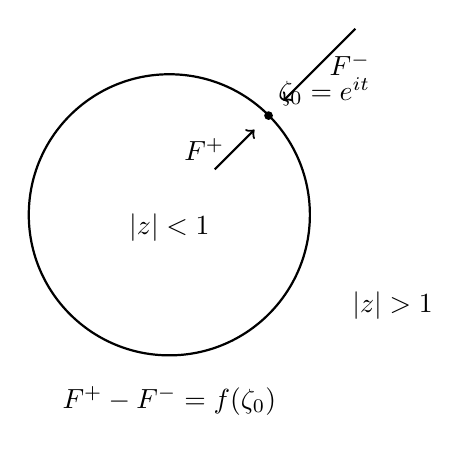
\begin{tikzpicture}[scale=1.05]
  \draw[thick] (0,0) circle (1.7);
  \fill (1.2,1.2) circle (1.5pt) node[above right] {$\zeta_0=e^{it}$};
  \draw[->,thick] (0.55,0.55)--(1.03,1.03) node[midway,left] {$F^+$};
  \draw[->,thick] (2.25,2.25)--(1.38,1.38) node[midway,right] {$F^-$};
  \node at (0,-0.15) {$|z|<1$};
  \node at (2.7,-1.1) {$|z|>1$};
  \node at (0,-2.25) {$F^+-F^-=f(\zeta_0)$};
\end{tikzpicture}
\caption{Nontangential limits of the Cauchy transform approach the same boundary point $\zeta_0$ from the interior and exterior. Their jump is $F^+(\zeta_0)-F^-(\zeta_0)=f(\zeta_0)$.}
\label{fig:cp-iv-0022-plemelj-unit-circle}
\end{figure}


\begin{solution}
Let
\[
F(z)
=
\frac{1}{2\pi i}
\int_{|\zeta|=1}
\frac{\zeta^m}{\zeta-z}\,d\zeta,
\qquad m\ge0.
\]
If \(|z|<1\), Cauchy's formula gives
\[
F(z)=z^m.
\]
If \(|z|>1\), the integrand has no pole inside the unit circle, so
\[
F(z)=0.
\]
Therefore, for \(\zeta_0=e^{it}\),
\[
F^+(\zeta_0)=\zeta_0^m,
\qquad
F^-(\zeta_0)=0.
\]
The Plemelj formulas become
\[
F^\pm(\zeta_0)
=
\operatorname{P.V.}\,
\frac{1}{2\pi i}
\int_{|\zeta|=1}
\frac{\zeta^m}{\zeta-\zeta_0}\,d\zeta
\pm\frac12\zeta_0^m.
\]
Subtracting gives the jump relation
\[
F^+-F^-=\zeta_0^m,
\]
and averaging gives
\[
\boxed{
\operatorname{P.V.}\,
\frac{1}{2\pi i}
\int_{|\zeta|=1}
\frac{\zeta^m}{\zeta-e^{it}}\,d\zeta
=
\frac12e^{imt}.
}
\]

For pointwise boundary limits at every point, a Hölder condition
\[
f\in C^{0,\alpha}(\Gamma),
\qquad 0<\alpha\le1,
\]
is sufficient. For almost-everywhere nontangential limits and \(L^p\) jump relations on a Lipschitz curve, the classical singular-integral theory allows
\[
f\in L^p(\Gamma),
\qquad 1<p<\infty.
\]
Thus the original \(C^1\) hypothesis is stronger than necessary.
\end{solution}


\begin{problem}[CP-IV-0026]
\label{prob:cp-iv-0026}
\par\noindent\textbullet\quad $\{(x,y): y\ne 0\}$.
\end{problem}

\begin{solution}
Let
\[
U=\{(x,y)\in\mathbb R^2:y\neq0\}.
\]
This is
\[
U=\{y>0\}\cup\{y<0\},
\]
a union of two open half-planes, so \(U\) is open.

It is not closed. For example,
\[
(0,1/n)\in U
\]
for every \(n\), but
\[
(0,1/n)\longrightarrow(0,0)\notin U.
\]
Equivalently, the complement
\[
\{(x,0):x\in\mathbb R\}
\]
is closed but not open. Therefore
\[
\boxed{U\text{ is open and not closed}.}
\]
\end{solution}


\begin{problem}[CP-IV-0028]
\label{prob:cp-iv-0028}
Let $(f_n)$ and $(g_n)$ be sequences of real-valued functions on a set $X$ with
$f_n \xRightarrow{\text{\rm unif}} f$ and $g_n \xRightarrow{\text{\rm unif}} g$.

\par\noindent\textbullet\quad Show that $f_n+g_n \xRightarrow{\text{\rm unif}} f+g$.
\par\noindent\textbullet\quad Show that $f_n g_n \to fg$ pointwise, but that $f_n g_n$ need not converge uniformly to $fg$ in general. If $f$ and $g$ are bounded, does the latter conclusion change? What if $f$ is bounded but $g$ is not?

Uniform convergence means $\|f_n-f\|_\infty=\sup_{x\in X}|f_n(x)-f(x)|\to 0$; it implies pointwise convergence. For products we use
\[
|f_n g_n - fg| \le |f_n|\,|g_n-g| + |g|\,|f_n-f|.
\]
If $f_n\Rightarrow f$, then $f_n$ are eventually uniformly bounded.
\end{problem}

\begin{solution}
Let $\varepsilon>0$. Choose $N_1$ with $\sup_X|f_n-f|<\varepsilon/2$ for $n\ge N_1$ and $N_2$ with $\sup_X|g_n-g|<\varepsilon/2$ for $n\ge N_2$. For $n\ge N=\max\{N_1,N_2\}$,
\[
\sup_{x\in X}|(f_n+g_n)-(f+g)| \le \sup_X|f_n-f|+\sup_X|g_n-g| < \varepsilon,
\]
hence $f_n+g_n \Rightarrow f+g$.
\end{solution}

\begin{problem}[CP-IV-0030]
\label{prob:cp-iv-0030}
\par\noindent\textbullet\quad $\{(x,0): 0\le x\le 1\}$.
\end{problem}

\begin{solution}
Let
\[
S=\{(x,0):0\le x\le1\}.
\]
It is closed because
\[
S
=
\{(x,y):y=0\}
\cap
\{(x,y):0\le x\le1\},
\]
and both sets on the right are closed in \(\mathbb R^2\). Equivalently, \(S\) is compact, hence closed.

It is not open: every Euclidean ball centered at a point of \(S\) contains points with \(y\neq0\), so no point of \(S\) is an interior point in \(\mathbb R^2\).

Hence
\[
\boxed{S\text{ is closed and not open}.}
\]
\end{solution}


\begin{problem}[CP-IV-0032]
\label{prob:cp-iv-0032}
$f(x)=x^2$ on $\mathbb{R}$ is not uniformly continuous.
	\par\noindent\textbullet\quad Pointwise convergence $\nRightarrow$ uniform convergence.
\end{problem}

\begin{solution}
The function
\[
f(x)=x^2
\]
is not uniformly continuous on \(\mathbb R\). Take
\[
x_n=n,
\qquad
y_n=n+\frac1n.
\]
Then
\[
|x_n-y_n|=\frac1n\longrightarrow0,
\]
but
\[
|f(y_n)-f(x_n)|
=
\left(n+\frac1n\right)^2-n^2
=
2+\frac1{n^2}
\longrightarrow2.
\]
Thus arbitrarily close inputs can have outputs separated by nearly \(2\), contradicting uniform continuity.

Pointwise convergence also does not imply uniform convergence. For example,
\[
f_n(x)=x^n
\]
on \([0,1]\) converges pointwise to
\[
f(x)=
\begin{cases}
0,&0\le x<1,\\
1,&x=1,
\end{cases}
\]
but the convergence is not uniform. Indeed the pointwise limit is discontinuous, whereas a uniform limit of continuous functions would be continuous. Equivalently,
\[
\sup_{0\le x<1}x^n=1
\]
for every \(n\).
\end{solution}


\begin{problem}[CP-IV-0033]
\label{prob:cp-iv-0033}
\par\noindent\textbullet\quad Show that the map $f \mapsto \displaystyle\Big(x\mapsto \int_a^x f(y)\,dy\Big)$ is a continuous map from $C^k([a,b])$ to $C^{k+1}([a,b])$.
\end{problem}

\begin{solution}
Define
\[
(Tf)(x)=\int_a^x f(y)\,dy.
\]
The map \(T\) is linear. By the fundamental theorem of calculus,
\[
(Tf)'=f,
\]
and therefore, for \(j=1,\ldots,k+1\),
\[
(Tf)^{(j)}=f^{(j-1)}.
\]
Also
\[
\|Tf\|_\infty
\le
(b-a)\|f\|_\infty.
\]

Using the standard norm
\[
\|f\|_{C^k}
=
\sum_{j=0}^k\|f^{(j)}\|_\infty,
\]
we obtain
\[
\begin{aligned}
\|Tf\|_{C^{k+1}}
&=
\|Tf\|_\infty
+
\sum_{j=1}^{k+1}\|(Tf)^{(j)}\|_\infty\\
&\le
(b-a)\|f\|_\infty
+
\sum_{j=0}^k\|f^{(j)}\|_\infty\\
&\le
\bigl(1+b-a\bigr)\|f\|_{C^k}.
\end{aligned}
\]
Hence \(T:C^k([a,b])\to C^{k+1}([a,b])\) is a bounded linear operator, and therefore it is continuous.
\end{solution}


\begin{problem}[CP-IV-0038]
\label{prob:cp-iv-0038}
\par\noindent\textbullet\quad Not necessarily. For example,
	\[
	f(z)=z^{2}+\sin(\pi z)
	\]
	is entire and satisfies $f(n)=n^{2}$ for all $n\in\mathbb Z$, yet $f\not\equiv z^{2}$.

	\medskip
\end{problem}

\begin{solution}
No. The values of an entire function on \(\mathbb Z\) do not determine it uniquely, because \(\mathbb Z\) has no accumulation point in \(\mathbb C\).

A concrete counterexample is
\[
f(z)=z^2+\sin(\pi z).
\]
This function is entire, and for every \(n\in\mathbb Z\),
\[
f(n)=n^2+\sin(\pi n)=n^2.
\]
However,
\[
f\not\equiv z^2,
\]
because \(\sin(\pi z)\) is not identically zero.

This does not contradict the identity theorem: that theorem requires the set on which two holomorphic functions agree to have an accumulation point inside the domain. The integers have no finite accumulation point in \(\mathbb C\).
\end{solution}


\begin{problem}[CP-IV-0040]
\label{prob:cp-iv-0040}
\par\noindent\textbullet\quad $A=\{f\in C([0,1]) : f(1/2)=0\}$;
\end{problem}

\begin{solution}
Assume \(C([0,1])\) is equipped with the standard sup norm
\[
\|f\|_\infty=\sup_{x\in[0,1]}|f(x)|.
\]
Consider
\[
A=\{f\in C([0,1]):f(1/2)=0\}.
\]
The evaluation functional
\[
E_{1/2}:C([0,1])\to\mathbb R,
\qquad
E_{1/2}(f)=f(1/2),
\]
is continuous because
\[
|E_{1/2}(f)-E_{1/2}(g)|
=
|f(1/2)-g(1/2)|
\le
\|f-g\|_\infty.
\]
Hence
\[
A=E_{1/2}^{-1}(\{0\})
\]
is closed.

It is not open. If \(f\in A\) and \(\varepsilon>0\), define
\[
g(x)=f(x)+\frac{\varepsilon}{2}.
\]
Then
\[
\|g-f\|_\infty=\frac{\varepsilon}{2}<\varepsilon,
\]
but
\[
g(1/2)=\frac{\varepsilon}{2}\neq0.
\]
Thus every sup-norm ball about a point of \(A\) meets the complement of \(A\).

Therefore \(A\) is a closed, non-open linear subspace of \(C([0,1])\).
\end{solution}


\begin{problem}[CP-IV-0041]
\label{prob:cp-iv-0041}
\par\noindent\textbullet\quad If $X=\mathbb{N}$, show that $(f_n)$ has a pointwise convergent subsequence.
\end{problem}

\begin{solution}
Under the ambient hypothesis that the sequence is pointwise bounded, the conclusion follows by a diagonal argument.

Write
\[
X=\mathbb N.
\]
Since \((f_n(1))_{n\ge1}\) is a bounded sequence of scalars, it has a convergent subsequence; call its indices
\[
n^{(1)}_1<n^{(1)}_2<\cdots.
\]
From that subsequence, choose a further subsequence
\[
n^{(2)}_1<n^{(2)}_2<\cdots
\]
such that \(f_{n^{(2)}_k}(2)\) converges. Continue inductively: at stage \(j\), choose a subsequence along which the value at \(j\) converges.

Now take the diagonal sequence
\[
m_k:=n^{(k)}_k.
\]
Fix \(j\). For \(k\ge j\), the index \(m_k\) belongs to the \(j\)-th subsequence, so
\[
f_{m_k}(j)
\]
is a tail of a convergent scalar sequence. Hence it converges.

Therefore
\[
f_{m_k}(j)
\]
converges for every \(j\in\mathbb N\), i.e. \((f_{m_k})\) converges pointwise on \(\mathbb N\).

The pointwise-boundedness assumption is essential: without it, even at a single point the scalar sequence need not have a convergent subsequence.
\end{solution}


\begin{problem}[CP-IV-0042]
\label{prob:cp-iv-0042}
$f_n(x)=\sin(x)/n\to 0$ uniformly on $\mathbb{R}$.

	\par\noindent\textbullet\quad \textbf{Inclusion and restriction.}
	If $Y\subset X$ (subspace topology), the inclusion $i:Y\hookrightarrow X$ is continuous.
	If $f:X\to Z$ is continuous, then $f|_Y$ is continuous.

	\par\noindent\textbullet\quad \textbf{Continuous need not be closed.}
	$f:\mathbb{R}\to\mathbb{R}$, $f(x)=e^x$ is continuous but sends the closed set $\mathbb{R}$ to $(0,\infty)$, which is not closed.
\end{problem}

\begin{solution}
For
\[
f_n(x)=\frac{\sin x}{n},
\]
we have
\[
|f_n(x)|
\le
\frac1n
\qquad (x\in\mathbb R).
\]
Therefore
\[
\|f_n\|_\infty
=
\sup_{x\in\mathbb R}\frac{|\sin x|}{n}
=
\frac1n
\longrightarrow0,
\]
so \(f_n\to0\) uniformly on \(\mathbb R\).

If \(Y\subset X\) has the subspace topology, the inclusion
\[
i:Y\hookrightarrow X
\]
is continuous because for every open \(U\subset X\),
\[
i^{-1}(U)=U\cap Y,
\]
which is open in \(Y\).

If \(f:X\to Z\) is continuous, then the restriction
\[
f|_Y:Y\to Z
\]
is continuous, since for every open \(V\subset Z\),
\[
(f|_Y)^{-1}(V)
=
Y\cap f^{-1}(V),
\]
which is open in the subspace \(Y\).

Finally, continuity does not imply that a map is closed. The map
\[
f:\mathbb R\to\mathbb R,
\qquad
f(x)=e^x,
\]
is continuous, but the closed set \(\mathbb R\) is mapped to
\[
(0,\infty),
\]
which is not closed in \(\mathbb R\).
\end{solution}


\begin{problem}[CP-IV-0045]
\label{prob:cp-iv-0045}
Schwarz--Christoffel map from the half-plane to a rectangle

Write down, as an integral, the Schwarz--Christoffel map from the upper half-plane \(\mathbb H\) to a rectangle,
	with vertices being the images of the points \(z=\pm1\) and \(z=\pm a\) (with \(a>1\) real).
	Explain why \(a\) cannot be chosen arbitrarily, but is determined by the rectangle’s aspect ratio.

	For prevertices \(x_k\in\mathbb R\) mapping to interior angles \(\alpha_k\pi\) in the polygon,
	\[
	f'(z)=C\prod_k (z-x_k)^{\alpha_k-1}\qquad\text{(up to an affine change of variables).}
	\]
	A rectangle has \(\alpha_k=\tfrac12\) at each vertex, so every factor’s exponent is \(-\tfrac12\).
\end{problem}

\begin{solution}
Place prevertices at \(-a,-1,1,a\) (in order) with \(a>1\).
	Then
	\[
	f'(z)=C\,(z{+}a)^{-1/2}(z{+}1)^{-1/2}(z{-}1)^{-1/2}(z{-}a)^{-1/2}
	=\frac{C}{\sqrt{(z^{2}-1)(z^{2}-a^{2})}}.
	\]
	Integrating,
	\[
	\boxed{\qquad f(z)=A+C\int^{\,z}\frac{dt}{\sqrt{(t^{2}-1)(t^{2}-a^{2})}}\qquad}
	\]
	maps \(\mathbb H\) conformally to a rectangle (up to translation and scaling).
\end{solution}

\begin{problem}[CP-IV-0046]
\label{prob:cp-iv-0046}
— Triangle with vertices \((0,0)\to(2,1)\to(1,3)\to(0,0)\)

Integrate \(\tfrac12(x\,dy-y\,dx)\) edge by edge (CCW orientation).

Parametrize \(x=2t\), \(y=t\), \(t\in[0,1]\). Then \(dx=2\,dt\), \(dy=dt\), and
\[
\frac12(x\,dy-y\,dx)
=
\frac12\,(2t\cdot dt - t\cdot 2\,dt)
=
0
\quad\Rightarrow\quad \text{contribution }=0.
\]

Parametrize \(x=2-s\), \(y=1+2s\), \(s\in[0,1]\). Then \(dx=-ds\), \(dy=2\,ds\), and
\[
\frac12(x\,dy-y\,dx)
=
\frac12\Bigl((2-s)\cdot 2 - (1+2s)\cdot(-1)\Bigr)\,ds
=
\frac{5}{2}\,ds.
\]
Contribution:
\[
\int_{0}^{1}\frac{5}{2}\,ds=\frac{5}{2}=2.5.
\]

Parametrize \(x=1-t\), \(y=3-3t\), \(t\in[0,1]\). Then \(dx=-dt\), \(dy=-3\,dt\), and
\[
\frac12(x\,dy-y\,dx)
=
\frac12\Bigl((1-t)(-3) - (3-3t)(-1)\Bigr)\,dt
=
0
\quad\Rightarrow\quad \text{contribution }=0.
\]

\[
\operatorname{Area}=0+2.5+0=\boxed{2.5}.
\]
(Checks the shoelace formula:
\(\displaystyle \tfrac12\bigl|0\cdot1+2\cdot3+1\cdot0-(2\cdot0+1\cdot1+0\cdot3)\bigr|
=\tfrac12|6-1|=2.5\).)
\end{problem}

\begin{solution}
Let the positively oriented triangle have vertices
\[
(0,0)\longrightarrow(2,1)\longrightarrow(1,3)\longrightarrow(0,0).
\]
We evaluate
\[
\frac12\oint_C(x\,dy-y\,dx)
\]
edge by edge.

On the first edge, use
\[
x=2t,\qquad y=t,\qquad 0\le t\le1.
\]
Then
\[
dx=2\,dt,\qquad dy=dt,
\]
and
\[
\frac12(x\,dy-y\,dx)
=
\frac12(2t-2t)\,dt
=
0.
\]

On the second edge, use
\[
x=2-s,\qquad y=1+2s,\qquad 0\le s\le1.
\]
Then
\[
dx=-ds,\qquad dy=2\,ds,
\]
so
\[
\frac12(x\,dy-y\,dx)
=
\frac12\bigl(2(2-s)+(1+2s)\bigr)\,ds
=
\frac52\,ds.
\]
Thus this edge contributes
\[
\frac52.
\]

On the third edge, use
\[
x=1-t,\qquad y=3-3t,\qquad 0\le t\le1.
\]
Then
\[
dx=-dt,\qquad dy=-3\,dt,
\]
and again
\[
\frac12(x\,dy-y\,dx)=0.
\]

Hence
\[
\boxed{
\operatorname{Area}
=
\frac12\oint_C(x\,dy-y\,dx)
=
\frac52.
}
\]
This agrees with the shoelace formula.
\end{solution}


\begin{problem}[CP-IV-0049]
\label{prob:cp-iv-0049}
Evaluate
\[
I=\int_{0}^{\infty}\frac{x^{1/2}\,\log x}{(1+x)^2}\,dx .
\]

\bigskip

For \(0<a<2\) the Beta–Gamma identity gives
\[
F(a):=\int_{0}^{\infty}\frac{x^{a-1}}{(1+x)^2}\,dx
=B(a,2-a)=\Gamma(a)\Gamma(2-a).
\]
Differentiation under the parameter is legitimate here, and since
\(\dfrac{d}{da}x^{a-1}=x^{a-1}\log x\), we obtain integrals with a \(\log x\) factor
by differentiating \(F\).
We also use the digamma function \(\psi=\Gamma'/\Gamma\) and the values
\(\psi(\tfrac12)=-\gamma-2\log2\), \(\psi(\tfrac32)=\psi(\tfrac12)+2\).

\bigskip
\end{problem}

\begin{solution}
Differentiate \(F\):
\[
F'(a)=\int_{0}^{\infty}\frac{x^{a-1}\log x}{(1+x)^2}\,dx
=\frac{d}{da}\big(\Gamma(a)\Gamma(2-a)\big)
=\Gamma(a)\Gamma(2-a)\big(\psi(a)-\psi(2-a)\big).
\]
We need \(I=F'(3/2)\).  Compute
\[
F\!\left(\tfrac32\right)
=\Gamma\!\left(\tfrac32\right)\Gamma\!\left(\tfrac12\right)
=\frac{\sqrt\pi}{2}\cdot\sqrt\pi=\frac{\pi}{2},
\qquad
\psi\!\left(\tfrac32\right)-\psi\!\left(\tfrac12\right)=2.
\]
Therefore
\[
I=F'\!\left(\tfrac32\right)
=\frac{\pi}{2}\cdot 2
=\boxed{\pi}.
\]

\bigskip
\end{solution}

\begin{problem}[CP-IV-0050]
\label{prob:cp-iv-0050}
\par\noindent\textbullet\quad $f_n(x)=x e^{-nx}$ on $X=[0,\infty)$.
\end{problem}

\begin{solution}
For
\[
f_n(x)=xe^{-nx},
\qquad x\ge0,
\]
we first have pointwise convergence:
\[
f_n(0)=0,
\]
and for every fixed \(x>0\),
\[
xe^{-nx}\longrightarrow0.
\]
Thus \(f_n(x)\to0\) pointwise on \([0,\infty)\).

To test uniform convergence, maximize
\[
g_n(x)=xe^{-nx}.
\]
Its derivative is
\[
g_n'(x)=e^{-nx}(1-nx),
\]
so the unique interior maximum occurs at
\[
x=\frac1n.
\]
Therefore
\[
\|f_n\|_\infty
=
g_n(1/n)
=
\frac1{en}.
\]
Since
\[
\frac1{en}\longrightarrow0,
\]
we obtain
\[
\boxed{
f_n\to0\quad\text{uniformly on }[0,\infty).
}
\]
\end{solution}


\begin{problem}[CP-IV-0054]
\label{prob:cp-iv-0054}
\par\noindent\textbullet\quad (\textbf{CR in matrix form})
	Show $T$ is complex-linear iff $a=d$ and $b=-c$.
	\emph{Solution.} From Ex.\ 1, $B=0\iff a=d,\ c=-b$, i.e.\ matrix $\begin{psmallmatrix}a&-t\\ t&a\end{psmallmatrix}$.
\end{problem}

\begin{solution}
Let
\[
T(x+iy)=(ax+by)+i(cx+dy).
\]
If
\[
T(z)=Az+B\overline z,
\]
then
\[
A=\frac{a+d}{2}+i\,\frac{c-b}{2},
\qquad
B=\frac{a-d}{2}+i\,\frac{c+b}{2}.
\]

The map is complex-linear exactly when the antiholomorphic coefficient vanishes:
\[
B=0.
\]
Thus
\[
a-d=0,
\qquad
c+b=0,
\]
or equivalently
\[
\boxed{a=d,\qquad b=-c.}
\]

Writing \(t=c=-b\), the real matrix has the Cauchy--Riemann form
\[
\boxed{
\begin{pmatrix}
a&-t\\
t&a
\end{pmatrix}.
}
\]
Conversely, every real matrix of this form represents multiplication by the complex number \(a+it\), hence is complex-linear.
\end{solution}


\begin{problem}[CP-IV-0055]
\label{prob:cp-iv-0055}
\par\noindent\textbullet\quad (\textbf{Recover $A,B$ from a real matrix})
	Let $T$ have real matrix $\begin{psmallmatrix}a&b\\ c&d\end{psmallmatrix}$ via
	$T(x+iy)=(ax+by)+i(cx+dy)$. Derive $A,B$ in $T(z)=Az+B\bar z$.

	\emph{Solution.} Compare coefficients using $z=x+iy,\ \bar z=x-iy$:
	\[
	A=\frac{a+d}{2}+i\,\frac{c-b}{2},\qquad
	B=\frac{a-d}{2}+i\,\frac{c+b}{2}.
	\]
\end{problem}

\begin{solution}
Let
\[
T(x+iy)=(ax+by)+i(cx+dy).
\]
Write
\[
T(z)=Az+B\overline z,
\]
where
\[
z=x+iy,\qquad \overline z=x-iy.
\]
If
\[
A=\alpha+i\beta,
\qquad
B=\gamma+i\delta,
\]
then
\[
Az+B\overline z
=
\bigl((\alpha+\gamma)x+(-\beta+\delta)y\bigr)
+
i\bigl((\beta+\delta)x+(\alpha-\gamma)y\bigr).
\]
Comparing coefficients with the given real matrix gives
\[
a=\alpha+\gamma,\qquad
b=-\beta+\delta,
\]
\[
c=\beta+\delta,\qquad
d=\alpha-\gamma.
\]
Solving,
\[
\alpha=\frac{a+d}{2},
\qquad
\gamma=\frac{a-d}{2},
\]
\[
\beta=\frac{c-b}{2},
\qquad
\delta=\frac{c+b}{2}.
\]
Hence
\[
\boxed{
A=\frac{a+d}{2}+i\,\frac{c-b}{2},
\qquad
B=\frac{a-d}{2}+i\,\frac{c+b}{2}.
}
\]
These coefficients are unique because \(z\) and \(\overline z\) are linearly independent over \(\mathbb R\) as real-linear coordinate functions.
\end{solution}


\begin{problem}[CP-IV-0056]
\label{prob:cp-iv-0056}
\par\noindent\textbullet\quad $\{(x,y): y/x\in\mathbb{N}\}\ \cup\ \{(x,y): x=0\}$.
\end{problem}

\begin{solution}
Let
\[
S
=
\{(x,y):y/x\in\mathbb N\}
\cup
\{(x,y):x=0\}.
\]
Equivalently,
\[
S
=
\left(\bigcup_{n\in\mathbb N}\{(x,y):y=nx\}\right)
\cup
\{x=0\}.
\]

We show that \(S\) is closed. Let
\[
(x_k,y_k)\in S,
\qquad
(x_k,y_k)\to(a,b).
\]
If \(a=0\), then the limit lies on the vertical axis and hence belongs to \(S\).

Assume \(a\neq0\). For large \(k\), \(x_k\neq0\), so either the point lies on the vertical axis only finitely often or
\[
y_k=n_kx_k
\]
with \(n_k\in\mathbb N\). Since \(x_k\to a\neq0\) and \(y_k\to b\), the sequence
\[
n_k=\frac{y_k}{x_k}
\]
is bounded. A bounded sequence of integers has a constant subsequence; along such a subsequence \(n_k=n\), hence
\[
b=na.
\]
Therefore \((a,b)\in S\). Thus \(S\) is closed.

The set is not open. Every Euclidean ball centered at a point on one of the lines contains points with slopes not in \(\mathbb N\), so \(S\) has empty interior.

Therefore
\[
\boxed{S\text{ is closed and not open}.}
\]
\end{solution}


\begin{problem}[CP-IV-0057]
\label{prob:cp-iv-0057}
\par\noindent\textbullet\quad $f_n(x)=e^{-x^2}\sin(x/n)$ on $X=\mathbb{R}$.
\end{problem}

\begin{solution}
\par\medskip\noindent\textbf{(a) $f_n(x)=x^{2n}$ on $(0,1)$.}\quad 
For each fixed $x\in(0,1)$, $x^{2n}\to 0$. However
\[
\sup_{x\in(0,1)}|x^{2n}-0|=\sup_{x\in(0,1)} x^{2n}=1,
\]
since values approach $1$ as $x\to1^{-}$. Hence the convergence is \emph{not uniform} on $(0,1)$.

\par\medskip\noindent\textbf{(b) $f_n(x)=x e^{-nx}$ on $[0,\infty)$.}\quad 
Pointwise $f_n(x)\to 0$ for all $x\ge0$. For uniform convergence, maximize $g_n(x)=x e^{-nx}$:
with $y=nx$,
\[
g_n(x)=\frac{y}{n}e^{-y},\qquad \max_{y\ge0} y e^{-y}=e^{-1}\ \text{ at }y=1.
\]
Thus $\sup_{x\ge0} g_n(x)=\frac{1}{en}\to 0$, so $f_n\to 0$ \emph{uniformly} on $[0,\infty)$.

\par\medskip\noindent\textbf{(c) $f_n(x)=e^{-x^2}\sin(x/n)$ on $\mathbb{R}$.}\quad 
Pointwise $f_n(x)\to 0$. Moreover,
\[
|f_n(x)|\le e^{-x^2}\cdot\frac{|x|}{n}\quad\text{since }|\sin t|\le |t|,
\]
hence
\[
\sup_{x\in\mathbb{R}}|f_n(x)|
\le \frac{1}{n}\,\sup_{x\in\mathbb{R}} |x|e^{-x^2}
= \frac{1}{n}\cdot \frac{e^{-1/2}}{\sqrt{2}}
\longrightarrow 0.
\]
Therefore $f_n\to 0$ \emph{uniformly} on $\mathbb{R}$.

\par\medskip\noindent\textbf{Summary.}\quad 
(a) Not uniform; (b) uniform limit $0$; (c) uniform limit $0$.
\end{solution}

\begin{problem}[CP-IV-0058]
\label{prob:cp-iv-0058}
\par\noindent\textbullet\quad \textbf{Dropping the top derivative breaks completeness.}

	On $C^k$ with the truncated metric
	\[
	\tilde d(f,g)=\sum_{j=0}^{k-1}\|f^{(j)}-g^{(j)}\|_\infty,
	\]
	choose $(f_n)\subset C^\infty$ so that $f_n^{(j)}$ converge uniformly for $j<k$,
	while $f_n^{(k)}$ oscillate without a uniform limit.
	Then $(f_n)$ is Cauchy for $\tilde d$ but has no limit in $C^k$.

	\medskip
\end{problem}

\begin{solution}
The truncated metric
\[
\widetilde d(f,g)
=
\sum_{j=0}^{k-1}
\|f^{(j)}-g^{(j)}\|_\infty
\]
does not control the \(k\)-th derivative.

Choose
\[
g_n(x)
=
\sqrt{\left(x-\frac12\right)^2+\frac1n},
\qquad 0\le x\le1.
\]
Then each \(g_n\in C^\infty([0,1])\) and
\[
g_n\longrightarrow g(x):=\left|x-\frac12\right|
\]
uniformly, while \(g\notin C^1([0,1])\).

For \(k=1\), simply take
\[
f_n=g_n.
\]
Then \((f_n)\) is Cauchy in the truncated metric, which is just the sup norm, but its uniform limit is not in \(C^1\).

For \(k\ge2\), define
\[
f_n(x)
=
\frac1{(k-2)!}
\int_0^x
(x-t)^{k-2}g_n(t)\,dt.
\]
Then
\[
f_n^{(k-1)}=g_n.
\]
Because integration is continuous in the sup norm, for every
\[
j=0,\ldots,k-1
\]
the sequence \(f_n^{(j)}\) converges uniformly. Hence \((f_n)\) is Cauchy for \(\widetilde d\).

Its truncated-metric limit \(f\) satisfies
\[
f^{(k-1)}(x)=\left|x-\frac12\right|,
\]
which is not differentiable at \(x=1/2\). Therefore
\[
f\notin C^k([0,1]).
\]
Thus
\[
\boxed{
(C^k([0,1]),\widetilde d)\text{ is not complete}.
}
\]
\end{solution}


\begin{problem}[CP-IV-0059]
\label{prob:cp-iv-0059}
\par\noindent\textbullet\quad \textbf{Cauchy $\Rightarrow$ convergent in $C^k$.}

	On $[0,1]$, let
	\[
	f_n(x)=\sum_{m=0}^{n}\frac{x^{m}}{m!}.
	\]
	Each $f_n\in C^\infty$.
	For every fixed $j\in\{0,\dots,k\}$ we have
	\[
	\sup_{x\in[0,1]}\bigl|\,f_n^{(j)}(x)-e^{(\cdot)\,(j)}(x)\,\bigr|\;\longrightarrow\;0.
	\]
	Hence $(f_n)$ is Cauchy in $d_{C^k}$ and therefore
	\[
	f_n \;\xrightarrow[n\to\infty]{}\; e^x \quad\text{in } C^k([0,1]).
	\]

	\medskip
\end{problem}

\begin{solution}
Let
\[
f_n(x)=\sum_{m=0}^{n}\frac{x^m}{m!},
\qquad 0\le x\le1.
\]
For a fixed derivative order \(j\),
\[
f_n^{(j)}(x)
=
\sum_{m=j}^{n}
\frac{x^{m-j}}{(m-j)!}
=
\sum_{r=0}^{n-j}\frac{x^r}{r!}.
\]
Hence
\[
f_n^{(j)}(x)
\longrightarrow
e^x
\]
uniformly on \([0,1]\). Indeed,
\[
\sup_{0\le x\le1}
\left|
e^x-f_n^{(j)}(x)
\right|
\le
\sum_{r=n-j+1}^{\infty}\frac1{r!}
\longrightarrow0.
\]

Therefore, for every \(j=0,\ldots,k\),
\[
\|f_n^{(j)}-e^x\|_\infty\longrightarrow0.
\]
With
\[
d_{C^k}(f,g)
=
\sum_{j=0}^{k}
\|f^{(j)}-g^{(j)}\|_\infty,
\]
we obtain
\[
d_{C^k}(f_n,e^x)\longrightarrow0.
\]
Thus
\[
\boxed{
f_n\to e^x\quad\text{in }C^k([0,1]).
}
\]
In particular, \((f_n)\) is Cauchy in the \(C^k\) metric and converges to an element of \(C^k([0,1])\).
\end{solution}


\begin{problem}[CP-IV-0063]
\label{prob:cp-iv-0063}
(restated).

For $\alpha\in(-1,1)$ with $\alpha\neq0$, compute
\[
\int_{0}^{\infty}\frac{x^{\alpha}}{x^{2}+x+1}\,dx .
\]

For $\alpha\in(-1,1)$, $\alpha\neq 0$,
\[
I(\alpha)=\int_{0}^{\infty}\frac{x^{\alpha}}{x^{2}+x+1}\,dx
=\frac{2\pi}{\sqrt3}\,\frac{\sin\!\big((\alpha+1)\pi/3\big)}{\sin(\pi\alpha)}.
\]
\emph{Reason.} Using the Mellin–type formula
$\displaystyle \int_{0}^{\infty}\frac{x^{\mu-1}}{x^{2}+2x\cos\phi+1}\,dx
=\frac{\pi\sin(\mu\phi)}{\sin(\pi\mu)\sin\phi}$ (keyhole contour),
with $\mu=\alpha+1$ and $\phi=\pi/3$.

\medskip
\end{problem}

% Designed Companion Part IV figure
% Intended for \input{...} beside the matching canonical problem.
\begin{figure}[ht]
\centering
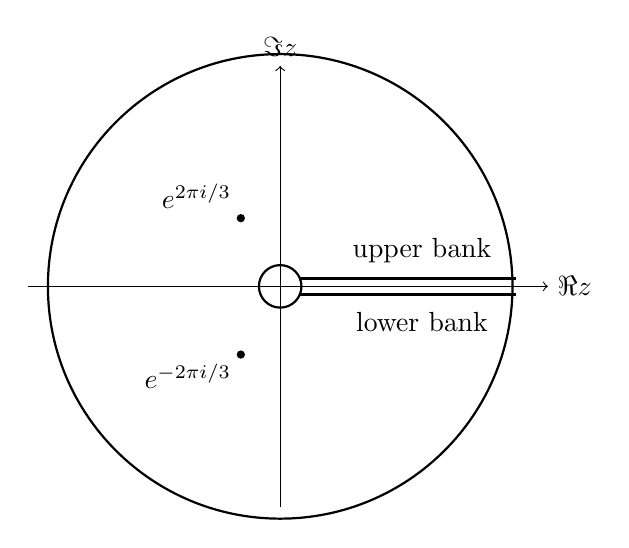
\begin{tikzpicture}[scale=1.0]
  \draw[->] (-3.2,0)--(3.4,0) node[right] {$\Re z$};
  \draw[->] (0,-2.8)--(0,2.8) node[above] {$\Im z$};
  \draw[very thick] (0.25,0.10)--(3.0,0.10);
  \draw[very thick] (3.0,-0.10)--(0.25,-0.10);
  \draw[thick] (0,0) circle (2.95);
  \draw[thick] (0,0) circle (0.27);
  \fill (-0.5,0.866) circle (1.5pt) node[above left] {$e^{2\pi i/3}$};
  \fill (-0.5,-0.866) circle (1.5pt) node[below left] {$e^{-2\pi i/3}$};
  \node at (1.8,0.45) {upper bank};
  \node at (1.8,-0.45) {lower bank};
\end{tikzpicture}
\caption{A keyhole contour compares the two boundary values of $z^\alpha$ across the cut and encloses the two zeros $e^{\pm2\pi i/3}$ of $z^2+z+1$, producing the Mellin-type evaluation.}
\label{fig:cp-iv-0063-mellin-keyhole-contour}
\end{figure}


\begin{solution}
Set
\[
I(\alpha)
=
\int_0^\infty
\frac{x^\alpha}{x^2+x+1}\,dx,
\qquad -1<\alpha<1.
\]
Use the standard Mellin integral
\[
\int_0^\infty
\frac{x^{\mu-1}}
{x^2+2x\cos\phi+1}\,dx
=
\frac{\pi\sin((1-\mu)\phi)}
{\sin(\pi\mu)\sin\phi},
\qquad
0<\mu<2.
\]
Here
\[
\mu=\alpha+1,
\qquad
\phi=\frac{\pi}{3},
\]
because
\[
x^2+x+1
=
x^2+2x\cos\frac{\pi}{3}+1.
\]
Therefore
\[
I(\alpha)
=
\frac{
\pi\sin(-\alpha\pi/3)
}{
\sin(\pi(\alpha+1))\sin(\pi/3)
}.
\]
Using
\[
\sin(\pi(\alpha+1))=-\sin(\pi\alpha),
\qquad
\sin\frac{\pi}{3}=\frac{\sqrt3}{2},
\]
we get
\[
\boxed{
I(\alpha)
=
\frac{2\pi}{\sqrt3}\,
\frac{\sin(\pi\alpha/3)}{\sin(\pi\alpha)},
\qquad -1<\alpha<1,\ \alpha\neq0.
}
\]

The singular-looking quotient has a removable limit at \(\alpha=0\):
\[
\lim_{\alpha\to0}I(\alpha)
=
\frac{2\pi}{3\sqrt3},
\]
which agrees directly with
\[
\int_0^\infty\frac{dx}{x^2+x+1}.
\]

Thus the migrated formula with \(\sin((\alpha+1)\pi/3)\) in the numerator is not consistent with the stated integral; the correct numerator is \(\sin(\pi\alpha/3)\).
\end{solution}


\begin{problem}[CP-IV-0064]
\label{prob:cp-iv-0064}
\par\noindent\textbullet\quad Does the conclusion still hold if we only assume $f_n \to f$ pointwise? Give a proof or counterexample.
\end{problem}

\begin{solution}
\par\medskip\noindent\textbf{(a) Uniform limits preserve uniform continuity.}\quad 
Fix $\varepsilon>0$. Choose $N$ so that $\|f_N-f\|_\infty<\varepsilon/3$ (uniform convergence).
Since $f_N$ is uniformly continuous, there exists $\delta>0$ such that
$|x-y|<\delta \implies |f_N(x)-f_N(y)|<\varepsilon/3$.
Then for all $x,y$ with $|x-y|<\delta$,
\[
|f(x)-f(y)|
\le |f(x)-f_N(x)| + |f_N(x)-f_N(y)| + |f_N(y)-f(y)|
< \varepsilon/3 + \varepsilon/3 + \varepsilon/3
= \varepsilon.
\]
Hence $f$ is uniformly continuous.

\par\medskip\noindent\textbf{(b) Pointwise convergence need not preserve uniform continuity.}\quad 
Consider $f_n(x)=\arctan(n x)$. Each $f_n$ is uniformly continuous (indeed $|f'_n(x)|=\frac{n}{1+n^2x^2}\le 1$).
Pointwise,
\[
f(x)=\lim_{n\to\infty} f_n(x)=
\begin{cases}
	\frac{\pi}{2}, & x>0,\\
	0, & x=0,\\
	-\frac{\pi}{2}, & x<0,
\end{cases}
\]
which is discontinuous at $0$, hence not uniformly continuous. Therefore pointwise convergence does not suffice.

\par\medskip\noindent\textbf{Examples.}\quad 
(1) $f_n(x)=\frac{x}{n+1}\to 0$ uniformly; $0$ is uniformly continuous. \quad
(2) $f_n(x)=\sqrt{x^2+\frac1n}\to |x|$ uniformly on $\mathbb{R}$; $|x|$ is uniformly continuous.
\end{solution}

\begin{problem}[CP-IV-0067]
\label{prob:cp-iv-0067}
\par\noindent\textbullet\quad Show that $C^k([a,b])$ is a complete metric space.
\end{problem}

\begin{solution}
Equip \(C^k([a,b])\) with the norm
\[
\|f\|_{C^k}
=
\sum_{j=0}^{k}\|f^{(j)}\|_\infty.
\]
Let \((f_n)\) be Cauchy in this norm. Then for each
\[
j=0,\ldots,k,
\]
the sequence \((f_n^{(j)})\) is Cauchy in
\[
C([a,b])
\]
with the sup norm. Since \(C([a,b])\) is complete, there exists a continuous function \(g_j\) such that
\[
f_n^{(j)}\longrightarrow g_j
\]
uniformly.

It remains to show that the limits are compatible as derivatives. We use the standard fact: if
\[
u_n\to u
\]
uniformly and
\[
u_n'\to v
\]
uniformly on \([a,b]\), then \(u\in C^1\) and \(u'=v\). Indeed,
\[
u_n(x)-u_n(a)
=
\int_a^x u_n'(t)\,dt.
\]
Passing to the limit uniformly gives
\[
u(x)-u(a)
=
\int_a^x v(t)\,dt,
\]
so \(u'=v\).

Apply this successively to
\[
f_n,\ f_n',\ldots,f_n^{(k-1)}.
\]
We obtain
\[
g_0'=g_1,\quad
g_1'=g_2,\quad\ldots,\quad
g_{k-1}'=g_k.
\]
Hence
\[
g_0\in C^k([a,b])
\]
and
\[
g_0^{(j)}=g_j.
\]
Finally,
\[
\|f_n-g_0\|_{C^k}
=
\sum_{j=0}^k
\|f_n^{(j)}-g_j\|_\infty
\longrightarrow0.
\]
Therefore \(C^k([a,b])\) is complete.
\end{solution}


\begin{problem}[CP-IV-0068]
\label{prob:cp-iv-0068}
Let $f(z)=z^{2}$ and $C$ any closed $C^{1}$ loop avoiding singularities (there are none). Then
\[
\oint_{C} z^{2}\,dz \;=\; 0.
\]
\end{problem}

\begin{solution}
The integrand has the entire primitive
\[
F(z)=\frac{z^3}{3},
\qquad
F'(z)=z^2.
\]
Therefore, for every closed \(C^1\) loop \(C\),
\[
\oint_C z^2\,dz
=
\oint_C F'(z)\,dz
=
0.
\]

Equivalently, Cauchy's theorem applies because \(z^2\) is entire. Hence
\[
\boxed{\oint_C z^2\,dz=0}.
\]
\end{solution}


\begin{problem}[CP-IV-0071]
\label{prob:cp-iv-0071}
\par\noindent\textbullet\quad $f_n(x)=x^{2n}$ on $X=(0,1)$.
\end{problem}

\begin{solution}
For
\[
f_n(x)=x^{2n},
\qquad 0<x<1,
\]
we have, for every fixed \(x\in(0,1)\),
\[
x^{2n}\longrightarrow0.
\]
Thus
\[
f_n\longrightarrow0
\]
pointwise on \(X=(0,1)\).

The convergence is not uniform. Indeed,
\[
\sup_{0<x<1}x^{2n}=1
\]
for every \(n\): the supremum is not attained, but values become arbitrarily close to \(1\) as \(x\to1^{-}\). Hence
\[
\|f_n\|_\infty=1
\]
for all \(n\), so
\[
\|f_n-0\|_\infty\nrightarrow0.
\]

Each individual \(f_n\) is uniformly continuous on \((0,1)\), since
\[
|f_n'(x)|=2n x^{2n-1}\le2n
\]
and therefore \(f_n\) is Lipschitz. Thus this is another example where pointwise convergence does not imply uniform convergence.
\end{solution}


\begin{problem}[CP-IV-0073]
\label{prob:cp-iv-0073}
\par\noindent (iii)\quad Explain why this does not contradict the Heine--Borel theorem.
\end{problem}

\begin{solution}
\par\medskip\noindent\textbf{(i) Total boundedness.}\quad 
Let $\varepsilon>0$ and choose $N\in\mathbb{N}$ with $1/N<\varepsilon$. Partition $[0,1]$ into $N$ subintervals
$[k/N,(k+1)/N]$ for $k=0,\dots,N-1$. Since $\mathbb{Q}$ is dense, pick $q_k\in\mathbb{Q}\cap(k/N,(k+1)/N)$.
Then every $x\in X$ lies in some $[k/N,(k+1)/N]$ and satisfies $|x-q_k|<1/N<\varepsilon$. Hence
\[
X\ \subset\ \bigcup_{k=0}^{N-1} B_X(q_k,\varepsilon),
\]
a finite $\varepsilon$-cover. Therefore $X$ is totally bounded.

\par\medskip\noindent\textbf{(ii) Non-compactness via an open cover.}\quad 
Fix an irrational $a\in(0,1)$ and define, for $n\in\mathbb{N}$,
\[
U_n = X \cap\Big( (-\infty,a-1/n)\ \cup\ (a+1/n,\infty)\Big).
\]
Each $U_n$ is open in the subspace $X$, and $\{U_n\}_{n\in\mathbb{N}}$ covers $X$:
for any $x\in X$ with $x\ne a$, choose $n>\frac1{|x-a|}$ so that $x\in U_n$.
No finite subfamily covers $X$: if $n_0$ is maximal among a finite selection, then rational points in
$X\cap(a-1/n_0,a+1/n_0)$ remain uncovered. Hence $X$ is not compact.

\emph{Sequential variant.} Choose a sequence $(x_k)\subset X$ with $x_k\to a$ (irrational).
Then $(x_k)$ has no convergent subsequence in $X$ (its only possible limit is $a\notin X$), so $X$ is not compact.

\par\medskip\noindent\textbf{(iii) Consistency with Heine--Borel.}\quad 
Heine--Borel states that a subset of $\mathbb{R}$ is compact iff it is closed and bounded.
The set $X$ is bounded but not closed (its closure is $[0,1]$), hence not compact. Moreover, in metric spaces,
compact $\iff$ complete and totally bounded; $X$ is totally bounded but not complete, so it is not compact.
Thus there is no contradiction.
\end{solution}

\begin{problem}[CP-IV-0074]
\label{prob:cp-iv-0074}
Calculate $\displaystyle \int_{\gamma} z\sin z\,dz$ where $\gamma$ is the straight line joining $0$ to $i$.
\end{problem}

\begin{solution}
Since $z\sin z$ is entire, the integral is path independent. An antiderivative is
\[
F(z)=\int z\sin z\,dz=-z\cos z+\sin z,
\]
because $F'(z)=-\cos z+z\sin z+\cos z=z\sin z$. Hence
\[
\int_{\gamma} z\sin z\,dz = F(i)-F(0)
= \big(\sin i - i\cos i\big)-0.
\]
Using $\sin i = i\sinh 1$ and $\cos i=\cosh 1$,
\[
\sin i - i\cos i = i(\sinh 1-\cosh 1) = -\,\frac{i}{e}.
\]
Therefore
\[
\boxed{\displaystyle \int_{\gamma} z\sin z\,dz = -\,\frac{i}{e}.}
\]
\end{solution}

\begin{problem}[CP-IV-0075]
\label{prob:cp-iv-0075}
\par\noindent\textbullet\quad \textbf{$(C^1,\|\cdot\|_\infty)$ is not complete.}

	Let $f_n(x)=\sqrt{x^2+\tfrac{1}{n}}$.
	Then $f_n\in C^\infty$ and $f_n\to |x|$ uniformly, but $|x|\notin C^1$.
	Thus $(C^1([0,1]),\|\cdot\|_\infty)$ is incomplete.

	\medskip
\end{problem}

\begin{solution}
The stated idea is correct after placing the corner inside the interval. On \([0,1]\), use
\[
f_n(x)
=
\sqrt{\left(x-\frac12\right)^2+\frac1n}.
\]
Then every \(f_n\in C^\infty([0,1])\).

For every \(x\),
\[
f_n(x)
\longrightarrow
\left|x-\frac12\right|.
\]
Moreover,
\[
0\le
\sqrt{u^2+\frac1n}-|u|
=
\frac{1/n}
{\sqrt{u^2+1/n}+|u|}
\le
\frac1{\sqrt n},
\]
so the convergence is uniform:
\[
\left\|
f_n-\left|\,\cdot-\frac12\right|
\right\|_\infty
\le
\frac1{\sqrt n}
\longrightarrow0.
\]

Thus \((f_n)\) is Cauchy in the sup norm. But its uniform limit
\[
f(x)=\left|x-\frac12\right|
\]
is not differentiable at \(x=1/2\), hence
\[
f\notin C^1([0,1]).
\]
Therefore
\[
\boxed{
(C^1([0,1]),\|\cdot\|_\infty)
\text{ is not complete}.
}
\]

The unshifted sequence \(\sqrt{x^2+1/n}\) would converge to \(|x|=x\) on \([0,1]\), which is \(C^1\); the shift to \(x=1/2\) is necessary for this interval.
\end{solution}


\begin{problem}[CP-IV-0078]
\label{prob:cp-iv-0078}
Define $f:\mathbb C\to\mathbb C$ by $f(0)=0$ and
\[
f(z)=\frac{(1+i)x^{3}-(1-i)y^{3}}{x^{2}+y^{2}},\qquad z=x+iy\ne0.
\]
Show that $f$ satisfies the Cauchy--Riemann equations at $0$ but is not differentiable there.
\end{problem}

\begin{solution}
Write
\[
(1+i)x^3-(1-i)y^3=(x^3-y^3)+i(x^3+y^3),
\]
so for $(x,y)\neq(0,0)$
\[
u(x,y)=\frac{x^3-y^3}{x^2+y^2},\qquad
v(x,y)=\frac{x^3+y^3}{x^2+y^2},
\]
and put $u(0,0)=v(0,0)=0$.

\emph{CR at $(0,0)$.}
Compute partials at the origin via limits along the axes:
\[
u_x(0,0)=\lim_{h\to0}\frac{u(h,0)-0}{h}
=\lim_{h\to0}\frac{h^3/h^2}{h}=1,\quad
u_y(0,0)=\lim_{k\to0}\frac{u(0,k)-0}{k}
=\lim_{k\to0}\frac{-k^3/k^2}{k}=-1,
\]
\[
v_x(0,0)=\lim_{h\to0}\frac{v(h,0)-0}{h}
=\lim_{h\to0}\frac{h^3/h^2}{h}=1,\quad
v_y(0,0)=\lim_{k\to0}\frac{v(0,k)-0}{k}
=\lim_{k\to0}\frac{k^3/k^2}{k}=1.
\]
Hence $u_x(0,0)=v_y(0,0)=1$ and $u_y(0,0)=-v_x(0,0)=-1$, so the Cauchy--Riemann equations hold at $0$.

\emph{Not differentiable at $0$.}
If $f$ were complex-differentiable at 0, then $f'(0)=u_x(0,0)+i v_x(0,0)=1+i$ and
$\displaystyle \lim_{z\to0}\frac{f(z)}{z}$ would exist and equal $1+i$.
However,
\[
\frac{f(x)}{x}\to 1+i\quad(y=0),\qquad
\frac{f(x+ix)}{x+ix}=\frac{i x}{x(1+i)}=\frac{1+i}{2}\quad(y=x),
\]
so the limit depends on the path. Therefore $f$ is not differentiable at $0$.
\end{solution}

\begin{problem}[CP-IV-0081]
\label{prob:cp-iv-0081}
\par\noindent\textbullet\quad (\textbf{Composition law})
	Let $T(z)=Az+B\bar z$ and $S(z)=Cz+D\bar z$. Show
	\[
	S\circ T(z)=(CA+D\overline{B})\,z\;+\;(CB+D\overline{A})\,\bar z.
	\]
	Deduce that the set of real-linear maps $\mathbb{C}\to\mathbb{C}$ is closed under composition, and $S\circ T$ is complex-linear iff $CB+D\overline{A}=0$.
	\emph{Solution.} Note $\overline{T(z)}=\overline{A}\bar z+\overline{B}z$ and compute
	$S(T(z))=C\,T(z)+D\,\overline{T(z)}$; read off the $z,\bar z$ coefficients.
\end{problem}

\begin{solution}
Let
\[
T(z)=Az+B\overline z,
\qquad
S(z)=Cz+D\overline z.
\]
Then
\[
\overline{T(z)}
=
\overline A\,\overline z+\overline B\,z.
\]
Therefore
\[
\begin{aligned}
(S\circ T)(z)
&=
C\,T(z)+D\,\overline{T(z)}\\
&=
C(Az+B\overline z)
+
D(\overline A\,\overline z+\overline B\,z)\\
&=
(CA+D\overline B)z
+
(CB+D\overline A)\overline z.
\end{aligned}
\]
Hence
\[
\boxed{
S\circ T(z)
=
(CA+D\overline B)z
+
(CB+D\overline A)\overline z.
}
\]

Thus the class of real-linear maps \(\mathbb C\to\mathbb C\) is closed under composition.

A real-linear map
\[
Ez+F\overline z
\]
is complex-linear exactly when \(F=0\). Consequently
\[
S\circ T
\]
is complex-linear exactly when
\[
\boxed{CB+D\overline A=0}.
\]
\end{solution}


\begin{problem}[CP-IV-0083]
\label{prob:cp-iv-0083}
a circle mapped to the real axis

As a concrete example, let $L$ be the unit circle
	\[
	L = \{ z\in\mathbb C : |z|=1 \},
	\]
	and choose three distinct points on $L$:
	\[
	a = 1,\qquad b=-1,\qquad c=i.
	\]
	Then the associated map
	\[
	\Phi(z) = \frac{(z-a)(c-b)}{(z-b)(c-a)}
	\]
	sends $L$ onto the real axis, with
	\[
	\Phi(a)=0,\qquad \Phi(b)=\infty,\qquad \Phi(c)=1.
	\]
	For $z$ not on $L$, the sign of $\Im \Phi(z)$ indicates on which side of
	the circle $L$ the point $z$ lies. One side of $L$ (for instance, the
	interior) is mapped to the upper half-plane $\Im w>0$, while the other
	side (the exterior) is mapped to the lower half-plane $\Im w<0$.

	Figure~\ref{fig:crossratio-z-plane} illustrates this: we show the circle
	$L$, the points $a,b,c$, and a cloud of sample points in the plane,
	distinguished according to the sign of $\Im\Phi(z)$. In
	Figure~\ref{fig:crossratio-w-plane}, we see their images under $\Phi$,
	which lie strictly above or below the real axis.
\end{problem}
\begin{figure}[ht]
  \centering
  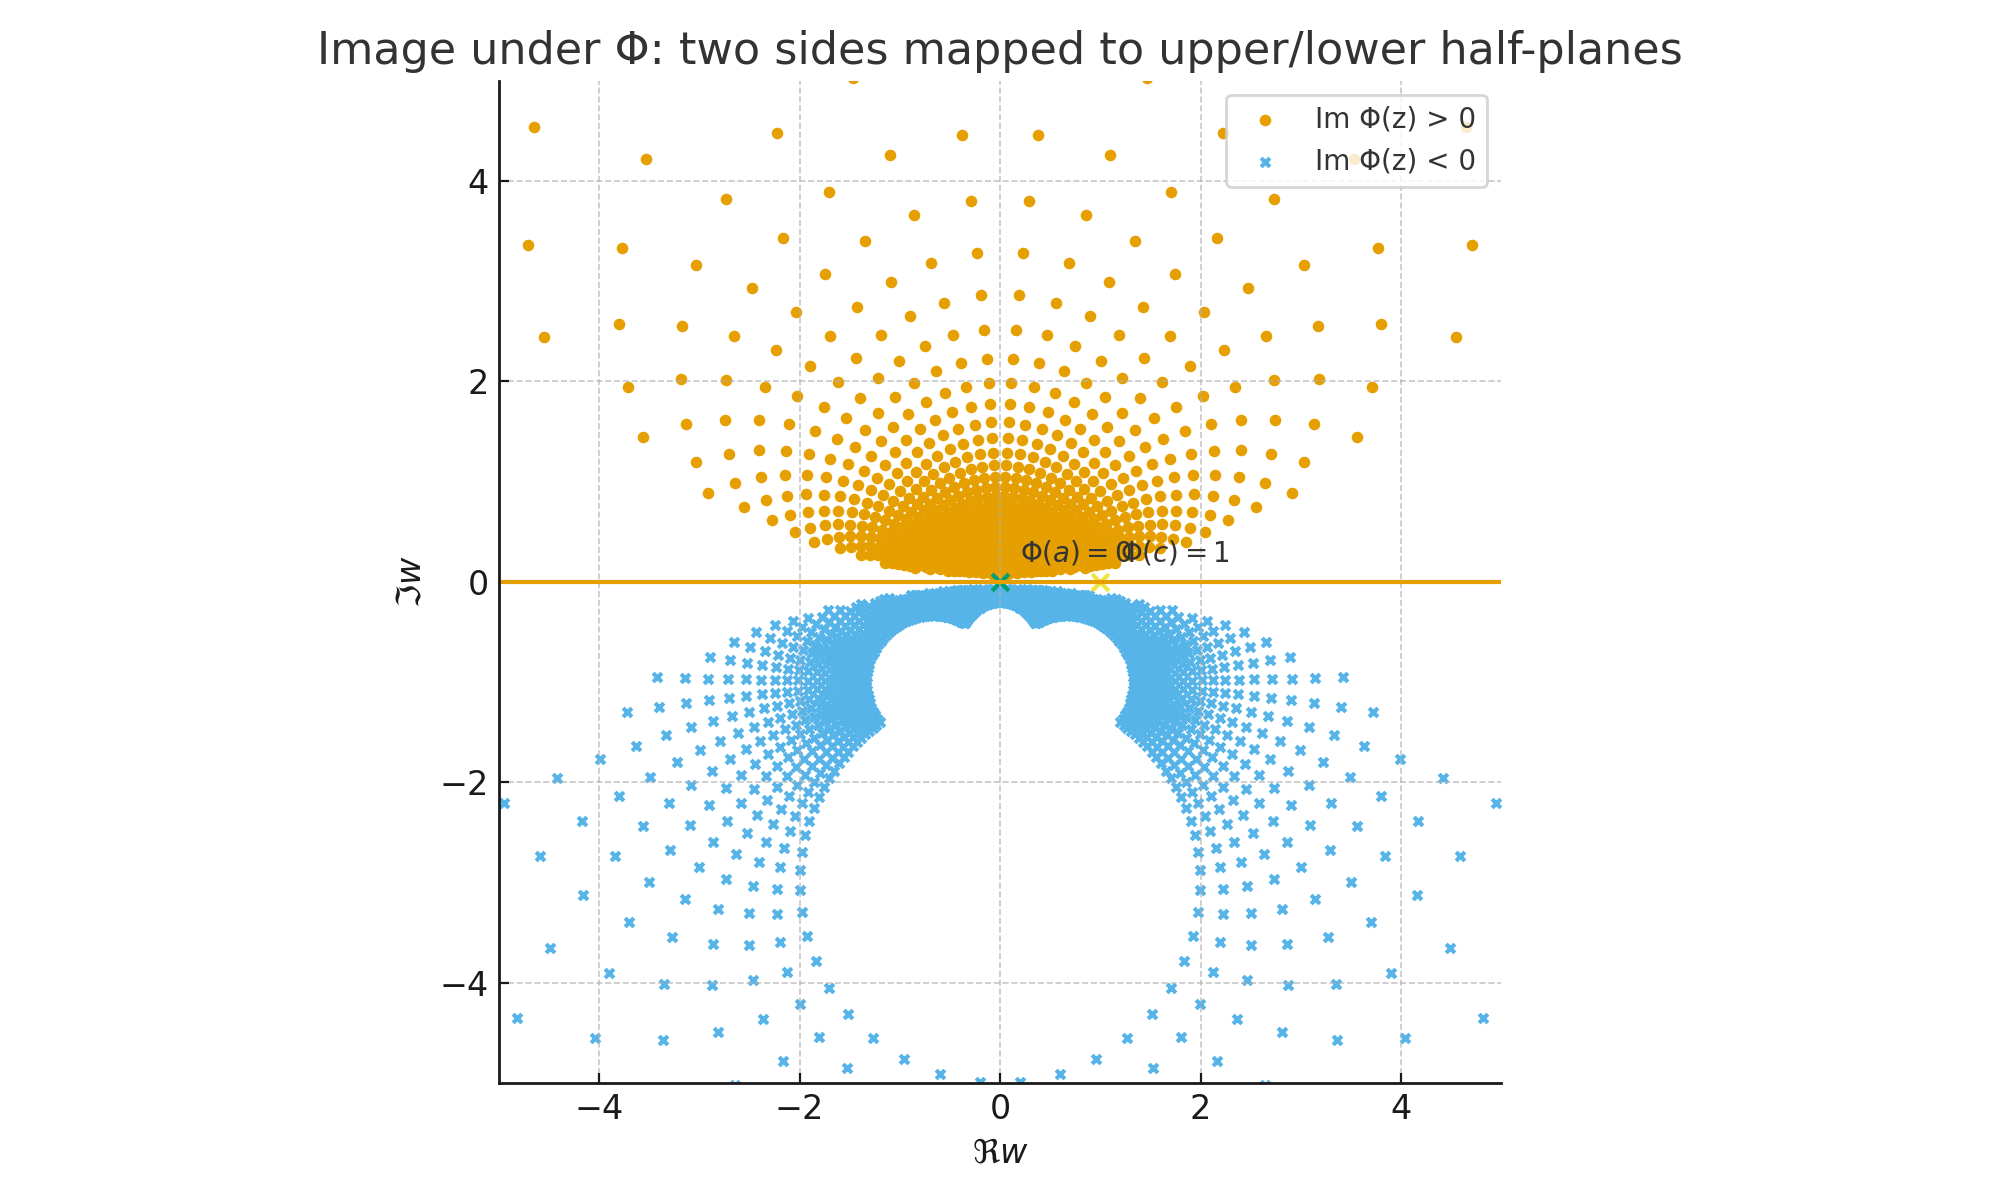
\includegraphics[width=0.78\textwidth]{figures/part04/cp_iv_0083_crossratio_circle_w_plane.png}
  \caption{Source-backed Part IV figure: crossratio w plane.}
  \label{fig:crossratio-w-plane}
\end{figure}

\begin{figure}[ht]
  \centering
  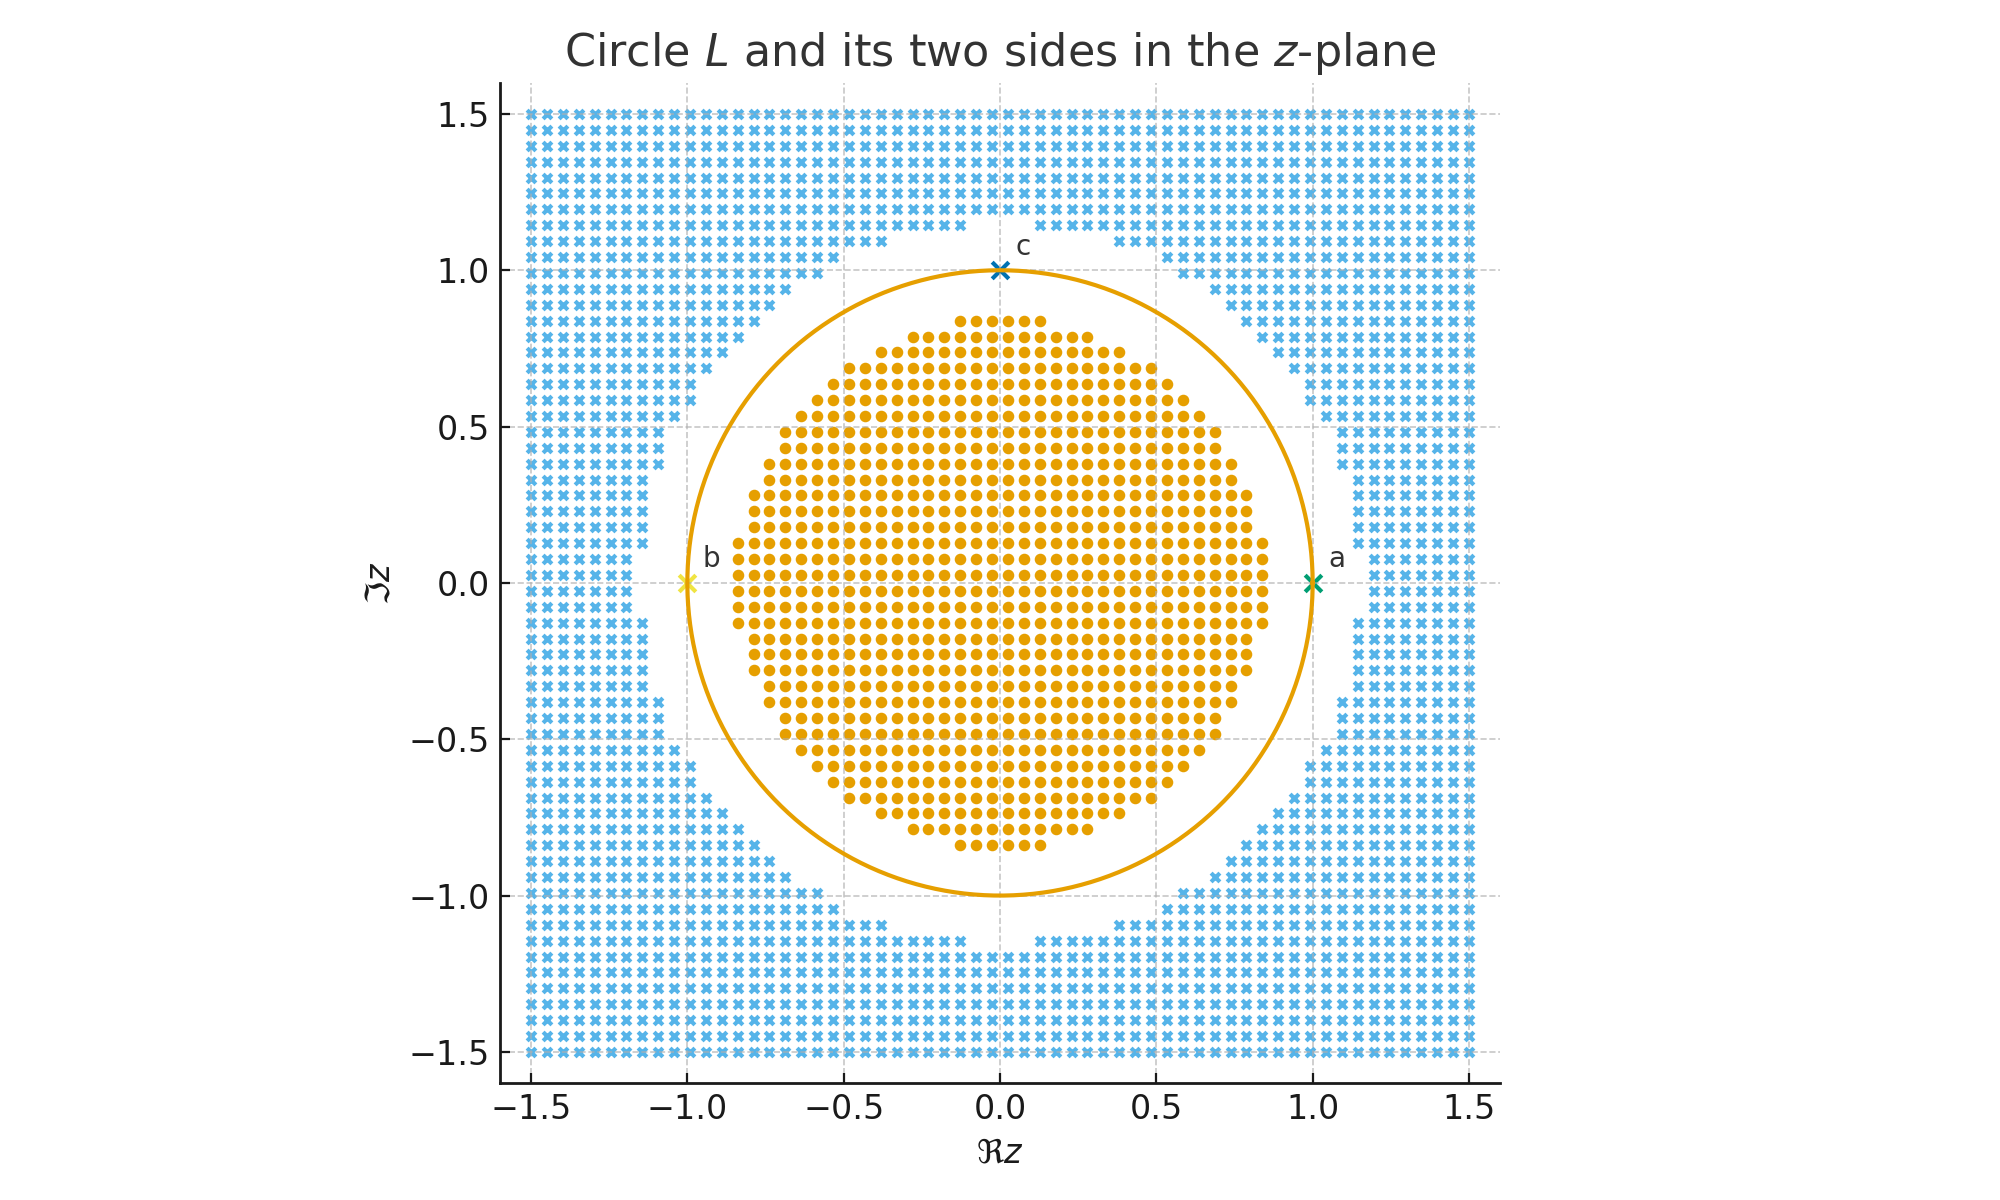
\includegraphics[width=0.78\textwidth]{figures/part04/cp_iv_0083_crossratio_circle_z_plane.png}
  \caption{Source-backed Part IV figure: crossratio z plane.}
  \label{fig:crossratio-z-plane}
\end{figure}

\begin{solution}
With
\[
a=1,\qquad b=-1,\qquad c=i,
\]
the cross-ratio map is
\[
\Phi(z)
=
\frac{(z-1)(i+1)}{(z+1)(i-1)}.
\]
Since
\[
\frac{1+i}{i-1}=-i,
\]
this simplifies to
\[
\boxed{
\Phi(z)
=
-i\,\frac{z-1}{z+1}.
}
\]
Directly,
\[
\Phi(1)=0,\qquad
\Phi(-1)=\infty,\qquad
\Phi(i)=1.
\]

A M\"obius transformation maps generalized circles to generalized circles. Since three distinct points of the unit circle are sent to
\[
0,\ \infty,\ 1\in\widehat{\mathbb R},
\]
the whole unit circle is sent to the extended real axis.

To determine the two sides, test one point from each component. The point \(z=0\) lies inside the unit disk and
\[
\Phi(0)=i,
\]
so
\[
|z|<1
\quad\Longrightarrow\quad
\Im\Phi(z)>0.
\]
For example, \(z=2\) lies outside the circle and
\[
\Phi(2)=-\frac{i}{3},
\]
so
\[
|z|>1
\quad\Longrightarrow\quad
\Im\Phi(z)<0.
\]

Therefore
\[
\boxed{
\Phi(\mathbb D)=\{\Im w>0\},
\qquad
\Phi(\widehat{\mathbb C}\setminus\overline{\mathbb D})
=
\{\Im w<0\}.
}
\]
This is exactly the side separation illustrated by the two referenced figures.
\end{solution}



\begin{problem}[CP-IV-0085]
\label{prob:cp-iv-0085}
\par\noindent\textbullet\quad $\{(x,0): 0< x< 1\}$.
\end{problem}

\begin{solution}
Let
\[
S=\{(x,0):0<x<1\}\subset\mathbb R^2.
\]
The set is not open in \(\mathbb R^2\), because every Euclidean ball centered at a point of \(S\) contains points with nonzero \(y\)-coordinate.

It is also not closed. For example,
\[
\left(\frac1n,0\right)\in S
\]
for \(n\ge2\), but
\[
\left(\frac1n,0\right)\longrightarrow(0,0)\notin S.
\]
Similarly, points of \(S\) approach \((1,0)\), which is not included.

Thus
\[
\boxed{
S\text{ is neither open nor closed in }\mathbb R^2.
}
\]
Its closure is the closed segment
\[
\overline S=\{(x,0):0\le x\le1\}.
\]
\end{solution}


\begin{problem}[CP-IV-0087]
\label{prob:cp-iv-0087}
\par\noindent\textbullet\quad $\{(x,y): y>0\}$.
\end{problem}

\begin{solution}
Let
\[
H=\{(x,y)\in\mathbb R^2:y>0\}.
\]
This is open because it is the inverse image
\[
H=\pi_2^{-1}((0,\infty))
\]
under the continuous projection
\[
\pi_2(x,y)=y.
\]

It is not closed. For instance,
\[
(0,1/n)\in H
\]
for every \(n\), but
\[
(0,1/n)\longrightarrow(0,0)\notin H.
\]
Hence
\[
\boxed{
H\text{ is open and not closed}.
}
\]
Its closure is
\[
\overline H=\{(x,y):y\ge0\}.
\]
\end{solution}


\begin{problem}[CP-IV-0088]
\label{prob:cp-iv-0088}
\par\noindent (i)\quad Show that $X$ is totally bounded.
\end{problem}

\begin{solution}
For the set \(X=\mathbb Q\cap[0,1]\) occurring in the surrounding exercise, let
\(\varepsilon>0\). Choose \(N\in\mathbb N\) such that
\[
\frac1N<\varepsilon.
\]
Partition \([0,1]\) into the \(N\) intervals
\[
I_k=\left[\frac{k}{N},\frac{k+1}{N}\right],
\qquad k=0,\ldots,N-1.
\]
Because \(\mathbb Q\) is dense in \(\mathbb R\), choose
\[
q_k\in \mathbb Q\cap I_k
\]
for every \(k\).

If \(x\in X\), then \(x\in I_k\) for some \(k\), and therefore
\[
|x-q_k|\le \frac1N<\varepsilon.
\]
Hence
\[
X\subset
\bigcup_{k=0}^{N-1}B_X(q_k,\varepsilon).
\]
This is a finite \(\varepsilon\)-cover of \(X\). Since \(\varepsilon>0\) was arbitrary,
\[
\boxed{X\text{ is totally bounded}.}
\]
\end{solution}


\begin{problem}[CP-IV-0091]
\label{prob:cp-iv-0091}
— constant curl, easy numbers

Take $\mathbf F=(-y,x)$. Then $L=-y$, $M=x$ and
\[
M_x - L_y \;=\; \partial_x(x) - \partial_y(-y) \;=\; 1 - (-1) \;=\; 2 \quad(\text{constant}).
\]
Area integral:
\[
\iint_{D} (M_x-L_y)\,dA
\;=\;
\iint_{D} 2\,dA
\;=\; 2\,\pi R^2.
\]
Line integral (check by parametrizing $C$):
\[
dx=-R\sin t\,dt,\qquad dy=R\cos t\,dt,
\]
\[
L\,dx+M\,dy
=
(-y)\,dx + (x)\,dy
=
(-R\sin t)(-R\sin t)\,dt + (R\cos t)(R\cos t)\,dt
=
R^2\,dt,
\]
\[
\oint_{C} (L\,dx+M\,dy)
=
\int_{0}^{2\pi} R^2\,dt
=
2\pi R^2.
\]
Both sides match: $2\pi R^2$.
\end{problem}

\begin{solution}
Let
\[
\mathbf F=(L,M)=(-y,x)
\]
and let \(C=\partial D\) be the positively oriented circle
\[
x^2+y^2=R^2.
\]
Then
\[
M_x-L_y
=
\partial_x(x)-\partial_y(-y)
=
1-(-1)
=
2.
\]
Green's theorem therefore gives
\[
\oint_C(L\,dx+M\,dy)
=
\iint_D(M_x-L_y)\,dA
=
2\,\operatorname{Area}(D)
=
2\pi R^2.
\]

Directly, parametrize
\[
x=R\cos t,\qquad y=R\sin t,\qquad 0\le t\le2\pi.
\]
Then
\[
dx=-R\sin t\,dt,\qquad dy=R\cos t\,dt,
\]
so
\[
\begin{aligned}
L\,dx+M\,dy
&=
(-R\sin t)(-R\sin t)\,dt
+
(R\cos t)(R\cos t)\,dt\\
&=
R^2\,dt.
\end{aligned}
\]
Hence
\[
\oint_C(L\,dx+M\,dy)
=
\int_0^{2\pi}R^2\,dt
=
\boxed{2\pi R^2},
\]
in agreement with Green's theorem.
\end{solution}


\begin{problem}[CP-IV-0093]
\label{prob:cp-iv-0093}
\par\noindent\textbullet\quad (\textbf{Operator norm and singular values})
	Show the maximal and minimal stretch factors (singular values) of $T$ are
	\[
	\sigma_{\max}=|A|+|B|,\qquad \sigma_{\min}=\bigl||A|-|B|\bigr|.
	\]
	\emph{Solution (sketch).} Write $T(z)=A\bigl(z+\tfrac{B}{A}\bar z\bigr)$ if $A\neq0$; by rotating/scaling the domain and range one reduces to $A\ge0$, $B\ge0$ real. Then $T$ acts by stretching along two orthogonal directions with factors $A\pm B$, giving the claim. General case follows by unitary conjugation.
\end{problem}

\begin{solution}
Let
\[
T(z)=Az+B\overline z.
\]
Multiplying the domain and range by complex numbers of modulus \(1\) does not change
singular values. Hence, after rotations, we may reduce to
\[
A=a\ge0,\qquad B=b\ge0.
\]
Writing \(z=x+iy\),
\[
T(z)
=
a(x+iy)+b(x-iy)
=
(a+b)x+i(a-b)y.
\]
Thus, in suitable orthonormal coordinates, the real matrix is diagonal:
\[
\begin{pmatrix}
a+b&0\\
0&a-b
\end{pmatrix}.
\]
The stretch factors along the two orthogonal principal directions are therefore
\[
|a+b|
\quad\text{and}\quad
|a-b|.
\]
Undoing the rotations gives
\[
\boxed{
\sigma_{\max}=|A|+|B|,
\qquad
\sigma_{\min}=\bigl||A|-|B|\bigr|.
}
\]

In particular,
\[
T\text{ is invertible}
\iff
\sigma_{\min}>0
\iff
|A|\neq|B|,
\]
and its real Jacobian is
\[
\det_{\mathbb R}T
=
(|A|+|B|)(|A|-|B|)
=
|A|^2-|B|^2.
\]
\end{solution}


\begin{problem}[CP-IV-0094]
\label{prob:cp-iv-0094}
\par\noindent\textbullet\quad \textbf{Derivative not continuous from $(C^1,\|\cdot\|_\infty)$ to $(C,\|\cdot\|_\infty)$.}

	Take $f_n(x)=\tfrac{1}{n}\sin(n^2 x)$ on $[0,1]$.
	We have
	\[
	\|f_n\|_\infty=\frac{1}{n}\longrightarrow 0,
	\qquad
	\|f_n'\|_\infty = n \longrightarrow \infty .
	\]
	Hence $D$ is discontinuous with these norms.

	\medskip
\end{problem}

\begin{solution}
Consider the differentiation operator
\[
D:(C^1([0,1]),\|\cdot\|_\infty)
\longrightarrow
(C([0,1]),\|\cdot\|_\infty),
\qquad
Df=f'.
\]
Take
\[
f_n(x)=\frac1n\sin(n^2x).
\]
Then
\[
\|f_n\|_\infty\le\frac1n\longrightarrow0,
\]
so \(f_n\to0\) in the norm of the domain.

However,
\[
f_n'(x)=n\cos(n^2x),
\]
and hence
\[
\|Df_n-D0\|_\infty
=
\|f_n'\|_\infty
=
n\longrightarrow\infty.
\]
Thus \(f_n\to0\) in the domain while \(Df_n\not\to0\) in the codomain. Therefore
\[
\boxed{D\text{ is not continuous for these norms}.}
\]
\end{solution}


\begin{problem}[CP-IV-0095]
\label{prob:cp-iv-0095}
$|x|^3$ is $C^2$ with
$f'(x)=3x^2$ for $x>0$ and $f'(x)=-3x^2$ for $x<0$,
$f''(x)=6x$ for $x>0$ and $f''(x)=-6x$ for $x<0$, both extending continuously at $0$ by $0$,
while $f^{(3)}(x)=6$ for $x>0$ and $f^{(3)}(x)=-6$ for $x<0$, so $f^{(3)}$ has a jump at $0$.
\end{problem}

\begin{solution}
Let
\[
f(x)=|x|^3.
\]
For \(x>0\),
\[
f(x)=x^3,
\]
whereas for \(x<0\),
\[
f(x)=-x^3.
\]
Thus
\[
f'(x)=
\begin{cases}
3x^2,&x>0,\\
-3x^2,&x<0,
\end{cases}
\qquad
f'(0)=0,
\]
so \(f'\) is continuous at \(0\).

Differentiating again,
\[
f''(x)=
\begin{cases}
6x,&x>0,\\
-6x,&x<0,
\end{cases}
=
6|x|
\quad(x\neq0),
\]
and \(f''(0)=0\). Hence \(f''\) is continuous at \(0\), so
\[
f\in C^2(\mathbb R).
\]

For \(x\neq0\),
\[
f'''(x)=
\begin{cases}
6,&x>0,\\
-6,&x<0.
\end{cases}
\]
The one-sided limits at \(0\) are different, so \(f'''(0)\) does not exist. Therefore
\[
\boxed{|x|^3\in C^2(\mathbb R)\setminus C^3(\mathbb R).}
\]
\end{solution}


\begin{problem}[CP-IV-0100]
\label{prob:cp-iv-0100}
\par\noindent\textbullet\quad \textbf{Integration map is Lipschitz $C^k\!\to C^{k+1}$.}

	For $f,g\in C^k$ put $F=T(f)$ and $G=T(g)$ with
	\[
	F(x)=\int_a^x f(y)\,dy, \qquad G(x)=\int_a^x g(y)\,dy .
	\]
	Then
	\[
	\|F-G\|_\infty \;\le\; (b-a)\,\|f-g\|_\infty,
	\]
	and for $1\le j\le k+1$,
	\[
	\|F^{(j)}-G^{(j)}\|_\infty \;=\; \|f^{(j-1)}-g^{(j-1)}\|_\infty .
	\]
	Consequently,
	\[
	d_{C^{k+1}}(T(f),T(g))
	\;\le\; \max\{1,b-a\}\; d_{C^k}(f,g).
	\]

	\medskip
\end{problem}

\begin{solution}
Let
\[
T(f)(x)=\int_a^x f(y)\,dy.
\]
For \(f,g\in C^k([a,b])\), set \(h=f-g\). Then
\[
|T(f)(x)-T(g)(x)|
=
\left|\int_a^x h(y)\,dy\right|
\le
(b-a)\|h\|_\infty,
\]
and therefore
\[
\|T(f)-T(g)\|_\infty
\le
(b-a)\|f-g\|_\infty.
\]
Moreover, for \(1\le j\le k+1\),
\[
(Tf)^{(j)}=f^{(j-1)},
\]
so
\[
\|(Tf)^{(j)}-(Tg)^{(j)}\|_\infty
=
\|f^{(j-1)}-g^{(j-1)}\|_\infty.
\]

With the sum metric
\[
d_{C^k}(f,g)
=
\sum_{j=0}^{k}\|f^{(j)}-g^{(j)}\|_\infty,
\]
we obtain
\[
\begin{aligned}
d_{C^{k+1}}(Tf,Tg)
&\le
(b-a)\|f-g\|_\infty+d_{C^k}(f,g)\\
&\le
\bigl(1+b-a\bigr)d_{C^k}(f,g).
\end{aligned}
\]
Hence \(T:C^k\to C^{k+1}\) is Lipschitz, and therefore continuous.

If instead one uses the maximum norm
\[
\|f\|_{C^k,\max}
=
\max_{0\le j\le k}\|f^{(j)}\|_\infty,
\]
then the sharper constant stated in the migrated text is valid:
\[
\boxed{
\|Tf-Tg\|_{C^{k+1},\max}
\le
\max\{1,b-a\}\,
\|f-g\|_{C^k,\max}.
}
\]
Thus the printed constant depends on which standard \(C^k\) metric is being used.
\end{solution}


\begin{problem}[CP-IV-0101]
\label{prob:cp-iv-0101}
\par\noindent\textbullet\quad (\textbf{Wirtinger derivatives})
	For $T(z)=Az+B\bar z$, compute $\partial T/\partial z$ and $\partial T/\partial\bar z$.
	\emph{Solution.} $\displaystyle \frac{\partial T}{\partial z}=A,\qquad \frac{\partial T}{\partial\bar z}=B$.
\end{problem}

\begin{solution}
Using the Wirtinger operators
\[
\frac{\partial}{\partial z}
=
\frac12\left(
\frac{\partial}{\partial x}
-i\frac{\partial}{\partial y}
\right),
\qquad
\frac{\partial}{\partial\overline z}
=
\frac12\left(
\frac{\partial}{\partial x}
+i\frac{\partial}{\partial y}
\right),
\]
we have
\[
\frac{\partial z}{\partial z}=1,
\qquad
\frac{\partial\overline z}{\partial z}=0,
\]
and
\[
\frac{\partial z}{\partial\overline z}=0,
\qquad
\frac{\partial\overline z}{\partial\overline z}=1.
\]
Therefore, for
\[
T(z)=Az+B\overline z,
\]
\[
\boxed{
\frac{\partial T}{\partial z}=A,
\qquad
\frac{\partial T}{\partial\overline z}=B.
}
\]
In particular, the Cauchy--Riemann condition is
\[
\frac{\partial T}{\partial\overline z}=0,
\]
so \(T\) is holomorphic exactly when \(B=0\).
\end{solution}


\begin{problem}[CP-IV-0103]
\label{prob:cp-iv-0103}
\par\noindent\textbullet\quad (\textbf{Matrix from $A,B$})
	Given $T(z)=Az+B\bar z$ with $A=\alpha+i\beta$, $B=\gamma+i\delta$ ($\alpha,\beta,\gamma,\delta\in\mathbb{R}$), show the real matrix is
	\[
	\begin{pmatrix}
		\alpha+\gamma & -\beta+\delta\\
		\beta+\delta & \alpha-\gamma
	\end{pmatrix}.
	\]
	\emph{Solution.} Expand $Az+B\bar z$ with $z=x+iy$ and collect $(x,y)$ coefficients.
\end{problem}

\begin{solution}
Let
\[
A=\alpha+i\beta,
\qquad
B=\gamma+i\delta,
\qquad
z=x+iy.
\]
Then
\[
\begin{aligned}
Az
&=
(\alpha x-\beta y)+i(\beta x+\alpha y),\\
B\overline z
&=
(\gamma x+\delta y)+i(\delta x-\gamma y).
\end{aligned}
\]
Adding,
\[
T(z)
=
\bigl((\alpha+\gamma)x+(-\beta+\delta)y\bigr)
+
i\bigl((\beta+\delta)x+(\alpha-\gamma)y\bigr).
\]
Hence the real matrix of \(T\) in the basis \((1,i)\) is
\[
\boxed{
\begin{pmatrix}
\alpha+\gamma&-\beta+\delta\\
\beta+\delta&\alpha-\gamma
\end{pmatrix}.
}
\]
\end{solution}


\begin{problem}[CP-IV-0104]
\label{prob:cp-iv-0104}
\par\noindent\textbullet\quad $B=\{f\in C([0,1]) : \int_0^1 f=0\}$.

Does the answer change if we replace $d_\infty$ with the $L^1$ metric $d_1(f,g)=\int_0^1 |f-g|$?
\end{problem}

\begin{solution}
\par\medskip\noindent\textbf{Uniform (sup) metric.}\quad 

	\par\noindent (a)\quad $A$ is \emph{closed} and not open. The evaluation map $\mathrm{ev}_{1/2}:f\mapsto f(1/2)$ is continuous on $(C([0,1]),\|\cdot\|_\infty)$, hence $A=\mathrm{ev}_{1/2}^{-1}(\{0\})$ is closed. It is not open: for any $f\in A$ and $\varepsilon>0$, add a small continuous bump supported near $1/2$ to obtain $g$ with $\|g-f\|_\infty<\varepsilon$ but $g(1/2)\ne 0$.
	\par\noindent (b)\quad $B$ is \emph{closed} and not open. The functional $I(f)=\int_0^1 f$ is continuous since $|I(f)-I(g)|\le \int_0^1 |f-g|\le \|f-g\|_\infty$. Thus $B=I^{-1}(\{0\})$ is closed. It is not open: perturb $f$ by a small positive (or negative) bump of arbitrarily small height/support to change the integral while keeping $\|\,\cdot\,\|_\infty$ small.

\par\medskip\noindent\textbf{$L^1$ metric.}\quad 

	\par\noindent (a)\quad $A$ is \emph{neither open nor closed}. Evaluation at a point is not continuous in $L^1$.

		\par\noindent\textbullet\quad Not closed: let $g\equiv 1$, and let $f_n$ be continuous functions with $f_n(1/2)=0$ and $f_n\equiv 1$ outside $(\tfrac12-\tfrac1n,\tfrac12+\tfrac1n)$ (linear ramps in between). Then $f_n\in A$ and $\int_0^1|f_n-g|\le 2/n\to0$, so $f_n\to g$ in $L^1$ with $g\notin A$.
		\par\noindent\textbullet\quad Not open: given $f\in A$ and $\varepsilon>0$, add a very narrow spike near $1/2$ (choose height/width so its area $<\varepsilon$) producing $h$ with $d_1(h,f)<\varepsilon$ but $h(1/2)\ne 0$.

	\par\noindent (b)\quad $B$ is \emph{closed} and not open. The map $I(f)=\int_0^1 f$ is continuous in $L^1$ because $|I(f)-I(g)|\le \int_0^1|f-g|$. Hence $B=I^{-1}(\{0\})$ is closed. As before, small-area bumps show $B$ is not open.

\par\medskip\noindent\textbf{Summary.}\quad 
Under $d_\infty$: $A$ closed/not open; $B$ closed/not open.
Under $d_1$: $A$ neither open nor closed; $B$ closed/not open.
\end{solution}

\begin{problem}[CP-IV-0105]
\label{prob:cp-iv-0105}
Show that the following functions do not have antiderivatives on the indicated domains:
\[
\text{(a)}\; f(z)=\frac{1}{z}-\frac{1}{z-1}\quad\text{on } \{\,0<|z|<1\,\},\qquad
\text{(b)}\; g(z)=\frac{z}{1+z^{2}}\quad\text{on } \{\,1<|z|<\infty\,\}.
\]
\end{problem}

\begin{solution}
A holomorphic function with an antiderivative has integral \(0\) around every closed curve.

For
\[
f(z)=\frac1z-\frac1{z-1}
\]
on
\[
D_1=\{0<|z|<1\},
\]
choose the positively oriented circle
\[
\gamma(t)=re^{it},
\qquad 0<r<1.
\]
The term \(1/(z-1)\) is holomorphic inside this circle, while \(1/z\) has residue \(1\) at \(0\). Hence
\[
\oint_\gamma f(z)\,dz
=
2\pi i\neq0.
\]
Therefore \(f\) has no antiderivative on \(D_1\).

For
\[
g(z)=\frac{z}{1+z^2}
\]
on
\[
D_2=\{|z|>1\},
\]
choose the circle \(|z|=R\) with \(R>1\). The poles \(i\) and \(-i\) lie inside it, and
\[
\operatorname{Res}(g;i)
=
\frac12,
\qquad
\operatorname{Res}(g;-i)
=
\frac12.
\]
Thus
\[
\oint_{|z|=R}g(z)\,dz
=
2\pi i\left(\frac12+\frac12\right)
=
2\pi i\neq0.
\]
The contour itself lies entirely in \(D_2\). Hence \(g\) also has no antiderivative on its stated domain.
\end{solution}


\begin{problem}[CP-IV-0108]
\label{prob:cp-iv-0108}
Let $T:\mathbb{R}^2\to\mathbb{R}^2$ be a real-linear map. Regard $T$ as a map $\mathbb{C}\to\mathbb{C}$ via $(x,y)\leftrightarrow x+iy$.
	Show that there exist unique $A,B\in\mathbb{C}$ such that
	\[
	T(z)=Az+B\overline{z}\qquad(\forall\,z\in\mathbb{C}),
	\]
	and that $T$ is complex differentiable (i.e.\ $\mathbb{C}$-linear) iff $B=0$.
\end{problem}

\begin{solution}
Let
\[
T(x+iy)=(ax+by)+i(cx+dy)
\]
be a real-linear map. Define
\[
A=\frac{a+d}{2}+i\,\frac{c-b}{2},
\qquad
B=\frac{a-d}{2}+i\,\frac{c+b}{2}.
\]
A direct expansion gives
\[
Az+B\overline z
=
(ax+by)+i(cx+dy)
=
T(z),
\]
so such \(A,B\) exist.

They are unique. Indeed, if
\[
Az+B\overline z
=
A'z+B'\overline z
\]
for every \(z\), then evaluating at \(z=1\) and \(z=i\) gives
\[
A+B=A'+B',
\qquad
A-B=A'-B',
\]
hence
\[
A=A',
\qquad
B=B'.
\]

Finally, a real-linear map is complex-linear exactly when
\[
T(iz)=iT(z)
\]
for every \(z\). From
\[
T(z)=Az+B\overline z
\]
we get
\[
T(iz)=iAz-iB\overline z,
\]
whereas
\[
iT(z)=iAz+iB\overline z.
\]
Thus these are equal for all \(z\) exactly when
\[
B=0.
\]
Therefore
\[
\boxed{
T\text{ is complex-linear (equivalently holomorphic) iff }B=0.
}
\]
\end{solution}


\begin{problem}[CP-IV-0109]
\label{prob:cp-iv-0109}
\par\noindent\textbullet\quad $U=\displaystyle\bigcup_{n=1}^{\infty}(-n,\sin n)$.
\end{problem}

\begin{solution}
\par\medskip\noindent\textbf{Background (subspace).}\quad 
If $Y\subset\mathbb{R}$ has the subspace metric, then $A\subset Y$ is open in $Y$ iff $A=Y\cap O$ for some open $O\subset\mathbb{R}$, and $A$ is closed in $Y$ iff $A=Y\cap F$ for some closed $F\subset\mathbb{R}$.

\par\medskip\noindent\textbf{(a) $U=(0,1)\cup(2,3)$ in $\mathbb{R}$.}\quad 
$U$ is a union of open intervals $\Rightarrow$ \emph{open}.
It is \emph{not closed} since $1$ and $2$ are limit points not in $U$.

\par\medskip\noindent\textbf{(b) $U=[0,1]$ under different ambients.}\quad 

	\par\noindent\textbullet\quad In $\mathbb{R}$: $U$ is \emph{closed} (complement open), \emph{not open}.
	\par\noindent\textbullet\quad In $[-1,1]$: $U=[-1,1]\cap(-\infty,1]$ $\Rightarrow$ \emph{closed}; \emph{not open} (any subspace ball at $0$ contains negatives).
	\par\noindent\textbullet\quad In $(0,1)$: $U=[0,1]\cap(0,1)=(0,1)$ equals the whole space $\Rightarrow$ \emph{open and closed}.
	\par\noindent\textbullet\quad In $[0,2]$: $U=[0,2]\cap(-\infty,1]$ $\Rightarrow$ \emph{closed}; \emph{not open} (neighborhoods of $1$ include points $>1$).

\par\medskip\noindent\textbf{(c) $U=\displaystyle\bigcup_{n=1}^{\infty}(-n,\sin n)$ in $\mathbb{R}$.}\quad 
Each $(-n,\sin n)$ is open, so $U$ is \emph{open}.
Since $\{\sin n:n\in\mathbb{N}\}$ is dense in $[-1,1]$, every $y<1$ lies in some $(-n,\sin n)$, while $1\notin U$. Hence
\[
U=(-\infty,1),
\]
which is \emph{open} and \emph{not closed} (its closure is $(-\infty,1]$).
\end{solution}

\begin{problem}[CP-IV-0113]
\label{prob:cp-iv-0113}
Let $(X,d)$ be a metric space and $\{x_n\}_{n=1}^\infty\subset X$. We say $x_n\to x\in X$ if
\[
(\ast)\qquad \forall \varepsilon>0\ \exists N(\varepsilon)\in\mathbb{N}\ \text{ such that }\ d(x_n,x)<\varepsilon\ \text{ for all } n\ge N(\varepsilon).
\]

\par\noindent (a)\quad Show that $x_n\to x$ is equivalent to:
\[
(\ast\ast)\qquad \forall V\subset X\ \text{with }V\text{ a neighborhood of }x,\ \exists N(V)\ \text{ such that } x_n\in V\ \text{ for all } n\ge N(V).
\]
\par\noindent (b)\quad Using $(\ast)$, prove that if $\{x_n\}$ converges in $X$, then its limit is unique.

A set $V\subset X$ is a neighborhood of $x$ if there exists $r>0$ with the open ball $B(x,r)=\{y\in X: d(x,y)<r\}$ contained in $V$. The triangle inequality states $d(x,y)\le d(x,z)+d(z,y)$, and $d(x,y)=0$ implies $x=y$.
\end{problem}

\begin{solution}
\emph{($\ast\Rightarrow\ast\ast$)} Let $V$ be a neighborhood of $x$. Then $\exists r>0$ with $B(x,r)\subset V$. By $(\ast)$ with $\varepsilon=r$, there is $N(r)$ such that $d(x_n,x)<r$ for all $n\ge N(r)$, hence $x_n\in B(x,r)\subset V$. Set $N(V):=N(r)$.

\smallskip
\noindent
\emph{($\ast\ast\Rightarrow\ast$)} Fix $\varepsilon>0$. The ball $B(x,\varepsilon)$ is a neighborhood of $x$, so by $(\ast\ast)$ there exists $N$ with $x_n\in B(x,\varepsilon)$ for all $n\ge N$, i.e.\ $d(x_n,x)<\varepsilon$. Thus $(\ast)$ holds.
\end{solution}

\begin{problem}[CP-IV-0114]
\label{prob:cp-iv-0114}
Let $f(z)=e^{-z^{2}}$. Using an appropriate contour and the Cauchy--Goursat theorem, show that for $b>0$,
	\[
	\int_{0}^{\infty} e^{-x^{2}}\cos(2bx)\,dx=\frac{\sqrt{\pi}}{2}\,e^{-b^{2}}.
	\]
	You may use $\int_{0}^{\infty} e^{-x^{2}}\,dx=\sqrt{\pi}/2$.
\end{problem}

% Designed Companion Part IV figure
% Intended for \input{...} beside the matching canonical problem.
\begin{figure}[ht]
\centering
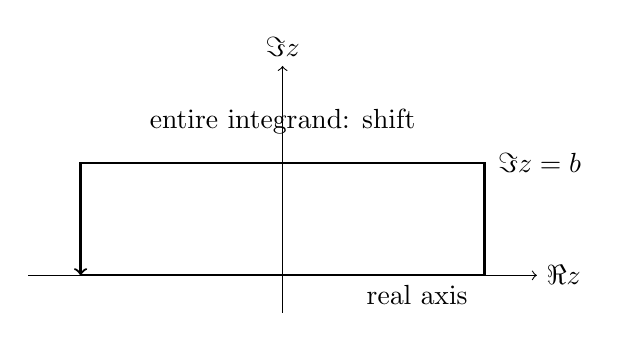
\begin{tikzpicture}[scale=0.95]
  \draw[->] (-3.4,0)--(3.4,0) node[right] {$\Re z$};
  \draw[->] (0,-0.5)--(0,2.8) node[above] {$\Im z$};
  \draw[thick,->] (-2.7,0)--(2.7,0)--(2.7,1.5)--(-2.7,1.5)--(-2.7,0);
  \node[right] at (2.75,1.5) {$\Im z=b$};
  \node[below] at (1.8,0) {real axis};
  \node at (0,2.05) {entire integrand: shift};
\end{tikzpicture}
\caption{Completing the square converts the oscillatory Gaussian to a vertically shifted Gaussian. Because the integrand is entire and decays on the vertical sides, Cauchy--Goursat shifts the real line to $\Im z=b$.}
\label{fig:cp-iv-0114-gaussian-shift-rectangle}
\end{figure}


\begin{solution}
\noindent\textbf{Step 1: The rectangle.}\;
	Consider the rectangle with vertices $-R,\,R,\,R+ib,\,-R+ib$ oriented counterclockwise.
	Since $e^{-z^{2}}$ is entire, Cauchy--Goursat gives
	\[
	\int_{-R}^{R} e^{-x^{2}}\,dx
	+\int_{\text{right}} e^{-z^{2}}\,dz
	-\int_{-R}^{R} e^{-(x+ib)^{2}}\,dx
	+\int_{\text{left}} e^{-z^{2}}\,dz
	=0 .
	\]

	\medskip
	\noindent\textbf{Step 2: Vertical sides vanish.}\;
	On $z=\pm R+iy$ with $0\le y\le b$,
	\[
	|e^{-z^{2}}|=e^{-(R^{2}-y^{2})}\le e^{-R^{2}}e^{b^{2}},
	\]
	so both vertical integrals tend to $0$ as $R\to\infty$.

	\medskip
	\noindent\textbf{Step 3: Shifted top edge.}\;
	Letting $R\to\infty$ yields
	\[
	\int_{-\infty}^{\infty} e^{-x^{2}}\,dx
	=\int_{-\infty}^{\infty} e^{-(x+ib)^{2}}\,dx .
	\]
	Since $e^{-(x+ib)^{2}}=e^{-x^{2}+b^{2}-i\,2bx}
	= e^{b^{2}}\,e^{-x^{2}}\,e^{-i2bx}$, we get
	\[
	\int_{-\infty}^{\infty} e^{-x^{2}} e^{\,i2bx}\,dx
	= e^{-b^{2}} \int_{-\infty}^{\infty} e^{-x^{2}}\,dx
	= \sqrt{\pi}\,e^{-b^{2}} .
	\]

	\medskip
	\noindent\textbf{Step 4: Take real parts and halve.}\;
	Because the integrand is even,
	\[
	\setlength{\jot}{6pt}
	\begin{aligned}
		\int_{0}^{\infty} e^{-x^{2}}\cos(2bx)\,dx
		&= \frac{1}{2}\int_{-\infty}^{\infty} e^{-x^{2}}\cos(2bx)\,dx \\[2pt]
		&= \frac{1}{2}\,\Re\!\left(\int_{-\infty}^{\infty} e^{-x^{2}} e^{\,i2bx}\,dx\right) \\[2pt]
		&= \frac{1}{2}\,\Re\!\big(\sqrt{\pi}\,e^{-b^{2}}\big)
		= \frac{\sqrt{\pi}}{2}\,e^{-b^{2}} .
	\end{aligned}
	\]
	\hfill$\square$
\end{solution}

\begin{problem}[CP-IV-0115]
\label{prob:cp-iv-0115}
Take
	\[
	a = 0.5 + 0.2i, \qquad \theta = \frac{\pi}{4},
	\]
	and define
	\[
	\phi(z) = \phi_{a,\theta}(z)
	= e^{i\pi/4}\,\frac{z-a}{1-\overline{a}\,z}.
	\]
	Then $\phi(a)=0$, and $\phi$ maps $\mathbb D$ onto itself while
	distorting the radial/circular grid in a non-trivial way.

	Figures~\ref{fig:disk-auto-z} and \ref{fig:disk-auto-w} show the unit
	disk and its image under $\phi$.
\end{problem}
\begin{figure}[ht]
  \centering
  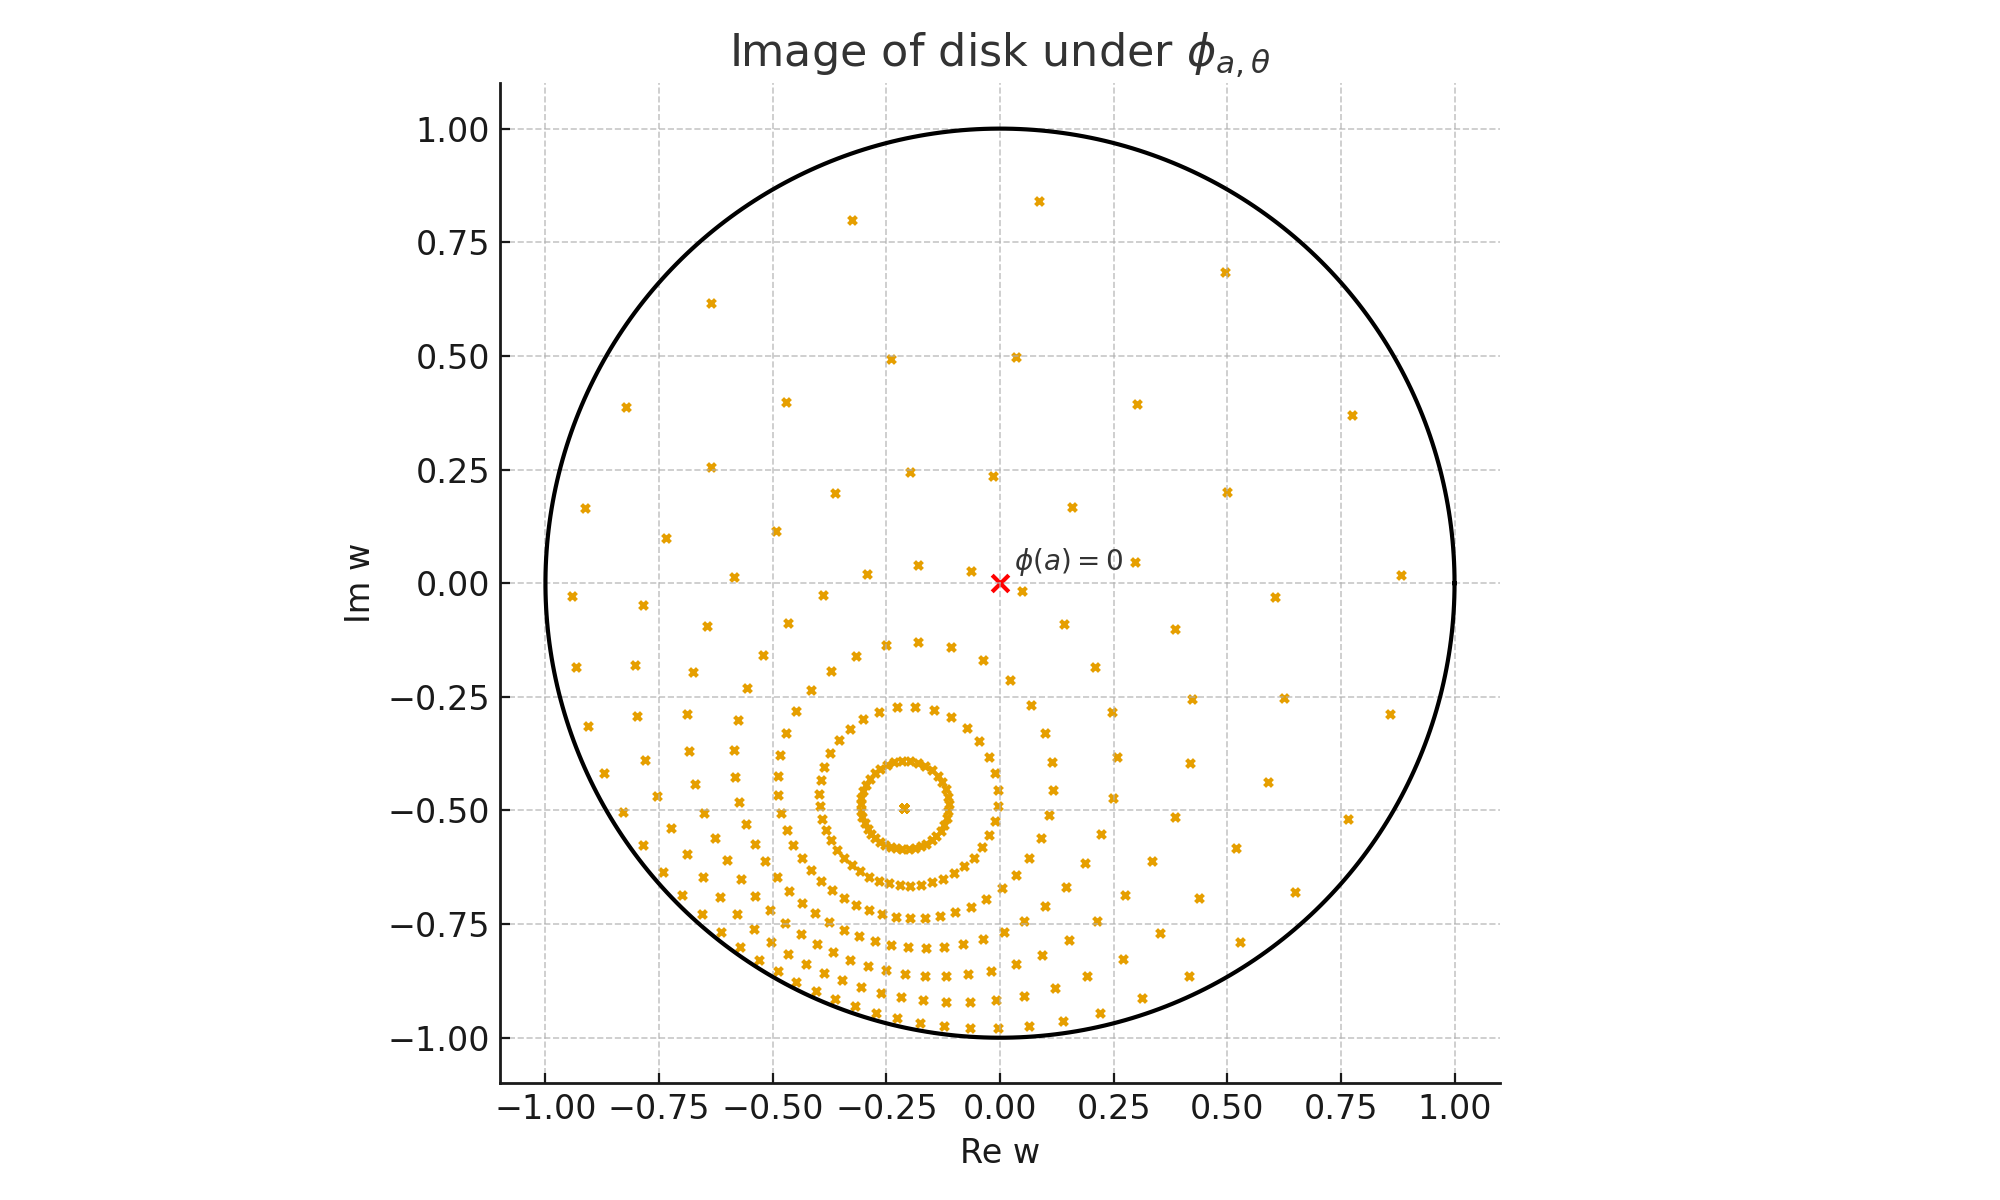
\includegraphics[width=0.78\textwidth]{figures/part04/cp_iv_0115_disk_auto_w_plane.png}
  \caption{Source-backed Part IV figure: disk auto w.}
  \label{fig:disk-auto-w}
\end{figure}

\begin{figure}[ht]
  \centering
  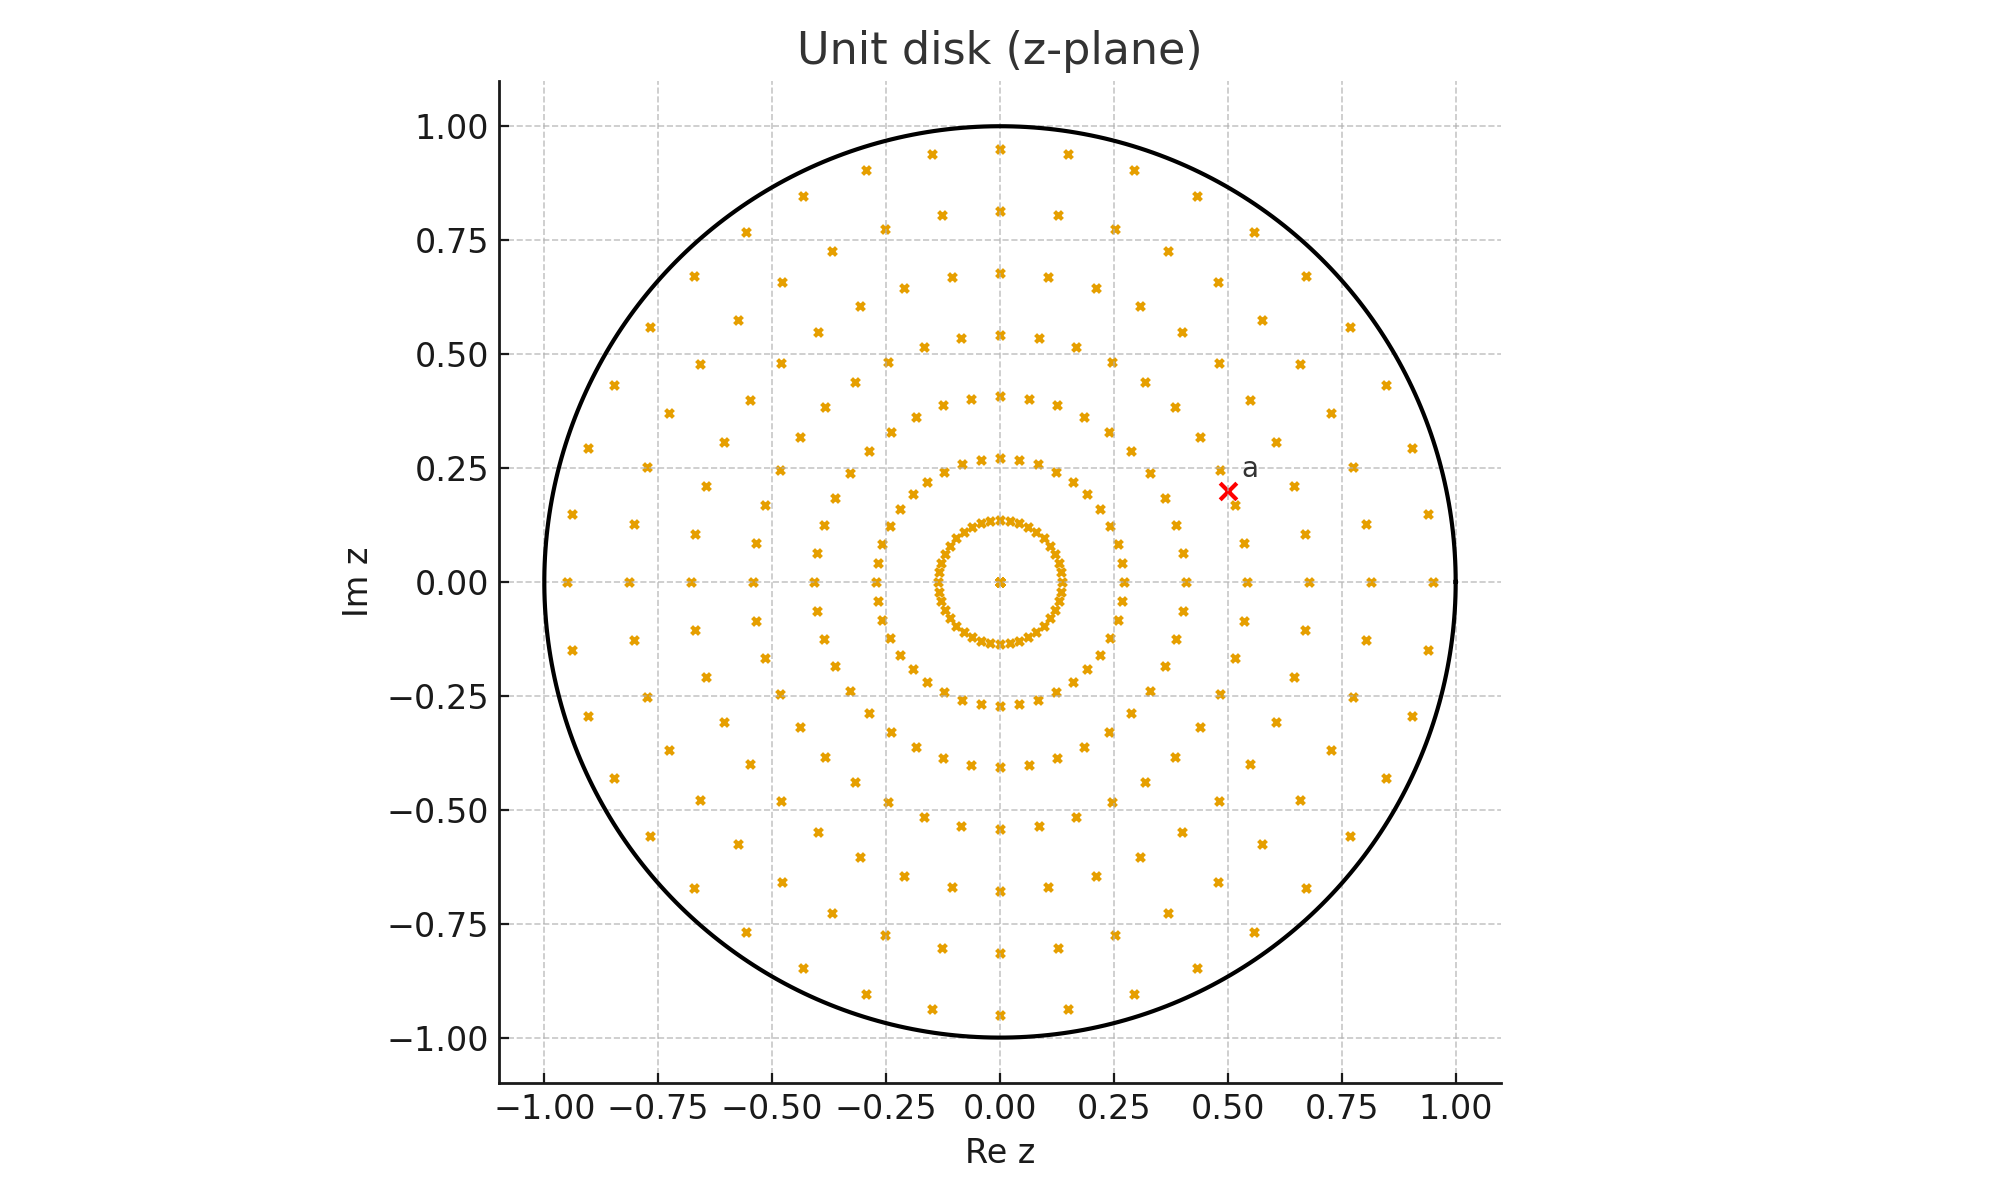
\includegraphics[width=0.78\textwidth]{figures/part04/cp_iv_0115_disk_auto_z_plane.png}
  \caption{Source-backed Part IV figure: disk auto z.}
  \label{fig:disk-auto-z}
\end{figure}

\begin{solution}
Write
\[
a=0.5+0.2i,
\qquad
\theta=\frac{\pi}{4},
\]
and
\[
\phi(z)
=
e^{i\theta}\frac{z-a}{1-\overline a\,z}.
\]
Clearly
\[
\phi(a)=0.
\]

The standard disk-automorphism identity is
\[
1-\left|
\frac{z-a}{1-\overline a\,z}
\right|^2
=
\frac{(1-|a|^2)(1-|z|^2)}
{|1-\overline a\,z|^2}.
\]
Since
\[
|a|^2=0.5^2+0.2^2=0.29<1,
\]
the right-hand side is positive exactly when \(|z|<1\). Therefore
\[
|z|<1
\quad\Longrightarrow\quad
|\phi(z)|<1,
\]
while \(|z|=1\) gives \(|\phi(z)|=1\).

The factor \(e^{i\theta}\) is a rotation and does not change moduli. The inverse map is again of disk-automorphism form, so \(\phi\) maps \(\mathbb D\) biholomorphically onto itself.

Its derivative is
\[
\phi'(z)
=
e^{i\theta}
\frac{1-|a|^2}
{(1-\overline a\,z)^2},
\]
which never vanishes on \(\mathbb D\). Hence the map is conformal. Because \(a\neq0\), it does not preserve the concentric radial/circular grid, explaining the nontrivial distortion displayed in the referenced source-backed figures.
\end{solution}



\begin{problem}[CP-IV-0119]
\label{prob:cp-iv-0119}
(Conjugation).

Let $T(z)=\bar z$. Then $A=0$, $B=1$.
The unit circle is fixed as a set, but orientation is reversed. $T$ is not complex-differentiable since $B\neq0$.
\end{problem}

\begin{solution}
For
\[
T(z)=\overline z,
\]
the decomposition
\[
T(z)=Az+B\overline z
\]
has
\[
A=0,\qquad B=1.
\]
Therefore
\[
\frac{\partial T}{\partial z}=0,
\qquad
\frac{\partial T}{\partial\overline z}=1,
\]
so \(T\) is not holomorphic.

If
\[
z=e^{it}
\]
lies on the unit circle, then
\[
T(z)=e^{-it},
\]
so the unit circle is fixed as a set, but the direction of traversal is reversed.

The real matrix is
\[
\begin{pmatrix}
1&0\\
0&-1
\end{pmatrix},
\]
whose determinant is \(-1\). Thus \(T\) reverses orientation. In fact, conjugation is the reflection of the plane across the real axis.
\end{solution}


\begin{problem}[CP-IV-0120]
\label{prob:cp-iv-0120}
\par\noindent\textbullet\quad \textbf{Total boundedness still fails (infinite dimension).}

	Closed balls in $(C^k,d_{C^k})$ are complete but not totally bounded.
	For instance, translate a fixed bump function to disjoint locations;
	the resulting family lies in the unit ball and remains pairwise well separated.
\end{problem}

\begin{solution}
Closed balls in the infinite-dimensional normed space \(C^k([a,b])\) are complete, but they are not totally bounded.

Choose a nonzero function
\[
\psi\in C_c^\infty((-1,1))
\]
and normalize it so that
\[
\|\psi^{(k)}\|_\infty=1.
\]
Choose pairwise disjoint intervals
\[
I_n=(c_n-h_n,c_n+h_n)\subset(a,b)
\]
with \(0<h_n\le1\). Define
\[
f_n(x)
=
c\,h_n^k
\psi\!\left(\frac{x-c_n}{h_n}\right),
\]
where \(c>0\) is chosen small enough that
\[
\|f_n\|_{C^k}\le1
\]
for every \(n\). Indeed,
\[
f_n^{(j)}(x)
=
c\,h_n^{k-j}
\psi^{(j)}\!\left(\frac{x-c_n}{h_n}\right),
\]
so all derivatives through order \(k\) are uniformly bounded.

Because the supports are disjoint, if \(x_n\in I_n\) is chosen so that
\[
|f_n^{(k)}(x_n)|=c,
\]
then for \(m\neq n\),
\[
f_m^{(k)}(x_n)=0.
\]
Hence
\[
\|f_n-f_m\|_{C^k}
\ge
\|f_n^{(k)}-f_m^{(k)}\|_\infty
\ge c.
\]
Thus the unit ball contains an infinite \(c\)-separated family. It cannot have a finite \(c/3\)-net, and therefore is not totally bounded.

The informal phrase ``translate a fixed bump to disjoint locations'' from the problem text needs this rescaling on the compact interval: infinitely many fixed-width supports cannot be pairwise disjoint in \([a,b]\), but shrinking supports while scaling the amplitude as above gives the required example.
\end{solution}


\begin{problem}[CP-IV-0121]
\label{prob:cp-iv-0121}
Compute $\displaystyle \int_{0}^{2\pi} e^{\,e^{it}}\,dt$.

Let $z=e^{it}$ so that $|z|=1$ and $dt=\frac{dz}{iz}$. Then
\[
\int_{0}^{2\pi} e^{e^{it}}\,dt
=\frac1i\oint_{|z|=1}\frac{e^{z}}{z}\,dz.
\]
By Cauchy’s integral formula for $f(z)=e^{z}$,
\[
\oint_{|z|=1}\frac{e^{z}}{z}\,dz=2\pi i\,f(0)=2\pi i.
\]
Hence
\[
\boxed{\displaystyle \int_{0}^{2\pi} e^{\,e^{it}}\,dt=2\pi }.
\]

Since $e^{e^{it}}=\sum_{n=0}^\infty \frac{e^{int}}{n!}$, the integral over $[0,2\pi]$
kills all terms with $n\neq0$ and equals $2\pi$.
\end{problem}

\begin{solution}
Let
\[
z=e^{it},
\qquad
0\le t\le2\pi.
\]
Then
\[
dz=iz\,dt,
\qquad
dt=\frac{dz}{iz}.
\]
Therefore
\[
\int_0^{2\pi}e^{e^{it}}\,dt
=
\frac1i
\oint_{|z|=1}\frac{e^z}{z}\,dz.
\]
By Cauchy's integral formula,
\[
\oint_{|z|=1}\frac{e^z}{z}\,dz
=
2\pi i\,e^0
=
2\pi i.
\]
Hence
\[
\boxed{
\int_0^{2\pi}e^{e^{it}}\,dt=2\pi.
}
\]

Equivalently,
\[
e^{e^{it}}
=
\sum_{n=0}^{\infty}\frac{e^{int}}{n!},
\]
and uniform convergence allows termwise integration. Every Fourier mode with \(n\ge1\) integrates to \(0\), leaving only the constant term:
\[
\int_0^{2\pi}1\,dt=2\pi.
\]
\end{solution}


\begin{problem}[CP-IV-0122]
\label{prob:cp-iv-0122}
\par\noindent\textbullet\quad $U=(0,1)\cup(2,3)$.
\end{problem}

\begin{solution}
Let
\[
U=(0,1)\cup(2,3)\subset\mathbb R.
\]
Each interval is open, so \(U\), being a union of open sets, is open.

It is not closed. For example,
\[
1-\frac1n\in(0,1)\subset U
\]
for every sufficiently large \(n\), but
\[
1-\frac1n\longrightarrow1,
\qquad
1\notin U.
\]
Thus \(U\) does not contain all of its limit points.

Therefore
\[
\boxed{
U\text{ is open and not closed in }\mathbb R.
}
\]
Its closure is
\[
\overline U=[0,1]\cup[2,3].
\]
\end{solution}


\begin{problem}[CP-IV-0125]
\label{prob:cp-iv-0125}
Let $(X,d)$ be a metric space.

		\par\noindent\textbullet\quad Show that $U\subset X$ is open in $X$ if and only if $U$ is a neighborhood of all of its points; i.e., for every $x\in U$ there exists $r>0$ with $B(x,r)\subset U$.
		\par\noindent\textbullet\quad Show that $A\subset X$ is closed in $X$ if and only if
		\[
		A=\{x\in X:\ \inf_{y\in A} d(x,y)=0\}.
		\]

	For $E\subset X$ and $x\in X$, define the point-to-set distance
	\[
	d(x,E):=\inf\{d(x,y):y\in E\}\in[0,\infty].
	\]
	The open ball is $B(x,r)=\{y\in X: d(x,y)<r\}$. A set $U$ is \emph{open} if for each $x\in U$ there exists $r>0$ with $B(x,r)\subset U$. A set $F$ is \emph{closed} if $X\setminus F$ is open, equivalently if $F$ contains all of its limit points. The closure $\overline{E}$ is the set of all $x$ such that every open ball around $x$ meets $E$.

	\bigskip
\end{problem}

\begin{solution}
\emph{($\Rightarrow$)} Suppose $U$ is open and let $x\in U$. By the metric-space definition of open, there exists $r>0$ with $B(x,r)\subset U$. Thus $U$ is a neighborhood of $x$. Since $x$ was arbitrary, $U$ is a neighborhood of each of its points.

	\smallskip
	\noindent
	\emph{($\Leftarrow$)} Conversely, assume that for every $x\in U$ there exists $r_x>0$ with $B(x,r_x)\subset U$. This is precisely the definition that $U$ is open in a metric space. Hence $U$ is open.

	\bigskip
\end{solution}

\begin{problem}[CP-IV-0127]
\label{prob:cp-iv-0127}
\par\noindent\textbullet\quad \textbf{Concrete identity.}

	With $f(x)=\sin x$ on $[0,1]$,
	\[
	T(f)(x)=\int_0^x\sin y\,dy = 1-\cos x,
	\]
	so $D(T(f))=f$, while $D(f)=\cos x$ and
	\[
	T(D(f))(x)=\int_0^x \cos y\,dy=\sin x=f(x).
	\]
\end{problem}

\begin{solution}
Let
\[
T(f)(x)=\int_0^x f(y)\,dy
\]
and let
\[
D(f)=f'.
\]
For
\[
f(x)=\sin x,
\]
we obtain
\[
T(f)(x)
=
\int_0^x\sin y\,dy
=
1-\cos x.
\]
Therefore
\[
D(T(f))(x)=\sin x=f(x).
\]
Thus
\[
D\circ T=\operatorname{id}
\]
on continuous functions for which \(T\) is defined.

On the other hand,
\[
D(f)=\cos x,
\]
so
\[
T(D(f))(x)
=
\int_0^x\cos y\,dy
=
\sin x
=
f(x),
\]
because here \(f(0)=0\).

More generally,
\[
T(Df)(x)
=
\int_0^x f'(y)\,dy
=
f(x)-f(0).
\]
Thus \(T\circ D\) is the identity precisely on functions satisfying the chosen base-point condition \(f(0)=0\).
\end{solution}


\begin{problem}[CP-IV-0128]
\label{prob:cp-iv-0128}
\par\noindent\textbullet\quad $\{(x,y): y/x\in\mathbb{Q}\}\ \cup\ \{(x,y): x=0\}$.
\end{problem}

\begin{solution}
\par\medskip\noindent\textbf{(a) $\{y>0\}$.}\quad 
Open, not closed. It is the preimage of $(0,\infty)$ under the continuous map $(x,y)\mapsto y$, and its closure is $\{y\ge0\}$.

\par\medskip\noindent\textbf{(b) $\{y\ne0\}$.}\quad 
Open, not closed. It is $\mathbb{R}^2\setminus\{y=0\}$; the $x$--axis $\{y=0\}$ is closed, hence the set is open. The axis is not open, so the set is not closed.

\par\medskip\noindent\textbf{(c) $\{(x,0): 0\le x\le1\}$.}\quad 
Closed, not open. It equals $\{y=0\}\cap\{0\le x\le1\}$ where both factors are closed (the latter is the preimage of $[0,1]$ under the $x$--projection). Any open ball in $\mathbb{R}^2$ leaves the $x$--axis, so the set is not open.

\par\medskip\noindent\textbf{(d) $\{(x,0): 0<x<1\}$.}\quad 
Neither open nor closed. It has empty interior in $\mathbb{R}^2$ (hence not open), and its closure is the closed segment in (c), so it is not closed.

\par\medskip\noindent\textbf{(e) $\{y/x\in\mathbb{N}\}\cup\{x=0\}$.}\quad 
Closed, not open. Each line $\{y=nx\}$ ($n\in\mathbb{N}$) and the axis $\{x=0\}$ is closed; to see the union is closed, let $(x_k,y_k)$ be in the union with $(x_k,y_k)\to (a,b)$. If $a=0$ the limit lies on $\{x=0\}$. If $a\ne0$, then $x_k\to a$, and the slopes $n_k=y_k/x_k\in\mathbb{N}$ cannot diverge (else $|y_k|=|n_k x_k|\to\infty$), so eventually $n_k$ is constant, say $n$, hence $b=na$. Thus the limit lies in the union. No line has interior, so the set is not open.

\par\medskip\noindent\textbf{(f) $\{y/x\in\mathbb{Q}\}\cup\{x=0\}$.}\quad 
Neither open nor closed. Not open because it is a union of lines with empty interior. Not closed because rationals are dense: pick $q_k\in\mathbb{Q}$ with $q_k\to \alpha\notin\mathbb{Q}$ and choose $x_k\to a\ne0$; then $(x_k,q_k x_k)$ belong to the set and $(x_k,q_k x_k)\to (a,\alpha a)\notin$ the set.
\end{solution}

\begin{problem}[CP-IV-0130]
\label{prob:cp-iv-0130}
\par\noindent\textbullet\quad \textbf{Derivative map is $1$-Lipschitz $C^{k+1}\!\to C^{k}$.}

	For $f,g\in C^{k+1}$ we have
	\[
	d_{C^{k}}(f',g')
	=\sum_{j=0}^{k} \|f^{(j+1)}-g^{(j+1)}\|_\infty
	\;\le\;
	\sum_{j=0}^{k+1} \|f^{(j)}-g^{(j)}\|_\infty
	= d_{C^{k+1}}(f,g).
	\]

	\medskip
\end{problem}

\begin{solution}
For \(f,g\in C^{k+1}([a,b])\),
\[
d_{C^k}(f',g')
=
\sum_{j=0}^{k}
\left\|
(f'-g')^{(j)}
\right\|_\infty.
\]
Since
\[
(f'-g')^{(j)}
=
f^{(j+1)}-g^{(j+1)},
\]
we have
\[
d_{C^k}(f',g')
=
\sum_{j=0}^{k}
\|f^{(j+1)}-g^{(j+1)}\|_\infty.
\]
This is obtained from
\[
d_{C^{k+1}}(f,g)
=
\sum_{j=0}^{k+1}
\|f^{(j)}-g^{(j)}\|_\infty
\]
by omitting the nonnegative \(j=0\) term. Hence
\[
\boxed{
d_{C^k}(f',g')
\le
d_{C^{k+1}}(f,g).
}
\]
Therefore
\[
D:C^{k+1}([a,b])\to C^k([a,b])
\]
is \(1\)-Lipschitz, and in particular continuous.
\end{solution}


\begin{problem}[CP-IV-0131]
\label{prob:cp-iv-0131}
Evaluate the principal value
\[
\operatorname{PV}\int_{-\infty}^{\infty}\frac{(x+1)\cos x}{x^{2}+1}\,dx.
\]
\end{problem}

\begin{solution}
Split the integrand:
\[
\frac{(x+1)\cos x}{x^{2}+1}
=\frac{x\cos x}{x^{2}+1}+\frac{\cos x}{x^{2}+1}.
\]
The first term is odd, so its principal value integral over $\mathbb R$ is $0$.
Therefore
\[
\operatorname{PV}\!\int_{-\infty}^{\infty}\frac{(x+1)\cos x}{x^{2}+1}\,dx
=\int_{-\infty}^{\infty}\frac{\cos x}{x^{2}+1}\,dx
=\pi e^{-1}
=\frac{\pi}{e}.
\]

\par\medskip\noindent\textbf{(Residue check, optional).}\quad 
Consider $f(z)=\dfrac{e^{iz}}{z^{2}+1}$ and integrate over the upper semicircle.
The only enclosed pole is at $z=i$, with residue $\mathrm{Res}(f;i)=\dfrac{e^{i\cdot i}}{2i}
=\dfrac{e^{-1}}{2i}$. Jordan’s lemma gives
\[
\int_{-\infty}^{\infty}\frac{e^{ix}}{x^{2}+1}\,dx=2\pi i\cdot\frac{e^{-1}}{2i}=\pi e^{-1}.
\]
Taking real parts yields $\displaystyle \int_{-\infty}^{\infty}\frac{\cos x}{x^{2}+1}\,dx=\pi e^{-1}$.
\end{solution}

\begin{problem}[CP-IV-0132]
\label{prob:cp-iv-0132}
$f_n(x)=\arctan(nx)$ (each UC) $\to$ a step function, which is not UC.
\end{problem}

\begin{solution}
For each fixed \(n\), let
\[
f_n(x)=\arctan(nx).
\]
Then
\[
f_n'(x)=\frac{n}{1+n^2x^2},
\]
so
\[
|f_n'(x)|\le n.
\]
Thus \(f_n\) is Lipschitz, hence uniformly continuous, on \(\mathbb R\).

For fixed \(x\),
\[
\lim_{n\to\infty}\arctan(nx)
=
\begin{cases}
\frac{\pi}{2},&x>0,\\[1mm]
0,&x=0,\\[1mm]
-\frac{\pi}{2},&x<0.
\end{cases}
\]
Therefore the pointwise limit is the step function
\[
f(x)=
\begin{cases}
\frac{\pi}{2},&x>0,\\
0,&x=0,\\
-\frac{\pi}{2},&x<0.
\end{cases}
\]
This function is discontinuous at \(0\), hence cannot be uniformly continuous.

Thus
\[
\boxed{
\text{a pointwise limit of uniformly continuous functions need not be uniformly continuous}.
}
\]
\end{solution}


\begin{problem}[CP-IV-0136]
\label{prob:cp-iv-0136}
— gradient field (curl $=0$), circulation $=0$

Let $\phi(x,y)=x^2+y^3$ and $\mathbf F=\nabla\phi=(2x,\,3y^2)$.
Then
\[
M_x - L_y
=
\partial_x(3y^2)-\partial_y(2x)
=
0-0
=
0,
\]
so
\[
\oint_{C} (2x\,dx+3y^2\,dy)
=
\iint_{D} 0\,dA
=
0.
\]
\emph{Interpretation:} exact/gradient fields do no net work around closed curves.
\end{problem}

\begin{solution}
Let
\[
\phi(x,y)=x^2+y^3.
\]
Then
\[
\nabla\phi=(2x,3y^2),
\]
so the \(1\)-form in the problem is exact:
\[
2x\,dx+3y^2\,dy=d\phi.
\]
Therefore its integral around any closed \(C^1\) curve \(C\) is
\[
\oint_C d\phi=0.
\]

Equivalently, writing
\[
L=2x,\qquad M=3y^2,
\]
we have
\[
M_x-L_y
=
0-0
=
0.
\]
Green's theorem gives
\[
\oint_C(2x\,dx+3y^2\,dy)
=
\iint_D0\,dA
=
\boxed{0}.
\]
This is the usual path-independence of a gradient field.
\end{solution}


\section{Elliptic Functions}

\par\medskip\noindent\textbf{Related material.}\quad Volume IV, Chapters \texttt{IV/27--IV/31}.

\begin{problem}[CP-IV-0020]
\label{prob:cp-iv-0020}
Prove uniform convergence for:
\[
\text{(a)}\quad \sum_{n=1}^\infty \sqrt{n}\,e^{-nz}\ \ \text{on}\ \ \{z: 0<r\le \Re z\},
\qquad
\text{(b)}\quad \sum_{n=1}^\infty \frac{2^n}{z^n+z^{-n}}\ \ \text{on}\ \ \{z: |z|\le r<\tfrac12\}.
\]

If $|f_n(z)|\le M_n$ on a set $E$ and $\sum M_n$ converges, then $\sum f_n$ converges uniformly on $E$.
\end{problem}

\begin{solution}
\emph{(a)} For $\Re z\ge r>0$,
\[
\bigl|\sqrt{n}\,e^{-nz}\bigr|=\sqrt{n}\,e^{-n\Re z}\le \sqrt{n}\,e^{-nr}.
\]
Since $\sum_{n\ge1}\sqrt{n}\,e^{-nr}$ converges (e.g.\ ratio or root test), the M-test yields uniform convergence on $\{z:\Re z\ge r\}$.

\medskip
\emph{(b)} Rewrite
\[
\frac{2^n}{z^n+z^{-n}}=\frac{2^n z^n}{1+z^{2n}},
\]
which is entire (in particular, defined at $z=0$). For $|z|\le r<\tfrac12$,
\[
\left|\frac{2^n z^n}{1+z^{2n}}\right|
\le \frac{2^n r^n}{\,1-|z|^{2n}\,}
\le \frac{(2r)^n}{1-r^2}.
\]
Because $2r<1$, the series $\sum (2r)^n$ converges; hence, by the M-test, $\sum \dfrac{2^n}{z^n+z^{-n}}$ converges uniformly on $\{|z|\le r\}$.

\clearpage
\end{solution}

\begin{problem}[CP-IV-0060]
\label{prob:cp-iv-0060}
(Weierstrass data for catenoid and helicoid)

We use the Weierstrass representation in the $(f,g)$-form:
	\[
	X(z)=\Re\int^z \Big(\tfrac12 f(1-g^2),\ \tfrac{i}{2}f(1+g^2),\ fg\Big)\,dz,
	\]
	where $g$ is meromorphic, $f$ is holomorphic, and the resulting parametrization is conformal and minimal.

	\medskip
	\textbf{Choice of complex parameter.}
	For the given real parameters $(u,v)$, the catenoid/helicoid are conformal in $(u,v)$, and it is convenient to set
	\[
	z=v+iu.
	\]
	Thus a suitable domain is the strip
	\[
	D=\{z=v+iu\in\mathbb{C}:\ v\in\mathbb{R},\ 0<u<2\pi\}.
	\]

	\medskip
	\textbf{Catenoid.}
	Take
	\[
	g(z)=e^{z},\qquad f(z)=a e^{-z}.
	\]
	Then
	\[
	\tfrac12 f(1-g^2)=\frac{a}{2}(e^{-z}-e^{z})=-a\sinh z,\qquad
	\tfrac{i}{2}f(1+g^2)=\frac{ia}{2}(e^{-z}+e^{z})=i a\cosh z,
	\]
	and $fg=a$. Hence
	\[
	X(z)=\Re\bigl(-a\cosh z,\ i a\sinh z,\ a z\bigr).
	\]
	With $z=v+iu$ this becomes (up to a rigid motion in the $xy$-plane)
	\[
	X(u,v)=\bigl(a\cosh v\cos u,\ a\cosh v\sin u,\ a v\bigr),
	\]
	which is exactly the given catenoid parametrization (possibly after rotating by $\pi$ about the $z$-axis).

	\medskip
	\textbf{Helicoid.}
	Keep the same $g(z)=e^{z}$ but replace $f$ by $if$:
	\[
	g(z)=e^{z},\qquad f(z)= i a e^{-z}.
	\]
	This is the classical associate surface construction. Substituting yields a parametrization which, after a rigid motion
	and a harmless shift of $u$, is the given helicoid
	\[
	\phi(u,v)=\bigl(a\sinh v\cos u,\ a\sinh v\sin u,\ a u\bigr).
	\]
	(Geometrically: multiplying $f$ by $i$ rotates the Weierstrass integrand by $90^\circ$ in the associate family.)

	\bigskip
\end{problem}

% Designed Companion Part IV figure
% Intended for \input{...} beside the matching canonical problem.
\begin{figure}[ht]
\centering
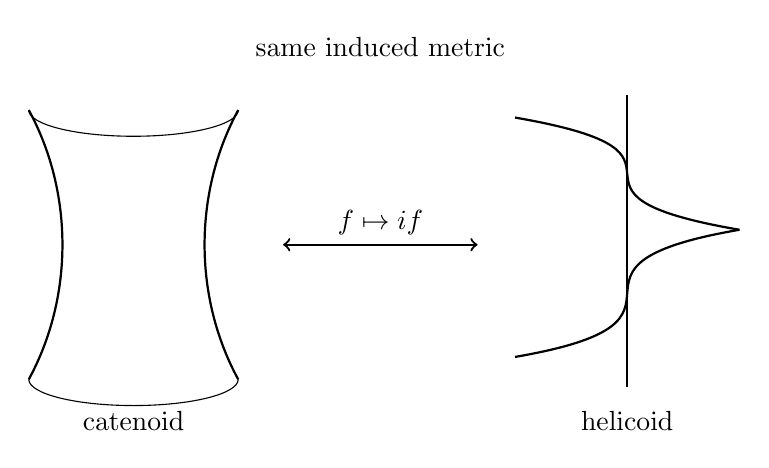
\begin{tikzpicture}[scale=0.95]
  \begin{scope}[xshift=-3.3cm]
    \draw[thick] (-1.4,-1.8) .. controls (-0.8,-0.7) and (-0.8,0.7) .. (-1.4,1.8);
    \draw[thick] (1.4,-1.8) .. controls (0.8,-0.7) and (0.8,0.7) .. (1.4,1.8);
    \draw (-1.4,-1.8) arc[start angle=180,end angle=360,x radius=1.4,y radius=0.35];
    \draw (-1.4,1.8) arc[start angle=180,end angle=360,x radius=1.4,y radius=0.35];
    \node at (0,-2.35) {catenoid};
  \end{scope}
  \draw[<->,thick] (-1.3,0)--(1.3,0) node[midway,above] {$f\mapsto if$};
  \begin{scope}[xshift=3.3cm]
    \draw[thick] (-1.5,-1.5) .. controls (1.4,-1.0) and (-1.4,-0.3) .. (1.5,0.2);
    \draw[thick] (1.5,0.2) .. controls (-1.4,0.7) and (1.4,1.2) .. (-1.5,1.7);
    \draw[thick] (0,-1.9)--(0,2.0);
    \node at (0,-2.35) {helicoid};
  \end{scope}
  \node at (0,2.65) {same induced metric};
\end{tikzpicture}
\caption{With the same Gauss-map data $g=e^z$, multiplying the Weierstrass function $f$ by $i$ moves from the catenoid to its associate helicoid. The associate pair is locally isometric.}
\label{fig:cp-iv-0060-catenoid-helicoid-associates}
\end{figure}


\begin{solution}
Use the Weierstrass representation
\[
X(z)
=
\Re\int^z
\left(
\frac12f(1-g^2),
\frac{i}{2}f(1+g^2),
fg
\right)\,dz.
\]
Take
\[
z=v+iu,
\qquad
g(z)=e^z,
\qquad
f(z)=ae^{-z}.
\]
Then
\[
\frac12f(1-g^2)=-a\sinh z,
\qquad
\frac{i}{2}f(1+g^2)=ia\cosh z,
\qquad
fg=a.
\]
An antiderivative is
\[
\left(
-a\cosh z,\,
ia\sinh z,\,
az
\right).
\]
Taking real parts with \(z=v+iu\) gives
\[
\left(
-a\cosh v\cos u,\,
-a\cosh v\sin u,\,
av
\right),
\]
which differs from
\[
\bigl(
a\cosh v\cos u,\,
a\cosh v\sin u,\,
av
\bigr)
\]
only by a rotation through \(\pi\) about the \(z\)-axis. Thus these data produce the catenoid.

For the associated surface, replace \(f\) by
\[
f_\theta=e^{-i\theta}f.
\]
At
\[
\theta=\frac{\pi}{2},
\]
one may take
\[
f_{\pi/2}=-iae^{-z},
\qquad
g=e^z.
\]
The resulting immersion is, after a rotation in the \(xy\)-plane,
\[
\boxed{
\bigl(
a\sinh v\cos u,\,
a\sinh v\sin u,\,
au
\bigr),
}
\]
the standard helicoid.

Multiplying \(f\) by a unit complex number does not change the metric because
\[
ds^2
=
\frac{|f|^2(1+|g|^2)^2}{4}|dz|^2
\]
depends only on \(|f|\). Hence the catenoid and helicoid are locally isometric members of the same associate family.

With the opposite phase \(+i\) instead of \(-i\), one obtains the reflected helicoid; this is the same associate surface up to an ambient rigid reflection/orientation convention.
\end{solution}

